\PassOptionsToPackage{unicode=true}{hyperref} % options for packages loaded elsewhere
\PassOptionsToPackage{hyphens}{url}
%
\documentclass[]{book}
\usepackage{lmodern}
\usepackage{amssymb,amsmath}
\usepackage{ifxetex,ifluatex}
\usepackage{fixltx2e} % provides \textsubscript
\ifnum 0\ifxetex 1\fi\ifluatex 1\fi=0 % if pdftex
  \usepackage[T1]{fontenc}
  \usepackage[utf8]{inputenc}
  \usepackage{textcomp} % provides euro and other symbols
\else % if luatex or xelatex
  \usepackage{unicode-math}
  \defaultfontfeatures{Ligatures=TeX,Scale=MatchLowercase}
\fi
% use upquote if available, for straight quotes in verbatim environments
\IfFileExists{upquote.sty}{\usepackage{upquote}}{}
% use microtype if available
\IfFileExists{microtype.sty}{%
\usepackage[]{microtype}
\UseMicrotypeSet[protrusion]{basicmath} % disable protrusion for tt fonts
}{}
\IfFileExists{parskip.sty}{%
\usepackage{parskip}
}{% else
\setlength{\parindent}{0pt}
\setlength{\parskip}{6pt plus 2pt minus 1pt}
}
\usepackage{hyperref}
\hypersetup{
            pdftitle={Multivariate Statistics},
            pdfauthor={Prof.~Richard Wilkinson},
            pdfborder={0 0 0},
            breaklinks=true}
\urlstyle{same}  % don't use monospace font for urls
\usepackage{color}
\usepackage{fancyvrb}
\newcommand{\VerbBar}{|}
\newcommand{\VERB}{\Verb[commandchars=\\\{\}]}
\DefineVerbatimEnvironment{Highlighting}{Verbatim}{commandchars=\\\{\}}
% Add ',fontsize=\small' for more characters per line
\usepackage{framed}
\definecolor{shadecolor}{RGB}{248,248,248}
\newenvironment{Shaded}{\begin{snugshade}}{\end{snugshade}}
\newcommand{\AlertTok}[1]{\textcolor[rgb]{0.94,0.16,0.16}{#1}}
\newcommand{\AnnotationTok}[1]{\textcolor[rgb]{0.56,0.35,0.01}{\textbf{\textit{#1}}}}
\newcommand{\AttributeTok}[1]{\textcolor[rgb]{0.77,0.63,0.00}{#1}}
\newcommand{\BaseNTok}[1]{\textcolor[rgb]{0.00,0.00,0.81}{#1}}
\newcommand{\BuiltInTok}[1]{#1}
\newcommand{\CharTok}[1]{\textcolor[rgb]{0.31,0.60,0.02}{#1}}
\newcommand{\CommentTok}[1]{\textcolor[rgb]{0.56,0.35,0.01}{\textit{#1}}}
\newcommand{\CommentVarTok}[1]{\textcolor[rgb]{0.56,0.35,0.01}{\textbf{\textit{#1}}}}
\newcommand{\ConstantTok}[1]{\textcolor[rgb]{0.00,0.00,0.00}{#1}}
\newcommand{\ControlFlowTok}[1]{\textcolor[rgb]{0.13,0.29,0.53}{\textbf{#1}}}
\newcommand{\DataTypeTok}[1]{\textcolor[rgb]{0.13,0.29,0.53}{#1}}
\newcommand{\DecValTok}[1]{\textcolor[rgb]{0.00,0.00,0.81}{#1}}
\newcommand{\DocumentationTok}[1]{\textcolor[rgb]{0.56,0.35,0.01}{\textbf{\textit{#1}}}}
\newcommand{\ErrorTok}[1]{\textcolor[rgb]{0.64,0.00,0.00}{\textbf{#1}}}
\newcommand{\ExtensionTok}[1]{#1}
\newcommand{\FloatTok}[1]{\textcolor[rgb]{0.00,0.00,0.81}{#1}}
\newcommand{\FunctionTok}[1]{\textcolor[rgb]{0.00,0.00,0.00}{#1}}
\newcommand{\ImportTok}[1]{#1}
\newcommand{\InformationTok}[1]{\textcolor[rgb]{0.56,0.35,0.01}{\textbf{\textit{#1}}}}
\newcommand{\KeywordTok}[1]{\textcolor[rgb]{0.13,0.29,0.53}{\textbf{#1}}}
\newcommand{\NormalTok}[1]{#1}
\newcommand{\OperatorTok}[1]{\textcolor[rgb]{0.81,0.36,0.00}{\textbf{#1}}}
\newcommand{\OtherTok}[1]{\textcolor[rgb]{0.56,0.35,0.01}{#1}}
\newcommand{\PreprocessorTok}[1]{\textcolor[rgb]{0.56,0.35,0.01}{\textit{#1}}}
\newcommand{\RegionMarkerTok}[1]{#1}
\newcommand{\SpecialCharTok}[1]{\textcolor[rgb]{0.00,0.00,0.00}{#1}}
\newcommand{\SpecialStringTok}[1]{\textcolor[rgb]{0.31,0.60,0.02}{#1}}
\newcommand{\StringTok}[1]{\textcolor[rgb]{0.31,0.60,0.02}{#1}}
\newcommand{\VariableTok}[1]{\textcolor[rgb]{0.00,0.00,0.00}{#1}}
\newcommand{\VerbatimStringTok}[1]{\textcolor[rgb]{0.31,0.60,0.02}{#1}}
\newcommand{\WarningTok}[1]{\textcolor[rgb]{0.56,0.35,0.01}{\textbf{\textit{#1}}}}
\usepackage{longtable,booktabs}
% Fix footnotes in tables (requires footnote package)
\IfFileExists{footnote.sty}{\usepackage{footnote}\makesavenoteenv{longtable}}{}
\usepackage{graphicx,grffile}
\makeatletter
\def\maxwidth{\ifdim\Gin@nat@width>\linewidth\linewidth\else\Gin@nat@width\fi}
\def\maxheight{\ifdim\Gin@nat@height>\textheight\textheight\else\Gin@nat@height\fi}
\makeatother
% Scale images if necessary, so that they will not overflow the page
% margins by default, and it is still possible to overwrite the defaults
% using explicit options in \includegraphics[width, height, ...]{}
\setkeys{Gin}{width=\maxwidth,height=\maxheight,keepaspectratio}
\setlength{\emergencystretch}{3em}  % prevent overfull lines
\providecommand{\tightlist}{%
  \setlength{\itemsep}{0pt}\setlength{\parskip}{0pt}}
\setcounter{secnumdepth}{5}
% Redefines (sub)paragraphs to behave more like sections
\ifx\paragraph\undefined\else
\let\oldparagraph\paragraph
\renewcommand{\paragraph}[1]{\oldparagraph{#1}\mbox{}}
\fi
\ifx\subparagraph\undefined\else
\let\oldsubparagraph\subparagraph
\renewcommand{\subparagraph}[1]{\oldsubparagraph{#1}\mbox{}}
\fi

% set default figure placement to htbp
\makeatletter
\def\fps@figure{htbp}
\makeatother

\usepackage{booktabs}
\usepackage{amsthm}
\DeclareMathOperator*{\argmin}{argmin}
\newcommand{\test}{\mathrm{test}}
\usepackage{titling}
\pretitle{\begin{center} \includegraphics[width=2in,height=2in]{figs/UoN_Primary_Logo_RGB.png}\LARGE\\}
\posttitle{\end{center}}
\usepackage{booktabs}
\usepackage{longtable}
\usepackage{array}
\usepackage{multirow}
\usepackage{wrapfig}
\usepackage{float}
\usepackage{colortbl}
\usepackage{pdflscape}
\usepackage{tabu}
\usepackage{threeparttable}
\usepackage{threeparttablex}
\usepackage[normalem]{ulem}
\usepackage{makecell}
\usepackage[]{natbib}
\bibliographystyle{apalike}

\title{Multivariate Statistics}
\author{Prof.~Richard Wilkinson}
\date{Spring 2021}

\usepackage{amsthm}
\newtheorem{theorem}{Theorem}[chapter]
\newtheorem{lemma}{Lemma}[chapter]
\newtheorem{corollary}{Corollary}[chapter]
\newtheorem{proposition}{Proposition}[chapter]
\newtheorem{conjecture}{Conjecture}[chapter]
\theoremstyle{definition}
\newtheorem{definition}{Definition}[chapter]
\theoremstyle{definition}
\newtheorem{example}{Example}[chapter]
\theoremstyle{definition}
\newtheorem{exercise}{Exercise}[chapter]
\theoremstyle{remark}
\newtheorem*{remark}{Remark}
\newtheorem*{solution}{Solution}
\begin{document}
\maketitle

{
\setcounter{tocdepth}{1}
\tableofcontents
}
\hypertarget{introduction}{%
\chapter*{Introduction}\label{introduction}}
\addcontentsline{toc}{chapter}{Introduction}

\newcommand{\bY}{\boldsymbol Y}
\newcommand{\bx}{\boldsymbol x}
\newcommand{\bX}{\boldsymbol X}
\newcommand{\bH}{\boldsymbol H}
\newcommand{\by}{\boldsymbol y}
\newcommand{\bz}{\boldsymbol z}
\newcommand{\bS}{\boldsymbol S}
\newcommand{\bR}{\boldsymbol R}
\newcommand{\bF}{\boldsymbol F}
\newcommand{\bI}{\boldsymbol I}
\newcommand{\bmu}{\boldsymbol \mu}
\newcommand{\bSigma}{\boldsymbol \Sigma}
\newcommand{\bLambda}{\boldsymbol \Lambda}
\newcommand{\bgamma}{\boldsymbol \gamma}
\newcommand{\btheta}{\boldsymbol \theta}
\newcommand{\bdelta}{\boldsymbol \delta}
\newcommand{\blambda}{\boldsymbol \lambda}
\newcommand{\bA}{\boldsymbol A}
\newcommand{\bB}{\boldsymbol B}
\newcommand{\bD}{\boldsymbol D}
\newcommand{\bE}{\boldsymbol E}
\newcommand{\bM}{\boldsymbol M}
\newcommand{\bP}{\boldsymbol P}
\newcommand{\bQ}{\boldsymbol Q}
\newcommand{\bT}{\boldsymbol T}
\newcommand{\bV}{\boldsymbol V}
\newcommand{\bW}{\boldsymbol W}
\newcommand{\bZ}{\boldsymbol Z}

\newcommand{\ba}{\boldsymbol a}
\newcommand{\bb}{\boldsymbol b}
\newcommand{\bc}{\boldsymbol c}
\newcommand{\bd}{\boldsymbol d}
\newcommand{\bh}{\boldsymbol h}
\newcommand{\bk}{\boldsymbol k}
\newcommand{\bp}{\boldsymbol p}
\newcommand{\bq}{\boldsymbol q}
\newcommand{\br}{\boldsymbol r}
\newcommand{\bu}{\boldsymbol u}
\newcommand{\bv}{\boldsymbol v}
\newcommand{\bzero}{\boldsymbol 0}
\newcommand{\mR}{\mathbb R}
\newcommand{\cR}{\mathcal R}

\newcommand{\bs}{\boldsymbol}
\newcommand{\ds}{\displaystyle}
\newcommand{\tdiag}{\text{diag}}
\newcommand{\ttr}{\text{tr}}
\newcommand{\tmin}{\text{min}}
\newcommand{\tmax}{\text{max}}
\newcommand{\tdet}{\text{det}}

\newcommand{\tcov}{\text{cov}}
\newcommand{\texp}{\text{exp}}
\newcommand{\lb}{\left(}
\newcommand{\rb}{\right)}
\newcommand{\lsb}{\left[}
\newcommand{\rsb}{\right]}

This module is concerned with the analysis of multivariate data, in which the response is a vector of random variables rather than a single random variable.

Part I of the module describes some basic concepts in Multivariate Analysis and gives some examples of multivariate data (in Chapter 1), and also contains a summary of the matrix algebra that will be important in this module (Chapter 2).

A theme running through the module is that of dimension reduction. In Part II we consider three types of dimension reduction: Principal Components Analysis (in Chapter 3),
whose purpose is to identify the main modes of variation in a multivariate dataset; Canonical Correlation Analysis (Chapter 4), whose purpose is to describe the association between two sets of variables; and Multidimensional Scaling (Chapter 5), in which the starting point is a set of pairwise distances, suitably defined, between the objects under study.

In Part III, we focus on methods of inference for multivariate data whose distribution is multivariate normal. First, in Chapter 6, we develop relevant distribution theory for the multivariate normal distribution. This includes a study of the Wishart distribution, which is a matrix generalisation of the chi-squared distribution, and Hotelling's \(T^2\), which can be thought of as a multivariate generalisation of the Student \(t\) distribution. Then in Chapter 7 we focus on inference in multivariate one-sample and two-sample problems in which the underlying distribution is multivariate normal, making use of the distribution theory developed in Chapter 6. In Chapter 8, we focus on the multivariate linear model in which the dependent variable (or \(y\) variable) is a vector and the error distribution is multivariate normal.

Finally, in Part IV, we focus on different methods of classification, i.e.~allocating the observations in a sample to different subsets (or groups). In Chapter 9, we focus on an approach called discriminant analysis, in which we have a training sample available, and we use this training sample to set up a suitable classification rule. In Chapter 10, we consider an alternative approach, known as cluster analysis, in which we allocate the observations into clusters (or similar subsets) when a training sample is not available.

\hypertarget{part-i-prerequisites}{%
\chapter*{PART I: Prerequisites}\label{part-i-prerequisites}}
\addcontentsline{toc}{chapter}{PART I: Prerequisites}

In Chapter \ref{stat-prelim} we explain what we mean by multivariate analysis and give some examples of multivariate data. We also introduce basic definitions and concepts such as the sample covariance matrix, the sample correlation matrix and graphical techniques. We also briefly discuss random vectors and random matrices and derive some of their elementary properties.

In Chapter \ref{linalg-prelim} we summarise the definitions, ideas and results from matrix algebra that will be needed later in the module.

\renewcommand{\bY}{\boldsymbol Y}
\renewcommand{\bx}{\boldsymbol x}
\renewcommand{\bX}{\boldsymbol X}
\renewcommand{\bH}{\boldsymbol H}
\renewcommand{\by}{\boldsymbol y}
\renewcommand{\bz}{\boldsymbol z}
\renewcommand{\bS}{\boldsymbol S}
\renewcommand{\bR}{\boldsymbol R}
\renewcommand{\bI}{\boldsymbol I}
\renewcommand{\bmu}{\boldsymbol \mu}
\renewcommand{\bSigma}{\boldsymbol \Sigma}
\renewcommand{\bLambda}{\boldsymbol \Lambda}
\renewcommand{\bgamma}{\boldsymbol \gamma}
\renewcommand{\blambda}{\boldsymbol \lambda}
\renewcommand{\bA}{\boldsymbol A}
\renewcommand{\bB}{\boldsymbol B}
\renewcommand{\bD}{\boldsymbol D}
\renewcommand{\bM}{\boldsymbol M}
\renewcommand{\bP}{\boldsymbol P}
\renewcommand{\bQ}{\boldsymbol Q}
\renewcommand{\bT}{\boldsymbol T}
\renewcommand{\bW}{\boldsymbol W}
\renewcommand{\ba}{\boldsymbol a}
\renewcommand{\bb}{\boldsymbol b}
\renewcommand{\bc}{\boldsymbol c}
\renewcommand{\bd}{\boldsymbol d}
\renewcommand{\bh}{\boldsymbol h}
\renewcommand{\bp}{\boldsymbol p}
\renewcommand{\bq}{\boldsymbol q}
\renewcommand{\bu}{\boldsymbol u}
\renewcommand{\bzero}{\boldsymbol 0}
\renewcommand{\mR}{\mathbb R}
\renewcommand{\cR}{\mathcal R}

\renewcommand{\bs}{\boldsymbol}
\renewcommand{\ds}{\displaystyle}
\renewcommand{\tdiag}{\text{diag}}
\renewcommand{\ttr}{\text{tr}}
\renewcommand{\tmin}{\text{min}}
\renewcommand{\tmax}{\text{max}}
\renewcommand{\tdet}{\text{det}}

\renewcommand{\tcov}{\text{cov}}
\renewcommand{\texp}{\text{exp}}
\renewcommand{\lb}{\left(}
\renewcommand{\rb}{\right)}
\renewcommand{\lsb}{\left[}
\renewcommand{\rsb}{\right]}

\hypertarget{stat-prelim}{%
\chapter{Statistical Preliminaries}\label{stat-prelim}}

In this chapter blah blah

\hypertarget{multivariate-data}{%
\section{Multivariate data}\label{multivariate-data}}

What is multivariate analysis (MVA)? Analysis of data where two or more response variables are measured on each object under study. If we measure \(p\) variables on \(n\) objects then the data can be presented in a \(n \times p\) \textbf{data matrix}.

We shall often write the data matrix as \(\mathbf X\) (\(n \times p\)) where
\[
{\mathbf X}=\left[ \begin{array}{c}
\boldsymbol x_1^\top\\
\boldsymbol x_2^\top\\
..\\
..\\
..\\
\boldsymbol x_n^\top
\end{array}\right ]= [ \boldsymbol x_1, \ldots , \boldsymbol x_n]^\top.
\]

In words: the rows of \(\mathbf X\) are \(\boldsymbol x_1^\top, \ldots , \boldsymbol x_n^\top\) and the columns of \(\boldsymbol X^\top\) are
\(\boldsymbol x_1, \ldots , \boldsymbol x_n\).

In this setup, we think of the \(\boldsymbol x_1, \ldots , \boldsymbol x_n\) are being the observation vectors, and the \(p\) columns of \(\mathbf X\)
correspond to the \(p\) variables being measured.

\textbf{Important remark on notation:} Throughout the module we shall use non-bold letters, whether upper or lower case, to indicate scalar (i.e.~real-valued) quantities; lower-case letters in bold to signify column vectors; and upper case letters in bold to signify matrices. This convention for bold letters will also apply to random quantities. So, in particular, for a random vector we always use (bold) lower case, and for a random matrix we always use bold upper-case, regardless of whether we are referring to (i) the unobserved random quantity or (ii) its observed value. It should always be clear from the context which of these two interpretations (i) or (ii) is appropriate.

\begin{example}
\protect\hypertarget{exm:unnamed-chunk-1}{}{\label{exm:unnamed-chunk-1} }Football league table where \(W =\) number of wins, \(D =\) number of draws, \(F =\) number of goals scored and \(A =\) number of goals conceded for four teams.
In this example we have \(p=4\) variables \((W, D, F, A)^\top\) measured on \(n=4\) objects (teams).
\end{example}

\begin{table}[H]
\centering
\begin{tabular}{lrrrr}
\toprule
Team & W & D & F & A\\
\midrule
USA & 1 & 2 & 4 & 3\\
England & 1 & 2 & 2 & 1\\
Slovenia & 1 & 1 & 3 & 3\\
Algeria & 0 & 1 & 0 & 2\\
\bottomrule
\end{tabular}
\end{table}

\begin{example}
\protect\hypertarget{exm:unnamed-chunk-3}{}{\label{exm:unnamed-chunk-3} }Exam marks for a set of \(n\) students where \(P =\) mark in probability and \(S =\) mark in statistics.
Note that \(x_{ij}\) denotes the \(j\)th variable measured on the \(i\)th subject.
\end{example}

\begin{table}[H]
\centering
\begin{tabular}{lll}
\toprule
Student & P & S\\
\midrule
1 & $x_{11}$ & $x_{12}$\\
2 & $x_{21}$ & $x_{22}$\\
$\vdots$ & $\vdots$ & $\vdots$\\
n & $x_{n1}$ & $x_{n2}$\\
\bottomrule
\end{tabular}
\end{table}

In MVA we attempt to answer questions such as:

\begin{itemize}
\tightlist
\item
  What is the joint distribution of marks?
\item
  How can we visualise the data?
\item
  Can we simplify the data? For example, we rank football teams using \(3W+D\) and we rank students by their average module mark but is this fair? Can we reduce the dimension in a better way?
\item
  Can we use the data to discriminate, for example, between male and female students?
\end{itemize}

We could just apply standard univariate techniques to each variable in turn but this ignores possible dependencies between the variables which we must represent to draw valid conclusions.

Finally, before moving on, we ask the question: what is the difference between MVA and standard linear regression? Answer: in standard linear regression we have a scalar response variable, \(y\) say, and a vector of covariates, \(\boldsymbol x\), say. The focus of interest is on how knowledge of \(\boldsymbol x\) influences the distribution of \(y\) (in particular, the mean of \(y\)). In contrast, with MVA the focus of interest is a response vector \(\boldsymbol y\), in which all the components of \(\boldsymbol y\) are viewed as responses rather than covariates. However, there are also situations where the response is a vector \(\boldsymbol y\) but we also have covariate information \(\boldsymbol x\). This leads to study of the multivariate linear model, which we will investigate later on in Chapter ???.

\hypertarget{summary-statistics}{%
\section{Summary statistics}\label{summary-statistics}}

In univariate statistics we define the sample mean and sample variance as
\[ \bar{x} = \frac{1}{n} \sum_{i=1}^n x_i \quad \text{and} \quad s^2 = \frac{1}{n} \sum_{i=1}^n (x_i - \bar{x})^2. \]

The analogous multivariate \textbf{sample mean} and \textbf{sample covariance matrix} are direct extensions:
\[ \bar{\boldsymbol x} = \frac{1}{n} \sum_{i=1}^n \boldsymbol x_i \quad \text{and} \quad \boldsymbol S= \frac{1}{n} \sum_{i=1}^n (\boldsymbol x_i - \bar{\boldsymbol x}) (\boldsymbol x_i - \bar{\boldsymbol x})^\top, \]
where \(\boldsymbol x_i\) is the \(p\) dimensional vector denoting the \(p\) observations on the \(i\)th object.

Note that the \(j\)th entry in \(\bar{\boldsymbol x}\) is simply the (univariate) sample mean of the \(j\)th variable. Similarly, if \(s_{ab}\) is the \((a,b)\)th entry of \(\boldsymbol S\), then \(s_{jj}\) is the (univariate) sample variance of the \(j\)th variable and \(s_{ab}\) is the sample covariance of variables \(a\) and \(b\). Note that \(\boldsymbol S\) is symmetric since \(s_{ab}=s_{ba}\).

An equivalent alternative formula for \(\boldsymbol S\) is
\[\boldsymbol S= \frac{1}{n} \left(\sum_{i=1}^n \boldsymbol x_i \boldsymbol x_i^\top \right)- \bar{\boldsymbol x} \bar{\boldsymbol x}^\top.\]

Similarly, let \(\boldsymbol R\) be the \textbf{sample correlation matrix} where the \((a,b)\)th entry of \(\boldsymbol R\) is the sample correlation between variables \(a\) and \(b\), that is
\[ r_{ab} = s_{ab}/\sqrt{s_{aa}s_{bb}}. \]
Note that
\[ \boldsymbol R= \boldsymbol D^{-1} \boldsymbol S\boldsymbol D^{-1} \]
where \(\boldsymbol D= \text{diag}(\sqrt{s_{11}}, \dots, \sqrt{s_{pp}})\). Note that \(\boldsymbol R\) is symmetric, the diagonal entries are always exactly 1 (each variable is perfectly correlated with itself) and that \(|r_{ab}| \leq 1\).

Note that if we change the unit of measurement for the \(\boldsymbol x_i\)'s then \(\boldsymbol S\) will change but \(\boldsymbol R\) will not.

The \textbf{total variation} in the data set is usually measured by \(\text{tr}(\boldsymbol S)\) where \(\text{tr}()\) is the trace function that sums the diagonal elements of the matrix. That is,
\[\text{tr}(\boldsymbol S) = s_{11} + s_{22} + \ldots + s_{pp}.\]

In MVA it is much easier to work with vector and matrix notation.

\begin{example}
\protect\hypertarget{exm:unnamed-chunk-5}{}{\label{exm:unnamed-chunk-5} }The table below shows the module marks for 5 students on the modules G11PRB (\(P\)) and G11STA (\(S\)).
\end{example}

\begin{table}[H]
\centering
\begin{tabular}{lrr}
\toprule
Student & P & S\\
\midrule
A & 41 & 63\\
B & 72 & 82\\
C & 46 & 38\\
D & 77 & 57\\
E & 59 & 85\\
\bottomrule
\end{tabular}
\end{table}

Calculate the sample mean, sample covariance, sample correlation and total variation.

The sample mean is \(\bar{\boldsymbol x} = \begin{pmatrix} 59 \\ 65 \end{pmatrix}\).

The sample covariance matrix is \(\boldsymbol S= \begin{pmatrix} 197.2 & 92.8 \\ 92.8 & 297.2 \end{pmatrix}\).

The sample correlation matrix is
\begin{align*}
\boldsymbol R&= \boldsymbol D^{-1} \boldsymbol S\boldsymbol D^{-1}\\
&= \begin{pmatrix} 14.0 & 0 \\ 0 & 17.2 \end{pmatrix}^{-1} \begin{pmatrix} 197.2 & 92.8 \\ 92.8 & 297.2 \end{pmatrix} \begin{pmatrix} 14.0 & 0 \\ 0 & 17.2 \end{pmatrix}^{-1} \\
&= \begin{pmatrix} 0.071 & 0 \\ 0 & 0.058 \end{pmatrix} \begin{pmatrix} 197.2 & 92.8 \\ 92.8 & 297.2 \end{pmatrix} \begin{pmatrix} 0.071 & 0 \\ 0 & 0.058 \end{pmatrix} \\
&= \begin{pmatrix} 1.000 & 0.383 \\ 0.383 & 1.000 \end{pmatrix}.
\end{align*}

The total variation is \(\text{tr}(\boldsymbol S) = 197.2 + 297.2 = 494.4\).

To calculate these in R use, `colMeans', `cov', and `cor'. These assume each column is a different variable, and each row a different observation.

\begin{Shaded}
\begin{Highlighting}[]
\KeywordTok{library}\NormalTok{(dplyr)}
\NormalTok{Ex1 <-}\StringTok{ }\KeywordTok{data.frame}\NormalTok{(}
  \DataTypeTok{Student=}\NormalTok{LETTERS[}\DecValTok{1}\OperatorTok{:}\DecValTok{5}\NormalTok{],}
  \DataTypeTok{P =} \KeywordTok{c}\NormalTok{(}\DecValTok{41}\NormalTok{,}\DecValTok{72}\NormalTok{,}\DecValTok{46}\NormalTok{,}\DecValTok{77}\NormalTok{,}\DecValTok{59}\NormalTok{),}
  \DataTypeTok{S =} \KeywordTok{c}\NormalTok{(}\DecValTok{63}\NormalTok{,}\DecValTok{82}\NormalTok{,}\DecValTok{38}\NormalTok{,}\DecValTok{57}\NormalTok{,}\DecValTok{85}\NormalTok{)}
\NormalTok{  )}

\NormalTok{Ex1 }\OperatorTok\StringTok{ }\KeywordTok{select_if}\NormalTok{(is.numeric) }\OperatorTok\StringTok{ }\NormalTok{colMeans}
\end{Highlighting}
\end{Shaded}

\begin{verbatim}
##  P  S 
## 59 65
\end{verbatim}

\begin{Shaded}
\begin{Highlighting}[]
\NormalTok{Ex1 }\OperatorTok\StringTok{ }\KeywordTok{select_if}\NormalTok{(is.numeric) }\OperatorTok\StringTok{ }\NormalTok{cov}
\end{Highlighting}
\end{Shaded}

\begin{verbatim}
##       P     S
## P 246.5 116.0
## S 116.0 371.5
\end{verbatim}

\begin{Shaded}
\begin{Highlighting}[]
\NormalTok{Ex1 }\OperatorTok\StringTok{ }\KeywordTok{select_if}\NormalTok{(is.numeric) }\OperatorTok\StringTok{ }\NormalTok{cor}
\end{Highlighting}
\end{Shaded}

\begin{verbatim}
##           P         S
## P 1.0000000 0.3833276
## S 0.3833276 1.0000000
\end{verbatim}

NOTE R USES 1/n-1 whereas hand calculation si 1/n\ldots{}..

\hypertarget{graphical-techniques}{%
\section{Graphical techniques}\label{graphical-techniques}}

We can draw histograms and scatter plots to view the distribution when \(p=1\) and \(p=2\) respectively. For \(p \geq 3\) the task is much harder. One solution is a matrix of pair-wise scatter plots using the \texttt{pairs} command in R. The graph below shows the relationship between goals scored (F), goals against (A) and points (PT) for 20 teams during a recent Premiership season.

\begin{figure}
\centering
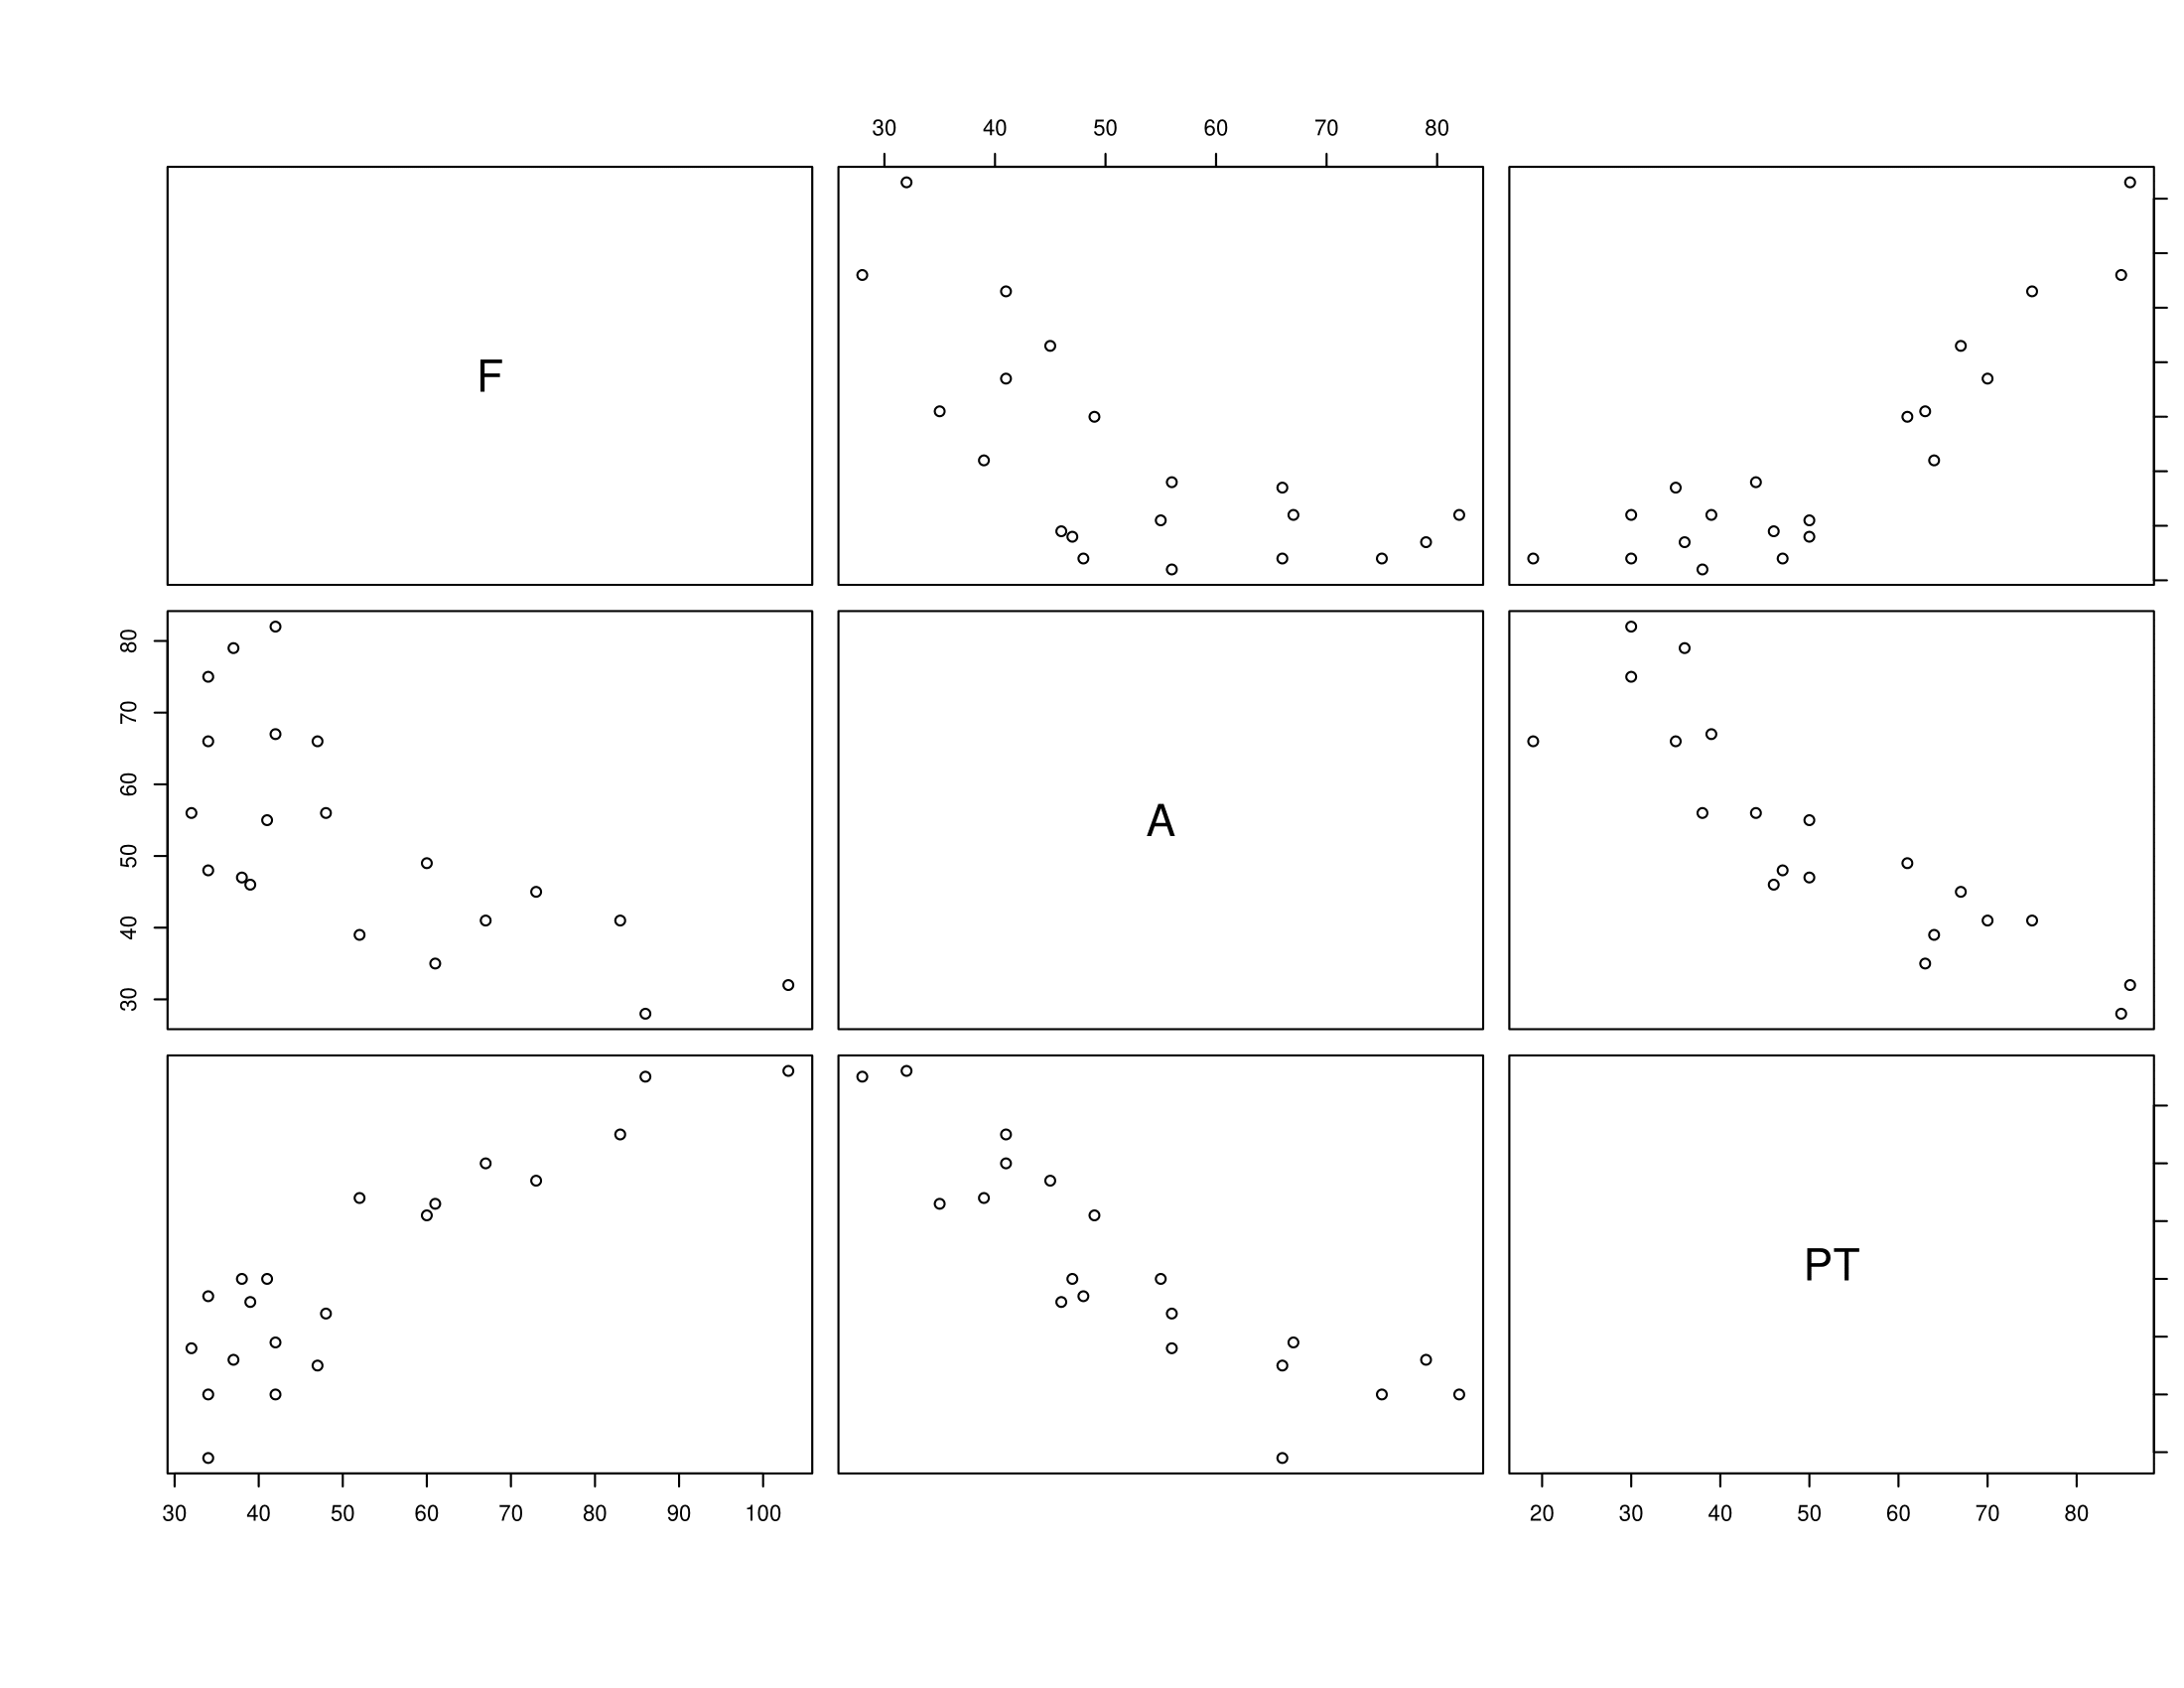
\includegraphics{figs/pairs.png}
\caption{Scatter plots}
\end{figure}

WOULD BE BETTER TO CREATE THIS FIGURE HERE

You can also use the \texttt{plot3d} command in the \texttt{rgl} library to create an interactive 3D plot of the data. The difficulty of displaying multivariate data is further motivation for developing a method for reducing the number of dimensions in the data.

\hypertarget{random-vectors-and-matrices}{%
\section{Random Vectors and Matrices}\label{random-vectors-and-matrices}}

The \emph{population mean vector} of the random vector \(\boldsymbol x\) is
\[\boldsymbol \mu= E(\boldsymbol x).\]

The \emph{population covariance matrix} of \(\boldsymbol x\) is
\[ \boldsymbol \Sigma= \text{Var}(\boldsymbol x) = E \left((\boldsymbol x-\boldsymbol \mu)(\boldsymbol x-\boldsymbol \mu)^\top \right).\]

The covariance between \(\boldsymbol x\) (\(p \times 1\)) and \(\boldsymbol y\) (\(q \times 1\)) is
\[ \text{Cov}(\boldsymbol x,\boldsymbol y) = E \left((\boldsymbol x- E(\boldsymbol x))(\boldsymbol y- E(\boldsymbol y))^\top \right). \]

Let \(\boldsymbol A\) (\(q \times p\)) denote a constant matrix and let \(\boldsymbol b\) (\(q \times 1\)) denote a constant vector. Then the following properties hold:

\begin{itemize}
\tightlist
\item
  \(E(\boldsymbol A\boldsymbol x+ \boldsymbol b) = \boldsymbol AE(\boldsymbol x) + \boldsymbol b=\boldsymbol A\boldsymbol \mu+\boldsymbol b\).
\item
  \(\boldsymbol \Sigma= E(\boldsymbol x\boldsymbol x^\top) - \boldsymbol \mu\boldsymbol \mu^\top\).
\item
  \(\text{Var}(\boldsymbol A\boldsymbol x+ \boldsymbol b) = \boldsymbol A\boldsymbol \Sigma\boldsymbol A^\top\), where \(\boldsymbol A\) is a \(q \times p\) constant matrix.
\item
  A covariance matrix \(\boldsymbol \Sigma\) is always non-negative
  definite. Moreover, \(\boldsymbol \Sigma\) is positive definite if and only
  if all its eigenvalues are positive, in which case its
  determinant is positive and \(\boldsymbol \Sigma\) is non-singular.
\item
  \(\text{Cov}(\boldsymbol x,\boldsymbol y) = E(\boldsymbol x\boldsymbol y^\top) - E(\boldsymbol x) E(\boldsymbol y)^\top\).
\item
  \(\text{Cov}(\boldsymbol x,\boldsymbol x) = \boldsymbol \Sigma\).
  \(\text{Cov}(\boldsymbol x,\boldsymbol y) = \text{Cov}(\boldsymbol y,\boldsymbol x)^\top\).
\item
  If \(\boldsymbol x\) and \(\boldsymbol y\) are independent then \(\text{Cov}(\boldsymbol x,\boldsymbol y) = {\mathbf 0}_{p,q}\).
\item
  If \(p=q\) then
  \[
  \text{Var}(\boldsymbol x+ \boldsymbol y) = \text{Var}(\boldsymbol x) + \text{Var}(\boldsymbol y) + \text{Cov}(\boldsymbol x,\boldsymbol y) + \text{Cov}(\boldsymbol y,\boldsymbol x).
  \]
\end{itemize}

\hypertarget{unbiased-estimators}{%
\section{Unbiased Estimators}\label{unbiased-estimators}}

Recall from univariate statistics that an estimator \(\hat{\theta}\) of a parameter \(\theta\) is unbiased if \(E(\hat{\theta}) = \theta\) for all \(\theta\). This concept readily transfers to the multivariate context.

\begin{proposition}
\protect\hypertarget{prp:unnamed-chunk-9}{}{\label{prp:unnamed-chunk-9} }Let \(\boldsymbol x_1, \ldots \boldsymbol x_n\) be independent and identically distributed (i.i.d.), sampled from a population with mean \(\boldsymbol \mu\) and covariance matrix \(\boldsymbol \Sigma\). If \(\bar{\boldsymbol x}\) and \(\boldsymbol S\) are the sample mean and covariance matrix, respectively, then

\begin{enumerate}
\def\labelenumi{\arabic{enumi}.}
\item
  \(E(\bar{\boldsymbol x}) = \boldsymbol \mu\).
\item
  \(\text{Var}(\bar{\boldsymbol x}) = {\displaystyle\frac{1}{n}} \boldsymbol \Sigma\).
\item
  \(E(\boldsymbol S) = {\displaystyle\frac{n-1}{n}} \boldsymbol \Sigma\).
\end{enumerate}
\end{proposition}

\begin{proof}
\iffalse{} {Proof. } \fi{}\textbf{Part 1} Since expectations behave linearly,
\[E(\bar{\boldsymbol x}) = E \left(\frac{1}{n} \sum_{i=1}^n \boldsymbol x_i \right)= \frac{1}{n} \sum_{i=1}^n E(\boldsymbol x_i) = \frac{1}{n} n \boldsymbol \mu= \boldsymbol \mu.\]
\textbf{Part 2}
We have
\begin{eqnarray*}
\text{Var}(\bar{\boldsymbol x}) &=& \text{Var} \left(\frac{1}{n} \sum_{i=1}^n \boldsymbol x_i \right)\\
&=& \sum_{i,j=1}^n \text{Cov}\left (\frac{1}{n}\boldsymbol x_i, \frac{1}{n}\boldsymbol x_j \right)\\
&=& \sum_{i=1}^n \text{Var} \left(\frac{1}{n} \boldsymbol x_i \right)+ \sum_{i \neq j} \text{Cov} \left(\frac{1}{n} \boldsymbol x_i, \frac{1}{n} \boldsymbol x_j \right)\\
&=& \frac{1}{n^2} \left(\sum_{i=1}^n \text{Var}(\boldsymbol x_i) + \sum_{i \neq j} \text{Cov}(\boldsymbol x_i,\boldsymbol x_j) \right)\\
&=& \frac{1}{n^2} \left(\sum_{i=1}^n \text{Var}(\boldsymbol x_i) \right)\\
&=& \frac{1}{n^2} n \boldsymbol \Sigma\\
&=& \frac{1}{n} \boldsymbol \Sigma.
\end{eqnarray*}

\textbf{Part 3} From the definition of the sample covariance,

\begin{eqnarray*}
\boldsymbol S&=& \frac{1}{n} \sum_{i=1}^n  (\boldsymbol x_i -\bar{\boldsymbol x})( \boldsymbol x_i - \bar{\boldsymbol x})^\top \\
&=& \frac{1}{n} \sum_{i=1}^n (\boldsymbol x_i - \boldsymbol \mu+ \boldsymbol \mu-\bar{\boldsymbol x})(\boldsymbol x_i - \boldsymbol \mu+\boldsymbol \mu-\bar{\boldsymbol x})^\top  \\
&=& \frac{1}{n} \sum_{i=1}^n \bigg \{(\boldsymbol x_i - \boldsymbol \mu)(\boldsymbol x_i - \boldsymbol \mu)^\top +(\bar{\boldsymbol x}-\boldsymbol \mu)(\bar{\boldsymbol x}-\boldsymbol \mu)^\top \\
&&  \qquad -(\boldsymbol x_i-\boldsymbol \mu)(\bar{\boldsymbol x}-\boldsymbol \mu)^\top -(\bar{\boldsymbol x}-\boldsymbol \mu)(\boldsymbol x_i-\boldsymbol \mu)^\top \bigg \}\\
&=& \frac{1}{n} \left \{\sum_{i=1}^n (\boldsymbol x_i - \boldsymbol \mu)(\boldsymbol x_i - \boldsymbol \mu)^\top \right \}- (\bar{\boldsymbol x}-\boldsymbol \mu)(\bar{\boldsymbol x}-\boldsymbol \mu)^\top
\end{eqnarray*}

Since \(E(\bar{\boldsymbol x})=\boldsymbol \mu\) and \(\text{Var}(\bar{\boldsymbol x})=n^{-1}\boldsymbol \Sigma\), it follows that

\begin{eqnarray*}
E(\boldsymbol S) &=& E\left \{\frac{1}{n}\sum_{i=1}^n  (\boldsymbol x_i - \boldsymbol \mu)(\boldsymbol x_i - \boldsymbol \mu)^\top \right \}\\
&& \qquad -E\left \{ (\bar{\boldsymbol x}-\boldsymbol \mu)(\bar{\boldsymbol x}-\boldsymbol \mu)^\top \right \}\\
&=&\left \{\frac{1}{n}\sum_{i=1}^n E \left [(\boldsymbol x_i - \boldsymbol \mu)(\boldsymbol x_i - \boldsymbol \mu)^\top \right ]\right \} -\text{Var}(\bar{\boldsymbol x})\\
&=&E \left \{(\boldsymbol x_1 - \boldsymbol \mu)(\boldsymbol x_1  - \boldsymbol \mu)^\top \right \} -\text{Var}(\bar{\boldsymbol x})\\
&=& \text{Var}(\boldsymbol x_1)-\text{Var}(\bar{\boldsymbol x}) \\
&=& \boldsymbol \Sigma- \frac{1}{n}\boldsymbol \Sigma\\
&=& \frac{n-1}{n}  \boldsymbol \Sigma,
\end{eqnarray*}

which completes the proof.\\
\end{proof}

An implication of this theorem is that \(\bar{\boldsymbol x}\) is an unbiased estimator for \(\boldsymbol \mu\) but that \(\boldsymbol S\) is a biased estimator of \(\boldsymbol \Sigma\). Note, however, that \({\displaystyle\frac{n}{n-1}} \boldsymbol S\) is an unbiased estimator of \(\boldsymbol \Sigma\), i.e.
\[
 \frac{n}{n-1}E[\boldsymbol S]=\boldsymbol \Sigma.
 \]

\hypertarget{linalg-prelim}{%
\chapter{Review of Matrix algebra}\label{linalg-prelim}}

In this chapter blah blah

\renewcommand{\bY}{\boldsymbol Y}
\renewcommand{\bx}{\boldsymbol x}
\renewcommand{\bX}{\boldsymbol X}
\renewcommand{\bH}{\boldsymbol H}
\renewcommand{\by}{\boldsymbol y}
\renewcommand{\bz}{\boldsymbol z}
\renewcommand{\bS}{\boldsymbol S}
\renewcommand{\bR}{\boldsymbol R}
\renewcommand{\bI}{\boldsymbol I}
\renewcommand{\bmu}{\boldsymbol \mu}
\renewcommand{\bSigma}{\boldsymbol \Sigma}
\renewcommand{\bLambda}{\boldsymbol \Lambda}
\renewcommand{\bgamma}{\boldsymbol \gamma}
\renewcommand{\blambda}{\boldsymbol \lambda}
\renewcommand{\bA}{\boldsymbol A}
\renewcommand{\bB}{\boldsymbol B}
\renewcommand{\bD}{\boldsymbol D}
\renewcommand{\bM}{\boldsymbol M}
\renewcommand{\bP}{\boldsymbol P}
\renewcommand{\bQ}{\boldsymbol Q}
\renewcommand{\bT}{\boldsymbol T}
\renewcommand{\bW}{\boldsymbol W}
\renewcommand{\ba}{\boldsymbol a}
\renewcommand{\bb}{\boldsymbol b}
\renewcommand{\bc}{\boldsymbol c}
\renewcommand{\bd}{\boldsymbol d}
\renewcommand{\bh}{\boldsymbol h}
\renewcommand{\bp}{\boldsymbol p}
\renewcommand{\bq}{\boldsymbol q}
\renewcommand{\bu}{\boldsymbol u}
\renewcommand{\bzero}{\boldsymbol 0}
\renewcommand{\mR}{\mathbb R}
\renewcommand{\cR}{\mathcal R}

\renewcommand{\bs}{\boldsymbol}
\renewcommand{\ds}{\displaystyle}
\renewcommand{\tdiag}{\text{diag}}
\renewcommand{\ttr}{\text{tr}}
\renewcommand{\tmin}{\text{min}}
\renewcommand{\tmax}{\text{max}}
\renewcommand{\tdet}{\text{det}}

\renewcommand{\tcov}{\text{cov}}
\renewcommand{\texp}{\text{exp}}
\renewcommand{\lb}{\left(}
\renewcommand{\rb}{\right)}
\renewcommand{\lsb}{\left[}
\renewcommand{\rsb}{\right]}

\hypertarget{basic-definitions}{%
\section{Basic definitions}\label{basic-definitions}}

The matrix \({\mathbf A}\) will be referred to in the following equivalent ways:
\begin{eqnarray*}
{\mathbf A}=\stackrel{n\times p}{\mathbf A} &=& \left[\begin{array}{cccc}
a_{11}&a_{12}&\dots&a_{1p}\\
a_{21}&a_{22}&\dots&a_{2p}\\
\vdots&\vdots&&\vdots\\
a_{n1}&a_{n2}&\dots&a_{np}
\end{array} \right] \\
&=& [a_{ij}: i=1,\dots ,n;\ j=1,\dots ,p\,]=(a_{ij}),
\end{eqnarray*}
where the \(a_{ij}\) are real numbers.

A matrix of order \(1\times 1\) is called a \emph{scalar}.

A matrix of order \(n\times 1\) is called a \emph{(column) vector}.

A matrix of order \(1\times p\) is called a \emph{(row) vector}.

e.g. \(\stackrel{n\times 1}{\mathbf a}=\left( \begin{array}{c} a_1\\\vdots\\a_n \end{array} \right)\)\quad is a column vector.

The \(n\times n\) \emph{identity matrix} \({\mathbf I}_n\) has diagonal elements equal to 1
and off-diagonal elements equal to zero.

A \emph{diagonal} matrix is an \(n \times n\) matrix whose
off-diagonal elements are zero. Sometimes we denote a diagonal
matrix by \(\text{diag}\{a_1,\ldots, a_n\}\).

\hypertarget{elementary-matrix-operations}{%
\section{Elementary matrix operations}\label{elementary-matrix-operations}}

\begin{enumerate}
\def\labelenumi{\arabic{enumi}.}
\item
  \emph{Addition/Subtraction}. If \(\stackrel{n\times p}{\mathbf A}=[a_{ij}]\) and \(\stackrel{n\times p}{\mathbf B}=[b_{ij}]\) are
  given matrices then
  \[ {\mathbf A}+{\mathbf B}=[a_{ij}+b_{ij}] \qquad \text{and} \qquad {\mathbf A}-{\mathbf B}=[a_{ij}-b_{ij}].\]
\item
  \emph{Scalar Multiplication}. If \(\lambda\) is a scalar and \({\mathbf A}=[a_{ij}]\) then
  \[\lambda {\mathbf A}=[\lambda a_{ij}].\]
\item
  \emph{Matrix Multiplication}. If \(\stackrel{n\times p}{\mathbf A}\) and \(\stackrel{p\times q}{\mathbf B}\) are
  given matrices then \({\mathbf AB}=\stackrel{n\times q}{\mathbf C}=[c_{ij}]\) where
  \[c_{ij}=\sum _{k=1}^p a_{ik}b_{kj}, \qquad i=1,\dots,n, \qquad j=1,\dots ,q.\]
\item
  \emph{Matrix Transpose}. If \(\stackrel{m \times n}{\boldsymbol A}=[a_{ij}: i=1, \ldots , m; j=1, \ldots , n]\), then the transpose of \(\boldsymbol A\), written
  \(\boldsymbol A^\top\), is given by the \(n \times m\) matrix
  \[
  \boldsymbol A^\top =[a_{ji}: j=1, \ldots , n; i=1, \ldots, m].
  \]
  Note from the definitions that \(({\mathbf AB})^\top={\mathbf B}^\top {\mathbf A}^\top\).
  In the special case in which \({\mathbf A}=\stackrel{n\times 1}{\mathbf a}\) and
  \({\mathbf B}=\stackrel{n\times 1}{\mathbf b}\), the quantity \({\mathbf A}^\top {\mathbf B}={\mathbf a}^\top {\mathbf b}\) is real-valued and is
  known as the \emph{scalar product of \(\mathbf a\) and \(\mathbf b.\)\newline 
  Note that \({\mathbf a}^\top {\mathbf a}=\sum _{i=1}^n a_i^2\geq 0\) with equality iff
  \({\mathbf a}={\mathbf 0}_n\) where \(\stackrel{n\times 1}{\mathbf 0}_n=(0,0,\dots ,0)^\top\). We may
  interpret \({\mathbf a}^\top {\mathbf a}\) as the (length)\(^2\) of the vector \({\mathbf a}\).
  The }norm* of a vector \({\mathbf a}\) is defined by
  \[||{\mathbf a}||=({\mathbf a}^\top {\mathbf a})^{1/2}.\]
  The scalar product has an alternative (but equivalent) representation:
  \[
  \boldsymbol a^\top \boldsymbol b= \vert \vert \boldsymbol a\vert \vert \cdot \vert \vert \boldsymbol b\vert \vert \cos(\theta),
  \]
  where \(\theta\) is the angle (in radians) between the vectors \(\boldsymbol a\) and \(\boldsymbol b\).\newline 
  A \emph{unit vector} \(\mathbf a\) is a vector satisfying \(||{\mathbf a}||^2= {\mathbf a}^\top {\mathbf a}=1\).\textbackslash{}
  A matrix \(\stackrel{n\times n}{\mathbf Q}\) satisfying \({\mathbf QQ}^\top = {\mathbf Q}^\top {\mathbf Q}={\mathbf I}_n\) is called an
  \emph{orthogonal matrix}. Equivalently, a matrix \(\mathbf Q\) is orthogonal iff \({\mathbf Q}^{-1}={\mathbf Q}^\top\).\newline 
  If \({\mathbf Q}=[\boldsymbol q_1,\ldots, \boldsymbol q_n]\) is an orthogonal matrix, then the columns \(\boldsymbol q_1, \ldots, \boldsymbol q_n\) are mutually orthogonal unit vectors, i.e.
  \[
  \boldsymbol q_j^\top \boldsymbol q_k=\begin{cases} 1 &\hbox{ if }  j=k\\
  0 &\hbox{ if }   j \neq k \\
  \end{cases}
  \]
\end{enumerate}

\begin{proposition}
\protect\hypertarget{prp:two1}{}{\label{prp:two1} }If \(\boldsymbol q_1, \ldots , \boldsymbol q_n\) are mutually orthogonal \(n \times 1\) unit vectors then
\[
\sum_{i=1}^n \boldsymbol q_i \boldsymbol q_i^\top = {\mathbf I}_n,
\]
the \(n \times n\) identity matrix.
\end{proposition}

\begin{enumerate}
\def\labelenumi{\arabic{enumi}.}
\setcounter{enumi}{4}
\item
  \emph{Matrix Inverse}. The inverse of a matrix \(\stackrel{n\times n}{\mathbf A}\) (if it exists) is a
  matrix \(\stackrel{n\times n}{\mathbf B}\) such that \({\mathbf AB}={\mathbf BA}={\mathbf I}_n.\) We denote
  the inverse by \({\mathbf A}^{-1}\). Note that if \({\mathbf A}_1\) and \({\mathbf A}_2\) are both invertible,
  then \(({\mathbf A}_1 {\mathbf A}_2)^{-1}={\mathbf A}_2^{-1}{\mathbf A}_1^{-1}\).
\item
  \emph{Trace}. The trace of a matrix \(\stackrel{n\times n}{\mathbf A}\) is given by
  \[ \text{tr}({\mathbf A})=\sum _{i=1}^n a_{ii}.\]
\end{enumerate}

\begin{lemma}
\protect\hypertarget{lem:unnamed-chunk-1}{}{\label{lem:unnamed-chunk-1} }For any matrices \(\boldsymbol A\) (\$ n \times m\$) and \(\boldsymbol B\) (\(m \times n\)),
\[
\text{tr}(\boldsymbol A\boldsymbol B) = \text{tr}(\boldsymbol B\boldsymbol A).
\]
\end{lemma}

\hypertarget{linear-independence-and-determinants}{%
\section{Linear independence and determinants}\label{linear-independence-and-determinants}}

\noindent Vectors \(\stackrel{n\times 1}{\mathbf x}_1 ,\dots , \stackrel{n\times 1}{\mathbf x}_p\)
are said to be \emph{linearly dependent} if there exist scalars
\(\lambda _1, \dots ,\lambda _p\) not all zero such that
\[ \lambda _1 {\mathbf x}_1+\lambda _2 {\mathbf x}_2+ \dots + \lambda _p {\mathbf x}_p={\mathbf 0}.\]
Otherwise, these vectors are said to be \emph{linearly independent}.

The \emph{rank} of a matrix is equal to the maximum number of linearly independent rows (equivalently, columns).

The \emph{determinant} of a square matrix \(\stackrel{n\times n}{\mathbf A}\) is
defined as
\[ \text{det}({\mathbf A})=\sum (-1)^{|\tau |} a_{1\tau(1)}\dots a_{n\tau (n)} \]
where the summation is taken over all permutations \(\tau\) of \(\{1,2,\dots ,n\}\),
and we define \(|\tau |=0\) or \(1\) depending on whether \(\tau\) can be written as an even or
odd number of transpositions.

E.g. If \({\mathbf A}=\left[ \begin{array}{cc} a_{11}&a_{12}\\ a_{21}&a_{22} \end{array} \right]\),
then \(\text{det}({\mathbf A})=a_{11}a_{22}-a_{12}a_{21}\).

\begin{proposition}
\protect\hypertarget{prp:unnamed-chunk-2}{}{\label{prp:unnamed-chunk-2} }For any matrices \(\stackrel{n\times n}{\mathbf A}\),
\(\stackrel{n\times n}{\mathbf B}\), \(\stackrel{n\times n}{\mathbf C}\) such that \({\mathbf C}={\mathbf{AB}}\),
\[ \text{det}({\mathbf C})=\text{det}({\mathbf A}) \cdot \text{det}({\mathbf B}).\]
\end{proposition}

\hypertarget{eigenvalues-and-eigenvectors}{%
\section{Eigenvalues and eigenvectors}\label{eigenvalues-and-eigenvectors}}

If \(\stackrel{n\times n}{\mathbf A}\) is a given matrix then
\(R(\lambda )=\text{det}({\mathbf A}-\lambda {\mathbf I}_n)\) is an \(n^{\text{th}}\) order polynomial in \(\lambda\).
The \(n\) roots \(\lambda _1, \dots , \lambda _n\) of \(R(\lambda )\) (possibly complex
numbers) are called \emph{eigenvalues} of \(\mathbf A\).

For any eigenvalue \(\lambda\) of \(\stackrel{n\times n}{\mathbf A}\), there exists
a non-zero vector \(\stackrel{n\times 1}{\mathbf x}\), called an \emph{eigenvector}, such
that \({\mathbf A} {\mathbf x} = \lambda {\mathbf x}\).

\begin{proposition}
\protect\hypertarget{prp:unnamed-chunk-3}{}{\label{prp:unnamed-chunk-3} }If \(\mathbf A\) is symmetric (i.e.~\({\mathbf A}^\top ={\mathbf A}\)) then the
eigenvalues of \(\mathbf A\) are all \emph{real} and all the eigenvectors of \(\mathbf A\) have
\emph{real} components.
\end{proposition}

\begin{proposition}
\protect\hypertarget{prp:unnamed-chunk-4}{}{\label{prp:unnamed-chunk-4} }The rank of a symmetric matrix is equal to the number of non-zero eigenvalues.
\end{proposition}

\begin{proposition}
\protect\hypertarget{prp:spectraldecomp}{}{\label{prp:spectraldecomp} }\textbf{(Spectral decomposition theorem)}. Any symmetric matrix \(\stackrel{n\times n}{\mathbf A}\) can
be written
\[ {\mathbf A}={\mathbf Q \Lambda Q}^\top = \sum _{i=1}^{n} \lambda _i {\mathbf q}_i {\mathbf q}_i^\top ,\]
where \(\stackrel{n\times n}{\mathbf \Lambda}=\text{diag}\{ \lambda _1, \dots , \lambda _n \}\) is
a diagonal matrix consisting of the eigenvalues of \(\mathbf A\) and \(\stackrel{n\times n}{\mathbf Q}\) is
an orthogonal matrix whose columns are unit eigenvectors
\({\mathbf q}_1, \dots , {\mathbf q}_n\) of \(\mathbf A\).
\end{proposition}

\begin{proposition}
\protect\hypertarget{prp:unnamed-chunk-5}{}{\label{prp:unnamed-chunk-5} }If \(\stackrel{n\times n}{\mathbf A}\) is a symmetric matrix
then its determinant is the product of its eigenvalues, i.e.~\(\text{det}({\mathbf A})=\lambda _1 \dots \lambda _n\).
\end{proposition}

Let \(\stackrel{n\times n}{\mathbf A}\) be a symmetric matrix
with (necessarily real) eigenvalues \(\lambda _1 \geq \lambda _2 \geq \dots \geq \lambda _n\). Then \(\mathbf A\) is said to be \emph{positive definite}
if and only if \(\lambda _n >0\), and \(\boldsymbol A\) is said to be \emph{non-negative definite} if and only if \(\lambda _n\geq 0\).

For a given symmetric \(\stackrel{n\times n}{\mathbf A}\), define the
\emph{quadratic form}
\(\mathcal{Q}({\mathbf x})={\mathbf x}^\top {\mathbf A} {\mathbf x}\).

\begin{proposition}
\protect\hypertarget{prp:two8}{}{\label{prp:two8} }In the above notation,
\[\max_{\boldsymbol x: \boldsymbol x^\top \boldsymbol x=1} \mathcal{Q}({\mathbf x})=\lambda_1,\]\\
where the maximum occurs at \(\boldsymbol x=\pm \boldsymbol q_1\).
\end{proposition}

\begin{proposition}
\protect\hypertarget{prp:unnamed-chunk-6}{}{\label{prp:unnamed-chunk-6} }In the above notation,
\[\min_{\boldsymbol x: \boldsymbol x^\top \boldsymbol x=1} \mathcal{Q}({\mathbf x})=\lambda_n\]
where the minimum occurs at \(\boldsymbol x= \pm \boldsymbol q_n\).
\end{proposition}

\begin{proposition}
\protect\hypertarget{prp:unnamed-chunk-7}{}{\label{prp:unnamed-chunk-7} }We have (i) \(\mathcal{Q}(\boldsymbol x)>0\) for all
\(\boldsymbol x\neq {\mathbf 0}_n\) if and only if \(\mathbf A\) is positive definite; and
(ii) \(\mathcal{Q}(\boldsymbol x)\geq 0\) for all \(\boldsymbol x\) if and only if \(\boldsymbol A\) is non-negative definite.
\end{proposition}

A matrix \(\stackrel{n \times n}{\boldsymbol P}\) is a \emph{projection}
matrix if it is symmetric, i.e. \(\boldsymbol P^\top =\boldsymbol P\), and
\[
\boldsymbol P^2 =\boldsymbol P.
\]

\begin{proposition}
\protect\hypertarget{prp:unnamed-chunk-8}{}{\label{prp:unnamed-chunk-8} }The eigenvalues of a projection matrix \(\boldsymbol P\) are all \(0\) or \(1\).
\end{proposition}

\begin{proposition}
\protect\hypertarget{prp:unnamed-chunk-9}{}{\label{prp:unnamed-chunk-9} }If \(\stackrel{n \times n}{\boldsymbol P}\) is a projection matrix then \({\mathbf I}_n - \boldsymbol P\) is also
a projection matrix.
\end{proposition}

\hypertarget{matrix-square-roots}{%
\section{Matrix square roots}\label{matrix-square-roots}}

From time to time we shall need to consider square roots of symmetric non-negative definite matrices. From Proposition \ref{prp:spectraldecomp}, a symmetric
matrix \(\mathbf A\) may be written as
\(\mathbf A=Q \Lambda Q^\top\) where \(\mathbf \Lambda\) is a diagonal matrix and \(\mathbf Q\) is an orthogonal matrix. Moreover, \(\boldsymbol A\) is non-negative definite if and only if the diagonal elements of \(\mathbf \Lambda\) (the
eigenvalues of \(\mathbf A\)) are all non-negative.

For such a matrix we define \({\boldsymbol A}^{1/2}\), a matrix square root of \(\boldsymbol A\), by \({\boldsymbol A}^{1/2}=\boldsymbol Q\boldsymbol \Lambda^{1/2} \boldsymbol Q^\top\) where \(\boldsymbol \Lambda^{1/2}=\text{diag}\{\lambda_1^{1/2}, \ldots , \lambda_n^{1/2}\}\). This definition makes sense because
\begin{align*}
\boldsymbol A^{1/2}\boldsymbol A^{1/2}&=\boldsymbol Q\boldsymbol \Lambda^{1/2}\boldsymbol Q^\top \boldsymbol Q\boldsymbol \Lambda^{1/2} \boldsymbol Q^\top\\
&=\boldsymbol Q\boldsymbol \Lambda^{1/2}\boldsymbol \Lambda^{1/2}\boldsymbol Q^\top\\
&=\boldsymbol Q\boldsymbol \Lambda\boldsymbol Q^\top\\
&=\boldsymbol A,
\end{align*}
where \(\boldsymbol Q^\top \boldsymbol Q=\boldsymbol I_n\) and \(\boldsymbol \Lambda^{1/2}\boldsymbol \Lambda^{1/2}=\boldsymbol \Lambda\). The matrix \(\boldsymbol A^{1/2}\) is not the only matrix square root of \(\boldsymbol A\), but it \emph{is} the only symmetric, non-negative definite square root of \(\boldsymbol A\).

If \(\boldsymbol A\) is positive definite (as opposed to just non-negative definite), then all the \(\lambda_i\) are positive and so we can also define \(\boldsymbol A^{-1/2}=\boldsymbol Q\boldsymbol \Lambda^{-1/2}\boldsymbol Q^\top\) where \(\boldsymbol \Lambda^{-1/2}=\text{diag}\{\lambda_1^{-1/2},\ldots , \lambda_n^{-1/2}\}\). Note that
\[
\boldsymbol A^{-1/2}\boldsymbol A^{-1/2}=\boldsymbol Q\boldsymbol \Lambda^{-1/2}\boldsymbol Q^\top \boldsymbol Q\boldsymbol \Lambda^{-1/2}\boldsymbol Q^\top =\boldsymbol Q\boldsymbol \Lambda^{-1}\boldsymbol Q^\top=\boldsymbol A^{-1},
\]
so that, as defined above, \(\boldsymbol A^{-1/2}\) the matrix square root of \(\boldsymbol A^{-1}\). Furthermore, similar calculations show that
\[
\boldsymbol A^{1/2}\boldsymbol A^{-1/2}=\boldsymbol A^{-1/2}\boldsymbol A^{1/2}=\boldsymbol I_n,
\]
so that \(\boldsymbol A^{-1/2}\), as defined above, is the matrix inverse of \(\boldsymbol A^{1/2}\).

\hypertarget{singular-value-decomposition}{%
\section{Singular Value Decomposition}\label{singular-value-decomposition}}

The spectral decomposition theorem (Proposition \ref{prp:spectraldecomp}) gives a decomposition of any symmetric matrix. We now give a generalisation of this result which applies to \emph{all} matrices. We will need this extra generality in Chapter 4 on Canonical Correlation Analysis.

\begin{proposition}
\protect\hypertarget{prp:unnamed-chunk-10}{}{\label{prp:unnamed-chunk-10} }\textbf{(Singular value decomposition)}.
Let \(\boldsymbol A\) be a \(p \times q\) matrix of rank \(t\), where \(1 \leq t \leq \min(p,q)\). Then there exists a \(p \times t\) matrix \(\boldsymbol Q=[\boldsymbol q_1,\ldots , \boldsymbol q_t]\), a \(q \times t\) matrix \(\boldsymbol R=[{\mathbf r}_1,\ldots ,{ \mathbf r}_t]\), and a \(t \times t\) diagonal matrix \({\mathbf \Xi}=\text{diag}\{\xi_1,\ldots , \xi_t\}\) such that
\[
\boldsymbol A=\boldsymbol Q{\mathbf \Xi} \boldsymbol R^\top =\sum_{i=1}^t \xi_i \boldsymbol q_i {\mathbf r}_i^\top,
\]
where \(\boldsymbol Q^\top \boldsymbol Q= \boldsymbol I_t = \boldsymbol R^\top \boldsymbol R\) and the \(\xi_1 \geq \ldots \geq \xi_t >0\).
\end{proposition}

Note that the \(\boldsymbol q_i\) and the \({\mathbf r}_i\) are necessarily unit vectors.

The scalars \(\xi_1, \ldots , \xi_t\) are called \emph{singular values}.

When \(\boldsymbol A\) is symmetric, we take \({\mathbf R}=\boldsymbol Q\), and the spectral decomposition theorem is recovered, and in this case (but not in general) the singular values of \(\boldsymbol A\) are in fact eigenvalues of \(\boldsymbol A\).

The following result relates \(\mathbf Q\), \(\mathbf \Xi\) and \(\mathbf R\) to certain eigenvalues and eigenvectors.

\begin{proposition}
\protect\hypertarget{prp:unnamed-chunk-11}{}{\label{prp:unnamed-chunk-11} }Let \(\boldsymbol A\) be any matrix of rank \(t\). Then the non-zero eigenvalues of both \(\boldsymbol A\boldsymbol A^\top\) and \(\boldsymbol A^\top \boldsymbol A\) are given by \(\xi_1^2, \ldots , \xi_t^2\); the corresponding unit eigenvectors of \(\boldsymbol A\boldsymbol A^\top\) are given by the columns of \(\mathbf Q\); and the corresponding unit eigenvectors of \(\boldsymbol A^\top \boldsymbol A\) are given by the columns of \(\mathbf R\).
\end{proposition}

The following result is important in Canonical Correlation Analysis.

\begin{proposition}
\protect\hypertarget{prp:unnamed-chunk-12}{}{\label{prp:unnamed-chunk-12} }For any matrix \(\boldsymbol A\) of rank \(t\) with singular values \(\xi_1 \geq \xi_2 \geq \ldots \geq \xi_t >0\), we have
\[
\max_{\boldsymbol x, \boldsymbol y:\, \vert \vert \boldsymbol x\vert \vert=\vert \vert \boldsymbol y\vert \vert =1} \boldsymbol x^\top \boldsymbol A\boldsymbol y=\xi_1.
\]
\end{proposition}

\hypertarget{the-centering-matrix}{%
\section{The Centering Matrix}\label{the-centering-matrix}}

From time to time in this module an important role will be played by the \emph{centering matrix}
\begin{equation}
\boldsymbol H=\boldsymbol I_n - \frac{1}{n} {\mathbf 1}_n {\mathbf 1}_n^\top.
\label{eq:Hcentre}
\end{equation}
Note that, in the above, \(\boldsymbol I_n\) is the \(n \times n\) identity matrix, while \({\mathbf 1}_n\) is an \(n \times 1\) column vector of ones.

The reason for the terminology \emph{centering} will become clear below.

Important properties of the matrix \(\boldsymbol H\) in Equation \eqref{eq:Hcentre} are now listed. These properties are proved in the example sheets.

\begin{enumerate}
\def\labelenumi{\arabic{enumi}.}
\tightlist
\item
  The matrix \(\boldsymbol H\) is a projection matrix, i.e. \(\boldsymbol H^\top =\boldsymbol H\) and \(\boldsymbol H^2=\boldsymbol H\).
\item
  Writing \({\mathbf 0}_n\) for the \(n \times 1\) vector of zeros, we have
  \(\boldsymbol H{\mathbf 1}_n={\mathbf 0}_n\) and \({\mathbf 1}_n^\top \boldsymbol H={\mathbf 0}_n^\top.\)
\item
  If \(\boldsymbol x=(x_1, \ldots , x_n)^\top\), then \(\boldsymbol H\boldsymbol x= \boldsymbol x- \bar{x}{\mathbf 1}_n\) where \(\bar{x}=n^{-1}\sum_{i=1}^n x_i\).
\item
  With \(\boldsymbol x\) as in (iii), we have
  \[
  \boldsymbol x^\top \boldsymbol H\boldsymbol x= \sum_{i=1}^n (x_i-\bar{x})^2,
  \]
  and so
  \[
  \frac{1}{n}\boldsymbol x^\top \boldsymbol H\boldsymbol x=\frac{1}{n}\sum_{i=1}^n (x_i-\bar{x})^2 = \hat{\sigma}^2,
  \]
  where \(\hat{\sigma}^2\) is the sample variance.
\item
  If \(\boldsymbol X=[\boldsymbol x_1, \ldots , \boldsymbol x_n]^\top\) is an \(n \times p\) data matrix then
  \[
  \boldsymbol H\boldsymbol X=\left[ \begin{array}{c}
  (\boldsymbol x_1-\bar{\boldsymbol x})^\top\\
  (\boldsymbol x_2 -\bar{\boldsymbol x})^\top\\
  ..\\
  ..\\
  ..\\
  (\boldsymbol x_n - \bar{\boldsymbol x})^\top
  \end{array}\right ]= [ \boldsymbol x_1 -\bar{\boldsymbol x}, \ldots , \boldsymbol x_n-\bar{\boldsymbol x}]^\top
  \]
\item
  With \(\boldsymbol X\) as in (v),
  \[
  \frac{1}{n}\boldsymbol X^\top \boldsymbol H\boldsymbol X=\frac{1}{n} \sum_{i=1}^n (\boldsymbol x_i -\bar{\boldsymbol x})(\boldsymbol x_i -\bar{\boldsymbol x})^\top =\boldsymbol S,
  \]
  where \(\boldsymbol S\) is the sample covariance matrix.
\item
  If \(\boldsymbol A=(a_{ij})_{i,j=1}^n\) is a symmetric \(n \times n\) matrix, then
  \[
  \boldsymbol B=\boldsymbol H\boldsymbol A\boldsymbol H= \boldsymbol A- {\mathbf 1}_n \bar{\boldsymbol a}_+^\top -\bar{\boldsymbol a}_+{\mathbf 1}_n^\top +\bar{a}_{++}{\mathbf 1}_n {\mathbf 1}_n^\top,
  \]
  or, equivalently,
  \[
  b_{ij}=a_{ij}-\bar{a}_{i+}-\bar{a}_{+j}+\bar{a}_{++}, \qquad i,j=1, \ldots , n,
  \]
  where
  \[
  \bar{\boldsymbol a}_{+}\equiv (\bar{a}_{1+}, \ldots , \bar{a}_{n+})^\top=\frac{1}{n}\boldsymbol A{\mathbf 1}_n,
  \]
  \(\bar{a}_{+j}=\bar{a}_{j+}\) , for , \(j=1, \ldots , n\),, and , \(\bar{a}_{++}=n^{-2}\sum_{i,j=1}^n a_{ij}\).
\end{enumerate}

Note that Property 3. is a special case of Property 5., and Property 4. is a special case of Property 6.
However, it is useful to see these results in the simpler scalar case before moving onto the the general matrix case.

\hypertarget{quadratic-forms-and-ellipses}{%
\section{Quadratic forms and ellipses}\label{quadratic-forms-and-ellipses}}

A standard ellipse in \(\mathbb{R}^2\) is given by the equation
\[
\frac{x^2}{a^2}+\frac{y^2}{b^2}=1 \quad (a>b>0).
\]
The interior (the shaded region) is given by
\begin{equation}
\frac{x^2}{a^2}+\frac{y^2}{b^2}\leq 1.   \label{eq:ellipse}
\end{equation}
Note that a standard ellipse has axes of symmetry given by the \(x\)-axis and \(y\)-axis
(if \(a>b\), the former is the major axis and the latter the minor axis).

If we define
\({\mathbf A}=\left[ \begin{array}{cc} a^2&0\\ 0&b^2 \end{array} \right]\)
then Equation \eqref{eq:ellipse} can be written in the form
\[ \binom{x}{y}^\top {\mathbf A}^{-1} \binom{x}{y}\leq 1. \]
If we write \({\mathbf x}=\binom{x_1}{x_2}\) and generalise to an arbitrary symmetric
positive definite matrix \(\stackrel{2 \times 2}{\mathbf A}\), what is the set
\[ \{ {\mathbf x} \in \mathbb{R}^2 : {\mathbf x}^\top {\mathbf A}^{-1} {\mathbf x} \leq 1\} ? \]
We get a rotated ellipse with axes of symmetry given by the eigenvectors of \(\mathbf A\),
with the major axis determined by the eigenvector corresponding to the larger
eigenvalue of \(\mathbf A\), and the minor axis determined by the eigenvector corresponding
to the smaller eigenvalue of \(\mathbf A\).

Note that, for \(c>0\),
\[{\mathbf x}^\top {\mathbf A}^{-1} {\mathbf x}\leq c \qquad \Leftrightarrow \qquad {\mathbf x}^\top (c{\mathbf A})^{-1}{\mathbf x}\leq 1 ,\]
where \(c{\mathbf A}\) is a scalar multiple of \(\mathbf A\).

If \({\mathbf m}\) is a fixed 2-vector, then what is the set
\[
\{ {\mathbf x} \in \mathbb{R}^2 : ({\mathbf x}-{\mathbf m})^\top {\mathbf A}^{-1}({\mathbf x}-{\mathbf m})\leq 1\} ?
\]
Since
\[
\{ {\mathbf x} : ({\mathbf x}-{\mathbf m})^\top {\mathbf A}^{-1}({\mathbf x}-{\mathbf m})\leq 1 \}=\{ {\mathbf z}+
{\mathbf m} : {\mathbf z}^\top {\mathbf A}^{-1} {\mathbf z}\leq 1 \} ,
\]
it follows that
\[
\{ {\mathbf x} : ({\mathbf x}-{\mathbf m})^\top {\mathbf A}^{-1}({\mathbf x}-{\mathbf m})\leq 1\}
\]
is just the ellipse \(\{ {\mathbf z}:{\mathbf z}^\top {\mathbf A}^{-1}{\mathbf z}\leq 1\}\) translated by
\({\mathbf m}\).

Analogous results for ellipsoids and quadratic forms hold in three and higher dimensions.

\hypertarget{lines-and-hyperplanes-in-mathbbrp}{%
\section{\texorpdfstring{Lines and Hyperplanes in \(\mathbb{R}^p\)}{Lines and Hyperplanes in \textbackslash{}mathbb\{R\}\^{}p}}\label{lines-and-hyperplanes-in-mathbbrp}}

For any \(\boldsymbol a, \boldsymbol b\in \mathbb{R}^p\), the set
\begin{equation}
\mathcal{L}=\mathcal{L}(\boldsymbol a, \boldsymbol b)=\{\boldsymbol a+\gamma \boldsymbol b: \gamma \in \mathbb{R}\}
\label{eq:straightl} 
\end{equation}
is a \emph{straight line} in \(\mathbb{R}^p\).

If \(\boldsymbol a^\top \boldsymbol b=0\), i.e. \(\boldsymbol a\) and \(\boldsymbol b\) are orthogonal, then \(\boldsymbol a\) is the perpendicular from the origin \({\mathbf 0}_p\)
to the line \(\mathcal{L}(\boldsymbol a,\boldsymbol b)\).

For fixed \(\boldsymbol a\in \mathbb{R}^p\) and \(\gamma \in \mathbb{R}\),
\[
\mathcal{H}=\mathcal{H}(\boldsymbol a, \gamma) =\{\boldsymbol x\in \mathbb{R}^p:\, \boldsymbol a^\top \boldsymbol x=\gamma\}
\]
is a hyperplane of dimension \(p-1\) in \(\mathbb{R}^p\). The vector \(\boldsymbol a\) is the perpendicular from the origin \({\mathbf 0}_p\) to the hyperplane \(\mathcal{H}(\boldsymbol a, \gamma)\).

There is an alternative way to define hyperplanes in \(\mathbb{R}^P\). Suppose that, for \(1 \leq r <p\), \(\stackrel{p \times 1}{\boldsymbol a}_1, \ldots , \stackrel{p \times 1}{\boldsymbol a}_r, \stackrel{p \times 1}{\boldsymbol a}_{r+1}\) are linearly independent. Then
\[
\mathcal{H}=\left \{ \sum_{j=1}^{r+1} \gamma_j \boldsymbol a_j: \, \sum_{j=1}^{r+1}\gamma_j =1  \right \}
\]
is an \(r\)-dimensional hyperplane in \(\mathbb{R}^p\).

When \(r=1\), using the fact that \(\gamma_1+\gamma_2=1\), we may write
\[
\gamma_1 \boldsymbol a_1 + \gamma_2 \boldsymbol a_2=(1-\gamma_2)\boldsymbol a_1 + \gamma_2 \boldsymbol a_2 = \boldsymbol a_1 +\gamma_2(\boldsymbol a_2-\boldsymbol a_1),
\]
which agrees with \(\boldsymbol a+\gamma \boldsymbol b\) in \eqref{eq:straightl} when \(\boldsymbol a= \boldsymbol a_1\), \(\boldsymbol b= \boldsymbol a_2 -\boldsymbol a_1\) and \(\gamma=\gamma_2\). So we have shown that the two definitions agree in the case of a straight line.

\hypertarget{vector-differentiation}{%
\section{Vector Differentiation}\label{vector-differentiation}}

Consider a real-valued function \(f: \mathbb{R}^p \rightarrow \mathbb{R}\) of a vector variable \(\boldsymbol x=(x_1, \ldots , x_p)^\top\). Sometimes we will want to differentiate \(f\). We define the partial derivative of \(f(\boldsymbol x)\) with respect to \(\boldsymbol x\) to be
the vector of partial derivatives, i.e.
\begin{equation}
\frac{\partial f}{\partial \boldsymbol x}(\boldsymbol x)=\left [ \begin{array}{c} \frac{\partial f}{\partial x_1}(\boldsymbol x)\\
 ..\\
 ..\\
 ..\\
 \frac{\partial f}{\partial x_p}(\boldsymbol x)
\end{array} \right ]
\label{eq:derivx}
\end{equation}
The following examples can be worked out directly from the definition \eqref{eq:derivx}, using the chain rule in some cases.

\begin{example}
\protect\hypertarget{exm:unnamed-chunk-13}{}{\label{exm:unnamed-chunk-13} }If \(f(\boldsymbol x)=\boldsymbol a^\top \boldsymbol x\) where \(\boldsymbol a\in \mathbb{R}^p\) is a constant vector, then
\[
\frac{\partial f}{\partial \boldsymbol x}(\boldsymbol x)=\boldsymbol a.
\]
\end{example}

\begin{example}
\protect\hypertarget{exm:unnamed-chunk-14}{}{\label{exm:unnamed-chunk-14} }If \(f(\boldsymbol x)=(\boldsymbol x-\boldsymbol a)^\top \boldsymbol A(\boldsymbol x-\boldsymbol a)\) for a fixed vector \(\boldsymbol a\in \mathbb{R}^p\)
and \(\boldsymbol A\) is a constant symmetry \(p \times p\) matrix, then
\[
\frac{\partial f}{\partial \boldsymbol x}(\boldsymbol x)=2\boldsymbol A(\boldsymbol x-\boldsymbol a).
\]
\end{example}

\begin{example}
\protect\hypertarget{exm:unnamed-chunk-15}{}{\label{exm:unnamed-chunk-15} }Suppose that \(g: \, \mathbb{R} \rightarrow \mathbb{R}\) is a differentiable function with derivative \(g^\prime\). Then, using the chain rule for partial derivatives,
\[
\frac{\partial g(\boldsymbol a^\top \boldsymbol x)}{\partial \boldsymbol x}=g^{\prime}(\boldsymbol a^\top\boldsymbol x)\frac{\partial}{\partial \boldsymbol x}\left \{\boldsymbol a^\top \boldsymbol x\right \}=g^{\prime}(\boldsymbol a^\top\boldsymbol x) \boldsymbol a.
\]
\end{example}

\begin{example}
\protect\hypertarget{exm:unnamed-chunk-16}{}{\label{exm:unnamed-chunk-16} }If \(f\) is defined as in Example 2 and \(g\) is as in Example 3 then, using the chain rule again,
\[
\frac{\partial }{\partial \boldsymbol x} g\{f(\boldsymbol x)\}=g^{\prime} \{f(\boldsymbol x)\}\frac{\partial f}{\partial \boldsymbol x}(\boldsymbol x)
=2 g^{\prime}\{(\boldsymbol x- \boldsymbol a)^\top \boldsymbol A(\boldsymbol x- \boldsymbol a)\}\boldsymbol A(\boldsymbol x-\boldsymbol a).
\]
\end{example}

If we wish to find a maximum or minimum of \(f(\boldsymbol x)\) we should search for stationary points of \(f\),
i.e.~solutions to the system of equations
\[
\frac{\partial f}{\partial \boldsymbol x}(\boldsymbol x)\equiv \left [ \begin{array}{c} \frac{\partial f}{\partial x_1}(\boldsymbol x)\\
 ..\\
 ..\\
 ..\\
 \frac{\partial f}{\partial x_p}(\boldsymbol x)
\end{array} \right ]={\mathbf 0}_p.
\]
The nature of a stationary point is determined by the \emph{Hessian}, i.e.~the matrix of second derivatives.
The Hessian is the \(p \times p\) matrix
\[
\frac{\partial^2f}{\partial \boldsymbol x\partial \boldsymbol x^\top}(\boldsymbol x) =\left \{ \partial^2 f(\boldsymbol x)/\partial x_j \partial x_k\right \}_{j,k=1}^p.
\]

If the Hessian is positive (negative) definite at a stationary point \(\boldsymbol x\), then the stationary point is a minimum (maximum).

If the Hessian has both positive an negative eigenvalues at \(\boldsymbol x\) then the stationary point will be a \emph{saddle point}.

\hypertarget{part-ii-dimension-reduction-methods}{%
\chapter*{PART II: Dimension reduction methods}\label{part-ii-dimension-reduction-methods}}
\addcontentsline{toc}{chapter}{PART II: Dimension reduction methods}

In applications of statistics in many different fields it is common to measure several (or even a large number) of variables on each experimental unit under study. For example, experimental units could be individual people and variables could be measurements obtained in a general health check-up (e.g.~age, blood pressure, cholesterol level, lung function measurements, BMI and other variables).

When analysing data of moderate or high dimension, it is often desirable to seeks ways to restructure the data and reduce its dimension \emph{in such a way that we retain the most important information within the data}. In reduced dimensions it is often much easier to understand and appreciate the most important features of a dataset.

In Part II of this module we investigate three different methods for dimension reduction: Principal Components Analysis (PCA) in Chapter \ref{pca}; Canonical Correlation Analysis (CCA) in Chapter \ref{cca}; and Multidimensional Scaling (MDS) in Chapter \ref{mds}.

Matrix algebra (see Chapter \ref{linalg-prelim}) plays a key role in all three of these techniques.

\hypertarget{pca}{%
\chapter{Principal component analysis}\label{pca}}

Although it is very common to collect multivariate data, we often want to reduce the dimension of such data \emph{in a sensible way}.

For example, exam marks across different modules are
averaged to produce a single overall mark for each
student. Similarly, in a football league table we convert the
numbers of wins, draws and losses to a single measure of
points.

Mathematically, we can express these examples of
dimension reduction as a linear combination of the
original variables, \(y = \boldsymbol u^\top \boldsymbol x\). For the exam mark
example, suppose each student sits \(p=4\) modules
with marks, \(x_1,x_2,x_3,x_4\). Then, writing \(\boldsymbol x=(x_1, x_2 , x_3, x_4)^\top\) and choosing \(\boldsymbol u= \left(\frac{1}{4}, \frac{1}{4}, \frac{1}{4}, \frac{1}{4} \right)^\top\)
gives an overall average,
\[ y =\boldsymbol u^\top \boldsymbol x= \begin{pmatrix} \frac{1}{4} & \frac{1}{4} & \frac{1}{4} & \frac{1}{4} \end{pmatrix} \begin{pmatrix} x_1 \\ x_2 \\ x_3 \\ x_4 \end{pmatrix} = \frac{x_1}{4} + \frac{x_2}{4} + \frac{x_3}{4} + \frac{x_4}{4}.\]
For the football league table, if \(w\) is the number of wins, \(d\) is the number of draws and \(l\) is the number of losses then, writing
\({\mathbf r}=(w,d,l)^\top\), we choose \(\boldsymbol u= \left(3,1,0 \right)^\top\) to get the points score
\[ y = \boldsymbol u^\top {\mathbf r}=\begin{pmatrix} 3 & 1 & 0 \end{pmatrix} \begin{pmatrix} w \\ d \\ l \end{pmatrix} = 3w + 1d + 0l=3w+d.\]

In these examples we use \(\boldsymbol u\) to convert our original variables, the components of \(\boldsymbol x\), to a new variable, \(y\). These choices of \(\boldsymbol u\) are fairly standard for these types of data. However,we should ask whether we can do better. In a more general setting, how should we choose \(\boldsymbol u\)?

A key objective of principal component analysis (PCA): to find the linear combination of the original variables that \textbf{maximises the variability} in the new variable. Intuitively, this seems sensible for the exam mark data because a large variance in \(y\) would separate out the better students from the weaker students, making it easier to rank them.

\hypertarget{principal-component-vectors-and-scores}{%
\section{Principal component vectors and scores}\label{principal-component-vectors-and-scores}}

Let \(\boldsymbol x_1,\ldots,\boldsymbol x_n\) be \(p \times 1\) vectors of measurements on \(n\) experimental units with sample mean \(\bar{\boldsymbol x} = \frac{1}{n} \sum_{i=1}^n \boldsymbol x_i\) and sample covariance matrix\textbackslash{}
\(\boldsymbol S= \frac{1}{n} \sum_{i=1}^n (\boldsymbol x_i - \bar{\boldsymbol x}) (\boldsymbol x_i - \bar{\boldsymbol x})^\top\).

We wish to project the data onto a lower-dimensional subspace in which the data
displays \emph{maximal variation}, using appropriate scalar products of the observation
vectors.

Let \(\boldsymbol u\) be a unit vector (i.e. \(\| \boldsymbol u\| = 1\) or \(\boldsymbol u^\top \boldsymbol u=1\)) and define
\[y_i= \boldsymbol u^\top (\boldsymbol x_i - \bar{\boldsymbol x})\]
for \(i=1,\ldots,n\).

Now
\[ \sum_{i=1}^n y_i = \sum_{i=1}^n \boldsymbol u^\top (\boldsymbol x_i - \bar{\boldsymbol x})
= \boldsymbol u^\top \sum_{i=1}^n (\boldsymbol x_i - \bar{\boldsymbol x})
= \boldsymbol u^\top (n \bar{\boldsymbol x} - n \bar{\boldsymbol x}) = 0,\]
by the definition of \(\bar{\boldsymbol x}\), so \(\bar{y} = \frac{1}{n} \sum_{i=1}^n y_i = 0\).

The sample variance of the \(y_i\)'s is
\begin{eqnarray*}
s^2[\boldsymbol u] &=& \frac{1}{n} \sum_{i=1}^n (y_i - \bar{y})^2 = \frac{1}{n} \sum_{i=1}^n y_i^2 \\
&=& \frac{1}{n} \sum_{i=1}^n \left[\boldsymbol u^\top (\boldsymbol x_i - \bar{\boldsymbol x}) \right]\left[(\boldsymbol x_i - \bar{\boldsymbol x})^\top \boldsymbol u\right]\\
&=& \boldsymbol u^\top \left[\frac{1}{n} \sum_{i=1}^n (\boldsymbol x_i - \bar{\boldsymbol x})(\boldsymbol x_i - \bar{\boldsymbol x})^\top \right]\boldsymbol u\\
&=& \boldsymbol u^\top \boldsymbol S\boldsymbol u.
\end{eqnarray*}

We would like to find the \(\boldsymbol u\) which maximises the sample variance, \(s^2[\boldsymbol u] = \boldsymbol u^\top \boldsymbol S\boldsymbol u\) over unit vectors \(\boldsymbol u\).

Since \(\boldsymbol S\) is symmetric, then by the spectral decomposition theorem we can write
\[\boldsymbol S= \boldsymbol Q\boldsymbol \Lambda\boldsymbol Q^\top = \sum_{j=1}^p \lambda_j \boldsymbol q_j \boldsymbol q_j^\top \]
with \(\boldsymbol Q= [ \boldsymbol q_1, \ldots , \boldsymbol q_p ]\) an orthogonal matrix (so \(\boldsymbol Q\boldsymbol Q^\top = \boldsymbol Q^\top \boldsymbol Q= \boldsymbol I_p\)) and \(\boldsymbol \Lambda= \text{diag}\{ \lambda_1, \ldots, \lambda_p \}\) where we may assume \(\lambda_1 \geq \cdots \geq \lambda_p\) and, since \(\boldsymbol S\) is a covariance matrix and therefore non-negative definite, \(\lambda_p \geq 0\). Note that \(\lambda_j\) and \(\boldsymbol q_j\), \(j=1,\ldots,p\), are eigenvalues and eigenvectors, respectively, of \(\boldsymbol S\).

Then,
\begin{eqnarray*}
s^2[\boldsymbol u] &=& \boldsymbol u^\top \boldsymbol S\boldsymbol u= \boldsymbol u^\top \boldsymbol Q\boldsymbol \Lambda\boldsymbol Q^\top \boldsymbol u
= \boldsymbol u^\top \left(\sum_{j=1}^p \lambda_j \boldsymbol q_j \boldsymbol q_j^\top \right)\boldsymbol u\\
&=& \sum_{j=1}^p \lambda_j (\boldsymbol u^\top \boldsymbol q_j) (\boldsymbol q_j^\top \boldsymbol u)
= \sum_{j=1}^p \lambda_j (\boldsymbol u^\top \boldsymbol q_j)^2 \\
&\leq& \sum_{j=1}^p \lambda_1 (\boldsymbol u^\top \boldsymbol q_j)^2
\end{eqnarray*}
since \(\lambda_1 \geq \lambda_j, j=1,\ldots,p\). Therefore, using Proposition \ref{prp:two1},
\[ s^2[\boldsymbol u] \leq \lambda_1 \sum_{j=1}^p (\boldsymbol u^\top \boldsymbol q_j)^2
= \lambda_1 \boldsymbol u^\top \left ( \sum_{j=1}^p \boldsymbol q_j \boldsymbol q_j^\top  \right) \boldsymbol u
= \lambda_1 \boldsymbol u^\top \boldsymbol u=\lambda_1,\]
since, by assumption, \(\| \boldsymbol u\| = 1\).

Therefore, the maximum \(s^2[\boldsymbol u]\) is at most \(\lambda_1\), where \(\lambda_1\) is the largest eigenvalue of \(\boldsymbol S\).

Recall that
\[ \boldsymbol q_i^\top \boldsymbol q_j = \left\{ \begin{array}{ll} 0 & \text{if } j \neq i,\\ 1 & \text{if } j=i. \end{array} \right.\]
because eigenvectors are orthogonal to each other, so if we take \(\boldsymbol u= \boldsymbol q_1\) then
\begin{eqnarray*}
\boldsymbol q_1^\top \boldsymbol S\boldsymbol q_1 &=& \boldsymbol q_1^\top \left(\sum_{j=1}^p \lambda_j \boldsymbol q_j \boldsymbol q_j^\top \right)\boldsymbol q_1
= \sum_{j=1}^p \lambda_j (\boldsymbol q_1^\top \boldsymbol q_j) (\boldsymbol q_j^\top \boldsymbol q_1) \\
&=& \sum_{j=1}^p \lambda_j (\boldsymbol q_1^\top \boldsymbol q_j)^2
= \lambda_1 (\boldsymbol q_1^\top \boldsymbol q_1)^2
= \lambda_1
\end{eqnarray*}

So \(s^2[\boldsymbol u] = \boldsymbol u^\top \boldsymbol S\boldsymbol u\) is maximised over unit vectors \(\boldsymbol u\) when \(\boldsymbol u= \boldsymbol q_1\) where \(\boldsymbol q_1\) is the unit eigenvector corresponding to the largest eigenvalue, \(\lambda_1\). By maximising \(\boldsymbol u^\top \boldsymbol S\boldsymbol u\) over unit vectors \(\boldsymbol u\), we are in effect choosing a projection onto a 1-dimensional subspace which captures as much of the sample variation as possible.

We can repeat this procedure and look for the largest sample variance of the \(y_i\)'s, when
\(\boldsymbol u\) is chosen to be orthogonal to \(\boldsymbol q_1\) (i.e.~restrict attention to those \(\boldsymbol u\) such that \(\boldsymbol u^\top \boldsymbol q_1 = 0\)). Similar reasoning shows that this constrained maximum occurs when \(\boldsymbol u= \boldsymbol q_2\), where \(\boldsymbol q_2\) is
the eigenvector corresponding to the second largest eigenvalue, \(\lambda_2\); and the corresponding maximum of \(\boldsymbol u^\top \boldsymbol S\boldsymbol u\) is \(\lambda_2\).

We can repeat the process for \(j=1,\ldots,p\) to define \(p\) new variables. In general, to find PC \(j\), we solve the following optimisation problem:
\begin{equation}
\max_{\boldsymbol u: \, \vert \vert \boldsymbol u\vert \vert =1}\boldsymbol u^\top \boldsymbol S\boldsymbol u
\label{eq:pcmaxgen}
\end{equation}
subject to
\begin{equation}
\boldsymbol q_k^\top \boldsymbol u=0, \qquad k=1, \ldots , j-1.
\label{eq:pccongen}
\end{equation}
It turns out that the maximum of \eqref{eq:pcmaxgen}
subject to \eqref{eq:pccongen} is equal to \(\lambda_j\) and is obtained when \(\boldsymbol u=\boldsymbol q_j\).

The 1st PC scores are \(y_{i1} = \boldsymbol q_1^\top (\boldsymbol x_i - \bar{\boldsymbol x}), \quad i=1,\ldots,n\). \textbackslash{}
The 2nd PC scores are \(y_{i2} = \boldsymbol q_2^\top (\boldsymbol x_i - \bar{\boldsymbol x}), \quad i=1,\ldots,n\).
\[ \vdots \]
The \(p\)th PC scores are \(y_{ip} = \boldsymbol q_p^\top (\boldsymbol x_i - \bar{\boldsymbol x}), \quad i=1,\ldots,n\).

We summarise these findings in the following result.

\begin{proposition}
\protect\hypertarget{prp:pca1}{}{\label{prp:pca1} }Let \(\boldsymbol x_1, \ldots , \boldsymbol x_n\) denote a sample of vectors in \(\mathbb{R}^p\) with sample mean vector \(\bar{\boldsymbol x}\) and sample covariance matrix \(\boldsymbol S\). Suppose \(\boldsymbol S\) has spectral decomposition (see Proposition \ref{prp:spectraldecomp})
\[
\boldsymbol S=\boldsymbol Q\boldsymbol \Lambda\boldsymbol Q^\top = \sum_{j=1}^p  \lambda_j \boldsymbol q_j \boldsymbol q_j^\top,
\]
where \(\boldsymbol Q\) is orthogonal, \(\boldsymbol \Lambda=\text{diag}\{\lambda_1, \ldots, \lambda_p\}\) and \(\lambda_1 \geq \lambda_2 \geq \lambda_p \geq 0\). Then the following holds:

\begin{enumerate}
\def\labelenumi{\arabic{enumi}.}
\item
  The maximum of \eqref{eq:pcmaxgen}
  subject to \eqref{eq:pccongen} is equal to \(\lambda_j\) and is obtained when \(\boldsymbol u=\boldsymbol q_j\).
\item
  For \(j=1, \ldots , p\), the scores of the \(j\)th principal component (PC) are given by
  \[
  y_{ij}=\boldsymbol q_j^\top(\boldsymbol x_i - \bar{\boldsymbol x}), \qquad i=1, \ldots , n,
  \]
  where \(\boldsymbol q_j\) is the vector of \emph{loadings} for the \(j\)th PC. Moreover,
  \[
  \boldsymbol y_i=( y_{i1}, y_{i2}, \ldots , y_{ip})^\top = \boldsymbol Q^\top (\boldsymbol x_i -\bar{\boldsymbol x}), \qquad i=1, \ldots ,n.
  \]
\item
  In matrix form, the full set of PC scores is given in the matrix
  \[
  \boldsymbol Y= [\boldsymbol y_1 , \ldots , \boldsymbol y_n]^\top =\boldsymbol H\boldsymbol X\boldsymbol Q,
  \]
  where \(\stackrel{n \times n}{\boldsymbol H}\) is the centering matrix and \(\boldsymbol X=[\boldsymbol x_1, \ldots , \boldsymbol x_n]^\top\) is the original data matrix.
\item
  The sample mean vector of \(\boldsymbol y_1, \ldots , \boldsymbol y_n\) is the zero vector \({\mathbf 0}_p\) and the sample covariance matrix is \(\boldsymbol \Lambda\).
\end{enumerate}
\end{proposition}

\begin{example}
\protect\hypertarget{exm:unnamed-chunk-1}{}{\label{exm:unnamed-chunk-1} }We consider the marks of \(n=10\) students who studied G11PRB and G11STA.
\end{example}

\begin{verbatim}
## Warning: package 'kableExtra' was built under R version 3.6.2
\end{verbatim}

\begin{table}[H]
\centering
\begin{tabular}{rrr}
\toprule
student & PRB & SMM\\
\midrule
1 & 81 & 75\\
2 & 79 & 73\\
3 & 66 & 79\\
4 & 53 & 55\\
5 & 43 & 53\\
\addlinespace
6 & 59 & 49\\
7 & 62 & 72\\
8 & 79 & 92\\
9 & 49 & 58\\
10 & 55 & 56\\
\bottomrule
\end{tabular}
\end{table}

The sample mean vector and sample covariance matrix are
\[
\bar{\boldsymbol x} = \begin{pmatrix} 62.6 \\ 66.2 \end{pmatrix}\qquad \text{and} \qquad \boldsymbol S= \begin{pmatrix} 162.04 & 135.38 \\ 135.38 & 175.36 \end{pmatrix}.
\]

\begin{Shaded}
\begin{Highlighting}[]
\KeywordTok{library}\NormalTok{(dplyr)}
\end{Highlighting}
\end{Shaded}

\begin{verbatim}
## Warning: package 'dplyr' was built under R version 3.6.2
\end{verbatim}

\begin{verbatim}
## 
## Attaching package: 'dplyr'
\end{verbatim}

\begin{verbatim}
## The following object is masked from 'package:kableExtra':
## 
##     group_rows
\end{verbatim}

\begin{verbatim}
## The following objects are masked from 'package:stats':
## 
##     filter, lag
\end{verbatim}

\begin{verbatim}
## The following objects are masked from 'package:base':
## 
##     intersect, setdiff, setequal, union
\end{verbatim}

\begin{Shaded}
\begin{Highlighting}[]
\NormalTok{secondyr }\OperatorTok\StringTok{ }\KeywordTok{select}\NormalTok{(}\DecValTok{2}\OperatorTok{:}\DecValTok{3}\NormalTok{) }\OperatorTok\StringTok{ }\NormalTok{colMeans ->}\StringTok{ }\NormalTok{xbar}
\NormalTok{secondyr }\OperatorTok\StringTok{ }\KeywordTok{select}\NormalTok{(}\DecValTok{2}\OperatorTok{:}\DecValTok{3}\NormalTok{) }\OperatorTok\StringTok{ }\KeywordTok{cov}\NormalTok{(}\DataTypeTok{use=}\StringTok{"everything"}\NormalTok{)}\OperatorTok{*}\DecValTok{9}\OperatorTok{/}\DecValTok{10}\NormalTok{ ->}\StringTok{ }\NormalTok{S}
\NormalTok{eigs =}\StringTok{ }\KeywordTok{eigen}\NormalTok{(S)}
\end{Highlighting}
\end{Shaded}

DELETE THIS - ASSUME THEY CAN DO IT, OR DO ON A COMPUTER.

To find the eigenvalues we need to solve \(|\boldsymbol S- \lambda \boldsymbol I| = 0\), where
\begin{eqnarray*}
|\boldsymbol S- \lambda \boldsymbol I_2| &=& (162.04-\lambda)(175.36-\lambda) - 135.38^2 \\
&=& \lambda^2 - 337.4 \lambda + 10887.59.
\end{eqnarray*}

Using the quadratic equation formula we find,
\[ \lambda = \frac{337.4 \pm \sqrt{337.4^2 - 4(10087.59)}}{2} = \frac{337.4 \pm \sqrt{73488.4}}{2}. \]
So \(\lambda_1 = 304.24\) and \(\lambda_2 = 33.16\).

To find the first eigenvector we solve \((\boldsymbol S- \lambda_1 \boldsymbol I_2) \boldsymbol q_1 = \boldsymbol 0\). To simplify, we use row operations:
\begin{eqnarray*}
\boldsymbol S- \lambda_1 \boldsymbol I_2 = \begin{pmatrix} -142.20 & 135.38 \\ 135.38 & -128.88 \end{pmatrix} &\rightarrow& \begin{pmatrix} 1 & -0.952 \\ 135.38 & -128.88 \end{pmatrix} \\
&\rightarrow& \begin{pmatrix} 1 & -0.952 \\ 0 & 0 \end{pmatrix}.
\end{eqnarray*}
If we let \(\boldsymbol q_1 = (q_{11}, q_{21})^\top\) then solving \((\boldsymbol S- \lambda_1 \boldsymbol I_2) \boldsymbol q_1 = \boldsymbol 0\) is equivalent to solving
\[ \begin{pmatrix} 1 & -0.952 \\ 0 & 0 \end{pmatrix} \begin{pmatrix} q_{11} \\ q_{21} \end{pmatrix} = \begin{pmatrix} 0 \\ 0 \end{pmatrix}. \]
So \(q_{11} = 0.952 q_{21}\) and the eigenvectors are of the form \(t\begin{pmatrix} 0.952 \\ 1 \end{pmatrix}\) where \(t \ne 0\) is a constant. We choose \(t\) such that \(\| \boldsymbol q\| = 1\), so
\[
{\displaystyle t = \pm \frac{1}{\sqrt{0.952^2 + 1^2}} = \pm 0.724}.
\]
Therefore,
\[ \boldsymbol q_1 = 0.724 \begin{pmatrix} 0.952 \\ 1 \end{pmatrix} = \begin{pmatrix} 0.690 \\ 0.724 \end{pmatrix}.\]

To find the second eigenvector we use the same method to solve \((\boldsymbol S- \lambda_2 \boldsymbol I_2) \boldsymbol q_2 = \boldsymbol 0\) and find that \(\boldsymbol q_2 = \begin{pmatrix} -0.724 \\ 0.690 \end{pmatrix}\).

The plot below shows the original data. The two lines, centred on \(\bar{\boldsymbol x}\), have the direction of the eigenvectors, and their lengths are \(2 \sqrt{\lambda_j}\), \(j=1,2\).

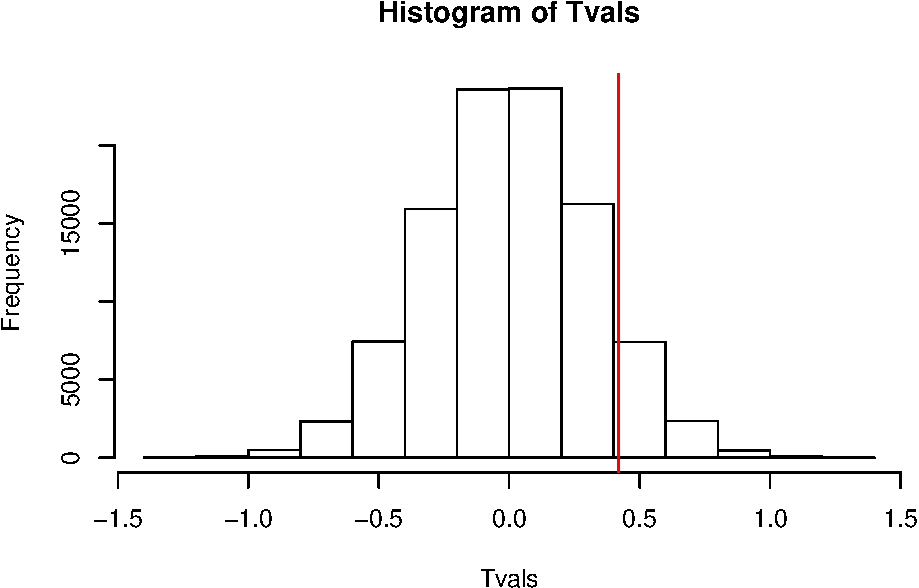
\includegraphics{03-pca_files/figure-latex/unnamed-chunk-4-1.pdf}

We can now compute the PC scores using
\begin{eqnarray*}
y_{i1} &=& \boldsymbol q_1^\top (\boldsymbol x_i - \bar{\boldsymbol x}) = 0.690 (x_{1i} - \bar{x}_1) + 0.724 (x_{2i} - \bar{x}_2) \\
y_{i2} &=& \boldsymbol q_2^\top (\boldsymbol x_i - \bar{\boldsymbol x}) = -0.724 (x_{1i} - \bar{x}_1) + 0.690 (x_{2i} - \bar{x}_2),
\end{eqnarray*}
which gives

FIX FIX

\begin{tabular}{l|rrrrrrrrrr}
Student & 1 & 2 & 3 & 4 & 5 & 6 & 7 & 8 & 9 & 10 \\ \hline
$y_{[1]}^\top$ & 19.1 & 16.2 & 11.6 & -14.7 & -23.1 & -14.9 & 3.8 & 30.0 & -15.3 & -12.6 \\
$y_{[2]}^\top$ & -7.3 & -7.2 & 6.4 & -0.8 & 5.1 & -9.3 & 4.4 & 5.9 & 4.2 & -1.5
\end{tabular}

Note that these new variables have sample mean \(\bar{\boldsymbol y}=\boldsymbol 0\) and sample covariance matrix (see part 4. of Proposition \ref{prp:pca1})
\[
\boldsymbol \Lambda= \text{diag}(\lambda_1,\lambda_2) =  \begin{pmatrix} 304.24 & 0 \\ 0 & 33.16 \end{pmatrix}.
\]
The plot below shows the PC scores \((y_{i1},y_{i2})^\top\). The two lines shown have lengths \(2\sqrt{\lambda_j}\), \(j=1,2\). Note that \(\sqrt{\lambda_j}\) is the standard deviation of the \(j\)th PC.

\begin{center}
\includegraphics[width=12cm,angle=0]{figs/prbsta_pca2.pdf}
\end{center}

Sometimes the new variables have an obvious interpretation. Note that the first PC gives positive, roughly equal, weight to PRB and STA and thus represents some form of ``average'' mark. For example, a student that has a high mark on PRB and STA will have a high value for \(y_1\). The second PC, meanwhile, represents a contrast between PRB and STA. For example, a large positive value for \(y_2\) implies the student did much better on STA than PRB, and a large negative value implies the opposite.

Note that we could have chosen \(t=-0.724\) instead of \(t=+0.724\). The only difference would be that the first eigenvector was \(\boldsymbol q_1^\ast = -\boldsymbol q_1\). In this case, a student who scored a high mark on PRB and STA would have a low value for \(y_1\). This is perfectly legitimate but makes the interpretation less intuitive. One can always change the sign of the eigenvectors if it makes interpretation easier.
```

\hypertarget{properties-of-principal-components}{%
\section{Properties of principal components}\label{properties-of-principal-components}}

Let \(\boldsymbol x_1, \ldots, \boldsymbol x_n\) have sample mean \(\bar{\boldsymbol x}\) and sample covariance matrix \(\boldsymbol S\), with spectral decomposition \(\boldsymbol S=\boldsymbol Q\boldsymbol \Lambda\boldsymbol Q^\top\) where
\(\boldsymbol Q=[\boldsymbol q_1, \ldots , \boldsymbol q_p]\) is orthogonal and \(\boldsymbol \Lambda=\text{diag}\{\lambda_1, \ldots , \lambda_p\}\). The transformed variables have some important properties.
\vskip 0.2truein

\begin{proposition}
\protect\hypertarget{prp:pca2}{}{\label{prp:pca2} }For \(j,k=1, \ldots , p\), the following results hold.

\begin{enumerate}
\def\labelenumi{\arabic{enumi}.}
\tightlist
\item
  \(\bar{y}_{+j} = n^{-1} \sum_{i=1}^n y_{ij}=n^{-1}\sum_{i=1}^n \boldsymbol q_j^\top (\boldsymbol x_i-\bar{\boldsymbol x})=0\);
\item
  \(\boldsymbol q_j^\top \boldsymbol S\boldsymbol q_j = \lambda_j\);
\item
  \(\boldsymbol q_j^\top \boldsymbol S\boldsymbol q_k = 0\) for \(j \neq k\);
\item
  \(\boldsymbol q_1^\top \boldsymbol S\boldsymbol q_1 \geq \boldsymbol q_2^\top \boldsymbol S\boldsymbol q_2 \geq \ldots \geq \boldsymbol q_p^\top \boldsymbol S\boldsymbol q_p\geq 0\);
\item
  \(\sum_{j=1}^p \boldsymbol q_j^\top \boldsymbol S\boldsymbol q_j = \sum_{j=1}^p \lambda_j = \text{tr}(\boldsymbol S)\);
\item
  \(\prod_{j=1}^p \boldsymbol q_j^\top \boldsymbol S\boldsymbol q_j = \prod_{j=1}^p \lambda_j = |\boldsymbol S|\).
\end{enumerate}
\end{proposition}

In words:

\begin{itemize}
\item
  part 1. tells us that the sample mean of \(y_{1j}, \ldots , y_{nj}\) for each fixed \(j\) is \(0\);
\item
  part 2. tells us that, for each fixed \(j\), the sample variance of
  the \(y_{ij},\, i=1, \ldots , n\) is \(\lambda_j\);
\item
  part 3. states that the sample covariance of the pairs \((y_{ij}, y_{ik})\), \(i=1, \ldots , n\), is \(0\) if \(j \neq k\);
\item
  part 4. states that the sample variance of \(y_{ij}, \, i=1, \ldots , n\), is not less than the sample variance of \(y_{ik}, \, i=1, \ldots , n\), if \(j\leq k\);
\item
  part 5. states that the sum of the sample variances is equal to the trace of \(\boldsymbol S\);
\item
  and part 6. states that the product of the sample variances is equal to the determinant of \(\boldsymbol S\).
\end{itemize}

From these properties we say that a proportion
\[\frac{\lambda_j}{\lambda_1 + \ldots + \lambda_p}\]
of the variability in the sample is `explained' by the \(j\)th PC.

For the G11PRB and G11STA data above,
\[\frac{\lambda_1}{\lambda_1 + \lambda_2} = \frac{304.24}{304.24+33.16} = 0.90,\]
so 90\% of the variability in the sample is explained by the 1st PC.

```\{Example\} We can apply PCA to a football league table where \(W\), \(D\), \(L\) are the number of matches won, drawn and lost and \(F\) and \(A\) are the goals scored for and against. An extract of the table for a recent Premiership season is:
FIX FIX

\begin{tabular}{lrrrrr}
\toprule
Team & W & D & L & F & A\\
\midrule
Chelsea & 27 & 5 & 6 & 103 & 32\\
Manchester United & 27 & 4 & 7 & 86 & 28\\
Arsenal & 23 & 6 & 9 & 83 & 41\\
Tottenham Hotspur & 21 & 7 & 10 & 67 & 41\\
Manchester City & 18 & 13 & 7 & 73 & 45\\
\bottomrule
\end{tabular}

The sample mean vector is

\[\bar{\boldsymbol x} =\begin{pmatrix}14.2 \\9.6 \\14.2 \\52.6 \\52.6 \\\end{pmatrix}\]

and the sample covariance matrix is

\begin{equation}
\boldsymbol S= \begin{pmatrix}39.4&-8.27&-31.1&116&-81.9 \\-8.27&8.14&0.13&-29.4&6.01 \\-31.1&0.13&31&-86.3&75.9 \\116&-29.4&-86.3&392&-209 \\-81.9&6.01&75.9&-209&231 \\\end{pmatrix}
\label{eq:PLES}
\end{equation}

The eigenvalues of \(\boldsymbol S\) are
\[\boldsymbol \Lambda= \text{diag}\begin{pmatrix}631&96.7&8.83&2.44&-4.97e-14 \\\end{pmatrix}\]

Note that we have a zero eigenvalue because one of our variables is a linear combination of the other variables, \(L = 38 - W - D\). The corresponding eigenvectors are
\[\boldsymbol Q= [\boldsymbol q_1 \ldots \boldsymbol q_5] =\begin{pmatrix}0.251&-0.0133&-0.116&0.768&0.577 \\-0.0477&-0.146&0.74&-0.309&0.577 \\-0.204&0.16&-0.624&-0.459&0.577 \\0.776&0.582&0.0674&-0.234&-2e-15 \\-0.539&0.784&0.213&0.222&1.83e-15 \\\end{pmatrix}\]

The proportion of variability explained by each of the PCs is:
\[
\begin{pmatrix}0.854&0.131&0.012&0.0033&-6.73e-17 \\\end{pmatrix}
\]

There is no point computing the scores for PC 5 because PC5 does not explain any of the variability in the data. Similarly, there is little value in computing the scores for PCs 3 \& 4 because they only account for 1.5\% of the variability in the data.

We can, therefore, choose to compute only the first two PC scores. We are reducing the dimension of our data set from \(p=5\) to \(p=2\) while still retaining 98.5\% of the variability. The first PC is given by:
\begin{align*}
y_{i1} &= 0.25(W_i-\bar{W}) +-0.05(D_i-\bar{D}) +-0.2(L_i-\bar{L})\\
& \qquad +0.78(F_i-\bar{F}) +-0.54(A_i-\bar{A}),
\end{align*}
and similarly for PC 2.

The first five rows of our revised ``league table'' are now

\begin{table}[H]
\centering
\begin{tabular}{lrr}
\toprule
Team & PC1 & PC2\\
\midrule
Chelsea & 55.3 & 12.3\\
Manchester United & 44.1 & -0.4\\
Arsenal & 33.3 & 8.1\\
Tottenham Hotspur & 20.1 & -1.2\\
Manchester City & 22.2 & 4.1\\
\bottomrule
\end{tabular}
\end{table}

Now that we have reduced the dimension to \(p=2\), we can visualise the differences between the teams.

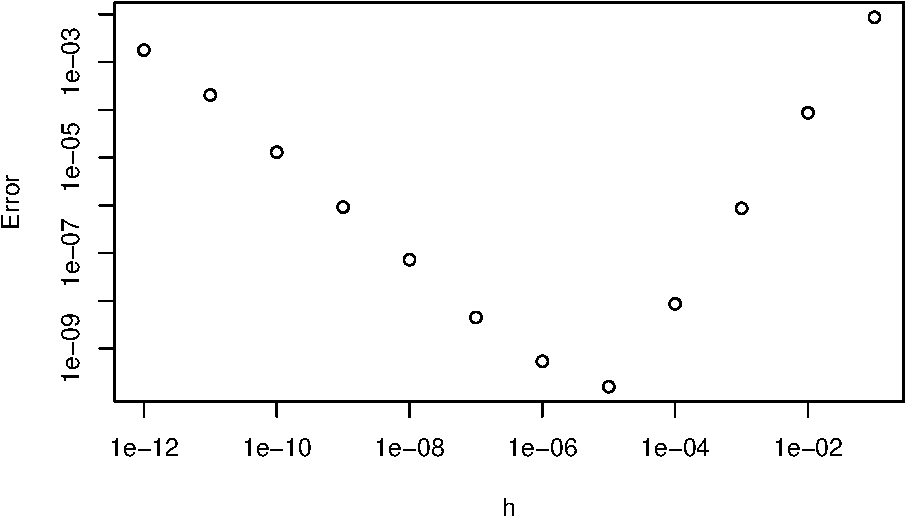
\includegraphics{03-pca_files/figure-latex/unnamed-chunk-8-1.pdf}

We might interpret the PCs as follows. The first PC seems to measure overall performance. It rewards teams with 0.78 for every goal they score and 0.25 for every match they win, while penalising them by 0.54 for every goal they concede, 0.2 for every match they lose and 0.05 for every match they draw.

We could, therefore, rank teams by PC 1 and compare this with the rankings using 3 points for a win and 1 point for a draw. The rankings are the same for the top three teams but differ below that. Under our system Wigan would be relegated in place of Portsmouth.

The second PC has a strong negative loading for both goals for and against. A team with a large negative PC 2 score was, therefore, involved in matches with lots of goals. We could, therefore, interpret PC 2 as an ``entertainment'' measure, ranking teams according to their involvement in high-scoring games.

The above example raises the question of how many PCs should we use in practice. If we reduce the dimension to \(p=1\) then we can rank observations and analyse our new variable with univariate statistics. If we reduce the dimension to \(p=2\) then it is still easy to visualise the data. However, reducing the dimension to \(p=1\) or \(p=2\) may involve losing lots of information and a sensible answer should depend on the objectives of the analysis and the data itself.

One tool for looking at the contributions of each PC is to look at the \textbf{scree graph} which plots the percentage of variance explained by PC \(j\) against \(j\). The scree graph for the football example is:

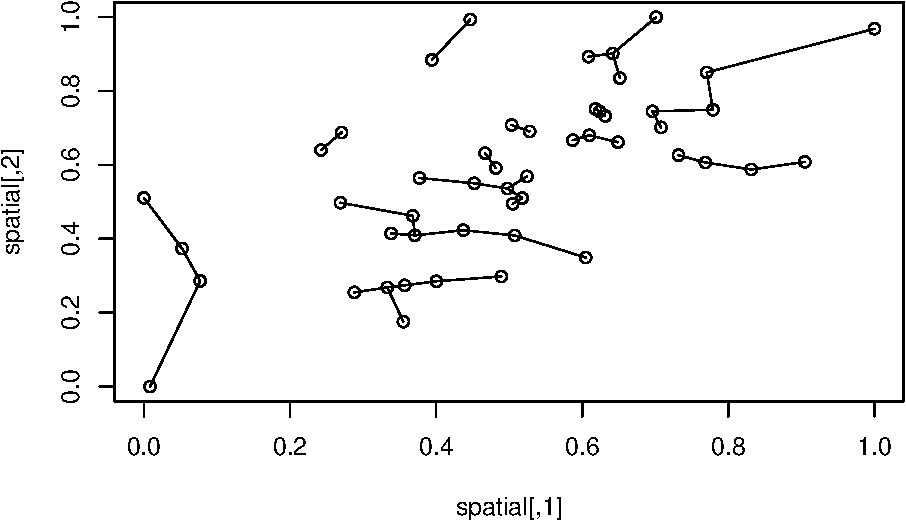
\includegraphics{03-pca_files/figure-latex/unnamed-chunk-9-1.pdf}

Possible methods for choosing the number of PCs include:

\begin{itemize}
\tightlist
\item
  retain enough PCs to explain, say, 90\% of the total variation;
\item
  retain PCs where the eigenvalue is above the average.
\end{itemize}

For the football example, the first method would retain 2 PCs whereas the second method would only retain 1 PC.

```

\hypertarget{population-pca}{%
\section{Population PCA}\label{population-pca}}

So far we have considered sample PCA based on the sample covariance matrix
\[
\boldsymbol S=\frac{1}{n}\sum_{i=1}^n (\boldsymbol x_i-\bar{\boldsymbol x})(\boldsymbol x_i-\bar{\boldsymbol x})^\top.
\]

We note now that there is a \emph{population} analogue of PCA based on the population
covariance matrix \(\boldsymbol \Sigma\). Although the population version of PCA is not of as much direct practical
relevance as sample PCA, it is nevertheless of conceptual importance.

Let \(\boldsymbol x\) denote a \(p \times 1\) random vector with \(E(\boldsymbol x)={\pmb \mu}\) and \(\text{Var}(\boldsymbol x)={\pmb \Sigma}\). As defined,
\(\pmb \mu\) is the population mean vector and \(\pmb \Sigma\) is the population covariance matrix.

Since \(\pmb \Sigma\) is symmetric, the spectral decomposition theorem tells us that
\[
{\pmb \Sigma}=\sum_{j=1}^p \check{\lambda}_j \check{\boldsymbol q}_j \check{\boldsymbol q}_j^\top=\check{\boldsymbol Q} \check{\boldsymbol \Lambda}\check{\boldsymbol Q}^\top
\]
where the `check' symbol \(\quad \check{} \quad\) is used to distinguish population quantities from their sample analogues.

Then:

\begin{itemize}
\tightlist
\item
  the first population PC is defined by \(Y_1=\check{\boldsymbol q}_1^\top (\boldsymbol x-{\pmb \mu})\);
  -the second population PC is defined by \(Y_2=\check{\boldsymbol q}_2^\top (\boldsymbol x-{\pmb \mu})\);
\item
  \$ldots\$
\item
  the \(p\)th population PC is defined by \(Y_p=\check{\boldsymbol q}_p^\top (\boldsymbol x-{\pmb \mu})\).
\end{itemize}

The \(Y_1, \ldots , Y_p\) are random variables, unlike the sample PCA case, where the \(y_{ij}\) are observed quantities.
In the sample PCA case, the \(y_{ij}\) can often be regarded as the observed values of random variables.

In matrix form, the above definitions can be summarised by writing
\[
\boldsymbol y=\begin{pmatrix} Y_1 \\ Y_2 \\ ... \\...\\Y_p   \end{pmatrix} = \check{\boldsymbol Q}^\top (\boldsymbol x-{\pmb \mu}).
\]

The population PCA analogues of the 6 sample PCA properties listed in Proposition \ref{prp:pca2} are now given. Note that the
\(Y_j\)'s are random variables as opposed to observed values of random variables.

\begin{proposition}
\protect\hypertarget{prp:pca3}{}{\label{prp:pca3} }The following results hold for the random variables \(Y_1, \ldots , Y_p\) defined above.

\begin{enumerate}
\def\labelenumi{\arabic{enumi}.}
\item
  \(E(Y_j)=0\) for \(j=1, \ldots , p\);\textbackslash{}
\item
  \(\text{Var}(Y_j)=\check{\lambda}_j\) for \(j=1,\ldots, p\);\textbackslash{}
\item
  \(\text{Cov}(Y_j,Y_k)=0\) if \(j \neq k\);\textbackslash{}
\item
  \(\text{Var}(Y_1) \geq \text{Var}(Y_2) \geq \cdots \geq \text{Var}(Y_p) \geq 0\);\textbackslash{}
\item
  \(\sum_{j=1}^p \text{Var}(Y_j)=\sum_{j=1}^p \check{\lambda}_j=\text{tr}(\boldsymbol \Sigma)\);\textbackslash{}
\item
  \(\prod_{j=1}^p \text{Var}(Y_j)=\prod_{j=1}^p \check{\lambda}_j=\vert \boldsymbol \Sigma\vert\).
\end{enumerate}
\end{proposition}

Note that, defining \(\boldsymbol y=(Y_1, \ldots , Y_p)^\top\) as before, part 1. implies that \(E(\boldsymbol y)={\mathbf 0}_p\) and parts 2. and 3. together imply that
\[
\text{Var}(\boldsymbol y)=\boldsymbol \Lambda\equiv \text{diag}(\check{\lambda}_1, \ldots , \check{\lambda}_p).
\]

\begin{example}
\protect\hypertarget{exm:unnamed-chunk-10}{}{\label{exm:unnamed-chunk-10} }Suppose
\[
\boldsymbol \Sigma=\boldsymbol I_p+ \delta {\mathbf 1}_p {\mathbf 1}_p^\top,
\]
where \(\delta>0\). What is the proportion of variability explained by the first PC? Since \(\delta>0\), the largest eigenvalue is \(\lambda_1=1+p\delta\) which is achieved when \(\check{\boldsymbol q}_1\) is the unit vector \(p^{-1/2}{\mathbf 1 }_p\). This and related examples are dealt with in more detail in the example sheets.
\end{example}

Consider now a repeated sampling framework in which we assume that \(\boldsymbol x_1, \ldots , \boldsymbol x_n\) are IID random vectors from a population
with mean vector \(\pmb \mu\) and covariance matrix \(\boldsymbol \Sigma\).

What is the relationship between the sample PCA based on the sample of observed vectors \(\boldsymbol x_1, \ldots , \boldsymbol x_n\), and the population PCA based on the unobserved random vector \(\boldsymbol x\),
from the same population?

Assuming \(n\) is large, and the elements of \(\boldsymbol \Sigma\) are all finite, the elements of the sample covariance matrix \(\boldsymbol S\) will be close with high probability to the corresponding elements
of the population covariance matrix \(\boldsymbol \Sigma\). Justification of this statement comes from the weak law of large numbers applied to the components of \(\Sigma\) (details omitted).

Consequently, when \(n\) is large, sample PCA and the corresponding population PCA may be expected to give similar results.

\hypertarget{an-alternative-derivation-of-pca}{%
\section{An Alternative Derivation of PCA}\label{an-alternative-derivation-of-pca}}

Consider a sample \(\boldsymbol x_1, \ldots , \boldsymbol x_n \in \mathbb{R}^p\).

Recall from \S2.8 that any line in \(\mathbb{R}^p\) may be written in the form
\(\{\boldsymbol a+u \boldsymbol b: \, u \in \mathbb{R}\}\) where \(\boldsymbol a, \boldsymbol b\in \mathbb{R}^p\) are
fixed.

Here we consider the following problem: \emph{find the best-fitting line to the sample}
\(\boldsymbol x_1, \ldots , \boldsymbol x_n\).

We first formulate this problem more precisely. Define the function
\begin{align*}
F(\boldsymbol a, \boldsymbol b; u_1, \ldots , u_n)&=\sum_{i=1}^n \vert \vert \boldsymbol x_i - \boldsymbol a- u_i \boldsymbol b\vert \vert^2\\
& =\sum_{i=1}^n (\boldsymbol x_i - \boldsymbol a-u_i \boldsymbol b)^\top (\boldsymbol x_i - \boldsymbol a-u_i \boldsymbol b).
\end{align*}

We wish to solve the following problem:
\begin{align}
&\textit{minimise $F(\boldsymbol a, \boldsymbol b; u_1, \ldots , u_n)$ subject to the}\nonumber \\
&\textit{constraints that $\boldsymbol a$ and $\boldsymbol b$ are orthogonal, i.e. $\boldsymbol a^\top \boldsymbol b=0$,}\label{eq:linemanager}\\
&\textit{and $\boldsymbol b$ is a unit vector, i.e. $\vert \vert \boldsymbol b\vert \vert =1$.} \nonumber
\end{align}

\begin{theorem}
\protect\hypertarget{thm:unnamed-chunk-11}{}{\label{thm:unnamed-chunk-11} }The solution to optimisation problem \eqref{eq:linemanager}
is given by
\begin{equation}
\hat{\boldsymbol a}=\left ({\mathbf I}_p-\boldsymbol q_1 \boldsymbol q_1^\top\right)\bar{\boldsymbol x}, \quad \hat{\boldsymbol b}= \boldsymbol q_1 \quad
\hbox{and} \quad \hat{u}_i=\boldsymbol x_i^\top \boldsymbol q_1, \quad i=1,\ldots , n,
\label{eq:hatitems}
\end{equation}
where \(\bar{\boldsymbol x}=n^{-1}\sum_{i=1}^n \boldsymbol x_i\) is the sample mean and the unit vector \(\boldsymbol q_1\) is the direction of the first sample PC.
\end{theorem}

Note that the quantities \(u_i -\bar{u}=\boldsymbol q_1^\top (\boldsymbol x_i-\bar{\boldsymbol x})\) are the PC scores associated with the first PC.

\begin{proof}
\iffalse{} {Proof. } \fi{}The proof is broken into two steps.

\textbf{Step 1}. In Step 1, we want to minimise \(F(\boldsymbol a, \boldsymbol b; u_1,\ldots, u_n)\) subject to the constraint \(\boldsymbol a^\top \boldsymbol b=0\), with \(\boldsymbol b\) an arbitrary \emph{fixed} unit vector in \(\mathbb{R}^p\). So we introduce a Lagrangian term for the constraint \(\boldsymbol a^\top \boldsymbol b=0\) and minimise
\[
\bar{F}(\boldsymbol a; u_1,\ldots ,  u_n; \gamma)
 \equiv \left \{\sum_{i=1}^n (\boldsymbol x_i -\boldsymbol a-u_i\boldsymbol b)^\top
(\boldsymbol x_i-\boldsymbol a-u_i\boldsymbol b)\right \}+ \gamma \boldsymbol a^\top \boldsymbol b
\]
over \(\boldsymbol a\), \(u_1, \ldots , u_n\) and \(\gamma\). Then, for \(i=1, \ldots , n\),
\begin{equation}
\frac{\partial \bar{F}}{\partial u_i}=-2\boldsymbol b^\top (\boldsymbol x_i-\boldsymbol a-u_i\boldsymbol b);
\label{eq:barF1}
\end{equation}
\begin{align}
\frac{\partial \bar{F}}{\partial \boldsymbol a}&=-2\left \{\sum_{i=1}^n (\boldsymbol x_i -\boldsymbol a-u_i\boldsymbol b)\right \}+\gamma \boldsymbol b\nonumber\\
&=-2n\{\bar{\boldsymbol x}-\boldsymbol a-(\bar{u}+\gamma/(2n))\boldsymbol b\},
\label{eq:barF2}
\end{align}
where \(\bar{u}=n^{-1}\sum_{i=1}^n u_i\); and
\begin{equation}
\frac{\partial \bar{F}}{\partial \gamma}=\boldsymbol a^\top \boldsymbol b.
\label{eq:barF3}
\end{equation}
Setting the partial derivatives \eqref{eq:barF1}, \eqref{eq:barF2} and @ref(eq:barF3\}) to zero,
\[
\frac{\partial \bar{F}}{\partial \gamma} =0 \implies \hat{\boldsymbol a}^\top \boldsymbol b=0;
\]
\begin{equation}
\frac{\partial \bar{F}}{\partial u_i}=0 \implies \hat{u}_i=\boldsymbol b^\top \boldsymbol x_i,
\label{eq:uhat}
\end{equation}
and therefore
\begin{equation}
\bar{\hat{u}}\equiv n^{-1} \sum_{i=1}^n \hat{u}_i=\boldsymbol b^\top \bar{\boldsymbol x};
\label{eq:barlambda}
\end{equation}
and
\[
\frac{\partial \bar{F}}{\partial \boldsymbol a}={\mathbf 0}_p \implies \hat{\boldsymbol a}=\bar{\boldsymbol x}-\{\bar{\hat{u}}+\hat{\gamma}/(2n)\}\boldsymbol b.
\]
Using \eqref{eq:barlambda} and the fact that \(\boldsymbol b^\top \hat{\boldsymbol a}=0\), it follows that
\[
0=\boldsymbol b^\top \hat{\boldsymbol a} =\boldsymbol b^\top [\bar{\boldsymbol x}-\{\hat{\bar{u}}+\hat{\gamma}/(2n)\}\boldsymbol b]=\boldsymbol b^\top \bar{\boldsymbol x}-\boldsymbol b^\top \bar{\boldsymbol x}
+\hat{\gamma}/(2n),
\]
which implies that \(\hat{\gamma}=0\). Consequently,
\begin{equation}
\hat{\boldsymbol a}=\bar{\boldsymbol x}-\bar{\hat{u}}\boldsymbol b=\bar{\boldsymbol x}-\boldsymbol b\boldsymbol b^\top \bar{\boldsymbol x}=\left ( \boldsymbol I_p-\boldsymbol b\boldsymbol b^\top \right ) \bar{\boldsymbol x};
\label{eq:bahat}
\end{equation}
and so
\begin{align}
&\bar{F}(\hat{\boldsymbol a}; \hat{u}_1, \ldots, \hat{u}_n; \hat{\gamma})\\
&=\sum_{i=1}^n (\boldsymbol x_i-\hat{\boldsymbol a}-\hat{u_i} \boldsymbol b)^\top (\boldsymbol x_i -\hat{\boldsymbol a}-\hat{u}_i\boldsymbol b)\nonumber \\
&=\sum_{i=1}^n \left \{\boldsymbol x_i-({\mathbf I}_p-\boldsymbol b\boldsymbol b^\top)\bar{\boldsymbol x}- \boldsymbol b\boldsymbol b^\top \boldsymbol x_i \right \}^\top \left \{\boldsymbol x_i -({\mathbf I}_p-\boldsymbol b\boldsymbol b^\top)\bar{\boldsymbol x} -\boldsymbol b\boldsymbol b^\top \boldsymbol x_i\right \}\nonumber \\
&\sum_{i=1}^n (\boldsymbol x_i -\bar{\boldsymbol x})^\top ({\mathbf I}_p -\boldsymbol b\boldsymbol b^\top)^2 (\boldsymbol x_i -\bar{\boldsymbol x})\nonumber \\
&= n \text{tr}\left \{ ({\mathbf I}_p-\boldsymbol b\boldsymbol b^\top )\boldsymbol S\right \} \nonumber \\
&=n\left \{\text{tr}(\boldsymbol S)-\boldsymbol b^\top \boldsymbol S\boldsymbol b\right\},
\label{eq:object37}
\end{align}
where \(\boldsymbol S\) is the sample covariance of the \(\boldsymbol x_i\).

\textbf{Step 2.} We now minimise \eqref{eq:object37} over unit vectors \(\boldsymbol b\in \mathbb{R}^p\). But minimising \eqref{eq:object37} is equivalent to maximising \(\boldsymbol b^\top \boldsymbol S\boldsymbol b\), so
from Proposition \ref{prp:two8}, \(\hat{\boldsymbol b}= \boldsymbol q_1\), and so \(\hat{\boldsymbol a}=(\boldsymbol I_p-\boldsymbol q_1 \boldsymbol q_1^\top)\bar{\boldsymbol x}\) from \eqref{eq:bahat}, and
from \eqref{eq:uhat}, \(\hat{u}_i=\boldsymbol q_1^\top \boldsymbol x_i\), \(i=1,\ldots , n\), all of which agrees with the expressions in \eqref{eq:hatitems}.\\
\end{proof}

\hypertarget{pca-under-transformations-of-variables}{%
\section{PCA under transformations of variables}\label{pca-under-transformations-of-variables}}

Let us return to the example of \(n=10\) students who studied G11PRB and G11STA. Earlier, we calculated the sample mean, sample variance matrix and the eigenvalues/vectors of \(\boldsymbol S\),
\begin{eqnarray*}
\bar{\boldsymbol x} = \begin{pmatrix} 62.6 \\ 66.2 \end{pmatrix}, &\quad&
\boldsymbol S= \begin{pmatrix} 162.04 & 135.38 \\ 135.38 & 175.36 \end{pmatrix} \\
\boldsymbol \Lambda= \begin{pmatrix} 304.24 & 0 \\ 0 & 33.16 \end{pmatrix}, &\quad&
\boldsymbol Q= \begin{pmatrix} 0.690 & -0.724 \\ 0.724 & 0.690 \end{pmatrix}
\end{eqnarray*}
with PC 1 scores
\[y_i = \boldsymbol q_1^\top (\boldsymbol x_i - \bar{\boldsymbol x}) = 0.690 (x_{1i} - \bar{x}_1) + 0.724 (x_{2i} - \bar{x}_2).\]

We now consider what happens to the above quantities under various transformations of the \(\boldsymbol x_i\), the \(2 \times 1\)
response vectors.

\textbf{Addition transformation}

Firstly, we consider the transformation of addition where, for example, the G11PRB lecturer decides to add 5 marks for all the students. We can write this transformation as \(\boldsymbol z_i = \boldsymbol x_i + \boldsymbol c\), where \(\boldsymbol c\) is a fixed vector. Under this transformation the sample mean changes, \(\bar{\boldsymbol z} = \bar{\boldsymbol x} + \boldsymbol c\), but the sample variance remains \(\boldsymbol S\). Consequently, the eigenvalues and eigenvectors of \(\boldsymbol S\) remain the same and, therefore, so does the PC 1 score,
\[y_i = \boldsymbol q_1^\top (\boldsymbol z_i - \bar{\boldsymbol z}) = \boldsymbol q_1^\top(\boldsymbol x_i + \boldsymbol c- (\bar{\boldsymbol x} + \boldsymbol c)) = \boldsymbol q_1^\top (\boldsymbol x_i - \bar{\boldsymbol x}).\]
We say that the principal components are \textbf{invariant} under the addition transformation. An important special case is to choose \(\boldsymbol c= -\bar{\boldsymbol x}\) so that the PC 1 score is simply \(y_i = \boldsymbol q_1^\top \boldsymbol z_i\).

\textbf{Scale transformation}

Secondly, we consider the scale transformation where, for example, the G11PRB lecturer decides to double the marks for all students. A scale transformation occurs more naturally when we convert units of measurement from, say, metres to kilometres. We can write this transformation as \(\boldsymbol z_i = \boldsymbol D\boldsymbol x_i\), where \(\boldsymbol D\) is a diagonal matrix with positive elements. Under this transformation the sample mean changes from \(\bar{\boldsymbol x}\) to \(\bar{\boldsymbol z} = \boldsymbol D\bar{\boldsymbol x}\), and the sample covariance matrix changes from \(\boldsymbol S\) to \(\boldsymbol D\boldsymbol S\boldsymbol D\). Consequently, the principal components also change.

This lack of scale-invariance is undesirable. One solution is to choose
\[
\boldsymbol D= \text{diag}(s_{11}^{-1/2}, \ldots , s_{pp}^{-1/2}),
 \]
where \(s_{ii}\) is the \(i\)th diagonal element of \(\boldsymbol S\). In effect, we have standardised all the new variables to have variance 1. In this case the sample covariance matrix of the \(\boldsymbol z_i\)'s is simply the sample correlation matrix of the original variables, \(\boldsymbol x_i\). Therefore, we can carry out PCA on the sample correlation matrix, \(\boldsymbol R\), which is invariant to changes of scale.

In summary: \(\boldsymbol R\) is scale-invariant while \(\boldsymbol S\) is not.

\begin{example}
\protect\hypertarget{exm:unnamed-chunk-13}{}{\label{exm:unnamed-chunk-13} }For the G11PRB/G11STA data, we choose
\[
\boldsymbol D= \text{diag}(162.04,175.36)^{-1/2} = \text{diag}(0.079,0.076)
\]
so that \(\boldsymbol z_i = \boldsymbol D\boldsymbol x_i\).
The sample correlation matrix is then
\begin{align*}
\boldsymbol R&= \boldsymbol D\boldsymbol S\boldsymbol D\\
 &= \begin{pmatrix} 0.079 & 0 \\ 0 & 0.076 \end{pmatrix}
\begin{pmatrix} 162.04 & 135.38 \\ 135.38 & 175.36 \end{pmatrix}
\begin{pmatrix} 0.079 & 0 \\ 0 & 0.076 \end{pmatrix} \\
&= \begin{pmatrix} 1.000 & 0.803 \\ 0.803 & 1.000 \end{pmatrix}.
\end{align*}
The eigenvalues and eigenvectors of \(\boldsymbol R\) are then
\[\boldsymbol \Lambda= \begin{pmatrix} 1.803 & 0 \\ 0 & 0.197 \end{pmatrix}, \qquad
\boldsymbol Q= \begin{pmatrix} 0.707 & 0.707 \\ 0.707 & -0.707 \end{pmatrix},\]
and the PC 1 score is
\begin{eqnarray*}
y_i &=& \boldsymbol q_1^\top (\boldsymbol z_i - \bar{\boldsymbol z}) = \boldsymbol q_1^\top \boldsymbol D(\boldsymbol x_i - \bar{\boldsymbol x}) \\
&=& 0.707 \times 0.079 (x_{1i} - \bar{x}_1) + 0.707 \times 0.076 (x_{2i} - \bar{x}_2).
\end{eqnarray*}

In the example above, there is little difference between using \(\boldsymbol S\) and \(\boldsymbol R\) for the PCA because the variances for G11PRB and G11STA are similar. In other cases, particularly when the variables are measured on wildly different scales, the difference will be notable. For example, in the football data the sample variances of \(F\) and \(A\) are much larger than the sample variances of \(W\), \(D\) and \(L\).
\end{example}

\textbf{Orthogonal transformation}

Thirdly, we consider a transformation by an orthogonal matrix, \(\stackrel{p \times p}{\boldsymbol A}\), such that \(\boldsymbol A\boldsymbol A^\top = \boldsymbol A^\top \boldsymbol A= \boldsymbol I_p\), and write \(\boldsymbol z_i = \boldsymbol A\boldsymbol x_i\). This is equivalent to rotating and/or reflecting the original data.

Let \(\boldsymbol S\) be the sample covariance matrix of the \(\boldsymbol x_i\) and let \(\boldsymbol T\) be the sample covariance matrix of the \(\boldsymbol z_i\). Under this transformation the sample mean changes from \(\bar{\boldsymbol x}\) to \(\bar{\boldsymbol z} = \boldsymbol A\bar{\boldsymbol x}\), and the sample covariance matrix \(\boldsymbol S\) changes from \(\boldsymbol S\) to \(\boldsymbol T= \boldsymbol A\boldsymbol S\boldsymbol A^\top\).

However, if we write \(\boldsymbol S\) in terms of its spectral decomposition \(\boldsymbol S= \boldsymbol Q\boldsymbol \Lambda\boldsymbol Q^\top\), then \(\boldsymbol T= \boldsymbol A\boldsymbol Q\boldsymbol \Lambda\boldsymbol Q^\top \boldsymbol A^\top = \boldsymbol B\boldsymbol \Lambda\boldsymbol B^\top\) where \(\boldsymbol B= \boldsymbol A\boldsymbol Q\) is also orthogonal. It is therefore apparent that the eigenvalues of \(\boldsymbol T\) are the same as those of \(\boldsymbol S\); and the eigenvectors of \(\boldsymbol T\) are given by \(\boldsymbol b_j\) where \(\boldsymbol b_j = \boldsymbol A\boldsymbol q_j\), \(j=1,\ldots,p\). The PC 1 scores of the transformed variables are
\[ y_i = \boldsymbol b_1^\top (\boldsymbol z_i - \bar{\boldsymbol z}) = \boldsymbol q_1^\top \boldsymbol A^\top \boldsymbol A(\boldsymbol x_i - \bar{\boldsymbol x}) = \boldsymbol q_1^\top (\boldsymbol x_i - \bar{\boldsymbol x}),\]
and so they are identical to the PC 1 scores of the original variables.

Therefore, under an orthogonal transformation the eigenvalues and PC scores are unchanged and the PCs are orthogonal transformations of the original PCs. We say that the principal components are \textbf{equivariant} with respect to orthogonal transformations.

\begin{example}
\protect\hypertarget{exm:unnamed-chunk-14}{}{\label{exm:unnamed-chunk-14} }Suppose we rotate the G11PRB/G11STA data by the matrix \(\boldsymbol A= \begin{pmatrix} 0.866 & -0.500 \\ 0.500 & 0.866 \end{pmatrix}\). The sample covariance matrix of the rotated data is
\begin{align*}
\boldsymbol T&= \boldsymbol A\boldsymbol S\boldsymbol A^\top\\
&= \begin{pmatrix} 0.866 & -0.500 \\ 0.500 & 0.866 \end{pmatrix}
\begin{pmatrix} 162.04 & 135.38 \\ 135.38 & 175.36 \end{pmatrix}
\begin{pmatrix} 0.866 & 0.500 \\ -0.500 & 0.866 \end{pmatrix} \\
&= \begin{pmatrix} 48.13 & 61.92 \\ 61.92 & 289.27 \end{pmatrix}.
\end{align*}
The eigenvalues of \(\boldsymbol T\) are \(304.24\) and \(33.16\) (same as for \(\boldsymbol S\)). The eigenvectors of \(\boldsymbol T\) are then
\begin{eqnarray*}
\boldsymbol B&=& \boldsymbol A\boldsymbol Q= \begin{pmatrix} 0.866 & -0.500 \\ 0.500 & 0.866 \end{pmatrix} \begin{pmatrix} 0.690 & -0.724 \\ 0.724 & 0.690 \end{pmatrix} \\
&=& \begin{pmatrix} 0.235 & -0.972 \\ 0.972 & 0.235 \end{pmatrix}
\end{eqnarray*}
and the PC 1 scores are unchanged.
\end{example}

\hypertarget{pca-based-on-boldsymbol-s-versus-pca-based-on-boldsymbol-r}{%
\section{\texorpdfstring{PCA based on \(\boldsymbol S\) versus PCA based on \(\boldsymbol R\)}{PCA based on \textbackslash{}boldsymbol S versus PCA based on \textbackslash{}boldsymbol R}}\label{pca-based-on-boldsymbol-s-versus-pca-based-on-boldsymbol-r}}

Recall the distinction between the sample covariance matrix \(\boldsymbol S\) and the sample correlation matrix \(\boldsymbol R\).

Note that all correlation matrices are also covariance matrices, but not all covariance matrices are correlation matrices.

So in practice we have a choice of using \(\boldsymbol S\) or \(\boldsymbol R\) for PCA. As we have seen, PCA based on \(\boldsymbol R\) is scale invariant, but PCA based on \(\boldsymbol S\) is not; while PCA based on \(\boldsymbol S\) is invariant (eigenvalues and PC scores) and equivariant (eigenvectors) under orthogonal transformation, whereas \(\boldsymbol R\) is not.

This raises the important practical question: for a given dataset, should we use PCA based on \(\boldsymbol S\) or \(\boldsymbol R\)?

If the \(p\) variables represent very different types of quantity or show marked differences in variances, then it will usually be better to use \(\boldsymbol R\) rather than \(\boldsymbol S\). However, in some circumstances, we may wish to use \(\boldsymbol S\), such as when the \(p\) variables are measuring similar entities and the sample variances are not too different.

Bearing in mind that the required numerical calculations are so easy to perform in R, we might wish to do it both ways and see if it makes much difference.

\hypertarget{cca}{%
\chapter{Canonical Correlation Analysis}\label{cca}}

Suppose we observe a random sample of \(n\) bivariate observations
\[
\boldsymbol z_1=(x_1,y_1)^\top , \ldots , \boldsymbol z_n=(x_n,y_n)^\top.
\]
If we are interested in exploring possible dependence between the \(x_i\)'s and \(y_i\)'s then among the first things we would do would be to obtain a scatterplot of the \(x_i\)'s against the \(y_i\)'s and calculate the correlation coefficient. Recall that the sample correlation coefficient is defined by
\begin{equation}
r=r[x,y]=\frac{n^{-1}\sum_{i=1}^n (x_i-\bar{x})(y_i-\bar{y})}{\left ( n^{-1}\sum_{i=1}^n (x_i-\bar{x})^2  \right )^{1/2}  \left ( n^{-1}\sum_{i=1}^n (y_i-\bar{y})^2 \right )^{1/2}}
\label{eq:scr}
\end{equation}
where \(\bar{x}=n^{-1}\sum_{i=1}^n x_i\) and \(\bar{y}=n^{-1}\sum_{i=1}^n y_i\) are the sample means. Note that the sample correlation is a \textbf{scale-free measure} of the strength of \textbf{linear dependence} between the \(x_i\)'s and the \(y_i\)'s.

In this chapter we investigate the multivariate analogue of this question. Suppose
\[
\boldsymbol z_i =(\boldsymbol x_i^\top,\boldsymbol y_i^\top)^\top, \qquad i=1,\ldots, n,
\]
is a random sample of vectors. What is a sensible way to assess and describe the strength of the linear dependence between the \(\boldsymbol x_i\) vectors and the \(\boldsymbol y_i\) vectors? That is what this chapter is about. A key role is played by the singular valued decomposition (SVD) introduced in Result 2.13 in Chapter 2.

\begin{example}
\protect\hypertarget{exm:prem}{}{\label{exm:prem} }From time to time we will return to the Premier League example in this chapter. We shall treat \(W\) and \(D\), the number of wins and draws, respectively, as the \(x\)-variables; and \(F\) and \(A\), the number of goals for and against, will be treated as the \(y\)-variables. The number of losses, \(L\), is omitted as it provides no additional information when we know \(W\) and \(D\). A question we shall consider is: how strongly associated are the match outcome variables, \(W\) and \(D\), with the goals for and against variables, \(F\) and \(A\)?
\end{example}

\hypertarget{canonical-correlation-analysis}{%
\section{Canonical Correlation Analysis}\label{canonical-correlation-analysis}}

Assume we are given a random sample of vectors
\[
\boldsymbol z_i=(\boldsymbol x_i^\top , \boldsymbol y_i^\top )^\top: \, i=1,\ldots, n,
\]
where
the \(\boldsymbol x_i\) are \(p \times 1\), the \(\boldsymbol y_i\) are \(q \times 1\) and, consequently, the \(\boldsymbol z_i\) are \((p+q)\times 1\). We are interested in determining the strength of linear association between the \(\boldsymbol x_i\) vectors and the \(\boldsymbol y_i\) vectors.

Write
\[
\bar{\boldsymbol z}=n^{-1}\sum_{i=1}^n \boldsymbol z_i, \qquad \bar{\boldsymbol x}=n^{-1} \sum_{i=1}^n \boldsymbol x_i \qquad \text{and} \qquad \bar{\boldsymbol y}=n^{-1}\sum_{i=1}^n \boldsymbol y_i
\]
for the sample mean vectors of the \(\boldsymbol z_i\), \(\boldsymbol x_i\) and \(\boldsymbol y_i\) respectively.

We formulate this task as an optimisation problem (cf.~PCA). First, we introduce some notation. Let \(\boldsymbol S_{\boldsymbol z\boldsymbol z}\) denote the sample covariance matrix of the \(\boldsymbol z_i\), \(i=1,\ldots, n\). Then \(\boldsymbol S_{\boldsymbol z\boldsymbol z}\) can be written in block matrix form
\[
\boldsymbol S_{\boldsymbol z\boldsymbol z}=\left [\begin{array}{cc}
\boldsymbol S_{\boldsymbol x\boldsymbol x} & \boldsymbol S_{\boldsymbol x\boldsymbol y}\\
\boldsymbol S_{\boldsymbol y\boldsymbol x} & \boldsymbol S_{\boldsymbol y\boldsymbol y} \end{array} \right ],
\]
where \(\boldsymbol S_{\boldsymbol x\boldsymbol x}\) (\(p \times p\)) is the sample covariance matrix of the \(\boldsymbol x_i\), \(\boldsymbol S_{\boldsymbol y\boldsymbol y}\) (\(q \times q\)) is the sample covariance of the \(\boldsymbol y_i\), and the cross-covariance matrices are given by
\[
\stackrel{p \times q}{\boldsymbol S}_{\boldsymbol x\boldsymbol y}=n^{-1} \sum_{i=1}^n (\boldsymbol x_i -\bar{\boldsymbol x})(\boldsymbol y_i-\bar{\boldsymbol y})^\top
\qquad \text{and} \qquad \stackrel{q \times p}{\boldsymbol S}_{\boldsymbol y\boldsymbol x}=\boldsymbol S_{\boldsymbol x\boldsymbol y}^\top.
\]

\textbf{Example \ref{exm:prem} (continued)}. The relevant covariance matrix here is given in \eqref{eq:PLES},
but we need to delete the middle row and middle column because this relates to the variable \(L\), the number of losses,
which we are omitting. So we are left with
\begin{equation}
\boldsymbol S_{\boldsymbol x\boldsymbol x}=\begin{pmatrix} 39.4 & -8.3\\ -8.3 & 8.1   \end{pmatrix} , \qquad
\boldsymbol S_{\boldsymbol y\boldsymbol y}=\begin{pmatrix} 392.2 & -208.7\\ -208.7 & 230.9   \end{pmatrix}
\label{eq:bSxy1}
\end{equation}
and
\begin{equation}
\boldsymbol S_{\boldsymbol x\boldsymbol y}=\boldsymbol S_{\boldsymbol y\boldsymbol x}^\top =
\begin{pmatrix} 115.7  & -81.9\\ -29.4 & 6.0   \end{pmatrix}.
\label{eq:bSxy2}
\end{equation}
We shall return to this example in a little while.

We want to find the linear combination of the \(x\)-variables and the linear combination of the \(y\)-variables which is most highly correlated.

One version of the optimisation problem we want to solve is: find non-zero vectors \(\stackrel{p \times 1}{\boldsymbol a}\) and \(\stackrel{q \times 1}{\boldsymbol b}\) which maximise the correlation coefficient
\[
r[\boldsymbol a^\top \boldsymbol x,\boldsymbol b^\top \boldsymbol y]=\frac{\boldsymbol a^\top \boldsymbol S_{\boldsymbol x\boldsymbol y}\boldsymbol b}{(\boldsymbol a^\top \boldsymbol S_{\boldsymbol x\boldsymbol x}\boldsymbol a)^{1/2}(\boldsymbol b^\top \boldsymbol S_{\boldsymbol y\boldsymbol y}\boldsymbol b)^{1/2}}.
\]
In other words:
\begin{align}
  &\mbox{Find non-zero vectors }\quad  \boldsymbol a\;\; (p \times 1)\mbox{ and  } \boldsymbol b\;\; (q \times 1) \nonumber\\
  &\mbox{to maximise} \qquad  r[\boldsymbol a^\top \boldsymbol x,\boldsymbol b^\top \boldsymbol y],
\label{eq:opt26}
\end{align}

where \(r[.,.]\) is defined in \eqref{eq:scr}.
Intuitively, this makes sense, because we want to find the linear combination of the \(x\)-variables and the linear combination of the \(y\)-variables which are most highly correlated.

However, note that for any \(\gamma>0\) and \(\delta>0\),
\begin{equation}
  r[\gamma\boldsymbol a^\top \boldsymbol x, \delta \boldsymbol b^\top \boldsymbol y]= \frac{\gamma \delta}{\sqrt{\gamma^2 \delta^2}}r[\boldsymbol a^\top \boldsymbol x,\boldsymbol b^\top \boldsymbol y]=r[\boldsymbol a^\top \boldsymbol x,\boldsymbol b^\top \boldsymbol y],
  \label{eq:invar}
  \end{equation}
i.e. \(r[\boldsymbol a^\top \boldsymbol x,\boldsymbol b^\top \boldsymbol y]\) is invariant with respect to positive scalar multiplication of \(\boldsymbol a\) and \(\boldsymbol b\). Consequently there will be an infinite number of solutions to this optimisation problem, because if \(\boldsymbol a\) and \(\boldsymbol b\) are solutions to optimization problem \eqref{eq:opt26}, then so are \(\gamma \boldsymbol a\) and \(\delta \boldsymbol b\), for any \(\gamma>0\) and \(\delta>0\).

A more useful way to formulate this optimisation problem is the following: find
\begin{equation}
\max_{\boldsymbol a, \boldsymbol b} \boldsymbol a^\top \boldsymbol S_{\boldsymbol x\boldsymbol y}\boldsymbol b
\label{eq:opt27a}
\end{equation}
subject to the constraints
\begin{equation}
\boldsymbol a^\top \boldsymbol S_{\boldsymbol x\boldsymbol x}\boldsymbol a=1 \qquad \text{and} \qquad \boldsymbol b^\top \boldsymbol S_{\boldsymbol y\boldsymbol y}\boldsymbol b=1.
\label{eq:opt27b}
\end{equation}

\begin{proposition}
\protect\hypertarget{prp:unnamed-chunk-1}{}{\label{prp:unnamed-chunk-1} }Assume that \(\boldsymbol S_{\boldsymbol x\boldsymbol x}\) and \(\boldsymbol S_{\boldsymbol y\boldsymbol y}\) both are non-singular. Then the following holds.

\begin{enumerate}
\def\labelenumi{\arabic{enumi}.}
\item
  If \(\boldsymbol a=\hat{\boldsymbol a}\) and \(\boldsymbol b=\hat{\boldsymbol b}\) maximise \eqref{eq:opt26}, then
  \[
  \boldsymbol a=\check{\boldsymbol a}\equiv\hat{\boldsymbol a}/(\hat{\boldsymbol a}^\top \boldsymbol S_{\boldsymbol x\boldsymbol x}\hat{\boldsymbol a})^{1/2} \qquad \text{and} \qquad
  \boldsymbol b=\check{\boldsymbol b}\equiv \hat{\boldsymbol b}/(\hat{\boldsymbol b}^\top \boldsymbol S_{\boldsymbol y\boldsymbol y}\hat{\boldsymbol b})^{1/2}
  \]
  maximise \eqref{eq:opt27a} subject to the constraints \eqref{eq:opt27b}. Moreover, if \(\boldsymbol a=\check{\boldsymbol a}\) and \(\boldsymbol b=\check{\boldsymbol b}\) maximise \eqref{eq:opt27a} subject to constraints
  \eqref{eq:opt27b} then, for any \(\gamma>0\) and \(\delta>0\), \(\boldsymbol a=\gamma \check{\boldsymbol a}\) and \(\boldsymbol b=\delta \check{\boldsymbol b}\) maximise \eqref{eq:opt26}.
\item
  The optimum solution to \eqref{eq:opt27a} and \eqref{eq:opt27b} is obtained when \(\boldsymbol a=\boldsymbol S_{\boldsymbol x\boldsymbol x}^{-1/2}{\mathbf q}_1\) and \(\boldsymbol b=\boldsymbol S_{\boldsymbol y\boldsymbol y}^{-1/2} {\mathbf r}_1\), where \(\boldsymbol S_{\boldsymbol x\boldsymbol x}^{-1/2} \boldsymbol S_{\boldsymbol x\boldsymbol y}\boldsymbol S_{\boldsymbol y\boldsymbol y}^{-1/2}\) has SVD
  \begin{equation}
  \boldsymbol A\equiv \boldsymbol S_{\boldsymbol x\boldsymbol x}^{-1/2}\boldsymbol S_{\boldsymbol x\boldsymbol y}\boldsymbol S_{\boldsymbol y\boldsymbol y}^{-1/2}= \sum_{j=1}^t \xi_j {\mathbf q}_j {\mathbf r}_j^\top \equiv {\mathbf Q}{\pmb \Xi} {\mathbf R}^\top,
  \label{eq:svdcca}
  \end{equation}
  where \(\boldsymbol A\) has rank \(t\) and \(\xi_1 \geq \cdots \geq \xi_t >0\).
\item
  The maximum value of the correlation coefficient is given by the largest singular value \(\xi_1\).
\end{enumerate}
\end{proposition}

Note: the matrix square roots \(\boldsymbol S_{\boldsymbol x\boldsymbol x}^{-1/2}\) and \(\boldsymbol S_{\boldsymbol y\boldsymbol y}^{-1/2}\) of \(\boldsymbol S_{\boldsymbol x\boldsymbol x}^{-1}\) and \(\boldsymbol S_{\boldsymbol y\boldsymbol y}^{-1}\), respectively, are defined using the definition of matrix square roots of symmetric non-negative definite matrices given in Chapter 2.

\begin{proof}
\iffalse{} {Proof. } \fi{}(i) In \eqref{eq:invar} it was noted that, for \(\boldsymbol a\neq {\mathbf 0}_p\) and \(\boldsymbol b\neq {\mathbf 0}_q\), the expression for \(r[\boldsymbol a^\top \boldsymbol x, \boldsymbol b^\top \boldsymbol y]\) is invariant when we change \(\boldsymbol a\) to \(\gamma \boldsymbol a\) and change \(\boldsymbol b\) to \(\delta \boldsymbol b\), where \(\gamma>0\) and \(\delta>0\) are scalars, so the second statement in Result 4.1(i) follows imnmdeiately. Suppose now a solution to problem \eqref{eq:opt26} is achieved when \(\boldsymbol a= \hat{\boldsymbol a}\) and \(\boldsymbol b=\hat{\boldsymbol b}\). Then, due to the invariance with respect to rescaling, the optimum is also achieved when \(\boldsymbol a=\check{\boldsymbol a}\equiv\hat{\boldsymbol a}/(\hat{\boldsymbol a}^\top \boldsymbol S_{\boldsymbol x\boldsymbol x} \hat{\boldsymbol a})^{1/2}\) and \(\boldsymbol b=\check{\boldsymbol b}\equiv \hat{\boldsymbol b}/(\hat{\boldsymbol b}^\top \boldsymbol S_{\boldsymbol y\boldsymbol y} \hat{\boldsymbol b})^{1/2}\). But by definition of \(\check{\boldsymbol a}\) and \(\check{\boldsymbol b}\), they satisfy the constraints \eqref{eq:opt27b} because
\[
\check{\boldsymbol a}^\top \boldsymbol S_{\boldsymbol x\boldsymbol x} \check{\boldsymbol a}=\frac{\hat{\boldsymbol a}^\top \boldsymbol S_{\boldsymbol x\boldsymbol x}\hat{\boldsymbol a}}{\left \{ \left (\hat{\boldsymbol a}^\top \boldsymbol S_{\boldsymbol x\boldsymbol x}\hat{\boldsymbol a}\right )^{1/2}\right \}^2}
=\frac{\hat{\boldsymbol a}^\top \boldsymbol S_{\boldsymbol x\boldsymbol x}\hat{\boldsymbol a}}{\hat{\boldsymbol a}^\top \boldsymbol S_{\boldsymbol x\boldsymbol x}\hat{\boldsymbol a}}=1
\]
and, similarly,
\[
\check{\boldsymbol b}^\top \boldsymbol S_{\boldsymbol y\boldsymbol y} \check{\boldsymbol b}=\frac{\hat{\boldsymbol b}^\top \boldsymbol S_{\boldsymbol y\boldsymbol y}\hat{\boldsymbol b}}{\hat{\boldsymbol b}^\top \boldsymbol S_{\boldsymbol y\boldsymbol y}\hat{\boldsymbol b}}=1.
\]
So \(\boldsymbol a=\check{\boldsymbol a}\) and \(\boldsymbol b=\check{\boldsymbol b}\) maximises \eqref{eq:opt27a} subject to the constraints \eqref{eq:opt27b}.

\noindent (ii) \& (iii) We may write the constraints \eqref{eq:opt27b} as
\[
\tilde{\boldsymbol a}^\top \tilde{\boldsymbol a}=1 \qquad \text{and} \qquad \tilde{\boldsymbol b}^\top \tilde{\boldsymbol b}=1
\]
where
\[
\tilde{\boldsymbol a}=\boldsymbol S_{\boldsymbol x\boldsymbol x}^{1/2} \boldsymbol a\qquad \text{and} \qquad \tilde{\boldsymbol b}=\boldsymbol S_{\boldsymbol y\boldsymbol y}^{1/2}\boldsymbol b.
\]

Recall that \(\boldsymbol S_{\boldsymbol x\boldsymbol x}\) and \(\boldsymbol S_{\boldsymbol y\boldsymbol y}\) are assumed to be non-singular. Then, using results from Chapter 2, \(\boldsymbol S_{\boldsymbol x\boldsymbol x}^{1/2}\) and \(\boldsymbol S_{\boldsymbol y\boldsymbol y}^{1/2}\) will also be non-singular, and so
\[
(\boldsymbol S_{\boldsymbol x\boldsymbol x}^{1/2})^{-1}=\boldsymbol S_{\boldsymbol x\boldsymbol x}^{-1/2} \qquad \text{and} \qquad (\boldsymbol S_{\boldsymbol y\boldsymbol y}^{1/2})^{-1}=\boldsymbol S_{\boldsymbol y\boldsymbol y}^{-1/2}
\]
both exist and so we may write
\[
\boldsymbol a=\boldsymbol S_{\boldsymbol x\boldsymbol x}^{-1/2}\tilde{\boldsymbol a} \qquad \text{and} \qquad \boldsymbol b=\boldsymbol S_{\boldsymbol y\boldsymbol y}^{-1/2} \tilde{\boldsymbol b},
\]
and optimisation problem \eqref{eq:opt27a} subject to \eqref{eq:opt27b} becomes
\[
\max_{\tilde{\boldsymbol a}, \tilde{\boldsymbol b}}
\tilde{\boldsymbol a}^\top \boldsymbol S_{\boldsymbol x\boldsymbol x}^{-1/2}\boldsymbol S_{\boldsymbol x\boldsymbol y}\boldsymbol S_{\boldsymbol y\boldsymbol y}^{-1/2} \tilde{\boldsymbol b}
\]
subject to
\[
\vert \vert \tilde{\boldsymbol a} \vert \vert =1 \qquad \text{and} \qquad \vert \vert \tilde{\boldsymbol b}\vert \vert=1.
\]
From the properties of the SVD, and in particular Result 2.15 in Chapter 2, we know that the maximum correlation is \(\xi_1\). Moreover, using the SVD again, this is achieved when \(\tilde{\boldsymbol a}={\mathbf q}_1\) and \(\tilde{\boldsymbol b}={\mathbf r}_1\) or, equivalently, \(\boldsymbol a=\boldsymbol S_{\boldsymbol x\boldsymbol x}^{-1/2}{\mathbf q}_1\) and \(\boldsymbol b=\boldsymbol S_{\boldsymbol y\boldsymbol y}^{-1/2}{\mathbf r}_1\).\\
\end{proof}

\textbf{Example \ref{exm:prem} (continued)}
We now want to calculate the matrix \(\boldsymbol A\) in \eqref{eq:svdcca} and then find its singular valued decomposition. We first need to find \(\boldsymbol S_{\boldsymbol x\boldsymbol x}^{-1/2}\) and \(\boldsymbol S_{\boldsymbol y\boldsymbol y}^{-1/2}\).
Using R to do the calculations, we obtain the following:
\begin{align*}
\boldsymbol S_{\boldsymbol x\boldsymbol x}&=\boldsymbol Q_{\boldsymbol x} \boldsymbol \Lambda_{\boldsymbol x} \boldsymbol Q_{\boldsymbol x}^\top\\
&= \begin{pmatrix}  -0.970 & -0.241\\ 0.241 & -0.970 \end{pmatrix} \begin{pmatrix} 41.46 & 0 \\
 0 & 6.04\end{pmatrix} \begin{pmatrix} -0.970 & -0.241\\ 0.241 & -0.970  \end{pmatrix}^\top,
\end{align*}
and so
\begin{align*}
\boldsymbol S_{\boldsymbol x\boldsymbol x}^{-1/2}&=\boldsymbol Q_{\boldsymbol x} \boldsymbol \Lambda_{\boldsymbol x}^{-1/2} \boldsymbol Q_{\boldsymbol x}^\top\\
&= \begin{pmatrix}  -0.970 & -0.241\\ 0.241 & -0.970 \end{pmatrix} \begin{pmatrix} 41.46^{-1/2} & 0 \\
 0 & 6.04^{-1/2}\end{pmatrix} \begin{pmatrix} -0.970 & -0.241\\ 0.241 & -0.970  \end{pmatrix}^\top\\
 &=\begin{pmatrix} 0.170 & 0.059\\0.059  &  0.392 \end{pmatrix};
\end{align*}
and, omitting details of the calculations this time,
\[
\boldsymbol S_{\boldsymbol y\boldsymbol y}^{-1/2}=\boldsymbol Q_{\boldsymbol y} \boldsymbol \Lambda_{\boldsymbol y}^{-1/2} \boldsymbol Q_{\boldsymbol y}^\top=\begin{pmatrix} 0.064 & 0.030\\0.030 &  0.086 \end{pmatrix}.
\]
Consequently,
\begin{align*}
\boldsymbol A&=\boldsymbol S_{\boldsymbol x\boldsymbol x}^{-1/2}\boldsymbol S_{\boldsymbol x\boldsymbol y}\boldsymbol S_{\boldsymbol y\boldsymbol y}^{-1/2}\\
&=\begin{pmatrix} 0.170 & 0.059\\0.059  &  0.392 \end{pmatrix}
\begin{pmatrix} 115.7  & -81.9\\ -29.4 & 6.0   \end{pmatrix}
\begin{pmatrix} 0.064 & 0.030\\0.030 &  0.086 \end{pmatrix}\\
&=\begin{pmatrix} 0.741 & -0.628\\-0.374 &  -0.351\end{pmatrix}.
\end{align*}
The SVD of \(\boldsymbol A\) is given by
\begin{align}
\boldsymbol A&=\boldsymbol Q{\pmb \Xi} \boldsymbol R^\top \nonumber \\
&=\begin{pmatrix} -0.997 & 0.082\\ 0.082 & 0.997   \end{pmatrix}
\begin{pmatrix}  0.974 & 0 \\0 & 0.508 \end{pmatrix}
\begin{pmatrix} -0.790 & -0.613\\ 0.613 & -0.790 \end{pmatrix}^\top.
\label{eq:SVDanalysis}
\end{align}
So the 1st CC coefficient is \(0.974\), which is close to its maximum value of \(1\). The 1st CC weight vectors are
given by
\begin{align*}
\boldsymbol a_1&=\boldsymbol S_{\boldsymbol x\boldsymbol x}^{-1/2}\boldsymbol q_1\\
&=\begin{pmatrix} 0.170 & 0.059\\0.059  &  0.392 \end{pmatrix} \begin{pmatrix} -0.997 \\ 0.082\end{pmatrix}\\
&=\begin{pmatrix}  -0.165, \\ - 0.027 \end{pmatrix}.
\end{align*}
Similar calculations show that
\[
\boldsymbol b_1=\boldsymbol S_{\boldsymbol y\boldsymbol y}^{-1/2}\boldsymbol r_1=\begin{pmatrix}  -0.032 \\ 0.029\end{pmatrix}.
\]

In order to make interpretation easier:

\begin{itemize}
\tightlist
\item
  We change \(\boldsymbol a_1\) to \(-\boldsymbol a_1\) and \(\boldsymbol b_1\) to \(-\boldsymbol b_1\). {[}This entails changing \(\boldsymbol q_1\) to \(-\boldsymbol q_1\) and \(\boldsymbol r_1\) to \(-\boldsymbol r_1\); note that, provided we change the sign of \textbf{both} \(\boldsymbol q_1\) and \(\boldsymbol r_1\), we do not change the matrix \(\boldsymbol A\).{]}
\item
  We rescale \(\boldsymbol a_1\) and \(\boldsymbol b_1\) so that they are unit vectors.
\end{itemize}

This leads to the standardised 1st CC weight vectors
\[
\boldsymbol a_1=\begin{pmatrix} 0.987\\0.160  \end{pmatrix} \qquad \text{and} \qquad
\begin{pmatrix} 0.743\\ -0.670\end{pmatrix}
\]
and the 1st CC variables, obtained by using these weights, are
\[
\eta_1 =0.987*(W-\bar{W}) +0.160*(D -\bar{D})
\]
and
\[
 \psi_1 = 0.743*(F-\bar{F}) - 0.670*(A-\bar{A}),
\]
where the bars are used to denote sample means.

We can see that \(\psi_1\) is measuring something similar to goal difference \(F-A\), as usually defined, but it gives slightly higher weight to goals scored than goals conceded (\(0.743\) versus \(0.670\)).

It is also seen that \(\eta_1\) is measuring something similar to number of points \(3*W+D\), as usually defined, but the ratio of points for a win to points for a draw is somewhat higher, at around 6:1, as opposed to the usual ratio 3:1.

\hypertarget{the-full-set-of-canonical-correlations}{%
\section{The full set of canonical correlations}\label{the-full-set-of-canonical-correlations}}

Let us first recap what we did in the previous section: we found the choices linear combinations of the \(x\)-variables and linear combinations of \(y\)-variables which
maximise the correlation, and expressed the answer in terms of quantities which arise in the SVD of \(\boldsymbol A\), where
\[
\boldsymbol A\equiv \boldsymbol S_{\boldsymbol x\boldsymbol x}^{-1/2} \boldsymbol S_{\boldsymbol x\boldsymbol y}\boldsymbol S_{\boldsymbol y\boldsymbol y}^{-1/2}=\boldsymbol Q{\pmb \Xi} \boldsymbol R^\top=\sum_{j=1}^t \xi_j \boldsymbol q_j \boldsymbol r_j^\top,
\]
with \(t\) the rank of \(\boldsymbol A\), which in most examples is given by \(t=\min(p,q)\), and singular values \(\xi_1 \geq \xi_2 \geq \cdots \geq \xi_t>0\).
Specifically, the maximum value of the correlation is \(\xi_1\), the optimal weights for the \(x\)-variables are given by \(\boldsymbol a=\boldsymbol S_{\boldsymbol x\boldsymbol x}^{-1/2}\boldsymbol q_1=\boldsymbol a_1\), say, and
the optimal weights for the \(y\)-varables are given by \(\boldsymbol b=\boldsymbol S_{\boldsymbol y\boldsymbol y}^{-1/2}\boldsymbol r_1 = \boldsymbol b_1\), say.

Can we repeat this process, as we did with PCA? Yes, we can. To obtain the second canonical correlation coefficient, plus the associated sets of weights, we need to solve the following optimisation problem:
\begin{equation}
\max_{\boldsymbol a,\, \boldsymbol b} \boldsymbol a^\top \boldsymbol S_{\boldsymbol x\boldsymbol y}\boldsymbol b
\label{eq:cc2}
\end{equation}
subject to the constraints
\begin{equation}
\boldsymbol a^\top \boldsymbol S_{\boldsymbol x\boldsymbol x}\boldsymbol a= 1, \qquad \boldsymbol b^\top \boldsymbol S_{\boldsymbol y\boldsymbol y}\boldsymbol b=1,
\label{eq:conny21}
\end{equation}
\begin{equation}
\boldsymbol a_1^\top \boldsymbol S_{\boldsymbol x\boldsymbol x} \boldsymbol a=0 \qquad \text{and} \qquad \boldsymbol b_1^\top \boldsymbol S_{\boldsymbol y\boldsymbol y}\boldsymbol b=0.
\label{eq:conny22}
\end{equation}
Note that maximising \eqref{eq:cc2} subject to \eqref{eq:conny21} is very similar to the optimisation problem \eqref{eq:opt27a} and \eqref{eq:opt27b} considered in the previous section. What is
new are the constraints \eqref{eq:conny22}, which take into account that we have already found the first canonical correlation. If for \(j=1,2\) we write \(\tilde{\boldsymbol a}_j =\boldsymbol S_{\boldsymbol x\boldsymbol x}^{1/2} \boldsymbol a_j\) and \(\tilde{\boldsymbol b}_j=\boldsymbol S_{\boldsymbol y\boldsymbol y}^{1/2} \boldsymbol b_j\), then it is seen from \eqref{eq:conny22} that
\[
\tilde{\boldsymbol a}_1^\top \tilde{\boldsymbol a}_2=0 \qquad \text{and} \qquad \tilde{\boldsymbol b}_1^\top \tilde{\boldsymbol b}_2=0.
\]
Consequently, we may view constraints \eqref{eq:conny22} as corresponding to orthogonality constraints (cf.~PCA) in modified coordinate systems.

We now discuss the optimisation of \eqref{eq:cc2}, \eqref{eq:conny21} and \eqref{eq:conny22}. At first glance it looks complex. However, using arguments very similar to those used to prove
Result 2.15 in Chapter 2, we may deduce the following:

\begin{itemize}
\tightlist
\item
  The maximum of \eqref{eq:cc2} subject to constraints \eqref{eq:conny21} and \eqref{eq:conny22} is equal to \(\xi_2\), the second largest singular value of \(\boldsymbol A\).
\item
  The optimal weights for the \(x\)-variables for the second canonical correlation are given by \(\boldsymbol a_2=\boldsymbol S_{\boldsymbol x\boldsymbol x}^{-1/2} \boldsymbol q_2\).
\item
  The optimal weights for the \(y\)-variables for the second canonical correlation are given by \(\boldsymbol b_2=\boldsymbol S_{\boldsymbol y\boldsymbol y}^{-1/2}\boldsymbol r_2\).
\end{itemize}

Consider now the general case of the \(k\)th canonical correlation where \(2 \leq k \leq t\). In this case we replace \eqref{eq:conny21} and \eqref{eq:conny22} by, respectively,
\eqref{eq:connyk1} and \eqref{eq:connyk2} below, where
\begin{equation}
\boldsymbol a^\top \boldsymbol S_{\boldsymbol x\boldsymbol x}\boldsymbol a= 1, \qquad \boldsymbol b^\top \boldsymbol S_{\boldsymbol y\boldsymbol y}\boldsymbol b=1,
\label{eq:connyk1}
\end{equation}
\begin{equation}
\boldsymbol a_j^\top \boldsymbol S_{\boldsymbol x\boldsymbol x} \boldsymbol a=0 \qquad \text{and} \qquad \boldsymbol b_j^\top \boldsymbol S_{\boldsymbol y\boldsymbol y}\boldsymbol b=0, \qquad j=1, \ldots , k-1.
\label{eq:connyk2}
\end{equation}
Then the optimisation problem is
\begin{equation}
\max_{\boldsymbol a, \, \boldsymbol b} \boldsymbol a^\top \boldsymbol S_{\boldsymbol x\boldsymbol y}\boldsymbol b
\label{eq:cck}
\end{equation}
subject to constraints \eqref{eq:connyk1} and \eqref{eq:connyk2}. The solution in the general case is as follows.

\begin{itemize}
\tightlist
\item
  The maximum of \eqref{eq:cck} subject to constraints \eqref{eq:connyk1} and \eqref{eq:connyk2} is equal to \(\xi_k\), the \(k\)th largest singular value of \(\boldsymbol A\).
\item
  The optimal weights for the \(x\)-variables for the \(k\)th canonical correlation are given by \(\boldsymbol a_k=\boldsymbol S_{\boldsymbol x\boldsymbol x}^{-1/2} \boldsymbol q_k\).
\item
  The optimal weights for the \(y\)-variables for the \(k\)th canonical correlation are given by \(\boldsymbol b_k=\boldsymbol S_{\boldsymbol y\boldsymbol y}^{-1/2}\boldsymbol r_k\).
\end{itemize}

Terminology: we call \(\boldsymbol a_k\) and \(\boldsymbol b_k\) the \(k\)th cc (weight) vectors for the \(x\)-variables and \(y\) variables, respectively.

We call \(\eta_{ik}=\boldsymbol a_k^\top (\boldsymbol x_i - \bar{\boldsymbol x})\) and \(\psi_{ik}=\boldsymbol b_k^\top (\boldsymbol y_i -\bar{\boldsymbol y})\), \(i=1, \ldots , n\), the \(k\)th cc scores for the \(x\)-variables and the \(y\)-variables, respectively.

Define the CC score vectors \({\pmb \eta}_k=(\eta_{1k}, \ldots , \eta_{nk})^\top\) and \({\pmb \psi}_{k}=(\psi_{1k}, \ldots , \psi_{nk})^\top\). Then we have the following result.

\begin{proposition}
\protect\hypertarget{prp:unnamed-chunk-3}{}{\label{prp:unnamed-chunk-3} }Assume that \(\boldsymbol S_{\boldsymbol x\boldsymbol x}\) and \(\boldsymbol S_{\boldsymbol y\boldsymbol y}\) both have full rank. Then for \(1 \leq k,\ell \leq t\),
\[
r[\eta_k,  \psi_{\ell}]=\begin{cases} \xi_k &\text{if} \quad k=\ell\\
0 & \text{if} \quad k \neq \ell, \end{cases}
\]
where \(t\) is the rank of \(\boldsymbol A=\boldsymbol S_{\boldsymbol x\boldsymbol x}^{-1/2}\boldsymbol S_{\boldsymbol x\boldsymbol y} \boldsymbol S_{\boldsymbol y\boldsymbol y}^{-1/2}\) and \(\xi_1 \geq \xi_2 \geq \cdots \xi_t > 0\) are the strictly positive singular values of \(\boldsymbol A\).
\end{proposition}

\textbf{Example \ref{exm:prem} (continued)} From \eqref{eq:SVDanalysis}, it is seen that the 2nd CC coefficient is given by \(\xi_2=0.508\). So the correlation between the second pair of CC variables is a lot smaller than the 1st CC coefficient, though still appreciably different from \(0\). We now calculate the 2nd CC weight vectors:
\[
\boldsymbol a_2=\boldsymbol S_{\boldsymbol x\boldsymbol x}^{-1/2} \boldsymbol q_2 = \begin{pmatrix} 0.073 \\ 0.396 \end{pmatrix}
\qquad \text{and} \qquad
\boldsymbol b_2=\boldsymbol S_{\boldsymbol y\boldsymbol y}^{-1/2}\boldsymbol r_2=-\begin{pmatrix}0.062\\ 0.086  \end{pmatrix},
\]
with standardised version (without the sign changes this time)
\[
\boldsymbol a_2=\begin{pmatrix}0.181 \\ 0.984  \end{pmatrix}
\qquad \text{and} \qquad
\boldsymbol b_2=-\begin{pmatrix}0.589 \\ 0.808  \end{pmatrix},
\]
and new variables
\[
\eta_2=0.181*(W-\bar{W}) +0.984*(D -\bar{D})
\]
and
\[
\psi_2=-\{0.589*(F-\bar{F})+0.808*(A-\bar{A})\}.
\]
Note that, to a good approximation, \(\eta_2\) is measuring something similar to the number of draws and, approximately, \(\psi_2\) is something related to the negative of total number of goals in a team's games. So large \(\psi_2\) means relatively few goals in a team's games, and small (i.e.~large negative) \(\psi_2\) means a relatively large number of goals in a team's games.

Interpretation of the 2nd CC: teams that have a lot of draws tend to be in low-scoring games and/or teams that have few draws tend to be in high-scoring games.

\hypertarget{connection-with-linear-regression-when-q1}{%
\section{\texorpdfstring{Connection with linear regression when \(q=1\)}{Connection with linear regression when q=1}}\label{connection-with-linear-regression-when-q1}}

Although CCA analysis is clearly a different technique to linear regression, it turns out that when either \(p=1\) or \(q=1\), there is a close connection between the two approaches.

Without loss of generality we assume that \(q=1\) and \(p>1\). Hence there is only a single \(y\)-variable but we still have \(p>1\) \(x\)-variables.

We also make the following assumptions:

\begin{enumerate}
\def\labelenumi{\arabic{enumi}.}
\tightlist
\item
  The \(\boldsymbol x_i\) have been centred so that \(\bar{\boldsymbol x}={\mathbf 0}_p\), the zero vector.
\item
  The covariance matrix for the \(x\)-variables, \(\boldsymbol S_{\boldsymbol x\boldsymbol x}\), has full rank \(p\).
\end{enumerate}

Both of these are weak assumptions in the multiple linear regression context.

Since \(q=1\),
\[
\boldsymbol A=\boldsymbol S_{\boldsymbol x\boldsymbol x}^{-1/2} \boldsymbol S_{\boldsymbol xy}\boldsymbol S_{yy}^{-1/2}
\]
is a \(p \times 1\) vector. Consequently, in this rather special case,
the SVD tells us that
\[
\boldsymbol A=\xi_1 \boldsymbol q_1,
\]
where
\[
\xi_1=\vert \vert \boldsymbol A\vert \vert \qquad \text{and} \qquad \boldsymbol q_1=\boldsymbol A/\vert \vert \boldsymbol A\vert \vert=\tilde{\boldsymbol a},
\]
and \(\tilde{\boldsymbol a}=\boldsymbol S_{\boldsymbol x\boldsymbol x}^{1/2} \boldsymbol a\).

Consequently,
\begin{align*}
\boldsymbol a&=\boldsymbol S_{\boldsymbol x\boldsymbol x}^{-1/2}\boldsymbol q_1\\
&=\boldsymbol S_{\boldsymbol x\boldsymbol x}^{-1/2} \frac{1}{\vert \vert \boldsymbol S_{\boldsymbol x\boldsymbol x}^{-1/2}\boldsymbol S_{\boldsymbol xy}S_{yy}^{-1/2}\vert \vert}\boldsymbol S_{\boldsymbol x\boldsymbol x}^{-1/2}\boldsymbol S_{\boldsymbol x\boldsymbol y}S_{yy}^{-1/2}\\
&=\frac{1}{\vert \vert \boldsymbol S_{\boldsymbol x\boldsymbol x}^{-1/2}\boldsymbol S_{\boldsymbol xy}\vert \vert}\boldsymbol S_{\boldsymbol x\boldsymbol x}^{-1/2}\boldsymbol S_{\boldsymbol x\boldsymbol x}^{-1/2}\boldsymbol S_{\boldsymbol xy}\\
&=\frac{1}{\vert \vert \boldsymbol S_{\boldsymbol x\boldsymbol x}^{-1/2}\boldsymbol S_{\boldsymbol xy}\vert \vert}\boldsymbol S_{\boldsymbol x\boldsymbol x}^{-1}\boldsymbol S_{\boldsymbol xy}.
\end{align*}
But since \(\bar{\boldsymbol x}={\mathbf 0}_p\) and \(\boldsymbol S\) has full rank by the assumptions above, it follows that
\[
n\boldsymbol S_{\boldsymbol x\boldsymbol x} =\sum_{i=1}^n \boldsymbol x_i \boldsymbol x_i^\top =\boldsymbol X^\top \boldsymbol X
\]
and
\[
 n\boldsymbol S_{\boldsymbol x\boldsymbol y}=\sum_{i=1}^n y_i \boldsymbol x_i=\boldsymbol X^\top \boldsymbol y,
\]
where \(\boldsymbol y=(y_1, \ldots ,y_n)^\top\) is the \(n \times 1\) data matrix for the \(y\)-variable and \(\boldsymbol X=[\boldsymbol x_1, \ldots , \boldsymbol x_n]^\top\) is the data matrix for the \(x\)-variables.
Consequently, the optimal \(\boldsymbol a\) is a scalar multiple of
\[
\boldsymbol S_{\boldsymbol x\boldsymbol x}^{-1}\boldsymbol S_{\boldsymbol xy}=\left ( \boldsymbol X^\top \boldsymbol X\right )^{-1} \boldsymbol X^\top \boldsymbol y=\hat{\pmb \beta},
\]
say, which is the classical expression for least squares estimator. Therefore the least squares estimator \(\hat{\pmb \beta}\) solves \eqref{eq:opt26}. However, it does not usually solve the optimisation problem defined by problems \eqref{eq:opt27a} and \eqref{eq:opt27b} because typically it will not be the case that \(\hat{\pmb \beta}^\top \boldsymbol S_{\boldsymbol x\boldsymbol x}\hat{\pmb \beta}=1\), so that \eqref{eq:opt27b} will not be satisfied.

\hypertarget{population-cca}{%
\section{Population CCA}\label{population-cca}}

So far in this chapter we have based CCA on the sample covariance matrix
\[
\boldsymbol S_{\boldsymbol z\boldsymbol z}=\left [\begin{array}{cc}
\boldsymbol S_{\boldsymbol x\boldsymbol x} & \boldsymbol S_{\boldsymbol x\boldsymbol y}\\
\boldsymbol S_{\boldsymbol y\boldsymbol x} & \boldsymbol S_{\boldsymbol y\boldsymbol y} \end{array} \right ],
\]
However, just as there is a population analogue of PCA, so there is a population analogue of CCA.

Given random vectors \(\stackrel{p \times 1}{\boldsymbol x}\) and \(\stackrel{q \times 1}{\boldsymbol y}\), define the random vector \(\boldsymbol z=(\boldsymbol x^\top, \boldsymbol y^\top)^\top\) with population covariance matrix
\[
\text{Var}(\boldsymbol z)=\boldsymbol \Sigma_{\boldsymbol z\boldsymbol z}=\left [\begin{array}{cc}
\boldsymbol \Sigma_{\boldsymbol x\boldsymbol x} & \boldsymbol \Sigma_{\boldsymbol x\boldsymbol y}\\
\boldsymbol \Sigma_{\boldsymbol y\boldsymbol x} & \boldsymbol \Sigma_{\boldsymbol y\boldsymbol y} \end{array} \right ].
\]
Then, by analogy with what we have seen in the sample CCA, the population CCA is based on the
matrix
\[
\check{\boldsymbol A}=\boldsymbol \Sigma_{\boldsymbol x\boldsymbol x}^{-1/2}\boldsymbol \Sigma_{\boldsymbol x\boldsymbol y}\boldsymbol \Sigma_{\boldsymbol y\boldsymbol y}^{-1/2},
\]
where, as in \S 3.4, the check symbol has been used above and below to indicate population quantities.
If \(\check{\boldsymbol A}\) has SVD
\[
\check{\boldsymbol A}=\sum_{j=1}^t \check{\xi}_j\check {\mathbf q}_j \check{\mathbf r}_j^\top \equiv \check{\mathbf Q}\check{\pmb \Xi} \check{\mathbf R}^\top,
\]
where \(\check{\xi}_1 \geq \cdots \geq \check{\xi}_t \geq 0\) and \(t=\min(p,q)\), and the \(\check{\boldsymbol q}_j\) and \(\check{\mathbf r}_j\) are unit vectors, then the first population CC coefficient is given by \(\check{\xi}_1\),
and the associated weights are given by
\[
\check{\boldsymbol a}=\boldsymbol \Sigma_{\boldsymbol x\boldsymbol x}^{-1/2}\check{\boldsymbol q}_1=\check{\boldsymbol a}_1 \qquad \text{and} \qquad \check{\boldsymbol b}=\boldsymbol \Sigma_{\boldsymbol y\boldsymbol y}^{-1/2}\check{\mathbf r}_1=\check{\boldsymbol b}_1.
\]
The full set of population CC weight vectors is given by
\[
\check{\boldsymbol a}_j =\boldsymbol \Sigma_{\boldsymbol x\boldsymbol x}^{-1/2}\check{\boldsymbol q}_j \qquad \text{and} \qquad
\check{\boldsymbol b}_j=\boldsymbol \Sigma_{\boldsymbol y\boldsymbol y}^{-1/2}\check{\mathbf r}_1, \qquad , j=1, \ldots , t,
\]
and the \(j\)th population CC coefficient is given by \(\check{\xi}_j\).

\hypertarget{invarianceequivariance-properties-of-cca}{%
\section{Invariance/equivariance properties of CCA}\label{invarianceequivariance-properties-of-cca}}

Suppose we apply orthogonal transformations and translations to the \(\boldsymbol x_i\) and the \(\boldsymbol y_i\) of the form
\begin{equation}
{\mathbf h}_i={\mathbf T}\boldsymbol x_i + {\pmb \mu} \qquad \text{and} \qquad {\mathbf k}_i={\mathbf V}\boldsymbol y_i +{\pmb \eta},
\qquad i=1,\ldots , n,
\label{eq:transformations}
\end{equation}
where \(\mathbf T\) (\(p \times p\)) and \(\mathbf V\) (\(q \times q\)) are orthogonal matrices, and \(\pmb \mu\) (\(p \times 1\)) and
\(\pmb \eta\) (\(q \times 1\)) are fixed vectors.

How do these transformations affect the CC analysis?

First of all, since the CCA depends only on sample covariance matrices, it follows that the translation vectors \(\pmb \mu\) and \(\pmb \eta\) have no effect on the analysis, so we can ignore \(\pmb \mu\) and \(\pmb \eta\), and without loss of generality we shall set each to be the zero vector.

As seen in the previous section, the CCA in the original coordinates depends on
\begin{equation}
\boldsymbol A\equiv \boldsymbol A_{\boldsymbol x\boldsymbol y}=\boldsymbol S_{\boldsymbol x\boldsymbol x}^{-1/2}\boldsymbol S_{\boldsymbol x\boldsymbol y}\boldsymbol S_{\boldsymbol y\boldsymbol y}^{-1/2}.
\label{eq:Axy}
\end{equation}
In the new coordinates we have
\[
\tilde{\boldsymbol S}_{\mathbf h h}={\mathbf T} \boldsymbol S_{\boldsymbol x\boldsymbol x}{\mathbf T}^\top, \qquad \tilde{\boldsymbol S}_{\mathbf kk}={\mathbf V}\boldsymbol S_{\boldsymbol y\boldsymbol y}{\mathbf V}^\top,
\]
\[
\tilde{\boldsymbol S}_{\mathbf hk}={\mathbf T}\boldsymbol S_{\boldsymbol x\boldsymbol y}{\mathbf V}^\top \qquad \text{and} \qquad
\tilde{\boldsymbol S}_{\mathbf kh}={\mathbf V}\boldsymbol S_{\boldsymbol y\boldsymbol x}{\mathbf T}^\top=\boldsymbol S_{\mathbf h k}^\top,
\]
where here and below, a tilde above a symbol is used to indicate that the corresponding term is defined in terms of the new \(\boldsymbol h\), \(\boldsymbol k\) coordinates, rather
than the old \(\boldsymbol x\), \(\boldsymbol y\) coordinates.
Moreover, due to the fact that \(\mathbf T\) and \(\mathbf V\) are orthogonal,
\[
\tilde{\boldsymbol S}_{\mathbf hh}^{ 1/2}={\mathbf T}\boldsymbol S_{\boldsymbol x\boldsymbol x}^{ 1/2}{\mathbf T}^\top, \qquad
\tilde{\boldsymbol S}_{\mathbf hh}^{ -1/2}={\mathbf T}\boldsymbol S_{\boldsymbol x\boldsymbol x}^{ -1/2}{\mathbf T}^\top
\]
\[
\tilde{\boldsymbol S}_{\mathbf kk}^{ 1/2}={\mathbf V}\boldsymbol S_{\boldsymbol y\boldsymbol y}^{ 1/2}{\mathbf V}^\top \qquad \text{and} \qquad
\tilde{\boldsymbol S}_{\mathbf kk}^{ -1/2}={\mathbf V}\boldsymbol S_{\boldsymbol y\boldsymbol y}^{- 1/2}{\mathbf V}^\top.
\]
The analogue of \eqref{eq:Axy} in the new coordinates is given by
\begin{align*}
\tilde{\boldsymbol A}_{\mathbf h k}&=\tilde{\boldsymbol S}_{\mathbf hh}^{-1/2}\tilde{\boldsymbol S}_{\mathbf h k}\tilde{\boldsymbol S}_{\mathbf kk}^{-1/2}\\
&={\mathbf T} \boldsymbol S_{\boldsymbol x\boldsymbol x}^{-1/2}{\mathbf T}^\top {\mathbf T}\boldsymbol S_{\boldsymbol x\boldsymbol y}{\mathbf V}^\top {\mathbf V}\boldsymbol S_{\boldsymbol y\boldsymbol y}^{-1/2}{\mathbf V}^\top\\
&={\mathbf T}\boldsymbol S_{\boldsymbol x\boldsymbol x}^{-1/2}\boldsymbol S_{\boldsymbol x\boldsymbol y}\boldsymbol S_{\boldsymbol y\boldsymbol y}^{-1/2}{\mathbf V}^\top\\
&={\mathbf T} \boldsymbol A_{\boldsymbol x\boldsymbol y}{\mathbf V}^\top.
\end{align*}
So, again using the fact that \(\mathbf T\) and \(\mathbf V\) are orthogonal matrices, if \(\boldsymbol A_{\boldsymbol x\boldsymbol y}\) has SVD \(\sum_{j=1}^t \xi_j {\mathbf q}_j {\mathbf r}_j^\top\), then \(\tilde{\boldsymbol A}_{\mathbf hk}\) has SVD
\begin{align*}
\tilde{\boldsymbol A}_{\mathbf hk}&={\mathbf T }\boldsymbol A_{\boldsymbol x\boldsymbol y}{\mathbf V}^\top
={\mathbf T} \left ( \sum_{j=1}^t \xi_j {\mathbf q}_j {\mathbf r}_j^\top \right){\mathbf V}^\top\\
&=\sum_{j=1}^t \xi_j {\mathbf T}{\mathbf q}_j {\mathbf r}_j^\top {\mathbf V}^\top
=\sum_{j=1}^t \xi_j \left ( {\mathbf T} {\mathbf q}_j \right )\left ({\mathbf V}{\mathbf r}_j  \right )^\top
=\sum_{j=1}^t \xi_j \tilde{\boldsymbol q}_j \tilde{\mathbf r}_j^\top,
\end{align*}
where, for \(j=1, \ldots,t\), the \(\tilde{\boldsymbol q}_j={\mathbf T}\boldsymbol q_j\) are mutually orthogonal unit vectors,
and the \(\tilde{\mathbf r}_j={\mathbf V}{\mathbf r}_j\) are also mutually orthogonal unit vectors.

Consequently, \(\tilde{\boldsymbol A}_{\mathbf h k}\) has the same singular values as \(\boldsymbol A_{\boldsymbol x\boldsymbol y}\), namely \(\xi_1, \ldots , \xi_t\) in both cases, and so the canonical correlation coefficients are invariant with respect to the transformations \eqref{eq:transformations}. Moreover, since the optimal linear combinations for the \(j\)th CC in the original coordinates are given by \(\boldsymbol a_j =\boldsymbol S_{\boldsymbol x\boldsymbol x}^{-1/2}{\mathbf q}_j\) and \(\boldsymbol b_j=\boldsymbol S_{\boldsymbol y\boldsymbol y}^{-1/2}{\mathbf r}_j\), the optimal linear combinations in the new coordinates are given by
\begin{align*}
\tilde{\boldsymbol a}_{j}&=\boldsymbol S_{\mathbf hh}^{-1/2}{\mathbf T}{\mathbf q}_j\\
&={\mathbf T}\boldsymbol S_{\boldsymbol x\boldsymbol x}^{-1/2}{\mathbf T}^\top {\mathbf T}{\mathbf q}_j\\
&={\mathbf T}\boldsymbol S_{\boldsymbol x\boldsymbol x}^{-1/2}{\mathbf q}_j \\
&={\mathbf T}\boldsymbol a_{j},
\end{align*}
and a similar argument shows that \(\tilde{\boldsymbol b}_{j}={\mathbf V}\boldsymbol b_{j}\). So under transformations \eqref{eq:transformations},
the optimal vectors \(\boldsymbol a_{j}\) and \(\boldsymbol b_{j}\) transform in an equivariant manner to \(\tilde{\boldsymbol a}_{j}\) and \(\tilde{\boldsymbol b}_{j}\), respectively, \(j=1, \ldots , t\).

If either of \(\mathbf T\) or \(\mathbf V\) in \eqref{eq:transformations} is not an orthogonal matrix then the singular values are not invariant and the cc vectors do not transform in an equivariant manner.

\hypertarget{testing-for-zero-canonical-correlation-coefficients}{%
\section{Testing for zero canonical correlation coefficients}\label{testing-for-zero-canonical-correlation-coefficients}}

So far in Part II of this module we have not considered formal statistical inference (e.g.~hypothesis testing, construction of confidence regions). Inference in various multivariate settings is considered in Part III. However, before moving on, we briefly explain how to perform tests for zero correlations in the CCA setting, under the assumption that the \(\boldsymbol z_i = (\boldsymbol x_i^\top , \boldsymbol y_i^\top)^\top\) are IID multivariate normal.

As previously, suppose that the \(\boldsymbol x_i\) are \(p \times 1\) vectors and the \(\boldsymbol y_i\) are \(q \times 1\) vectors and the sample size, i.e.~the number of \(\boldsymbol z_i\) vectors, is \(n\). Let \(\boldsymbol \Sigma_{\boldsymbol x\boldsymbol y} =\text{Cov}(\boldsymbol x,\boldsymbol y)\) denote the population cross-covariance matrix as before and consider the null hypothesis
\[
H_0: \, \boldsymbol \Sigma_{\boldsymbol x\boldsymbol y}={\mathbf 0}_{p,q},
\]
i.e. \(\boldsymbol \Sigma_{\boldsymbol x\boldsymbol y}\) is the \(p \times q\) matrix of zeros. Let \(H_A\) denote the general alternative
\[
H_A:\, \boldsymbol \Sigma_{\boldsymbol x\boldsymbol y} \quad *unrestricted*.
\]

Then the large-sample log-likelihood ratio test statistic for testing \(H_0\) versus \(H_A\) is as follows:
\[
W_0=-\left \{n-\frac{1}{2}(p+q+3)  \right \}\sum_{j=1}^{\min(p,q)} \log (1-\xi_j^2),
\]
where \(\xi_1\geq \xi_2 \cdots \geq \xi_{\min(p,q)} \geq 0\) are the sample canonical correlations.
Moreover, when \(n\) is large, \(W_0\) is approximately \(\chi_{pq}^2\) under \(H_0\), and \(H_0\) should be rejected
when \(W_0\) is sufficiently large.

We now consider a test concerning the rank of \(\boldsymbol \Sigma_{\boldsymbol x\boldsymbol y}\). For \(0 \leq t <\min(p,q)\), consider the hypothesis:
\[
H_t: \,   \text{at most $t$ of the CC coefficients are non-zero}.
\]
It turns out there is a similar statistic to \(W_0\) above, for testing \(H_t\) against \(H_A\), defined by
\[
W_t=-\left \{n-\frac{1}{2}(p+q+3)  \right \}\sum_{j=t+1}^{\min(p,q)} \log (1-\xi_j^2),
\]
where, under \(H_t\) with \(n\) large, \(W_t\) is approximately \(\chi_{(p-t)(q-t)}^2\). Also, we reject
\(H_t\) when \(W_t\) is sufficiently large.

\textbf{Example \ref{exm:prem} (continued)}.
Here \(p=q=2\), \(n=20\) and \(\xi_1=0.974\) and \(\xi_2=0.508\).
So we should refer \(W_0\) to \(\chi_4^2\) and refer \(W_1\) to \(\chi_1^2\). Here, \(W_0=53.92\) and \(W_1=4.92\). So hypothesis \(H_0\) is strongly rejected, with \(p\)-value \(<\,<0.001\). In contrast, \(H_1\) is rejected at the \(0.05\) level but is not rejected at the \(0.01\) level. So there is only moderate evidence that the 2nd CC coefficient is non-zero.

\hypertarget{mds}{%
\chapter{Multidimensional Scaling}\label{mds}}

In this chapter our starting point is somewhat different. Suppose we have a sample of \(n\) experimental units
and we have a way to measure \texttt{distance\textquotesingle{}\ or}dissimilarity' between any pair of experimental units \(i\) and \(j\), leading to a measure of distance or dissimilarity \(d_{ij}\), \(i,j=1, \ldots , n\). The starting point for Multidimensional Scaling (MDS) is a distance matrix \(\boldsymbol D=(d_{ij}: \, i,j=1, \ldots , n)\). A key goal in MDS is to determine coordinates of a set of points in a low-dimensional Euclidean space, e.g. \(\mathbb{R}\) or \(\mathbb{R}^2\), whose inter-point distances (or dissimilarities) are approximately equal to the \(d_{ij}\). Using this approximate approach we are able to perform a statistical study of the original experimental units in a lower-dimensional space than the original one. We shall also see that there is a close connection between MDS and PCA.

\hypertarget{multidimensional-scaling}{%
\section{Multidimensional Scaling}\label{multidimensional-scaling}}

We call an \(n \times n\) matrix \(\boldsymbol D=(d_{ij})_{i,j=1}^n\) a \textbf{distance matrix} or, equivalently, a \textbf{dissimilarity matrix}, if the following properties are satisfied:

\begin{enumerate}
\def\labelenumi{\arabic{enumi}.}
\tightlist
\item
  For \(i=1, \ldots , n\), \(d_{ii}=0\).
\item
  Symmetry: \(d_{ij}=d_{ji} \geq 0\) for all \(i,j=1,\ldots, n\).
\item
  Definiteness: \(d_{ij}=0\) implies \(i=j\).
\end{enumerate}

A comment on our terminology. We do not require distances necessarily to satisfy the triangle inequality
\begin{equation}
d_{ik} \leq d_{ij}+d_{jk}.
\label{eq:triangle}
\end{equation}
A distance function which always satisfies the triangle inequality is called a \textbf{metric distance}
or just a \textbf{metric}, and a distance function which does not always satisfy the triangle inequality is called
\textbf{non-metric} distance.

Suppose \(\boldsymbol x_1,\ldots , \boldsymbol x_n\) are points in \(\mathbb{R}^p\). If the \(d_{ij}\) are of the form
\[
d_{ij}=\vert \vert \boldsymbol x_i -\boldsymbol x_j \vert \vert =\sqrt{(\boldsymbol x_i-\boldsymbol x_j)^\top (\boldsymbol x_i-\boldsymbol x_j)}.
\]
Then each \(d_{ij}\) is called a \textbf{Euclidean distance} and, in this case, \(\boldsymbol D\) is called a \textbf{Euclidean distance matrix}. Since Euclidean distances satisfy the triangle
inequality \eqref{eq:triangle}, it follows that Euclidean distance is a metric distance.

Given a distance matrix \({\mathbf D}=\{d_{ij}\}_{i,j=1}^n\), define the matrix
\begin{equation}
\boldsymbol A=\{a_{ij}\}_{i,j=1}^n,  \quad \text{where} \qquad a_{ij}=-\frac{1}{2}d_{ij}^2.
\label{eq:defA}
\end{equation}
Note that, for \(i=1,\ldots , n\), \(a_{ii}=-d_{ii}^2/2=0\).

Now define the matrix
\begin{equation}
{\mathbf B}={\mathbf H} \boldsymbol A{\mathbf H},
\label{eq:defB}
\end{equation}
where
\begin{equation}
{\mathbf H}={\mathbf I}_n -n^{-1}{\mathbf 1}_n {\mathbf 1}_n^\top
\label{eq:defH}
\end{equation}
is the \(n \times n\) \textbf{centering matrix}; see \S 2.7. For reasons that will soon become clear, \(\boldsymbol B\) defined by \eqref{eq:defB} is known as a centred inner-product matrix.

Let \(\boldsymbol x_1, \ldots , \boldsymbol x_n\) denote \(n\) points in \(\mathbb{R}^p\). Then the \(n \times p\) matrix
\(\mathbf X=[\boldsymbol x_1, \ldots , \boldsymbol x_n]^\top\) is the data matrix, as before.

We now present the key result for classical MDS.

\begin{proposition}
\protect\hypertarget{prp:five1}{}{\label{prp:five1} }Let \(\boldsymbol D\) denote an \(n \times n\) distance matrix and suppose \(\boldsymbol A\), \(\boldsymbol B\) and \(\mathbf H\) be as defined in \eqref{eq:defA}, \eqref{eq:defB} and \eqref{eq:defH}, respectively.

\begin{enumerate}
\def\labelenumi{\arabic{enumi}.}
\item
  The matrix \(\boldsymbol D\) is a Euclidean distance matrix if and only if \(\boldsymbol B\) is a non-negative definite matrix.
\item
  If \(\boldsymbol D\) is a Euclidean distance matrix for the sample of \(n\) vectors \(\boldsymbol x_1,\ldots , \boldsymbol x_n\), then
  \begin{equation}
  b_{ij}=(\boldsymbol x_i-\bar{\boldsymbol x})^\top (\boldsymbol x_j - \bar{\boldsymbol x}), \qquad i,j=1,\ldots , n,
  \label{eq:bijB}
  \end{equation}
  where \(\bar{\mathbf x}=n^{-1}\sum_{i=1}^n \boldsymbol x_i\) is the sample mean vector. Equivalently, we may write
  \[
  \boldsymbol B= ({\mathbf H} {\mathbf X})({\mathbf H} {\mathbf X})^\top,
  \]
  where \({\mathbf X}=[\boldsymbol x_1,\ldots , \boldsymbol x_n]^\top\) is the data matrix, and \(\boldsymbol H\) is the \(n \times n\) centering matrix. Consequently,
  \(\boldsymbol B\) is non-negative definite.
\item
  Suppose \(\boldsymbol B\) is non-negative definite with positive eigenvalues \(\lambda_1 \geq \lambda_2 \cdots \geq \lambda_k\) and spectral decomposition \(\boldsymbol B={\mathbf Q} {\pmb \Lambda}{\mathbf Q}^\top\), where \({\pmb \Lambda}=\text{diag}\{\lambda_1 \ldots \lambda_k\}\) and \(\mathbf Q\) is \(n \times k\) and satisfies \({\mathbf Q}^\top {\mathbf Q}={\mathbf I}_k\). Then \({\mathbf X}=[\boldsymbol x_1, \ldots , \boldsymbol x_n]^\top={\mathbf Q}{\pmb \Lambda}^{1/2}\) is an \(n \times k\) data matrix for points \(\boldsymbol x_1, \ldots , \boldsymbol x_n\) in \(\mathbb{R}^k\), which have inter-point distances given by \(\boldsymbol D=(d_{ij})\). Moreover, for this data matrix \(\bar{\boldsymbol x}={\mathbf 0}_k\) and \(\boldsymbol B\) represents the inner product matrix with elements given by \eqref{eq:bijB}.
\end{enumerate}
\end{proposition}

\begin{proof}
\iffalse{} {Proof. } \fi{}Part 1. is a direct consequence of parts 2. and 3. Parts 2. and 3. are proved in the example sheets.
\end{proof}

\textbf{Important Point}: Proposition \ref{prp:five1} may be useful even if \({\mathbf D}\) is not a Euclidean distance matrix, in which case \(\boldsymbol B\) has some negative eigenvalues. What we can do is to replace \(\boldsymbol B\) by its positive part. If \(\boldsymbol B\) has spectral decomposition \(\sum_{j=1}^p \lambda_j \boldsymbol q_j \boldsymbol q_j^\top\), then its positive definite part is defined by
\[
\boldsymbol B_{\text{pos}}=\sum_{j: \, \lambda_j>0} \lambda_j \boldsymbol q_j \boldsymbol q_j^\top.
\]
In other words, we sum over those \(j\) such that \(\lambda_j\) is positive.
Then \(\boldsymbol B_{\text{pos}}\) is non-negative definite and so we can use Theorem 5.1(iii) to determine a Euclidean configuration which has centred inner-product matrix \(\boldsymbol B_{\text{pos}}\). Then, provided the negative eigenvalues are small in absolute value relative to the positive eigenvalues, the inter-point distances of the new points in Euclidean space should provide a good approximation to the original inter-point distances \((d_{ij})\).

\begin{example}
\protect\hypertarget{exm:mdsm1}{}{\label{exm:mdsm1} }Consider the five point in \(\mathbb{R}^2\):
\[
\boldsymbol x_1=(0,0)^\top,  \boldsymbol x_2 =(1,0)^\top, \quad \boldsymbol x_3 =(0,1)^\top
\]
\[
\boldsymbol x_4 =(-1,0)^\top \quad \text{and} \quad \boldsymbol x_5=(0,-1)^\top.
\]
The resulting distance matrix is
\[
\boldsymbol D=\left [ \begin{array}{ccccc}
0&1&1&1&1\\
1&0&\sqrt{2}&2&\sqrt{2}\\
1&\sqrt{2}&0&\sqrt{2}&2\\
1&2&\sqrt{2}&0&\sqrt{2}\\
1&\sqrt{2}&2&\sqrt{2}&0
\end{array} \right ].
\]
Using \eqref{eq:defA} first to calculate \(\boldsymbol A\), and then using \eqref{eq:defB} to calculate \(\boldsymbol B\), we find that
\[
\boldsymbol A=-\left [ \begin{array}{ccccc}
0&0.5&0.5&0.5&0.5\\
0.5&0&1&2&1\\
0.5&1&0&1&2\\
0.5&2&1&0&1\\
0.5&1&2&1&0
\end{array} \right ]
\]
and
\[
\boldsymbol B=\left [ \begin{array}{ccccc}
 0& 0&0&0&0\\
0&1&0&-1&0\\
0&0&1&0&-1\\
0&-1&0&1&0\\
0&0&-1&0&1
\end{array} \right ].
\]
Further numerical calculations using R show that the eigenvalues of \(\boldsymbol B\) are
\[
\lambda_1=\lambda_2=2 \qquad \text{and} \qquad \lambda_3=\lambda_4=\lambda_5=0.
\]
Note that, as expected from Proposition \ref{prp:five1}, \(\boldsymbol B\) is non-negative definite because it is a Euclidean
distance matrix.

The following mutually orthogonal unit eigenvectors corresponding to the repeated eigenvalue \(2\)
are produced by R:
\[
\boldsymbol q_1= \begin{pmatrix}0 \\ -0.439 \\ -0.554 \\ 0.439 \\ 0.554 \end{pmatrix} \qquad
\text{and} \qquad \boldsymbol q_2 =\begin{pmatrix}0 \\ 0.554 \\ -0.439 \\ -0.554\\ 0.439 \end{pmatrix}.
\]
So the coordinates of five points in \(\mathbb{R}^2\) which have the same inter-point distance matrix, \(\boldsymbol D\), as the original five points in \(\mathbb{R}^2\), are given by the rows of the matrix
\[
\boldsymbol Q\boldsymbol \Lambda^{1/2}=\sqrt{2}[\boldsymbol q_1 , \boldsymbol q_2]=
\begin{pmatrix}
0&0\\
-0.621 & 0.784\\
-0.784 & -0.621\\
0.621 & -0.784\\
0.784 & 0.621
\end{pmatrix}.
\]
In the example sheets you asked to verify that there is an orthogonal transformation which maps the original five points onto the new five points.
\end{example}

\hypertarget{principal-coordinates}{%
\section{Principal Coordinates}\label{principal-coordinates}}

Starting with a distance matrix \(\boldsymbol D\), and using the matrix \(\boldsymbol B\), we now show how to calculate exact or approximate Euclidean coordinates for the \(n\) objects under study. We already know from Proposition \ref{prp:five1} how to do this when the distance matrix \(\boldsymbol D\) is Euclidean, but we will see now that this construction works more generally. Moreover, there is a very close connection with principal components analysis.

\begin{itemize}
\item
  \textbf{Step 1}: Given a distance matrix \(\stackrel{n \times n}{\boldsymbol D}\), calculate \(\boldsymbol A\) according to \eqref{eq:defA}.
\item
  \textbf{Step 2}: Calculate \(\boldsymbol B=(b_{ij})_{i,j=1}^n\) in \eqref{eq:defB} using
  \[
  b_{ij}=a_{ij}-\bar{a}_{i+}-\bar{a}_{+j}+\bar{a}_{++}, \qquad i,j=1, \ldots ,n,
  \]
  where
  \[
  \bar{a}_{i+}=n^{-1}\sum_{j=1}^n a_{ij}, \quad \bar{a}_{+j}=n^{-1}\sum_{i=1}^n a_{ij}\quad
  \text{and} \quad \bar{a}_{++}=n^{-2}\sum_{i,j=1}^n a_{ij}.
  \]
\item
  \textbf{Step 3}: Assume that the \(k\) largest eigenvalues of \(\boldsymbol B=(b_{ij})_{i,j=1}^n\), \(\lambda_1 > \lambda_2 > \cdots > \lambda_k\) are all positive and have associated unit eigenvectors \(\boldsymbol v_1, \ldots , \boldsymbol v_k\).
\item
  \textbf{Step 4}: Define \(\boldsymbol V=[\boldsymbol v_1 , \ldots , \boldsymbol v_k]\) and
  \[
  \boldsymbol X\equiv [\boldsymbol x_1, \ldots , \boldsymbol x_n]^\top = \boldsymbol V\boldsymbol \Lambda^{1/2}=[\sqrt{\lambda_1}\boldsymbol v_1, \ldots, \sqrt{\lambda_k}\boldsymbol v_k].
  \]
\end{itemize}

Then \(\boldsymbol x_i \in \mathbb{R}^k\), \(i=1, \ldots, n\), are the principal coordinates of the \(n\) points in \(k\) dimensions.

It turns out that there is a very close connection between principal coordinate and principal components.

\begin{proposition}
\protect\hypertarget{prp:mds0}{}{\label{prp:mds0} } Let \(\boldsymbol X\) be an \(n \times p\) data matrix with associated Euclidean distance matrix
\[
d_{ij}^2 = (\boldsymbol x_i -\boldsymbol x_j)^\top(\boldsymbol x_i -\boldsymbol x_j),
\]
where \(\boldsymbol x_1^\top, \ldots , \boldsymbol x_n^\top\) are the rows of \(\boldsymbol X\). Then the centred PC scores based on the first \(k\) principal components are principal coordinates of the \(n\) points in \(k\) dimensions based on the distance matrix \(\boldsymbol D\).
\end{proposition}

\hypertarget{similarity-measures}{%
\section{Similarity measures}\label{similarity-measures}}

Recap: so far in this chapter we have considered distances matrices \(\boldsymbol D=(d_{ij})_{i,j=1}^n\) with distances \(d_{ij}\). In this setting, the larger \(d_{ij}\) is, the more distant, or dissimilar, object \(i\) is from object \(j\).

Recall that we have distinguished between metric distances (``metrics''), which satisfy the triangle inequality \eqref{eq:triangle}, and non-metric distances, or dissimilarities, which need not satisfy \eqref{eq:triangle}.

In this section, we now consider the analysis of measures of \emph{similarity} as opposed to measures of dissimilarity.

A \emph{similarity} matrix is defined to be an \(n \times n\) matrix \(\mathbf=(f_{ij})_{i,j=1}^n\) with the following properties:

\begin{enumerate}
\def\labelenumi{\arabic{enumi}.}
\tightlist
\item
  Symmetry, i.e. \(f_{ij} =f_{ji}\), \(i,j=1, \ldots , n\).
\item
  For all \(i,j=1, \ldots , n\), \(f_{ij} \leq f_{ii}\).
\end{enumerate}

Note that when working with similarities \(f_{ij}\), the larger \(f_{ij}\) is, the more similar objects \(i\) and \(j\) are.

Condition 1. implies that object \(i\) is as similar to object \(j\) as object \(j\) is to object \(i\) (symmetry).

Condition 2. implies that an object is at least as similar to itself as it is to any other object.

One important class of problems is when the similarity between any two objects is measured by the number of common attributes. We illustrate this through two examples.

\begin{example}
\protect\hypertarget{exm:unnamed-chunk-2}{}{\label{exm:unnamed-chunk-2} }Suppose there are 4 attributes we wish to consider.

\begin{enumerate}
\def\labelenumi{\arabic{enumi}.}
\tightlist
\item
  Attribute 1: Carnivore? If yes, put \(a_1=1\); if no, put \(a_1=0\).
\item
  Attribute 2: Mammal? If yes, put \(a_2=1\); if no, put \(a_2=0\).
\item
  Attribute 3: Natural habitat in Africa? If yes, put \(a_3=1\); if no, put \(a_3=0\).
\item
  Attribute 4: Can climb trees? If yes, put \(a_4=1\); if no, put \(a_4=0\).
\end{enumerate}

Consider a lion. Each of the attributes is present so \(a_1=a_2=a_3=a_4=1\).

A tiger? In this case, 3 of the attributes are present (1, 2 and 4) but 3 is absent.
So for a tiger, \(a_1=a_2=a_4=1\) and \(a_3=0\).

How might we measure the similarity of lions and tigers based on the presence or absence of these four attributes?

First form a \(2 \times 2\) table as follows.
\[
\begin{array}{cccc}
 &1 &0\\
1& a & b\\
0& c & d
\end{array}
\]
Here \(a\) counts the number of attributes common to both lion and tiger; \(b\) counts the number of attributes the lion has but the tiger does not have; \(c\) counts the number of attributes the tigher has that the lion does not have; and \(d\) counts the number of attributes which neither the lion nor the tiger has.

In the above, \(a=3\), \(b=1\) and \(c=d=0\).

How might we make use of the information in the \(2 \times 2\) table to construct a measure of similarity?

The simplest measure of similarity is the proportion of the attributes which are shared.
\[
\frac{a}{a+b+c+d},
\]
which gives \(0.75\) in this example.
A second similarity measure, which gives the same value in this example but not in general, is known as the \emph{similarity matching coefficient} and is given by
\begin{equation}
\frac{a+d}{a+b+c+d}.
\label{eq:smc}
\end{equation}
There are many other possibilities, e.g.~we could consider weighted versions of the above if we wish to weight different attributes differently.
\end{example}

\begin{example}
\protect\hypertarget{exm:mds1}{}{\label{exm:mds1} }Let us now consider a similar but more complex example with 6 unspecified attributes (not the same attributes as in Example 1) and 5 types of living creature, with the following data matrix, consisting of zeros and ones.
\[
\begin{array}{lcccccc}
&1&2&3&4&5&6\\
Lion&1&1&0&0&1&1\\
Giraffe&1&1&1&0&0&1\\
Cow&1&0&0&1&0&1\\
Sheep&1&0&0&1&0&1\\
Human&0&0&0&0&1&0
\end{array}
\]
Suppose we decide to use the similarity matching coefficient \eqref{eq:smc} to measure similarity. Then the following similarity matrix is obtained.
\[
\boldsymbol F=\begin{array}{lccccc}
&\text{Lion}&\text{Giraffe}&\text{Cow}&\text{Sheep}&\text{Human}\\
Lion&1&2/3&1/2&1/2&1/2\\
Giraffe&2/3&1&1/2&1/2&1/6\\
Cow&1/2&1/2&1&1&1/3\\
Sheep&1/2&1/2&1&1&1/3\\
Human&1/2&1/6&1/3&1/3&1
\end{array}
\]
It is easily checked from the definition that \(\mathbf=(f_{ij})_{i,j=1}^5\) is a similarity matrix.
\vskip 0.2truein
We now return to the general case. What should we do once we have calculated a similarity matrix? It turns out there is a nice transformation from a similarity
matrix to a distance matrix \(\boldsymbol D=(d_{ij})_{i,j=1}^n\) defined by
\begin{equation}
d_{ij}=\left ( f_{ii}+f_{jj} -2f_{ij} \right )^{1/2}, \qquad i,j=1, \ldots , n.
\label{eq:defD}
\end{equation}
Note that, provided \(\boldsymbol F\) is a similarity matrix, the \(d_{ij}\) are well-defined (i.e.~real, not imaginary) because
\(f_{ii}+f_{jj}-2f_{ij}\geq 0\) by condition 2., so the bracket is non-negative.
\end{example}

We have the following result.

\begin{proposition}
\protect\hypertarget{prp:mds2}{}{\label{prp:mds2} }Suppose that \(\boldsymbol F\) is a similarity matrix. If, in addition, \(\boldsymbol F\) is non-negative definite, then \(\boldsymbol D\) defined in \eqref{eq:defD} is Euclidean with centred inner product matrix
\begin{equation}
\boldsymbol B=\boldsymbol H\boldsymbol F\boldsymbol H,
\label{eq:BHFH}
\end{equation}
where \(\boldsymbol H=\boldsymbol I_n - n^{-1}{\mathbf 1}_n {\mathbf 1}_n^\top\) is the centering matrix.
\end{proposition}

\begin{proof}
\iffalse{} {Proof. } \fi{}Since \(\boldsymbol F\) is non-negative definite by assumption, and \(\boldsymbol H^\top =\boldsymbol H\) by definition of \(\boldsymbol H\), it follows that \(\boldsymbol H\boldsymbol F\boldsymbol H\) must also be non-negative definite. So by Result 5.1, we just need to show that \eqref{eq:BHFH} holds, where \(\boldsymbol B\) is given by \(\boldsymbol B=\boldsymbol H\boldsymbol A\boldsymbol H\) and \(\boldsymbol A\) is defined as in \eqref{eq:defA}, and the \(d_{ij}\) are defined by \eqref{eq:defD}. Then
\[
a_{ij}=-\frac{1}{2}d_{ij}^2 =f_{ij}-\frac{1}{2}(f_{ii}+f_{jj}).
\]
Define
\[
t=n^{-1}\sum_{i=1}^n f_{ii}.
\]
Then, summing over \(j=1, \ldots , n\) for fixed \(i\),
\[
\bar{a}_{i+}=n^{-1}\sum_{j=1}^n a_{ij} = \bar{f}_{i+}-\frac{1}{2}(f_{ii}+t);
\]
similarly,
\[
\bar{a}_{+j}=n^{-1}\sum_{i=1}^n a_{ij}=\bar{f}_{+j}-\frac{1}{2}(f_{jj}+t),
\]
and also
\[
\bar{a}_{++}=n^{-2}\sum_{i,j=1}^n a_{ij}=\bar{f}_{++}-\frac{1}{2}(t+t).
\]
So, using part (vii) of section 7 of Chapter 2 (FIX FIX),
\begin{align*} 
b_{ij}&=a_{ij}-\bar{a}_{i+}-\bar{a}_{+j}+\bar{a}_{++}\\
&=f_{ij}-\frac{1}{2}(f_{ii}+f_{jj})-\bar{f}_{i+}+\frac{1}{2}(f_{ii}+t)\\
& \qquad -\bar{f}_{+j}+\frac{1}{2}(f_{jj}+t) +\bar{f}_{++}-t\\
& =\qquad f_{ij}-\bar{f}_{i+}-\bar{f}_{+j}+\bar{f}_{++}.
\end{align*}
Consequently, \(\boldsymbol B=\boldsymbol H\boldsymbol F\boldsymbol H\), using part (vii) of \S 2.7 again, and the result is proved.
\hfill\(\square\)
\end{proof}

\hypertarget{part-iii-inference-using-the-mvn-fix-figs-tabs}{%
\chapter*{Part III: Inference using the MVN FIX FIGS TABS}\label{part-iii-inference-using-the-mvn-fix-figs-tabs}}
\addcontentsline{toc}{chapter}{Part III: Inference using the MVN FIX FIGS TABS}

Part III of these lecture notes covers statistical inference based on the multivariate normal (MVN) distribution, which is of relevance when there are several measurements per experimental unit and observations consist of random vectors.

Chapter @ref(\#multinormal) focuses on classical distribution theory relating to the MVN distribution, including the Wishart distribution, which is defined on the set of symmetric positive definite matrices and is a natural generalisation of the \(\chi^2\) distribution. Another important distribution related to the MVN distribution is the Hotelling \(T^2\) distribution, which is a multivariate analogue of the Student \(t\)-distribution.

Chapter 7 is concerned with testing hypotheses concerning vector means in \(1\)-sample and \(2\)-sample settings. There is a close connection with the classical \(1\)-sample and \(2\)-sample \(t\)-tests in univariate statistics, but here we are dealing with random vectors rather than random variables.

Chapter 8 is concerned with the multivariate linear model, in which the responses consist of random vectors rather than single random variables. Errors in this setting take the form of random vectors.

The results in Part III turn out to be natural but non-trivial generalisations of the results in the univariate case.

\hypertarget{multinormal}{%
\chapter{Multivariate Normal Distribution Theory}\label{multinormal}}

The multivariate normal distribution (MVN) is important for a number of reasons:

\begin{enumerate}
\def\labelenumi{\arabic{enumi}.}
\tightlist
\item
  It is a straightforward generalisation of the univariate normal distribution.
\item
  It is entirely defined by its mean vector \(\boldsymbol \mu\) and its covariance matrix \(\boldsymbol \Sigma\).
\item
  Zero correlation implies independence.
\item
  Linear functions of multivariate normal vectors are also multivariate normal vectors.
\item
  There is a multivariate version of the Central Limit Theorem.
\item
  It has simple geometric properties.
\end{enumerate}

\hypertarget{definition-and-properties-of-the-mvn}{%
\section{Definition and Properties of the MVN}\label{definition-and-properties-of-the-mvn}}

\begin{definition}
\protect\hypertarget{def:mvn}{}{\label{def:mvn} }A random vector \(\boldsymbol x=(x_1, \ldots , x_p)^\top\) has a \(p\)-dimensional MVN distribution if and only if \(\boldsymbol a^\top \boldsymbol x\) is univariate normal for all fixed \(p \times 1\) vectors \(\boldsymbol a\).
\end{definition}

\begin{proposition}
\protect\hypertarget{prp:six1}{}{\label{prp:six1} }If \(\stackrel{p \times 1}{\boldsymbol x}\) is MVN then for each constant matrix \(\boldsymbol A\) (\(q \times p\)) and constant vector \(\boldsymbol c\) (\(q \times 1\)), \(\boldsymbol y= \boldsymbol A\boldsymbol x+ \boldsymbol c\) has a \(q\)-dimensional MVN.
\end{proposition}

\begin{proof}
\iffalse{} {Proof. } \fi{}Let \(\boldsymbol b\) (\(q \times 1)\) be a fixed vector. Then
\[ \boldsymbol b^\top \boldsymbol y= \boldsymbol b^\top \boldsymbol A\boldsymbol x+ \boldsymbol b^\top \boldsymbol c= \boldsymbol a^\top \boldsymbol x+ \boldsymbol b^\top \boldsymbol c\]
where \(\boldsymbol a^\top = \boldsymbol b^\top \boldsymbol A\). Now \(\boldsymbol a^\top \boldsymbol x\) is univariate normal for all \(\boldsymbol a\) since \(\boldsymbol x\) is MVN. Therefore \(\boldsymbol b^\top \boldsymbol y\) is univariate normal for all \(\boldsymbol b\), so \(\boldsymbol y\) is MVN.
\end{proof}

\begin{corollary}
\protect\hypertarget{cor:csix1}{}{\label{cor:csix1} }Any subset of the components of a MVN vector \(\boldsymbol x\) is also MVN.
\end{corollary}

\textbf{Notation} \quad If \(\boldsymbol x\) (\(p \times 1\)) is MVN with mean \(\boldsymbol \mu\) and covariance matrix \(\boldsymbol \Sigma\) then we can write
\[ \boldsymbol x\sim N_p (\boldsymbol \mu, \boldsymbol \Sigma).\]

This notation is a direct extension of the univariate notation where \(p=1\).

If the population covariance matrix \(\boldsymbol \Sigma\) (\(p \times p\)) is positive definite, so that \(\boldsymbol \Sigma^{-1}\) exists,
then the \textbf{probability density function} (pdf) of the MVN distribution is given by
\[ f(\boldsymbol x) = \frac{1}{| 2 \pi \boldsymbol \Sigma|^{1/2}} \exp \left(-\frac{1}{2}(\boldsymbol x- \boldsymbol \mu)^\top \boldsymbol \Sigma^{-1} (\boldsymbol x- \boldsymbol \mu) \right).\]

If \(p=1\), so that \(\boldsymbol x= x\), \(\boldsymbol \mu= \mu\) and \(\boldsymbol \Sigma= \sigma^2\), say, then the pdf simplifies to
\begin{eqnarray*}
f(\boldsymbol x) &=& \frac{1}{|2 \pi \sigma^2|^{1/2}} \exp \left(-\frac{1}{2}(x - \mu) (\sigma^2)^{-1} (x - \mu) \right)\\
&=& \frac{1}{(2 \pi \sigma^2)^{1/2}} \exp \left(-\frac{1}{2 \sigma^2}(x - \mu)^2 \right)
\end{eqnarray*}
which is the familiar pdf of the univariate normal distribution \(N(\mu,\sigma^2)\).

If \(p>1\) and \(\boldsymbol \Sigma= \boldsymbol I_p\) then
\begin{eqnarray*}
f(\boldsymbol x) &=& \frac{1}{(2 \pi)^{p/2}} \exp \left(-\frac{1}{2}(\boldsymbol x- \boldsymbol \mu)^\top (\boldsymbol x- \boldsymbol \mu) \right)\\
&=& \frac{1}{(2 \pi)^{p/2}} \exp \left(-\frac{1}{2} \sum_{i=1}^p (x_i - \mu_i)^2 \right)\\
&=& \left(\frac{1}{\sqrt{2 \pi}} \exp \left(-\frac{1}{2} (x_1 - \mu_1)^2 \right)\right)\\
 && \qquad \qquad \times \ldots \left(\frac{1}{\sqrt{2 \pi}} \exp \left(-\frac{1}{2} (x_p - \mu_p)^2 \right)\right)
\end{eqnarray*}
This means that, by the factorisation theorem for probability densities, the components of \(\boldsymbol x\) have independent univariate normal distributions.

If \(p=2\) we can plot \(f(\boldsymbol x)\) using contour plots, where each contour shows values of \(\boldsymbol x\) for which \(f(\boldsymbol x) = c\) for some constant, \(c > 0\). Four examples are shown below for \(c = 0.02, 0.04\).

FIX

\hypertarget{transformations}{%
\section{Transformations}\label{transformations}}

\begin{proposition}
\protect\hypertarget{prp:six2}{}{\label{prp:six2} } If \(\boldsymbol x\sim N_p(\boldsymbol \mu,\boldsymbol \Sigma)\) and \(\boldsymbol y= \boldsymbol A\boldsymbol x+ \boldsymbol c\), where \(\boldsymbol A\) (\(q \times p\)) and \(\boldsymbol c\) (\(q \times 1\)) are constant, then
\[\boldsymbol y\sim N_q(\boldsymbol A\boldsymbol \mu+ \boldsymbol c, \boldsymbol A\boldsymbol \Sigma\boldsymbol A^\top).\]
\end{proposition}

\begin{proof}
\iffalse{} {Proof. } \fi{}We know \(\boldsymbol y\) is MVN by Proposition \ref{prp:six1}. We also know \(E(\boldsymbol y)\) and \(\text{Var}(\boldsymbol y)\) from results (1) and (3) of \S 1.4.
\end{proof}

The above result implies that a linear transformation of a MVN random variable is also MVN. We can use this result to prove two important corollaries. The first corollary is useful for simulating data from a general MVN distribution.

\begin{corollary}
\protect\hypertarget{cor:csix2}{}{\label{cor:csix2} } If \(\boldsymbol x\sim N_p(\boldsymbol 0,\boldsymbol I_p)\) and \(\boldsymbol y= \boldsymbol \Sigma^{1/2} \boldsymbol x+ \boldsymbol \mu\) then \(\boldsymbol y\sim N_p(\boldsymbol \mu,\boldsymbol \Sigma)\).
\end{corollary}

\begin{proof}
\iffalse{} {Proof. } \fi{}We apply \ref{prp:six2} with \(\boldsymbol A= \boldsymbol \Sigma^{1/2}\) and \(\boldsymbol c= \boldsymbol \mu\). Therefore \(E(\boldsymbol y) = \boldsymbol \Sigma^{1/2} \boldsymbol 0_p + \boldsymbol \mu= \boldsymbol \mu\) and \(\text{Var}(\boldsymbol y) = \boldsymbol \Sigma^{1/2} \boldsymbol I_p \boldsymbol \Sigma^{1/2} = \boldsymbol \Sigma\).
\end{proof}

The second corollary says that any MVN random variable can be transformed into standard form.

\begin{corollary}
\protect\hypertarget{cor:csix3}{}{\label{cor:csix3} }If \(\boldsymbol x\sim N_p(\boldsymbol \mu,\boldsymbol \Sigma)\), \(\boldsymbol \Sigma\) has full rank and we define \(\boldsymbol y= \boldsymbol \Sigma^{-1/2}(\boldsymbol x- \boldsymbol \mu)\) then \(\boldsymbol y\sim N_p(\boldsymbol 0,\boldsymbol I_p)\).
\end{corollary}

\begin{proof}
\iffalse{} {Proof. } \fi{}Apply Proposition \ref{prp:six2} with \(\boldsymbol A= \boldsymbol \Sigma^{-1/2}\) and \(\boldsymbol c= - \boldsymbol \Sigma^{-1/2} \boldsymbol \mu\). Then \(E(\boldsymbol y) = \boldsymbol \Sigma^{-1/2} \boldsymbol \mu- \boldsymbol \Sigma^{-1/2} \boldsymbol \mu= \boldsymbol 0_p\) and \(\text{Var}(\boldsymbol y) = \boldsymbol \Sigma^{-1/2} \boldsymbol \Sigma\boldsymbol \Sigma^{-1/2} = \boldsymbol I_p\).
\end{proof}

The moment generating function of a random vector \(\boldsymbol x\) (\(p \times 1\)) is given by
\[
M({\mathbf t})=E[e^{{\mathbf t}^\top \boldsymbol x}],
\]
and is defined for all \(t \in \mathbb{R}^p\) for which \(M({\mathbf t})\) is finite.

\begin{proposition}
\protect\hypertarget{prp:six3}{}{\label{prp:six3} } The moment generating function of \(\boldsymbol x\sim N_p(\boldsymbol \mu, \boldsymbol \Sigma)\) is given by
\begin{equation}
M({\mathbf t})=\exp \left (\boldsymbol \mu^\top  {\mathbf t} + \frac{1}{2} {\mathbf t}^\top \boldsymbol \Sigma{\mathbf t} \right).
\label{eq:Mt}
\end{equation}
\end{proposition}

\begin{proof}
\iffalse{} {Proof. } \fi{}For fixed \(\mathbf t\), define the random variable \(Y=\boldsymbol x^\top {\mathbf t}\). From Proposition \ref{prp:six2}, \(Y \sim N(\mu_{\mathbf t}, \sigma_{\mathbf t}^2)\), where \(\mu_{\mathbf t}=\boldsymbol \mu^\top {\mathbf t}\) and \(\sigma_{\mathbf t}^2={\mathbf t}^\top \boldsymbol \Sigma{\mathbf t}\). If \(\sigma_{\mathbf t}\equiv {\mathbf t}^\top \boldsymbol \Sigma{\mathbf t}=0\) then \(Y=\boldsymbol \mu^\top {\mathbf t}\) with probability one, and then \(M({\mathbf t})=e^{\boldsymbol \mu^\top {\mathbf t}}\) which agrees with \eqref{eq:Mt}. So from now on we assume \(\sigma_{\mathbf t}>0\). Then
\begin{align*}
M({\mathbf t})&=E[e^{\boldsymbol x^\top {\mathbf t}}]\\
&=E[e^{Y}]=\int_{-\infty}^\infty \exp(y) \frac{1}{\sqrt{2\pi \sigma_{\mathbf t}^2}}
\exp\left (-\frac{1}{2}\frac{(y-\mu_{\mathbf t})^2}{\sigma_{\mathbf t}^2} \right )dy.
\end{align*}
The integral above can be evaluated by completing the square in the exponent, using the identity
\[
y-\frac{1}{2}\frac{(y-\mu_{\mathbf t})^2}{\sigma_{\mathbf t}^2}=\mu_{\mathbf t}
+\frac{1}{2}\sigma_{\mathbf t}^2-\frac{1}{2}\frac{(y-\mu_{\mathbf t}-\sigma_{\mathbf t}^2)^2}{\sigma_{\mathbf t}^2}.
\]
Consequently
\begin{align*}
M({\mathbf t})&=\int_{-\infty}^\infty \exp \left \{\mu_{\mathbf t} +\frac{1}{2}\sigma_{\mathbf t}^2 \right \}
\frac{1}{\sqrt{2 \pi \sigma_{\mathbf t}^2}}\exp \left \{ -\frac{1}{2} \frac{(y-\mu_{\mathbf t}-\sigma_{\mathbf t}^2)^2}
{\sigma_{\mathbf t}^2}\right \}dy\\
&=\exp\left ( \mu_{\mathbf t} + \frac{1}{2}\sigma_{\mathbf t}^2  \right )\\
&=\exp\left (
\boldsymbol \mu^\top {\mathbf t} + \frac{1}{2}{\mathbf t}^\top \boldsymbol \Sigma{\mathbf t}\right ),
\end{align*}
as required.
\end{proof}

\begin{proposition}
\protect\hypertarget{prp:six4}{}{\label{prp:six4} }Two vectors \(\boldsymbol x\) (\(p \times 1\)) and \(\boldsymbol y\) (\(q \times 1\)) which are jointly multivariate normal are independent if and only if they are uncorrelated (i.e. \(\text{Cov}(\boldsymbol x,\boldsymbol y) = \boldsymbol 0_{p,q}\)).
\end{proposition}

\begin{proof}
\iffalse{} {Proof. } \fi{}We prove this result using the factorisation theorem for moment generating functions (MGFs), which is now stated.
Let \({\mathbf t}=({\mathbf t}_1^\top , {\mathbf t}_2^\top)^\top\) where \({\mathbf t}_1 \in \mathbb{R}^p\), \({\mathbf t}_2 \in \mathbb{R}^q\) and \({\mathbf t} \in \mathbb{R}^{p+q}\). The joint MGF of two arbitrary random vectors \(\stackrel{p \times 1}{\boldsymbol x}\) and \(\stackrel{q \times 1}{\boldsymbol y}\) is defined by
\[
 M({\mathbf t}_1, {\mathbf t}_2)=E[e^{{\mathbf t}_1^\top \boldsymbol x+ {\mathbf t}_2^\top \boldsymbol y}],
  \]
for all \({\mathbf t}=({\mathbf t}_1^\top , {\mathbf t}_2^\top )^\top\) at which \(M({\mathbf t}_1, {\mathbf t}_2)\) is finite.
The factorisation theorem for MGFs states that
\(\boldsymbol x\) and \(\boldsymbol y\) are independent if an only if \(M({\mathbf t}_1 , {\mathbf t}_2)\) factorises, i.e.
\[
M({\mathbf t}_1 , {\mathbf t}_2)=M_1({\mathbf t}_1)M_2({\mathbf t}_2)
\]
for some functions \(M_1\) and \(M_2\), in which case \(M_1\) and \(M_2\) are the marginal MGFs of \(\boldsymbol x\) and \(\boldsymbol y\). Now we focus on the MVN case. Suppose
\begin{equation}
E[\boldsymbol x]=\boldsymbol \mu_{\boldsymbol x}, \qquad \qquad E[\boldsymbol y]=\boldsymbol \mu_{\boldsymbol y}, \quad  \text{Var}(\boldsymbol x)=\boldsymbol \Sigma_{\boldsymbol x\boldsymbol x},
\quad  \text{Var}(\boldsymbol y)=\boldsymbol \Sigma_{\boldsymbol y\boldsymbol y},
\label{eq:def1}
\end{equation}
and
\begin{equation}
\text{Cov}(\boldsymbol x,\boldsymbol y)=\boldsymbol \Sigma_{\boldsymbol x\boldsymbol y}=\boldsymbol \Sigma_{\boldsymbol y\boldsymbol x}^\top = \text{Cov}(\boldsymbol y, \boldsymbol x)^\top.
\label{eq:def2}
\end{equation}
Using Proposition \ref{prp:six3} and definitions \eqref{eq:def1} and \eqref{eq:def2},
\begin{align*}
M({\mathbf t}_1, {\mathbf t}_2)&=\exp\left ( \boldsymbol \mu^\top {\mathbf t} + \frac{1}{2}{\mathbf t}^\top \boldsymbol \Sigma{\mathbf t} \right )\\
&=\exp\bigg (\boldsymbol \mu_{\boldsymbol x}^\top {\mathbf t}_1 +\boldsymbol \mu_{\boldsymbol y}^\top {\mathbf t}_2+\frac{1}{2}{\mathbf t}_1^\top \boldsymbol \Sigma_{\boldsymbol x\boldsymbol x}{\mathbf t_1}\\
& \qquad \qquad +\frac{1}{2}{\mathbf t}_2^\top  \boldsymbol \Sigma_{\boldsymbol y\boldsymbol y}{\mathbf t}_2+\frac{1}{2} 2{\mathbf t}_1^\top \boldsymbol \Sigma_{\boldsymbol x\boldsymbol y}{\mathbf t}_2 \bigg)\\
&=M_1({\mathbf t}_1)M_2({\mathbf t}_2)M_3({\mathbf t}_1, {\mathbf t}_2),
\end{align*}
where \(M_1({\mathbf t}_1)\) and \(M_2({\mathbf t}_2)\) are the marginal MGFs of \(\boldsymbol x\) and \(\boldsymbol y\) respectively, and
\[
M_3({\mathbf t}_1, {\mathbf t}_2)=\exp\left ({\mathbf t}_1^\top \boldsymbol \Sigma_{\boldsymbol x\boldsymbol y}{\mathbf t}_2 \right ).
\]
The factorisation theorem holds if an only if \(M_3({\mathbf t}_1, {\mathbf t}_2)\) is constant with respect to
\({\mathbf t}_1\) and \({\mathbf t}_2\), which is the case if and only if \(\boldsymbol \Sigma_{\boldsymbol x\boldsymbol y}={\mathbf 0}_{p,q}\).
\end{proof}

In words: Proposition \ref{prp:six4} means that zero correlation implies independence for the MVN distribution. This is not generally true for other distributions.

\textbf{Note} that Propositions \ref{prp:six1} - \ref{prp:six4} each holds regardless of whether the covariance matrix \(\boldsymbol \Sigma\) is positive definite or not.

The term \((\boldsymbol x-\boldsymbol \mu)^\top \boldsymbol \Sigma^{-1} (\boldsymbol x-\boldsymbol \mu)\) appears in the exponent of the pdf and we derive its distribution in Proposition \ref{prp:six5}.

\begin{proposition}
\protect\hypertarget{prp:six5}{}{\label{prp:six5} }If \(\boldsymbol x\sim N_p(\boldsymbol \mu, \boldsymbol \Sigma)\) and \(\boldsymbol \Sigma\) is positive definite then
\[(\boldsymbol x-\boldsymbol \mu)^\top \boldsymbol \Sigma^{-1} (\boldsymbol x-\boldsymbol \mu) \sim \chi_p^2.\]
\end{proposition}

\begin{proof}
\iffalse{} {Proof. } \fi{}Define \(\boldsymbol y= \boldsymbol \Sigma^{-1/2} (\boldsymbol x-\boldsymbol \mu)\) so
\begin{align*}
(\boldsymbol x-\boldsymbol \mu)^\top \boldsymbol \Sigma^{-1} (\boldsymbol x-\boldsymbol \mu) &= \left(\boldsymbol \Sigma^{-1/2} (\boldsymbol x-\boldsymbol \mu) \right)^\top \left(\boldsymbol \Sigma^{-1/2} (\boldsymbol x-\boldsymbol \mu) \right)\\
&= \boldsymbol y^\top \boldsymbol y= \sum_{i=1}^p y_i^2
\end{align*}
By Corollary \ref{cor:csix3}, \(\boldsymbol y\sim N_p (\boldsymbol 0, \boldsymbol I_p)\), and so the components of \(\boldsymbol y\) have independent univariate normal distributions with mean 0 and variance 1. Recall from univariate statistics that if \(z \sim N(0,1)\) then \(z^2 \sim \chi^2_1\) and if \(z_1, \ldots, z_n\) are iid \(N(0,1)\) then \(\sum_{i=1}^n z_i^2 \sim \chi_n^2\). It therefore follows that \(\sum_{i=1}^p y_i^2 \sim \chi^2_p\).
\end{proof}

We saw earlier in this chapter that the MVN distribution in \(p\) dimensions has constant density on ellipses or ellipsoids given by \(f(\boldsymbol x) = c\) for some constant \(c > 0\). We can rearrange this equation to be of the form
\[U(\boldsymbol x) = (\boldsymbol x-\boldsymbol \mu)^\top \boldsymbol \Sigma^{-1} (\boldsymbol x-\boldsymbol \mu) = k\]
where \(k = - 2 \log(c) - \log |2 \pi \boldsymbol \Sigma| > 0\) is a combination of the constant, \(c\), and the normalising constant in the pdf. Proposition \ref{prp:six5} means we can calculate the probability, \(P(U(\boldsymbol x)<k)\), which is the probability of \(\boldsymbol x\) lying within a particular ellipsoid.

\hypertarget{two-important-results-for-the-mvn}{%
\section{Two important results for the MVN}\label{two-important-results-for-the-mvn}}

In this section we present two important results which are natural
generalisations of what happens in the univariate case.

\begin{proposition}
\protect\hypertarget{prp:six6}{}{\label{prp:six6} }If \(\boldsymbol x_1, \ldots, \boldsymbol x_n\) is an IID random sample from \(N_p(\boldsymbol \mu, \boldsymbol \Sigma)\), then the sample mean \(\bar{\boldsymbol x} = \frac{1}{n} \sum_{i=1}^n \boldsymbol x_i\) and the sample variance matrix \(\boldsymbol S= \frac{1}{n} \sum_{i=1}^n (\boldsymbol x_i - \bar{\boldsymbol x})(\boldsymbol x_i-\bar{\boldsymbol x})^\top\) are independent.
\end{proposition}

\begin{proof}
\iffalse{} {Proof. } \fi{}Define \(\boldsymbol x=\bar{\boldsymbol x}\) and \(\boldsymbol y_i=\boldsymbol x_i-\bar{\boldsymbol x}\), \(i=1, \ldots , n\). From Proposition \ref{prp:six1} and Proposition \ref{prp:six2} we can see that if \(\boldsymbol x_1, \ldots, \boldsymbol x_n\) is a random sample from \(N_p(\boldsymbol \mu, \boldsymbol \Sigma)\) then \(\bar{\boldsymbol x} \sim N_p (\boldsymbol \mu, n^{-1}\boldsymbol \Sigma)\). Then
\begin{align*}
\text{Cov}(\bar{\boldsymbol x},\boldsymbol y_i)&=\text{Cov}(\bar{\boldsymbol x}, \boldsymbol x_i -\bar{\boldsymbol x})\\
&=\text{Cov}(\bar{\boldsymbol x}, \boldsymbol x_i) - \text{Cov}(\bar{\boldsymbol x}, \bar{\boldsymbol x})\\
&=n^{-1}\sum_{j=1}^n \left \{E[(\boldsymbol x_j -\boldsymbol \mu)(\boldsymbol x_i-\boldsymbol \mu)^\top]\right \}\\
& \qquad \qquad -E[(\bar{\boldsymbol x}-\boldsymbol \mu)(\bar{\boldsymbol x}-\boldsymbol \mu)^\top]\\
&=n^{-1}\boldsymbol \Sigma- n^{-1}\boldsymbol \Sigma= {\mathbf 0}_{p,p}.
\end{align*}
Now define the \((np) \times 1\) vector \(\boldsymbol y=(\boldsymbol y_1^\top, \ldots , \boldsymbol y_n^\top)^\top\). Then \(\text{Cov}(\boldsymbol x,\boldsymbol y)={\mathbf 0}_{p, np}\),
so we may apply Proposition \ref{prp:six4} to conclude that \(\bar{\boldsymbol x}\) and \(\boldsymbol y\) are independent. Therefore \(\bar{\boldsymbol x}\) and
\[
\boldsymbol S=\frac{1}{n}\sum_{i=1}^n \boldsymbol y_i \boldsymbol y_i^\top =n^{-1}\sum_{i=1}^n (\boldsymbol x_i -\bar{\boldsymbol x})(\boldsymbol x_i -\bar{\boldsymbol x})^\top
\]
are independent, becasue \(\boldsymbol S\) is a function of \(\boldsymbol y\) alone.\\
\end{proof}

Recall from above that if \(\boldsymbol x_1, \ldots, \boldsymbol x_n\) is a random sample from \(N_p(\boldsymbol \mu, \boldsymbol \Sigma)\) then \(\bar{\boldsymbol x} \sim N_p (\boldsymbol \mu, \frac{1}{n}\boldsymbol \Sigma)\). This result is also approximately true for a large random sample from a non-normal population, as is now stated in the multivariate central limit theorem.

\begin{proposition}
\protect\hypertarget{prp:clt}{}{\label{prp:clt} }\textbf{Central limit theorem} Let \(\boldsymbol x_1, \boldsymbol x_2, \ldots\) be a sample of independent and identically distributed random vectors from a distribution with mean vector \(\boldsymbol \mu\) and finite variance matrix \(\boldsymbol \Sigma\). Then asymptotically as \(n \rightarrow \infty\), \(\sqrt{n}(\bar{\boldsymbol x}-\boldsymbol \mu)\) converges in distribution to \(N_p ({\mathbf 0}_p, \boldsymbol \Sigma)\).
\end{proposition}

\begin{proof}
\iffalse{} {Proof. } \fi{}Beyond the scope of this module.
\end{proof}

\hypertarget{the-wishart-distribution}{%
\section{The Wishart distribution}\label{the-wishart-distribution}}

The Wishart distribution is a multivariate generalisation of the univariate \(\chi^2\) distribution. In univariate statistics the \(\chi^2\) distribution plays an important role in inference related to the univariate normal, e.g.~in the definition of Student's \(t\) distribution. An analogous role is played by the Wishart distribution in multivariate statistics.

\begin{definition}
\protect\hypertarget{def:wishart}{}{\label{def:wishart} } Let \(\boldsymbol x_1, \ldots, \boldsymbol x_n\) be an IID random sample from \(N_p (\boldsymbol 0, \boldsymbol \Sigma)\). Then \(\boldsymbol M= \sum_{i=1}^n \boldsymbol x_i \boldsymbol x_i^\top\)
is said to have a Wishart distribution with \(n\) degrees of freedom and scale matrix \(\boldsymbol \Sigma\). We write this as \(\boldsymbol M\sim W_p(\boldsymbol \Sigma, n)\).
\end{definition}

Note that \(W_p(\boldsymbol \Sigma,n)\) is a probability distribution on the set of \(p \times p\) symmetric non-negative definite random matrices.

We call \(W_p(\boldsymbol I_p,n)\) a standard Wishart distribution.

When \(p=1\), \(W_1(1,n)\) is the \(\chi_n^2\) distribution and \(W_1(\sigma^2,n)\) is the \(\sigma^2 \chi_n^2\) distribution. This claim follows from \ref{prp:six9} below.

We now use the definition of \(W_p(\boldsymbol \Sigma, n)\) to prove some important\textbackslash{}
results.

\begin{proposition}
\protect\hypertarget{prp:six8}{}{\label{prp:six8} }If \(\boldsymbol M\sim W_p(\boldsymbol \Sigma,n)\) and \(\boldsymbol A\) is a fixed \(q \times p\) matrix, then
\[ \boldsymbol A\boldsymbol M\boldsymbol A^\top \sim W_q \left(\boldsymbol A\boldsymbol \Sigma\boldsymbol A^\top, n \right).\]
\end{proposition}

\begin{proof}
\iffalse{} {Proof. } \fi{}From the definition, let \(\boldsymbol M= \sum_{i=1}^n \boldsymbol x_i \boldsymbol x_i^\top\), where the \(\boldsymbol x_i\) are
IID \(N_p(\boldsymbol 0,\boldsymbol \Sigma)\). Then
\begin{align*}
\boldsymbol A\boldsymbol M\boldsymbol A^\top &= \boldsymbol A\left(\sum_{i=1}^n \boldsymbol x_i \boldsymbol x_i^\top \right)\boldsymbol A^\top\\
 &= \sum_{i=1}^n (\boldsymbol A\boldsymbol x_i)(\boldsymbol A\boldsymbol x_i)^\top = \sum_{i=1}^n \boldsymbol y_i \boldsymbol y_i^\top
\end{align*}
where \(\boldsymbol y_i = \boldsymbol A\boldsymbol x_i \sim N_q(\boldsymbol 0,\boldsymbol A\boldsymbol \Sigma\boldsymbol A^\top)\), by Proposition \ref{prp:six2}. Now we apply the definition of the Wishart distribution to \(\boldsymbol y_1,\ldots,\boldsymbol y_n\) and, hence, \(\sum_{i=1}^n \boldsymbol y_i \boldsymbol y_i^\top \sim W_q\left(\boldsymbol A\boldsymbol \Sigma\boldsymbol A^\top, n \right)\).
\end{proof}

\begin{proposition}
\protect\hypertarget{prp:six9}{}{\label{prp:six9} }If \(\boldsymbol M\sim W_p(\boldsymbol \Sigma,n)\) and \(\boldsymbol a\) is a fixed \(p \times 1\) vector then
\[ \boldsymbol a^\top \boldsymbol M\boldsymbol a\sim \left(\boldsymbol a^\top \boldsymbol \Sigma\boldsymbol a\right)\chi_n^2.\]
\end{proposition}

\begin{proof}
\iffalse{} {Proof. } \fi{}Apply Proposition \ref{prp:six8} with \(\boldsymbol A= \boldsymbol a^\top\) then \(\boldsymbol a^\top \boldsymbol M\boldsymbol a\sim W_1( \boldsymbol a^\top \boldsymbol \Sigma\boldsymbol a, n)\). But \(W_1(1,n)\) is equal in distribution to \(\sum_{i=1}^n z_i^2\) where the \(z_i\) are IID \(N(0,1)\), and so has \(\chi_n^2\) distribution. Moreover, using Proposition \ref{prp:six8} with \(p=q=1\) and \(A=\sigma\), it is seen that \(W_1(\sigma^2,n)\) is equal in distribution to \(\sigma^2 \chi_n^2\).
\end{proof}

Note that an alternative form of the above result is
\[\frac{ \boldsymbol a^\top \boldsymbol M\boldsymbol a}{ \boldsymbol a^\top \boldsymbol \Sigma\boldsymbol a} \sim \chi_n^2.\]

\begin{corollary}
\protect\hypertarget{cor:csix4}{}{\label{cor:csix4} }Let \(m_{ii}\) and \(\sigma_{ii}\) be the \(i\)th diagonal entry for \(\boldsymbol M\) and \(\boldsymbol \Sigma\) respectively, then \(m_{ii} \sim \sigma_{ii} \chi^2_n\) for \(i=1,\ldots,p\).
\end{corollary}

\begin{proof}
\iffalse{} {Proof. } \fi{}Let \(\boldsymbol a= (a_1,\ldots,a_p)^\top\) where \(a_j = 1\) if \(j=i\) and \(a_j = 0\) otherwise. Then \(\boldsymbol a^\top \boldsymbol M\boldsymbol a= m_{ii}\) and \(\boldsymbol a^\top \boldsymbol \Sigma\boldsymbol a= \sigma_{ii}\). Now apply Proposition \ref{prp:six9}\\
\end{proof}

Note, however, that the \(m_{ii}\), \(i=1,\ldots,p\), are not, in general, independent.

\begin{proposition}
\protect\hypertarget{prp:six10}{}{\label{prp:six10} }If \(\boldsymbol M_1 \sim W_p(\boldsymbol \Sigma,n_1)\) and \(\boldsymbol M_2 \sim W_p(\boldsymbol \Sigma,n_2)\) are independent
then
\[\boldsymbol M_1 + \boldsymbol M_2 \sim W_p(\boldsymbol \Sigma,n_1 + n_2).\]
\end{proposition}

\begin{proof}
\iffalse{} {Proof. } \fi{}From the definition, let \(\boldsymbol M_1 = \sum_{i=1}^{n_1} \boldsymbol x_i \boldsymbol x_i^\top\) and let \(\boldsymbol M_2 = \sum_{i=n_1+1}^{n_1+n_2} \boldsymbol x_i \boldsymbol x_i^\top\), where \(\boldsymbol x_i \sim N_p(\boldsymbol 0,\boldsymbol \Sigma)\), then \(\boldsymbol M_1+\boldsymbol M_2 = \sum_{i=1}^{n_1+n_2} \boldsymbol x_i \boldsymbol x_i^\top \sim W_p(\boldsymbol \Sigma,n_1 + n_2)\) by the definition of the Wishart distribution.
\end{proof}

Our next result is known as Cochran's theorem. Recall the definition of projection matrices at the end of \S 2.4.

\begin{theorem}
\protect\hypertarget{thm:six11}{}{\label{thm:six11} }\textbf{(Cochran's Theorem)} Suppose \(\stackrel{n \times n}{\mathbf P}\) is a projection matrix of rank \(r\). Assume that \(\boldsymbol X\) is an \(n \times p\) data matrix with IID rows that have a common \(N_p({\mathbf 0}_p, \boldsymbol \Sigma)\) distribution, where \(\Sigma\) has full rank \(p\), and note the identity
\begin{equation}
\boldsymbol X^\top \boldsymbol X= \boldsymbol X^\top {\mathbf P} \boldsymbol X+ \boldsymbol X^\top ({\mathbf I}_n -{\mathbf P})\boldsymbol X.
\label{eq:Cochran1}
\end{equation}
Then
\begin{equation}
\boldsymbol X^\top {\mathbf P} \boldsymbol X\sim W_p(\boldsymbol \Sigma, r), \qquad  \boldsymbol X^\top ({\mathbf I}_n -{\mathbf P})\boldsymbol X\sim W_p(\boldsymbol \Sigma, n-r),
\label{eq:Cochran2}
\end{equation}
and \(\boldsymbol X^\top {\mathbf P} \boldsymbol X\) and \(\boldsymbol X^\top ({\mathbf I}_n -{\mathbf P})\boldsymbol X\)
are independent.
\end{theorem}

\begin{proof}
\iffalse{} {Proof. } \fi{}We first of all prove the result in the particular case \(\boldsymbol \Sigma= {\mathbf I}_p\) and
then consider the general case. Using the Spectral Decomposition Theorem \ref{prp:spectraldecomp} and noting Proposition \ref{prp:two1}, we may write
\[
{\mathbf P}=\sum_{j=1}^r \boldsymbol q_j \boldsymbol q_j^\top \qquad  \hbox{and} \qquad 
(\boldsymbol I_n-{\mathbf P})=\sum_{j=r+1}^n \boldsymbol q_j \boldsymbol q_j^\top
\]
where \(\boldsymbol q_1, \ldots , \boldsymbol q_n\) are mutually orthogonal unit vectors. Then
\begin{align}
\boldsymbol X^\top \boldsymbol P\boldsymbol X&=  \boldsymbol X^\top \left (\sum_{j=1}^r \boldsymbol q_j \boldsymbol q_j^\top \right) \boldsymbol X\nonumber \\
& =\sum_{j=1}^r \boldsymbol X^\top \boldsymbol q_j \boldsymbol q_j^\top \boldsymbol X=\sum_{j=1}^r \boldsymbol y_j \boldsymbol y_j^\top,
\label{eq:Prep}
\end{align}
and similarly,
\begin{align}
\boldsymbol X^\top (\boldsymbol I_n -\boldsymbol P) \boldsymbol X&=  \boldsymbol X^\top \left (\sum_{j=r+1}^n \boldsymbol q_j \boldsymbol q_j^\top \right) \boldsymbol X\nonumber \\
& =\sum_{j=r+1}^n \boldsymbol X^\top \boldsymbol q_j \boldsymbol q_j^\top \boldsymbol X=\sum_{j=r+1}^n \boldsymbol y_j \boldsymbol y_j^\top,
\label{eq:I-Prep}
\end{align}
where, for \(j=1, \ldots , n\), \(\boldsymbol y_j=\boldsymbol X^\top \boldsymbol q_j\) is a \(p \times 1\) vector. We shall now prove that the \(\boldsymbol y_j\) are
IID \(N_p({\mathbf 0}_p, \boldsymbol I_p)\). Write \(\boldsymbol X=[\boldsymbol x_{[1]}, \ldots , \boldsymbol x_{[p]}]\), where \(\boldsymbol x_{[u]}\) is column \(u\) of
\(\boldsymbol X\). Then \(\boldsymbol x_{[1]}, \ldots , \boldsymbol x_{[p]}\) are IID \(N_n({\mathbf 0}_n ,\boldsymbol I_n)\). Moreover,
\[
\boldsymbol y_j=\boldsymbol X^\top \boldsymbol q_j = \left [  \begin{array}{c}
\boldsymbol q_j^\top \boldsymbol x_{[1]}\\
\boldsymbol q_j^\top \boldsymbol x_{[2]}\\
..\\
..\\
..\\
\boldsymbol q_j^\top \boldsymbol x_{[p]}
\end{array} \right ].
\]
But
\begin{align}
E[\boldsymbol q_j^\top \boldsymbol x_{[u]} \boldsymbol q_k^\top \boldsymbol x_{[v]}] &=E[\boldsymbol q_j^\top \boldsymbol x_{[u]} \boldsymbol x_{[v]}^\top \boldsymbol q_k]\nonumber \\
&=\boldsymbol q_j^\top E[\boldsymbol x_{[u]} \boldsymbol x_{[v]}^\top ]\boldsymbol q_k \nonumber\\
&=\boldsymbol q_j^\top \left (\delta_{uv}\boldsymbol I_n \right)\boldsymbol q_k \nonumber\\
&=\boldsymbol q_j^\top \boldsymbol q_k \delta_{uv}\nonumber\\
&=\delta_{jk}\delta_{uv},
\label{eq:jkuv}
\end{align}
where \(\delta\) is the Kronecker \(\delta\) defined by
\[
\delta_{ab}=\begin{cases} 0 &\text{if} \quad  a \neq b\\
1 &\text{if} \quad  a=b \end{cases}.
\]
If follows immediately from \eqref{eq:jkuv} that
\[
\text{Var}(\boldsymbol y_j)=\boldsymbol I_p \qquad  \text{Cov}(\boldsymbol y_j , \boldsymbol y_k)={\mathbf 0}_{pp} \quad 
\text{if} \quad  j \neq k.
\]
By Proposition \ref{prp:six4}, the \(\boldsymbol y_j\), \(j=1,\ldots , n\), are IID \(N_p({\mathbf 0}_p , \boldsymbol I_p)\), and therefore it follows from the
definition of the Wishart distribution that, when \(\boldsymbol \Sigma=\boldsymbol I_p\), \eqref{eq:Prep} has a Wishart \(W_p(\boldsymbol I_p,r)\) distribiton, \eqref{eq:I-Prep} has a Wishart \(W_p(\boldsymbol I_p, n-r)\) distrubtion. Moreover, these random Wishart matrices are independent becasue the \(\boldsymbol y_j\) are all independent.

Finally, we consider the case of a general covariance matrix \(\boldsymbol \Sigma\). We have proved that \eqref{eq:Cochran1} holds
when \(\boldsymbol \Sigma=\boldsymbol I_p\), so pre-multiply both sides by the matrix square root \(\boldsymbol \Sigma^{1/2}\), and post-multiply both sides by \(\boldsymbol \Sigma^{1/2}\). This corresponds to the case where the \(\boldsymbol x_i\) are IID \(N_p({\mathbf 0}_p, \boldsymbol \Sigma)\). Then, using Proposition \ref{prp:six8},
\[
\boldsymbol \Sigma^{1/2} W_p(\boldsymbol I_p, t)\boldsymbol \Sigma^{1/2} \stackrel{d}{=} W_p(\boldsymbol \Sigma^{1/2} \boldsymbol \Sigma^{1/2}, t)
\stackrel{d}{=}W_p(\boldsymbol \Sigma,t),
\]
when \(t=r\) and \(t=n-r\). Moreover, since \(\boldsymbol \Sigma^{1/2}\) is a non-random matrix, independence is preserved
when we pre- and post-multiply by \(\boldsymbol \Sigma^{1/2}\), and the result is proved.
\end{proof}

\begin{proposition}
\protect\hypertarget{prp:six12}{}{\label{prp:six12} }If \(\boldsymbol x_1,\ldots,\boldsymbol x_n\) is an IID sample from \(N_p(\boldsymbol \mu,\boldsymbol \Sigma)\), then
\[ n \boldsymbol S= \sum_{i=1}^n (\boldsymbol x_i - \bar{\boldsymbol x})(\boldsymbol x_i - \bar{\boldsymbol x})^\top \sim W_p(\boldsymbol \Sigma,n-1).\]
\end{proposition}

\begin{proof}
\iffalse{} {Proof. } \fi{} Define \(\boldsymbol P= {\mathbf H}\equiv \boldsymbol I_n - n^{-1}{\mathbf 1}_n {\mathbf 1}_n^\top\) where \({\mathbf 1}_n\) is the \(n \times 1\) vector of ones. Note that \(\boldsymbol H\) is the \(n \times n\) centering matrix and, from Property (i) of \S 2.7, \(\boldsymbol H\) is a projection matrix. Clearly, \(\boldsymbol I_n - \boldsymbol P=n^{-1} {\mathbf 1}_n {\mathbf 1}_n^\top\) has rank \(1\), so \(\boldsymbol H\) has rank \(n-1\). Therefore, using Theorem \ref{thm:six11} ,
\[
\boldsymbol X^\top \boldsymbol H\boldsymbol X\sim W_p(\boldsymbol \Sigma, n-1).
\]
But from Property (vi) in \S 2.7, \(\boldsymbol X^\top \boldsymbol H\boldsymbol X=n\boldsymbol S\),
and consequently, \(n\boldsymbol S\sim W_p(\boldsymbol \Sigma, n-1)\), as required.
\end{proof}

\hypertarget{hotellings-t2-distribution}{%
\section{\texorpdfstring{Hotelling's \(T^2\) distribution}{Hotelling's T\^{}2 distribution}}\label{hotellings-t2-distribution}}

Hotelling's \(T^2\) distribution is a multivariate analogue of the Student \(t\) distribution. It plays an important role in multivariate hypothesis testing and confidence region construction, just as the Student \(t\) distribution does in the univariate setting.

\begin{definition}
\protect\hypertarget{def:Hotelling}{}{\label{def:Hotelling} }Suppose \(\boldsymbol x\sim N_p(\boldsymbol 0,\boldsymbol I_p)\) and \(\boldsymbol M\sim W_p(\boldsymbol I_p,n)\) are independent, then the quantity \(\tau ^2 = n \boldsymbol x^\top \boldsymbol M^{-1} \boldsymbol x\) is said to have Hotelling's \(T^2\) distribution with parameters \(p\) and \(n\). We write this as \(\tau^2 \sim T^2(p,n)\).
\end{definition}

We can generalise the definition with the following result.

\begin{proposition}
\protect\hypertarget{prp:six13}{}{\label{prp:six13} }Suppose \(\boldsymbol x\sim N_p(\boldsymbol \mu,\boldsymbol \Sigma)\) and \(\boldsymbol M\sim W_p(\boldsymbol \Sigma,n)\) are independent and
\(\boldsymbol \Sigma\) has full rank \(p\). Then
\[ n (\boldsymbol x-\boldsymbol \mu)^\top \boldsymbol M^{-1} (\boldsymbol x-\boldsymbol \mu) \sim T^2(p,n). \]
\end{proposition}

\begin{proof}
\iffalse{} {Proof. } \fi{}Define \(\boldsymbol y= \boldsymbol \Sigma^{-1/2}(\boldsymbol x-\boldsymbol \mu)\). Then, by Corollary \ref{cor:csix3}, \(\boldsymbol y\sim N_p(\boldsymbol 0,\boldsymbol I_p)\). Further, let \(\boldsymbol Z= \boldsymbol \Sigma^{-1/2} \boldsymbol M\boldsymbol \Sigma^{-1/2}\) then \(\boldsymbol Z\sim W_p(\boldsymbol I_p,n)\) by applying \ref{prp:six8} with \(\boldsymbol A= \boldsymbol \Sigma^{-1/2}\). From the definition, \(n \boldsymbol y^\top \boldsymbol Z^{-1} \boldsymbol y\sim T^2(p,n)\) and
\begin{eqnarray*}
n \boldsymbol y^\top \boldsymbol Z^{-1} \boldsymbol y&=& n (\boldsymbol x-\boldsymbol \mu)^\top \boldsymbol \Sigma^{-1/2} \boldsymbol \Sigma^{1/2} \boldsymbol M^{-1} \boldsymbol \Sigma^{1/2} \boldsymbol \Sigma^{-1/2} (\boldsymbol x-\boldsymbol \mu) \\
&=& n(\boldsymbol x-\boldsymbol \mu)^\top \boldsymbol M^{-1}(\boldsymbol x-\boldsymbol \mu)
\end{eqnarray*}
so the result is proved.
\end{proof}

This result gives rise to an important corollary used in hypothesis testing when \(\boldsymbol \Sigma\) is unknown.

\begin{corollary}
\protect\hypertarget{cor:csix5}{}{\label{cor:csix5} }If \(\bar{\boldsymbol x}\) and \(\boldsymbol S\) are the mean and covariance matrix based on a sample of size \(n\) from \(N_p(\boldsymbol \mu,\boldsymbol \Sigma)\) then
\[ (n-1)(\bar{\boldsymbol x}-\boldsymbol \mu)^\top \boldsymbol S^{-1} (\bar{\boldsymbol x}-\boldsymbol \mu) \sim T^2(p,n-1).\]
\end{corollary}

\begin{proof}
\iffalse{} {Proof. } \fi{}We have seen earlier that \(\bar{\boldsymbol x} \sim N_p(\boldsymbol \mu,\frac{1}{n}\boldsymbol \Sigma)\). Let \(\boldsymbol x^\ast = n^{1/2} \bar{\boldsymbol x}\) and let \(\boldsymbol \mu^\ast = n^{1/2} \boldsymbol \mu\). Then \(\boldsymbol x^\ast=n^{1/2} \bar{\boldsymbol x} \sim N_p(\boldsymbol \mu^\ast, \boldsymbol \Sigma)\).

From Proposition \ref{prp:six12} we know \(n\boldsymbol S\sim W_p(\boldsymbol \Sigma,n-1)\), and from Theorem \ref{prp:six6} we know \(\bar{\boldsymbol x}\) and \(\boldsymbol S\) are independent. Applying Proposition \ref{prp:six13} with \(\boldsymbol x= \boldsymbol x^\ast\) and \(\boldsymbol M= n\boldsymbol S\) we obtain
\[ (n-1)(\boldsymbol x^\ast - \boldsymbol \mu^\ast)^\top (n\boldsymbol S)^{-1} (\boldsymbol x^\ast - \boldsymbol \mu^\ast) \sim T^2(p,n-1),\]
and given \(\boldsymbol x^\ast - \boldsymbol \mu^\ast = n^{1/2} (\boldsymbol x-\boldsymbol \mu)\) then
\begin{align*}
&(n-1)(\boldsymbol x^\ast - \boldsymbol \mu^\ast)^\top (n\boldsymbol S)^{-1} (\boldsymbol x^\ast - \boldsymbol \mu^\ast)\\
& \qquad \qquad = (n-1)n^{1/2}(\bar{\boldsymbol x}-\boldsymbol \mu)^\top n^{-1} \boldsymbol S^{-1} n^{1/2}(\bar{\boldsymbol x}-\boldsymbol \mu) \\
&\qquad \qquad = (n-1)(\bar{\boldsymbol x}-\boldsymbol \mu)^\top \boldsymbol S^{-1} (\bar{\boldsymbol x}-\boldsymbol \mu).
\end{align*}
\end{proof}

Hotelling's \(T^2\) distribution is not often included in statistical tables but the next result tells us that Hotelling's \(T^2\) is a scale transformation of an \(F\) distribution.

\begin{proposition}
\protect\hypertarget{prp:six14}{}{\label{prp:six14} }If \(\tau^2 \sim T^2(p,n)\) then
\[\gamma^2 = \frac{n-p+1}{np} \tau^2 \sim F_{p,n-p+1}.\]
\end{proposition}

\begin{proof}
\iffalse{} {Proof. } \fi{} Beyond the scope of the module.
\end{proof}

We can apply this result to the previous corollary.

\begin{corollary}
\protect\hypertarget{cor:csix6}{}{\label{cor:csix6} } If \(\tau^2 = (n-1)(\bar{\boldsymbol x}-\boldsymbol \mu)^\top \boldsymbol S^{-1} (\bar{\boldsymbol x}-\boldsymbol \mu)\) then
\[ \gamma^2 = \frac{n-p}{p} (\bar{\boldsymbol x}-\boldsymbol \mu)^\top \boldsymbol S^{-1} (\bar{\boldsymbol x}-\boldsymbol \mu) \sim F_{p,n-p}. \]
\end{corollary}

\begin{proof}
\iffalse{} {Proof. } \fi{}From Corollary \ref{cor:csix6} we know \(\tau^2 \sim T^2(p,n-1)\). Applying Proposition \ref{prp:six14} we get
\begin{align*}
&\gamma^2\\
& = \frac{(n-1)-p+1}{(n-1)p}(n-1)(\bar{\boldsymbol x}-\boldsymbol \mu)^\top \boldsymbol S^{-1} (\bar{\boldsymbol x}-\boldsymbol \mu) \sim F_{p,(n-1)-p+1} \\
&= \frac{n-p}{p}(\bar{\boldsymbol x}-\boldsymbol \mu)^\top \boldsymbol S^{-1} (\bar{\boldsymbol x}-\boldsymbol \mu) \sim F_{p,n-p}
\end{align*}
\end{proof}

\hypertarget{inference-in-1-and-2-samples-based-on-mvn}{%
\chapter{\texorpdfstring{Inference in \(1\) and \(2\) samples based on MVN}{Inference in 1 and 2 samples based on MVN}}\label{inference-in-1-and-2-samples-based-on-mvn}}

In the univariate case the Student \(t\) distribution plays a key role when we are dealing with normal random samples (i) in hypothesis testing for means (especially the `paired' \(t\)-test and the \(t\)-test for comparing means in two independent samples), and (ii) the construction of confidence intervals for means. In this chapter we develop the analogous results in the multivariate case, where observations are now assumed to be random vectors. The role of the Student \(t\) distribution will be played by Hotelling's \(T^2\), and the role of the \(\chi^2\) is played by the Wishart distribution.

Despite there being important technical differences, the results in the multivariate case are seen to be natural generalisations of the univariate results.

\hypertarget{hypothesis-testing-boldsymbol-sigma-known}{%
\section{\texorpdfstring{Hypothesis testing: \(\boldsymbol \Sigma\) known}{Hypothesis testing: \textbackslash{}boldsymbol \textbackslash{}Sigma known}}\label{hypothesis-testing-boldsymbol-sigma-known}}

Let \(\boldsymbol x_1,\ldots,\boldsymbol x_n\) be a random sample from \(N_p(\boldsymbol \mu,\boldsymbol \Sigma)\) where \(\boldsymbol \Sigma\) is assumed known and \(\boldsymbol \mu= (\mu_1,\ldots,\mu_p)^\top\). We wish to test the null hypothesis \(\boldsymbol \mu= \boldsymbol a\), where \(\boldsymbol a\) is fixed and pre-specified, against the alternative \(\boldsymbol \mu\neq \boldsymbol a\). We could conduct \(p\) separate univariate tests with null hypotheses \[H_0: \mu_i = a_i \qquad \text{vs.} \qquad H_1: \mu_i \neq a_i,\] \(i=1,\ldots,p.\) However, this ignores possible correlations between variables involved in different tests. An alternative approach is to conduct a single hypothesis test using Proposition \ref{prp:six5}.

Recall that \(\bar{\boldsymbol x} \sim N_p(\boldsymbol \mu, \frac{1}{n} \boldsymbol \Sigma)\). Therefore \(n^{1/2} \bar{\boldsymbol x} \sim N_p(n^{1/2} \boldsymbol \mu, \boldsymbol \Sigma)\). Applying Proposition we see that
\[
(n^{1/2}\bar{\boldsymbol x}-n^{1/2}\boldsymbol \mu)^\top \boldsymbol \Sigma^{-1} (n^{1/2}\bar{\boldsymbol x}-n^{1/2}\boldsymbol \mu)
=n(\bar{\boldsymbol x}-\boldsymbol \mu)^\top \boldsymbol \Sigma^{-1} (\bar{\boldsymbol x}-\boldsymbol \mu) \sim \chi_p^2
\]

We use this as our test statistic in a test at the \(\alpha\)\% significance level of the following hypotheses:
\[
H_0: \boldsymbol \mu= \boldsymbol a\qquad \text{vs} \qquad H_1: \boldsymbol \mu\neq \boldsymbol a,
\]
where \(\boldsymbol a\) is a fixed, pre-specified vector. The relevant test statistic is
\[
\zeta^2 = n(\bar{\boldsymbol x}-\boldsymbol a)^\top \boldsymbol \Sigma^{-1} (\bar{\boldsymbol x}-\boldsymbol a),
\]
and when \(H_0\) is true, then \(\zeta^2 \sim \chi_p^2\).

Critical value: We reject \(H_0\) if \(\zeta^2 > \chi^2_{p,\alpha}\).

Alternatively, we can state the result as a \(p\)-value where \(p = P(\chi^2_p > \zeta_{\text{obs}}^2)\), and
\(\zeta_{\text{obs}}^2\) is the observed value of the statistic \(\zeta^2\).

The multivariate equivalent of a confidence interval is a confidence region and the \(100(1-\alpha)\)\% confidence region for \(\boldsymbol \mu\) is \(\{ \boldsymbol a: \zeta^2 \leq \chi^2_{p,\alpha} \}\).

This confidence region will be the interior of an ellipse or ellipsoid.

\begin{example}
\protect\hypertarget{exm:unnamed-chunk-1}{}{\label{exm:unnamed-chunk-1} }The scatterplot shows the module marks for \(n=209\) students on probability (PRB, \(x_1\)) and statistics (STA, \(x_2\)).

FIX FIGURE

The observations \(\boldsymbol x_1,\ldots,\boldsymbol x_{209}\) are assumed to be a random sample from \(N_2(\boldsymbol \mu,\boldsymbol \Sigma)\) where
\[
\boldsymbol \Sigma= \begin{pmatrix} 200 & 150 \\ 150 & 300 \end{pmatrix},
 \]
and the sample mean vector is \(\bar{\boldsymbol x} = ( 61.957 , 62.632)^\top\).
The target for the module mean for a large population of students should be exactly 60 for both modules. We now conduct a hypothesis test of \(H_0\) versus \(H_1\) at the 5\% level to see if the lecturers have missed their target,
where
\[
H_0: \boldsymbol \mu= \begin{pmatrix} 60 \\ 60 \end{pmatrix} \qquad \text{and} \qquad H_1: \boldsymbol \mu\neq \begin{pmatrix} 60 \\ 60 \end{pmatrix}.
\]

The test statistic is
\[
\zeta^2 = 209 \begin{pmatrix} 61.957 - 60 \\ 62.632 - 60 \end{pmatrix}^\top \begin{pmatrix} 200 & 150 \\ 150 & 300 \end{pmatrix}^{-1} \begin{pmatrix} 61.957 - 60 \\ 62.632 - 60 \end{pmatrix}.
\]
Now \(|\boldsymbol \Sigma| = 200 \times 300 - 150^2 = 37500\), so
\[\boldsymbol \Sigma^{-1} = \frac{1}{37500} \begin{pmatrix} 300 & -150 \\ -150 & 200 \end{pmatrix} =  \begin{pmatrix} 0.008 & -0.004 \\ -0.004 & 0.016/3 \end{pmatrix}\]
and
\[\zeta^2 = 209 \begin{pmatrix} 1.957 \\ 2.632 \end{pmatrix}^\top \begin{pmatrix} 0.008 & -0.004 \\ -0.004 & 0.016/3 \end{pmatrix} \begin{pmatrix} 1.957 \\ 2.632 \end{pmatrix} = 5.512.
\]
The critical value is \(\chi^2_{2,0.05} = 5.991\) so \(\zeta^2 < \chi^2_{p,0.05}\) and we do not reject the null hypothesis at the 5\% level.

Note that if we had conducted separate univariate hypothesis tests of \(H_0: \mu_1 = 60\) and \(H_0: \mu_2 = 60\) then the test statistics would have been:
\begin{eqnarray*}
z_1 &=& \frac{\bar{x}_1 - \mu_1}{\sqrt{\sigma_1^2/n}} = \frac{61.957-60}{\sqrt{200/209}} = 2.000 \\
z_2 &=& \frac{\bar{x}_2 - \mu_2}{\sqrt{\sigma_2^2/n}} = \frac{62.632-60}{\sqrt{300/209}} = 2.196.
\end{eqnarray*}
The critical value would have been \(Z_{0.025} = 1.960\) and both null hypotheses would have been rejected. Therefore a multivariate hypothesis can be accepted when each of its univariate components is rejected and vice-versa.

Returning to the multivariate test, the \(p\)-value is \(0.064\) and the \(95\)\% confidence region is the interior of an ellipse, centred on \(\bar{\boldsymbol x}\), with the angle of the major-axis governed by \(\boldsymbol \Sigma\). We can see from the plot below that \((60,60)^\top\), marked with a cross, lies just inside the confidence region.

FIX FIGURE
\end{example}

\hypertarget{hypothesis-testing---1-sample-case}{%
\section{Hypothesis testing - 1 sample case}\label{hypothesis-testing---1-sample-case}}

In \S 7.2 we considered a hypothesis test of \(H_0: \boldsymbol \mu= \boldsymbol a\) vs. \(H_1: \boldsymbol \mu\neq \boldsymbol a\) based on an IID sample from \(N_p(\boldsymbol \mu,\boldsymbol \Sigma)\) when \(\boldsymbol \Sigma\) was known. In reality, we rarely know \(\boldsymbol \Sigma\), so we replace it with the sample covariance matrix, \(\boldsymbol S\), and the \(\chi^2_p\) distribution is replaced with the \(F_{p,n-p}\) distribution using Corollary 6.6. The details are as follows.

Hypotheses: \(H_0: \boldsymbol \mu= \boldsymbol a\) vs \(H_1: \boldsymbol \mu\neq \boldsymbol a\).

Test statistic: \(\gamma^2 = \frac{n-p}{p} (\bar{\boldsymbol x}-\boldsymbol a)^\top \boldsymbol S^{-1} (\bar{\boldsymbol x}-\boldsymbol a)\), where \(\gamma^2 \sim F_{p,n-p}\) under the the assumption that \(H_0\) is true.

Critical value: We reject \(H_0\) if \(\gamma^2 > F_{p,n-p,\alpha}\), where \(\alpha\) is the significance level.

Alternatively, we can state the result as a \(p\)-value where \(p = P(F_{p,n-p} > \gamma^2)\).

The \(100(1-\alpha)\)\% confidence region for \(\boldsymbol \mu\) is \(\{ \boldsymbol a: \gamma^2 \leq F_{p,n-p,\alpha} \}\), which will again be the interior of an ellipse or ellipsoid, but the confidence region is now determined by \(\boldsymbol S\) rather than \(\boldsymbol \Sigma\).

\begin{example}
\protect\hypertarget{exm:unnamed-chunk-2}{}{\label{exm:unnamed-chunk-2} }We return to the example of \S 7.2, with the module marks for \(n=209\) students on probability (PRB, \(x_1\)) and statistics (STA, \(x_2\)).

The observations \(\boldsymbol x_1,\ldots,\boldsymbol x_{209}\) are assumed to be a random sample from \(N_2(\boldsymbol \mu,\boldsymbol \Sigma)\), but now we assume that \(\boldsymbol \Sigma\) is unknown. We calculate the sample mean and sample covariance matrix as,
\[\bar{\boldsymbol x} = \begin{pmatrix} 61.957 \\ 62.632 \end{pmatrix} \qquad \boldsymbol S= \begin{pmatrix} 215.29 & 157.19 \\ 157.19 & 333.56 \end{pmatrix}.\]
We conduct a hypothesis test at the 5\% level of:
\[H_0: \boldsymbol \mu= \begin{pmatrix} 60 \\ 60 \end{pmatrix} \qquad \text{vs.} \qquad H_1: \boldsymbol \mu\neq \begin{pmatrix} 60 \\ 60 \end{pmatrix}.\]

The test statistic is
\begin{align*}
\gamma^2 &= \frac{209-2}{2} \begin{pmatrix} 61.957 - 60 \\ 62.632 - 60 \end{pmatrix}^\top \begin{pmatrix} 215.29 & 157.19 \\ 157.19 & 333.56 \end{pmatrix}^{-1} \begin{pmatrix} 61.957 - 60 \\ 62.632 - 60 \end{pmatrix} \\
&= \frac{207}{2} \begin{pmatrix} 1.957 \\ 2.632 \end{pmatrix}^\top \begin{pmatrix} 0.0071 & -0.0033 \\ -0.0033 & 0.0046 \end{pmatrix} \begin{pmatrix} 1.957 \\ 2.632 \end{pmatrix} = 2.525.
\end{align*}
The critical value is \(F_{2,207,0.05} = 3.040\) so \(\gamma^2 < F_{p,n-p,0.05}\) and we do not reject the null hypothesis at the 5\% level.

The \(p\)-value is \(0.082\) and the \(95\)\% confidence region is the interior of an ellipse, centred on \(\bar{\boldsymbol x}\), with the angle of the major-axis governed by \(\boldsymbol S\). The confidence region is slightly larger than when \(\boldsymbol \Sigma\) was known.

FIX FIGURE
\end{example}

\hypertarget{hypothesis-testing---2-sample-case}{%
\section{Hypothesis testing - 2 sample case}\label{hypothesis-testing---2-sample-case}}

As with the univariate case, we may wish to test the difference between two population means. As with univariate statistics, there are two cases to consider:

\textbf{Paired case} If \(m=n\) and there exists some experimental link between \(\boldsymbol x_i\) and \(\boldsymbol y_i\) then we can look at the differences \(\boldsymbol z_i = \boldsymbol y_i - \boldsymbol x_i\) for \(i=1,\ldots,n\). For example, \(\boldsymbol x_i\) and \(\boldsymbol y_i\) could be vectors of pre-treatment and post-treatment measurements, respectively, of the same variables. The crucial assumption is that the differences \(\boldsymbol z_i\) are IID \(N_p(\boldsymbol \mu, \boldsymbol \Sigma)\). To examine the null hypothesis of no difference between the means we would test \(H_0: \boldsymbol \mu={\mathbf 0}_p\) against \(H_1: \boldsymbol \mu\neq {\mathbf 0}_p\).

We then base our inference on \(\bar{\boldsymbol z} = \frac{1}{n} \sum_{i=1}^n \boldsymbol z_i = \bar{\boldsymbol y} - \bar{\boldsymbol x}\), and proceed exactly as in the 1 sample case, using the test in \S 7.2 if \(\boldsymbol \Sigma\) is known, or the test in \S 7.3 if \(\boldsymbol \Sigma\) if unknown with \(\boldsymbol S= \frac{1}{n} \sum_{i=1}^n (\boldsymbol z_i - \bar{\boldsymbol z})(\boldsymbol z_i - \bar{\boldsymbol z})^\top\).

\textbf{Unpaired case} The unpaired case is where \(\boldsymbol x_i\) and \(\boldsymbol y_i\) are independent and not connected to each other. For example, in a clinical trial we may have two separate groups of patients, where one group receives a placebo and the other group receives an active treatment. Let \(\boldsymbol x_1,\ldots,\boldsymbol x_n\) be an IID sample from \(N_p(\boldsymbol \mu_1,\boldsymbol \Sigma)\) and let \(\boldsymbol y_1,\ldots,\boldsymbol y_m\) be an IID sample from \(N_p(\boldsymbol \mu_2,\boldsymbol \Sigma)\). In this case, we can base our inference on the following result.

\begin{proposition}
\protect\hypertarget{prp:seven1}{}{\label{prp:seven1} }Let \(\boldsymbol x_1,\ldots,\boldsymbol x_n\) be a random sample from \(N_p(\boldsymbol \mu_1,\boldsymbol \Sigma_1)\) and let \(\boldsymbol y_1,\ldots,\boldsymbol y_m\) be a random sample from \(N_p(\boldsymbol \mu_2,\boldsymbol \Sigma_2)\). Then when \(\boldsymbol \mu_1 = \boldsymbol \mu_2\) and \(\boldsymbol \Sigma_1 = \boldsymbol \Sigma_2\),
\[\frac{nm}{n+m} (\bar{\boldsymbol y} - \bar{\boldsymbol x})^\top \boldsymbol S_u^{-1} (\bar{\boldsymbol y} - \bar{\boldsymbol x}) \sim T^2(p,n+m-2),\]
where
\[\boldsymbol S_u = \frac{n\boldsymbol S_1 + m\boldsymbol S_2}{n+m-2}\]
is the pooled unbiased variance matrix estimator
and \(\boldsymbol S_j\) is the sample covariance matrix for group \(j\), \(j=1,2\).
\end{proposition}

\begin{proof}
\iffalse{} {Proof. } \fi{}From Result 1.1 FIX and Proposition \ref{prp:six1} we know that \(\bar{\boldsymbol x} \sim N_p \left(\boldsymbol \mu_1,n^{-1}\boldsymbol \Sigma_1 \right)\) and \(\bar{\boldsymbol y} \sim N_p \left(\boldsymbol \mu_2,m^{-1}\boldsymbol \Sigma_2 \right)\), and \(\bar{\boldsymbol x}\) and \(\bar{\boldsymbol y}\) are independent, so
\[\bar{\boldsymbol y} - \bar{\boldsymbol x} \sim N_p \left(\boldsymbol \mu_2 - \boldsymbol \mu_1, \frac{1}{n}\boldsymbol \Sigma_1 + \frac{1}{m} \boldsymbol \Sigma_2 \right).\]
If \(\boldsymbol \mu_1 = \boldsymbol \mu_2\) and \(\boldsymbol \Sigma_1 = \boldsymbol \Sigma_2 = \boldsymbol \Sigma\), then \(\bar{\boldsymbol y} - \bar{\boldsymbol x} \sim N_p \left(\boldsymbol 0_p, \left(\frac{1}{n} + \frac{1}{m} \right)\boldsymbol \Sigma\right)\) and
\[\boldsymbol z= \left(\frac{1}{n} + \frac{1}{m} \right)^{-1/2} (\bar{\boldsymbol y} - \bar{\boldsymbol x}) \sim N_p(\boldsymbol 0_p,\boldsymbol \Sigma).\]

From Proposition \ref{prp:six12} we know that \(n\boldsymbol S_1 \sim W_p(\Sigma_1,n-1)\) and \(m\boldsymbol S_2 \sim W_p(\Sigma_2,m-1)\). Therefore when \(\boldsymbol \Sigma_1 = \boldsymbol \Sigma_2 = \boldsymbol \Sigma\),
\begin{eqnarray*}
\boldsymbol M= (n+m-2)\boldsymbol S_u &=& (n+m-2)\frac{n\boldsymbol S_1 + m\boldsymbol S_2}{n+m-2} \\
&=& n\boldsymbol S_1 + m\boldsymbol S_2 \sim W_p(\boldsymbol \Sigma,n+m-2)
\end{eqnarray*}
by Proposition \ref{prp:six10}, using the fact that \(\boldsymbol S_1\) and \(\boldsymbol S_2\) are independent.

Now \(\boldsymbol z\) is independent of \(\boldsymbol M\), since \(\bar{\boldsymbol x}\) and \(\bar{\boldsymbol y}\) are independent of \(\boldsymbol S_1\) and \(\boldsymbol S_2\), respectively, by Proposition \ref{prp:six6}. Therefore, applying Proposition \ref{prp:six13} with \(\boldsymbol x= \boldsymbol z\) and \(\boldsymbol M= (n+m-2)\boldsymbol S_u\), we have
\[(n+m-2) \boldsymbol z^\top ((n+m-2)\boldsymbol S_u)^{-1} \boldsymbol z= \boldsymbol z^\top \boldsymbol S_u^{-1} \boldsymbol z\sim T^2(p,n+m-2)\] and
\begin{eqnarray*}
\boldsymbol z^\top \boldsymbol S_u^{-1} \boldsymbol z&=& \left(\frac{1}{n} + \frac{1}{m} \right)^{-1/2} (\bar{\boldsymbol y} - \bar{\boldsymbol x})^\top \boldsymbol S_u^{-1} \left(\frac{1}{n} + \frac{1}{m} \right)^{-1/2} (\bar{\boldsymbol y} - \bar{\boldsymbol x}) \\
&=& \left(\frac{1}{n} + \frac{1}{m} \right)^{-1} (\bar{\boldsymbol y} - \bar{\boldsymbol x})^\top \boldsymbol S_u^{-1} (\bar{\boldsymbol y} - \bar{\boldsymbol x}).
\end{eqnarray*}
Finally,
\[\left(\frac{1}{n} + \frac{1}{m} \right)^{-1} = \left(\frac{m}{nm} + \frac{n}{nm} \right)^{-1} = \left(\frac{n+m}{nm} \right)^{-1} = \frac{nm}{n+m},\]
so Proposition \ref{prp:seven1} is proved.\\
\end{proof}

As in the one sample case, we can convert Hotelling's two-sample \(T^2\) statistic to the \(F\) distribution using Proposition \ref{prp:six14}.

\begin{corollary}
\protect\hypertarget{cor:cseven1}{}{\label{cor:cseven1} }Using the notation of Proposition \ref{prp:seven1}, it follows that
\[\delta^2 = \frac{(n+m-p-1)}{(n+m-2)p} \frac{nm}{(n+m)} (\bar{\boldsymbol y} - \bar{\boldsymbol x})^\top \boldsymbol S_u^{-1} (\bar{\boldsymbol y} - \bar{\boldsymbol x}) \sim F_{p,n+m-p-1}.\]
\end{corollary}

\texttt{Simply\ apply\ Proposition\ \textbackslash{}@ref(prp:six14)\ to\ the\ statistic\ in\ Proposition\ \textbackslash{}@ref(prp:seven1)\ (replace\ \$n\$\ with\ \$n+m-2\$).}

\begin{example}
\protect\hypertarget{exm:unnamed-chunk-4}{}{\label{exm:unnamed-chunk-4} }For the probability and statistics marks in Example 3.5, is there a significant difference between students registered on G100 and G103? The data is shown below, together with the sample means.

FIX FIGURE

Let \(\boldsymbol \mu_1\) and \(\boldsymbol \mu_2\) be the population means for G100 and G103 respectively. Our hypotheses are
\[H_0: \boldsymbol \mu_1 = \boldsymbol \mu_2 \qquad \text{vs.} \qquad H_1: \boldsymbol \mu_1 \neq \boldsymbol \mu_2.\]

Let \(\boldsymbol x_1,\ldots,\boldsymbol x_{n}\) be the marks for G100 students, which we assume are a random sample from \(N_2(\boldsymbol \mu_1,\boldsymbol \Sigma_1)\). Similarly, let \(\boldsymbol y_1,\ldots,\boldsymbol y_m\) be the marks for G103 students, which we assume are a random sample from \(N_2(\boldsymbol \mu_2,\boldsymbol \Sigma_2)\). The sample summary statistics are:
\begin{eqnarray*}
n = 98 &\qquad& m = 46 \\
\bar{\boldsymbol x} = \begin{pmatrix} 60.582 \\ 62.786 \end{pmatrix} &\qquad& \bar{\boldsymbol y} = \begin{pmatrix} 64.761 \\ 60.457 \end{pmatrix} \\
\boldsymbol S_1 = \begin{pmatrix} 201.04 & 129.56 \\ 129.56 & 316.21 \end{pmatrix} &\qquad& \boldsymbol S_2 = \begin{pmatrix} 229.88 & 177.02 \\ 177.02 & 354.16 \end{pmatrix}
\end{eqnarray*}

The assumption \(\boldsymbol \Sigma= \boldsymbol \Sigma_1 = \boldsymbol \Sigma_2\) does not look unreasonable given the sample covariance matrices, so we compute
\begin{eqnarray*}
\boldsymbol S_u &=& \frac{1}{98+46-2} \left(98 \begin{pmatrix} 201.04 & 129.56 \\ 129.56 & 316.21 \end{pmatrix} + 46 \begin{pmatrix} 229.88 & 177.02 \\ 177.02 & 354.16 \end{pmatrix} \right)\\
&=& \begin{pmatrix} 213.21 & 146.76 \\ 146.76 & 332.96 \end{pmatrix}
\end{eqnarray*}
and, therefore, \({\displaystyle\boldsymbol S_u^{-1} = \begin{pmatrix} 0.0067 & -0.0030 \\ -0.0030 & 0.0043 \end{pmatrix}}.\)

The test statistic is
\[\delta^2 = \frac{141}{284} \times \frac{4508}{144} \begin{pmatrix} 4.179 \\ -2.329 \end{pmatrix}^\top \begin{pmatrix} 0.0067 & -0.0030 \\ -0.0030 & 0.0043 \end{pmatrix} \begin{pmatrix} 4.179 \\ -2.329 \end{pmatrix}
= 3.089\]

The critical value for \(\alpha=0.05\) is
\[F_{2,98+46-2-1,\alpha} = F_{2,141,0.05} = 3.060.\]

Therefore \(\delta^2 > F_{p,n+m-p-1}\), so we reject the null hypothesis at the 5\% level. The \(p\)-value is 0.049. So there is moderate evidence against \(H_0\), the null hypothesis that \(\boldsymbol \mu_1=\boldsymbol \mu_2\) and \(\boldsymbol \Sigma_1=\boldsymbol \Sigma_2\).
\end{example}

\hypertarget{the-multivariate-linear-model}{%
\chapter{The Multivariate Linear Model}\label{the-multivariate-linear-model}}

In the standard linear model, the response variable, \(y\), is univariate and the mean of \(y\), \(\mu=E[y]\), is modelled as a linear function of the elements of a covariate vector \(\boldsymbol x=(x_1, \ldots , x_q)^\top \in \mathbb{R}^q\), i.e.~it is assumed that
\[
\mu = {\pmb \beta}^\top \boldsymbol x,
\]
where \({\pmb \beta} \in \mathbb{R}^q\) is an unknown parameter vector to be estimated. In this chapter we consider a generalisation of the standard linear model in which the response, \(\boldsymbol y\), is now a \(p \times 1\) vector. In this setting, the linear model takes the form
\[
{\pmb \mu}=\boldsymbol B^\top \boldsymbol x,
\]
where the mean vector \(\boldsymbol \mu\) is \(p \times 1\), the covariate vector \(\boldsymbol x\) is \(q \times 1\) and the parameter vector \(\boldsymbol B\) is \(q \times p\). The reason for having \(\boldsymbol B^\top\) above rather than simply \(\boldsymbol B\) will become clear later in the chapter.

\hypertarget{the-standard-univariate-linear-model}{%
\section{The standard univariate linear model}\label{the-standard-univariate-linear-model}}

In this section we give a brief review of the standard linear model in which the response is univariate. Then, in subsequent sections, we discuss the multivariate linear model, i.e.~multiple regression with a vector response which has a general covariance matrix.

Consider the univariate linear model in which
\begin{equation}
y_i = \boldsymbol x_i^\top {\pmb \beta}+\epsilon_i, \qquad i=1, \ldots , n,
\label{eq:slm1}
\end{equation}
where \(\stackrel{q \times 1}{\pmb \beta}\) is a parameter vector and \(\boldsymbol x_i\) is a \(q \times 1\) covariate vector for experimental unit \(i\). We can also write \eqref{eq:slm1} in equivalent vector-matrix form
\begin{equation}
\boldsymbol y=\boldsymbol X{\pmb \beta} +{\pmb \epsilon},
\label{eq:slm2}
\end{equation}
where \(\stackrel{n \times q}{\boldsymbol X}=[\boldsymbol x_1 , \ldots , \boldsymbol x_n]^\top\) is the matrix of covariates,
\(\stackrel{n \times 1}{\boldsymbol y}\) is the vector of univariate responses and \(\stackrel{n \times 1}{\pmb \epsilon}\) is the vector of univariate `error' terms.

It is assumed throughout this chapter that \(\boldsymbol X\) has full rank \(p\), so that \((\boldsymbol X^\top \boldsymbol X)^{-1}\) exists.

Most or all of the following assumptions are usually made in the standard linear model:

\begin{enumerate}
\def\labelenumi{\arabic{enumi}.}
\item
  For each \(i=1, \ldots , n\), \(E[\epsilon_i]=0\).
\item
  The \(\epsilon_i\) are uncorrelated, i.e.~for \(i \neq j\), \(\text{Cov}(\epsilon_i, \epsilon_j)=0\).
\item
  The \(\epsilon_i\) have constant variance, i.e. \(\text{Var}(\epsilon_i)=\sigma^2\), i.e. \(\sigma^2\) does not depend on \(i\).
\item
  The \(\epsilon_i\) are IID \(N(0, \sigma^2)\).
\end{enumerate}

It is clear that assumption 4. implies each of assumptions 1-3. However, note that the least squares approach to be discussed below makes sense under assumptions 1-3 alone. The attraction of assumption 4. is that it enables us to perform exact inference since the relevant distributions are known exactly, and the estimators of \({\pmb \beta}\) and \(\sigma^2\) are maximum likelihood estimators (MLEs). We shall assume 4. and its multivariate analogue, see \eqref{eq:MVNassumption} below, throughout this chapter.

The log-likelihood for models \eqref{eq:slm1} and \eqref{eq:slm2} under the Gaussian assumption 4. is given by
\begin{align*}
\ell({\pmb \beta}, \sigma^2)&=-\frac{n}{2}\log (\sigma^2)--\frac{n}{2}\log(2\pi)-\frac{1}{2\sigma^2} \sum_{i=1}^n (y_i-\boldsymbol x_i^\top {\pmb \beta})^2\\
& \qquad = -\frac{n}{2}\log (\sigma^2)-\frac{n}{2}\log(2\pi)-\frac{1}{2\sigma^2} (\boldsymbol y- \boldsymbol X{\pmb \beta})^\top (\boldsymbol y- \boldsymbol X{\pmb \beta}).
\end{align*}
Applying the results in \S 2.10 to the second expression above,
\[
\frac{\partial \ell}{\partial {\pmb \beta}}({\pmb \beta}, \sigma^2)=\frac{1}{\sigma^2}\boldsymbol X^\top (\boldsymbol y- \boldsymbol X{\pmb \beta})
\]
and
\[
\frac{\partial \ell}{\partial \sigma^2}({\pmb \beta}, \sigma^2)=-\frac{n}{2}\frac{1}{\sigma^2}+\frac{1}{2\sigma^4}
 (\boldsymbol y- \boldsymbol X{\pmb \beta})^\top (\boldsymbol y- \boldsymbol X{\pmb \beta}).
\]
Setting \(\partial \ell(\hat{\pmb \beta}, \hat{\sigma}^2))/\partial {\pmb \beta}={\mathbf 0}_q\), the zero vector, and assuming that \(\boldsymbol X^\top \boldsymbol X\) is invertible, implies that
\begin{equation}
\hat{\pmb \beta}=\left (\boldsymbol X^\top \boldsymbol X\right )^{-1}\boldsymbol X^\top \boldsymbol y.
\label{eq:uni1}
\end{equation}
Also, setting \(\partial \ell(\hat{\pmb \beta}, \hat{\sigma}^2))/\partial \sigma^2=0\) gives
\begin{equation}
\hat{\sigma}^2 = \frac{1}{n}\boldsymbol y^\top \boldsymbol P\boldsymbol y,
\label{eq:uni2}
\end{equation}
where
\begin{equation}
\boldsymbol P=\boldsymbol I_n - \boldsymbol X\left ( \boldsymbol X^\top \boldsymbol X\right)^{-1}\boldsymbol X^\top
\label{eq:defP}
\end{equation}
is a projection matrix. The maximised log-likelihood is given by
\begin{align*}
\ell(\hat{\pmb \beta}, \hat{\sigma}^2)&= -\frac{n}{2}\log(\hat{\sigma}^2)-\frac{n}{2}\log(2\pi) -\frac{1}{2\hat{\sigma}^2}(\boldsymbol y- \boldsymbol X\hat{\pmb \beta})^\top (\boldsymbol y- \boldsymbol X\hat{\pmb \beta})\\
&= -\frac{n}{2}\log(\hat{\sigma}^2)-\frac{n}{2}\log(2\pi)-\frac{n}{2\boldsymbol y^\top \boldsymbol P\boldsymbol y}\boldsymbol y^\top \boldsymbol P\boldsymbol y\\
&=-\frac{n}{2}\log(\hat{\sigma}^2)-\frac{n}{2}\log(2\pi)-\frac{n}{2}.
\end{align*}

Under the IID Gaussian assumption for the \(\epsilon_i\),
\[
\hat{\pmb \beta} \sim N_q\left \{{\pmb \beta}, \sigma^2 (\boldsymbol X^\top \boldsymbol X)^{-1}\right\},
\]
and
\[
n\hat{\sigma}^2/\sigma^2 \sim \chi_{n-q}^2.
\]

Before moving on, we briefly discuss an important case of the standard linear model - the one-way analysis of variance.
Here, there are \(t\) groups, say, with \(n_j\) observations in group \(j\), and the model takes the form
\begin{equation}
y_{ij}=\mu_j +\epsilon_{ij}, \qquad i=1, \ldots , n_j; \quad j=1, \ldots t,
\label{eq:ANOVA1}
\end{equation}
where the \(\epsilon_{ij}\) are IID \(N(0,\sigma^2)\) random variables, and \(\mu_j\) is the mean of population \(j\). Note that we are assuming that \(\text{Var}(y_{ij})=\sigma^2\)
is constant across populations \(j=1, \ldots , t\).

Define
\[
\bar{y}_{+j}=n_j^{-1}\sum_{i=1}^{n_j}y_{ij}, \qquad j=1, \ldots , t; \qquad \bar{y}_{++}=n^{-1}\sum_{j=1}^t \sum_{i=1}^{n_j}y_{ij},
\]
where \(n=\sum_{j=1}^t n_j\). It is easily checked that, under model \eqref{eq:ANOVA1}, the MLE of \(\mu_j\) is \(\bar{y}_{+j}\).
Consider the null hypothesis
\[
H_0:\, \mu_1= \cdots = \mu_t.
\]
The total sum of squares, \(T\), defined below,
has the following decomposition:
\begin{align}
T&\equiv \sum_{j=1}^t \sum_{i=1}^{n_j} (y_{ij}-\bar{y}_{++})^2 \nonumber\\
&=\sum_{j=1}^t \sum_{i=1}^{n_j} (y_{ij}-\bar{y}_{+j} + \bar{y}_{+j} -\bar{y}_{++})^2 \nonumber\\
&\sum_{j=1}^t \sum_{i=1}^{n_j} \big \{(y_{ij}-\bar{y}_{+j})^2 + (\bar{y}_{+j} -\bar{y}_{++})^2 + 2 (y_{ij}-\bar{y}_{+j}) (\bar{y}_{+j} -\bar{y}_{++})\big \} \nonumber\\
&=\sum_{j=1}^t \sum_{i=1}^{n_j} (y_{ij}-\bar{y}_{+j})^2 +\sum_{j=1}^t n_j (\bar{y}_{+j}-\bar{y}_{++})^2 \nonumber\\
&=W + B,
(\#eq:T=B+W)
\end{align}
using the fact that sum over \(i\) of the product term above is \(0\). In the above,
\(W\) stands for \texttt{within\textquotesingle{}\ sum\ of\ squares,\ also\ known\ as\ the\ residual\ sum\ of\ squares,\ and\ \$B\$\ stands\ for}between' sum of squares. The MLE of \(\sigma^2\) is given by \(W/n\). Standard theory tells us that under model \eqref{eq:ANOVA1}, \(W \sim \sigma^2 \chi_{n-t}^2\). Moreover, under \(H_0\), \(B \sim \sigma^2 \chi_{t-1}^2\), \(W\) and \(B\) are independent, and therefore \(T \sim \sigma^2 \chi_{n-1}^2\).
To test \(H_0\) we use the fact that, under \(H_0\),
\begin{equation}
f=\frac{B/(t-1)}{W/(n-t)}
\label{eq:Fstat}
\end{equation}
has an \(F_{t-1, n-t}\) distribution. We reject \(H_0\) when \(f\) is `large' compared with an \(F_{t-1,n-t}\) random variable.

In Example Sheet 3 you are asked to show that the `twice the log-likelihood ratio statistic' for testing \(H_0\) against the general alternative with \(\mu_1, \ldots , \mu_t\) is given by
\begin{equation}
n_+ \log \left ( 1+ \frac{B}{W}  \right )=n_+ \log (1+W^{-1}B),
\label{eq:ANOVA2}
\end{equation}
which is an increasing function of the statistic \eqref{eq:Fstat}. Consequently, we can think of the classical \(F\) test as being equivalent to a likelihood ratio test.

\hypertarget{multivariate-linear-model}{%
\section{Multivariate Linear Model}\label{multivariate-linear-model}}

In the standard linear model the responses \(y_i\) are univariate. In the multivariate linear model, the responses are \(p \times 1\) vectors \(\boldsymbol y_i\). Here, the linear model takes the form
\begin{equation}
\boldsymbol y_i=\boldsymbol B^\top \boldsymbol x_i +{\pmb \epsilon}_i, \qquad i=1, \ldots , n,
\label{eq:mlm1}
\end{equation}
where \(\stackrel{q \times p}{\boldsymbol B}\) is a parameter matrix, the \(\boldsymbol x_i\) are \(q \times 1\) covariate vectors as in \S 8.2, and the \({\pmb \epsilon}_i\) are \(p \times 1\) error vectors. The model \eqref{eq:mlm1} may be written in matrix form as
\begin{equation}
\boldsymbol Y= \boldsymbol X\boldsymbol B+\boldsymbol E,
\label{eq:mlm2}
\end{equation}
where \(\stackrel{n \times p}{\boldsymbol Y}=[\boldsymbol y_1, \ldots , \boldsymbol y_n]^\top\) is the data matrix for the \(y\)-variables, \(\boldsymbol X=[\boldsymbol x_1, \ldots , \boldsymbol x_n]^\top\) is the \(n \times q\) data matrix for the \(x\)-variables, defined as in \S 8.2, and \(\stackrel{n \times p}{\boldsymbol E}=[{\pmb \epsilon}_1, \ldots , {\pmb \epsilon}_n]^\top\).

By analogy with assumption 4. in \S 8.2, it is assumed that
\begin{equation}
{\pmb \epsilon_1}, \ldots , {\pmb \epsilon}_n \quad \text{are
IID}\quad N_p({\mathbf 0}_p, \boldsymbol \Sigma).
\label{eq:MVNassumption}
\end{equation}

Under this MVN assumption, the log-likelihood function \(\ell(\boldsymbol B, \boldsymbol \Sigma)\) for the parameter matrices \(\boldsymbol B\) and \(\boldsymbol \Sigma\) is given by
\begin{align}
\ell(\boldsymbol B, \boldsymbol \Sigma)&=-\frac{np}{2}\log(2\pi) -\frac{n}{2}\log(\vert \boldsymbol \Sigma\vert) \nonumber \\
& \qquad \qquad -\frac{1}{2}\text{tr}\left \{
(\boldsymbol Y-\boldsymbol X\boldsymbol B) \boldsymbol \Sigma^{-1} (\boldsymbol Y- \boldsymbol X\boldsymbol B)^\top\right \}.
\label{eq:MVNlik}
\end{align}

\begin{proposition}
\protect\hypertarget{prp:eight1}{}{\label{prp:eight1} }The maximum likelihood estimators of \(\boldsymbol B\) and \(\boldsymbol \Sigma\) in \eqref{eq:MVNlik}
are given by
\begin{equation}
\hat{\boldsymbol B}= (\boldsymbol X^\top \boldsymbol X)^{-1}\boldsymbol X^\top \boldsymbol Y
\label{eq:MVbeta}
\end{equation}
and
\begin{equation}
\hat{\boldsymbol \Sigma}=\frac{1}{n}\boldsymbol Y^\top \boldsymbol P\boldsymbol Y,
\label{eq:RSS}
\end{equation}
where \(\boldsymbol P\) is the matrix defined in \eqref{eq:defP}. The maximised log-likelihood is given by
\begin{equation}
\ell(\hat{\boldsymbol B}, \hat{\boldsymbol \Sigma})=- \frac{n}{2} \log(\vert \hat{\boldsymbol \Sigma} \vert )-\frac{np}{2}\log(2\pi) -\frac{np}{2}.
\label{eq:maxlik}
\end{equation}
\end{proposition}

\textbf{Remark:} note how similar \eqref{eq:MVbeta} and \eqref{eq:RSS} are to their univariate counterparts \eqref{eq:uni1} and \eqref{eq:uni2}, respectively; the only thing that is different is that \(\boldsymbol Y\) is now an \(n \times p\) matrix rather than an \(n \times 1\) vector.

\begin{proof}
\iffalse{} {Proof. } \fi{}\textbf{of \eqref{eq:MVbeta}\}.} Recall that \(\boldsymbol P\) defined in \eqref{eq:defP} is a projection matrix, i.e. \(\boldsymbol P^\top =\boldsymbol P\) and \(\boldsymbol P^2 = \boldsymbol P\).
Moreover,
\begin{equation}
\boldsymbol P\boldsymbol X=\boldsymbol X-\boldsymbol X(\boldsymbol X^\top \boldsymbol X)^{-1}\boldsymbol X^\top \boldsymbol X=\boldsymbol X-\boldsymbol X={\mathbf 0}_{n,q}
\label{eq:orthog27a}
\end{equation}
and
\begin{equation}
\boldsymbol X^\top \boldsymbol P=\boldsymbol X^\top - \boldsymbol X^\top \boldsymbol X(\boldsymbol X^\top \boldsymbol X)^{-1}\boldsymbol X^\top =\boldsymbol X^\top -\boldsymbol X^\top ={\mathbf 0}_{q,n}.
\label{eq:orthog27b}
\end{equation}
Now write
\begin{align*}
\boldsymbol Y-\boldsymbol X\boldsymbol B&=\boldsymbol Y-\boldsymbol X\hat{\boldsymbol B} +\boldsymbol X\hat{\boldsymbol B}-\boldsymbol X\boldsymbol B\\
&=\boldsymbol Y-\boldsymbol X(\boldsymbol X^\top \boldsymbol X)^{-1}\boldsymbol X^\top \boldsymbol Y+\boldsymbol X(\hat{\boldsymbol B}-\boldsymbol B)\\
&=\boldsymbol P\boldsymbol Y+\boldsymbol X(\hat{\boldsymbol B}-\boldsymbol B).
\end{align*}
Then, using \eqref{eq:orthog27a} and \eqref{eq:orthog27b},
\begin{align}
(\boldsymbol Y&- \boldsymbol X\boldsymbol B)^\top (\boldsymbol Y- \boldsymbol X\boldsymbol B) \nonumber \\
&=\{\boldsymbol P\boldsymbol Y+ \boldsymbol X(\hat{\boldsymbol B}-\boldsymbol B)\}^\top \{\boldsymbol P\boldsymbol Y+\boldsymbol X(\hat{\boldsymbol B}-\boldsymbol B)\}\nonumber \\
&=\boldsymbol Y^\top \boldsymbol P\boldsymbol Y+ \boldsymbol Y^\top \boldsymbol P\boldsymbol X(\hat{\boldsymbol B}-\boldsymbol B)\nonumber \\
& \qquad \qquad + (\hat{\boldsymbol B}-\boldsymbol B)^\top \boldsymbol X^\top \boldsymbol P\boldsymbol Y+(\hat{\boldsymbol B}-\boldsymbol B)^\top \boldsymbol X^\top \boldsymbol X(\hat{\boldsymbol B}-\boldsymbol B)
\nonumber\\
&=\boldsymbol Y^\top \boldsymbol P\boldsymbol Y+ (\hat{\boldsymbol B}-\boldsymbol B)^\top \boldsymbol X^\top \boldsymbol X(\hat{\boldsymbol B}-\boldsymbol B).
\label{eq:decomp87}
\end{align}
As noted in Chapter 2, for any compatible matrices \(\boldsymbol W\) and \(\boldsymbol Z\), we have \(\text{tr}(\boldsymbol W\boldsymbol Z)=\text{tr}(\boldsymbol Z\boldsymbol W)\). So, using \eqref{eq:decomp87}, it follows that the trace term in \eqref{eq:MVNlik} may be written
\begin{align}
&\text{tr}\left \{ (\boldsymbol Y-\boldsymbol X\boldsymbol B)\boldsymbol \Sigma^{-1} (\boldsymbol Y- \boldsymbol X\boldsymbol B)^\top \right \}\nonumber \\
&=\text{tr}\left \{\boldsymbol \Sigma^{-1} (\boldsymbol Y-\boldsymbol X\boldsymbol B)^\top (\boldsymbol Y- \boldsymbol X\boldsymbol B) \right \}\nonumber \\
&=\text{tr}\left \{  \boldsymbol \Sigma^{-1} ( \boldsymbol Y-\boldsymbol X\hat{\boldsymbol B}+\boldsymbol X\hat{\boldsymbol B} -\boldsymbol X\boldsymbol B)^\top
( \boldsymbol Y-\boldsymbol X\hat{\boldsymbol B}+\boldsymbol X\hat{\boldsymbol B} -\boldsymbol X\boldsymbol B)       \right \}\nonumber \\
&= \text{tr}\left [\boldsymbol \Sigma^{-1} \{\boldsymbol Y^\top \boldsymbol P\boldsymbol Y+(\hat{\boldsymbol B}-\boldsymbol B)^\top \boldsymbol X^\top \boldsymbol X(\hat{\boldsymbol B}-\boldsymbol B)  \}\right ]
\nonumber\\
&=\text{tr} \left (\boldsymbol \Sigma^{-1}\boldsymbol Y^\top \boldsymbol P\boldsymbol Y\right ) + \text{tr}\left \{
\boldsymbol X(\hat{\boldsymbol B}-\boldsymbol B) \boldsymbol \Sigma^{-1} (\hat{\boldsymbol B}-\boldsymbol B)^\top  \boldsymbol X^\top  \right \}
\label{eq:twobits}
\end{align}
The first term on the RHS of \eqref{eq:twobits} does not depend on \(\boldsymbol B\). In the second term, the matrix inside the trace is non-negative definite for all \(\boldsymbol B\), and therefore the second term in \eqref{eq:twobits} is non-negative, and has a minimum value of \(0\), achieved uniquely when \(\boldsymbol B=\hat{\boldsymbol B}\). Therefore, for fixed \(\boldsymbol \Sigma\), \eqref{eq:MVNlik} is maximised when \(\boldsymbol B=\hat{\boldsymbol B}\), as defined in \eqref{eq:MVbeta}. \hfill \(\square\)

To prove \eqref{eq:RSS}, we require the following result, whose proof is omitted because it is a bit too technical.
\end{proof}
\begin{proof}
\iffalse{} {Proof. } \fi{}Suppose that \(\boldsymbol A\) is a fixed symmetric positive definite \(p \times p\) matrix and define the function
\[
G(\boldsymbol \Sigma) \equiv -\frac{n}{2} \log \left (\vert \boldsymbol \Sigma\vert\right)  -\frac{1}{2}\text{tr} \left (\boldsymbol \Sigma^{-1} \boldsymbol A\right).
\]
Then \(G(\boldsymbol \Sigma)\) is maximised over symmetric positive definite \(p \times p\) matrices \(\boldsymbol \Sigma\) at
\(\hat{\boldsymbol \Sigma}=n^{-1}\boldsymbol A\), and the maximum value of \(G\) is given by
\[
G(\hat{\boldsymbol \Sigma})= -\frac{n}{2} \log \left (\vert n^{-1} \boldsymbol A\vert \right ) -np/2.
\]
\end{proof}

\begin{proof}
\iffalse{} {Proof. } \fi{}\textbf{of \eqref{eq:RSS} and \eqref{eq:maxlik}\}.} Again using the result \(\text{tr}(\boldsymbol W\boldsymbol Z)=\text{tr}(\boldsymbol Z\boldsymbol W)\) for compatible matrices \(\boldsymbol W\) and \(\boldsymbol Z\), we have
\[
\text{tr}\{(\boldsymbol Y-\boldsymbol X\hat{\boldsymbol B}) \boldsymbol \Sigma^{-1}(\boldsymbol Y-\boldsymbol X\hat{\boldsymbol B})^\top\}=\text{tr}(\boldsymbol \Sigma^{-1}(\boldsymbol P\boldsymbol Y)^\top \boldsymbol P\boldsymbol Y)=\text{tr}(\boldsymbol \Sigma^{-1} \boldsymbol Y^\top \boldsymbol P\boldsymbol Y),
\]
because \(\boldsymbol P\) is a projection matrix. Consequently,
\[
\ell(\hat{\boldsymbol B},\boldsymbol \Sigma)=-\frac{np}{2}\log(2\pi)-\frac{n}{2}\log \vert \boldsymbol \Sigma\vert -\frac{1}{2} \text{tr}
\left \{ \boldsymbol \Sigma^{-1}\boldsymbol Y^\top \boldsymbol P\boldsymbol Y\right \},
\]
and we want to maximise \(\ell(\hat{\boldsymbol B}, \boldsymbol \Sigma)\) over symmetric positive definite matrices \(\boldsymbol \Sigma\). So take \(\boldsymbol A=\boldsymbol Y^\top \boldsymbol P\boldsymbol Y\). Then, using Proposition \ref{prp:eight2}, \(\hat{\boldsymbol \Sigma} = n^{-1}\boldsymbol Y^\top \boldsymbol P\boldsymbol Y\), which agrees with \eqref{eq:RSS}.

To prove \eqref{eq:maxlik}, note that
\begin{align*}
\text{tr}\{(\boldsymbol Y-\boldsymbol X\hat{\boldsymbol B}) \hat{\boldsymbol \Sigma}^{-1}(\boldsymbol Y-\boldsymbol X\hat{\boldsymbol B})^\top \}
&=\text{tr}\{\hat{\boldsymbol \Sigma}^{-1} (\boldsymbol P\boldsymbol Y)^\top \boldsymbol P\boldsymbol Y\}\\
&= n \text{tr}\{(\boldsymbol Y^\top \boldsymbol P\boldsymbol Y)^{-1} \boldsymbol Y^\top \boldsymbol P\boldsymbol Y\}\\
&=n\text{tr}(\boldsymbol I_p)=np,
\end{align*}
so \eqref{eq:maxlik} follows after substitution of \(\boldsymbol B=\hat{\boldsymbol B}\) and \(\boldsymbol \Sigma=\hat{\boldsymbol \Sigma}\) into \eqref{eq:MVNlik}.
\end{proof}

We now determine the joint distribution of \(\hat{\boldsymbol B}\) and \(\hat{\boldsymbol \Sigma}\).

\begin{proposition}
\protect\hypertarget{prp:eight3}{}{\label{prp:eight3} }Assume that \eqref{eq:mlm2} and \eqref{eq:MVNassumption} both hold and assume that \(\boldsymbol X\) has full rank \(q\), where \(q < n\). Then the following results hold.

\begin{enumerate}
\def\labelenumi{\arabic{enumi}.}
\item
  The MLE of \(\boldsymbol B\), \(\hat{\boldsymbol B}\) defined in \eqref{eq:MVbeta}, and the MLE of \(\boldsymbol \Sigma\), \(\hat{\boldsymbol \Sigma}\) defined in \eqref{eq:RSS},
  are independent. Moreover, the elements of \(\hat{\boldsymbol B}\) are jointly multivariate normal, while \(n\hat{\boldsymbol \Sigma} \sim W_p(\boldsymbol \Sigma, n-q)\).
\item
  The MLE \(\hat{\boldsymbol B}\) satisfies \(E[\hat{\boldsymbol B}]=\boldsymbol B\), i.e. \(\hat{\boldsymbol B}\) is unbiased for \(\boldsymbol B\).
\end{enumerate}

3.Write \(\hat{\boldsymbol b}_{[j]}\) for column \(j\) of \(\hat{\boldsymbol B}\), \(j=1, \ldots , p\), so that \(\hat{\boldsymbol B}=[\hat{\boldsymbol b}_{[1]}, \ldots , \hat{\boldsymbol b}_{[p]}]\).
Then for \(j,k=1, \ldots , p\),
\[
\text{Cov}(\hat{\boldsymbol b}_{[j]}, \hat{\boldsymbol b}_{[k]})=\sigma_{jk} (\boldsymbol X^\top \boldsymbol X)^{-1}.
\]
\end{proposition}

\begin{proof}
\iffalse{} {Proof. } \fi{}\emph{of Proposition \ref{prp:eight3}}
First, observe that \(\hat{\boldsymbol \Sigma}\) is a function of the elements of \(\boldsymbol P\boldsymbol Y\), namely
\[
\hat{\boldsymbol \Sigma}=n^{-1} \boldsymbol Y^\top \boldsymbol P^\top \boldsymbol P\boldsymbol Y=n^{-1}\boldsymbol Y^\top \boldsymbol P\boldsymbol Y,
\]
because \(\boldsymbol P\) is a projection matrix. Moreover, under the MVN assumption \eqref{eq:MVNassumption}, \(\boldsymbol P\boldsymbol Y\) and
\(\hat{\boldsymbol B}\) are jointly MVN, so to prove part 1. it will be sufficient to prove that each column of \(\hat{\boldsymbol B}\) is uncorrelated with
each column of \(\boldsymbol P\boldsymbol Y\). Write \(\boldsymbol y_{[j]}\) for column \(j\) of \(\boldsymbol Y\). Then
\[
\boldsymbol Y=[\boldsymbol y_{[1]}, \ldots , \boldsymbol y_{[p]}], \qquad \boldsymbol P\boldsymbol Y=[\boldsymbol P\boldsymbol y_{[1]}, \ldots , \boldsymbol P\boldsymbol y_{[p]}],
\]
and
\[
\hat{\boldsymbol B}\equiv [\hat{\boldsymbol b}_{[1]}, \ldots , \hat{\boldsymbol b}_{[p]}] =[(\boldsymbol X^\top \boldsymbol X)^{-1}\boldsymbol X^\top \boldsymbol y_{[1]}, \ldots , (\boldsymbol X^\top \boldsymbol X)^{-1}\boldsymbol X^\top \boldsymbol y_{[p]}],
\]
where, as before, \(\hat{\boldsymbol b}_{[j]}\) is column \(j\) of \(\hat{\boldsymbol B}\). The covariance between column \(j\) of \(\hat{\boldsymbol B}\) and column \(k\) of \(\boldsymbol P\boldsymbol Y\) is given by
\begin{align*}
\text{Cov}(\hat{\boldsymbol b}_{[j]}, \boldsymbol P\boldsymbol y_{[k]})&= \text{Cov}\{(\boldsymbol X^\top \boldsymbol X)^{-1}\boldsymbol X^\top \boldsymbol y_{[j]}, \boldsymbol P\boldsymbol y_{[k]}\}\\
&=(\boldsymbol X^\top \boldsymbol X)^{-1} \boldsymbol X^\top \text{Cov}(\boldsymbol y_{[j]}, \boldsymbol y_{[k]})\boldsymbol P\\
&=(\boldsymbol X^\top \boldsymbol X)^{-1} \boldsymbol X^\top \sigma_{jk}\boldsymbol I_n\boldsymbol P\\
&=\sigma_{jk}(\boldsymbol X^\top \boldsymbol X)^{-1} \boldsymbol X^\top (\boldsymbol I_n - \boldsymbol X(\boldsymbol X^\top \boldsymbol X)^{-1}\boldsymbol X^\top)={\mathbf 0}_{q,n},
\end{align*}
where \(\boldsymbol \Sigma=(\sigma_{jk})_{j,k=1}^p\). In the above we have used the definition of \(\boldsymbol P\) in \eqref{eq:defP} and the fact that
\begin{equation}
\text{Cov}(\boldsymbol y_{[j]}, \boldsymbol y_{[k]})=\sigma_{jk}\boldsymbol I_n
\label{eq:energise}
\end{equation}
due to the independence of the rows of \(\boldsymbol Y\). Therefore \(\hat{\boldsymbol B}\) and \(\boldsymbol P\boldsymbol Y\) are independent by Proposition \ref{prp:six4}, and
by Proposition \ref{thm:six11} (Cochran's theorem), \(n\hat{\boldsymbol \Sigma} \sim W_p(\boldsymbol \Sigma, n-q)\) which concludes the proof of part 1.

Part 2. follows because, taking the expectation of \eqref{eq:MVbeta} we find that
\begin{align*}
E[\hat{\boldsymbol B}]&=E[(\boldsymbol X^\top \boldsymbol X)^{-1}\boldsymbol X^\top \boldsymbol Y]\\
&=(\boldsymbol X^\top \boldsymbol X)^{-1}\boldsymbol X^\top E[\boldsymbol Y]\\
&=(\boldsymbol X^\top \boldsymbol X)^{-1}\boldsymbol X^\top \boldsymbol X\boldsymbol B=\boldsymbol B.
\end{align*}

For part 3., using \eqref{eq:energise} again,
\begin{align*}
\text{Cov}(\hat{\boldsymbol b}_{[j]}, \hat{\boldsymbol b}_{[k]})&=\text{Cov}\{(\boldsymbol X^\top \boldsymbol X)^{-1}\boldsymbol X^\top \boldsymbol y_{[j]}, (\boldsymbol X^\top \boldsymbol X)^{-1} \boldsymbol X^\top \boldsymbol y_{[k]}\}\\
&=(\boldsymbol X^\top \boldsymbol X)^{-1}\boldsymbol X^\top \text{Cov}(\boldsymbol y_{[j]}, \boldsymbol y_{[k]}) \boldsymbol X(\boldsymbol X^\top \boldsymbol X)^{-1}\\
&=(\boldsymbol X^\top \boldsymbol X)^{-1} \boldsymbol X^\top \sigma_{jk}\boldsymbol I_n\boldsymbol X(\boldsymbol X^\top \boldsymbol X)^{-1}=\sigma_{jk}(\boldsymbol X^\top \boldsymbol X)^{-1},
\end{align*}
as required.\\
\end{proof}

We now investigate the situation where we wish to test \eqref{eq:mlm2} against a sub-model. Specifically, we consider the null hypothesis
\[
H_0: \, \boldsymbol B=\begin{pmatrix}\boldsymbol B^\ast \\{\mathbf 0}_{q-r,p} \end{pmatrix}, \qquad \boldsymbol \Sigma\quad \text{unrestricted},
\]
where \(\boldsymbol B^\ast\) is \(r \times p\) with \(1 \leq r <q\). The alternative hypothesis is
\[
H_1: \, \stackrel{q \times p}{\boldsymbol B} \quad \text{unrestricted}, \qquad \boldsymbol \Sigma\quad
\text{unrestricted},
\]
i.e.~model \eqref{eq:mlm2} under the MVN assumption \eqref{eq:MVNassumption}. Note that \(H_0\) is nested within \(H_1\).
Let us write \(\hat{\boldsymbol B}_j\) and \(\hat{\boldsymbol \Sigma}_j\) for the MLEs of \(\boldsymbol B\) and \(\boldsymbol \Sigma\) under hypothesis \(H_j\), \(j=0,1\). Then, using \eqref{eq:maxlik} in Proposition \ref{prp:eight1} to calculate the maximised likelihood under \(H_0\) and \(H_1\), we obtain the Wilks statistic, \(\omega_{0,1}\) (equals ``twice the different in maximised log likelihoods''):
\begin{align*}
\omega_{0,1}&=2\{\ell(\hat{\boldsymbol B}_1, \hat{\boldsymbol \Sigma}_1)-\ell(\hat{\boldsymbol B}_0, \hat{\Sigma}_0)\}\\
&= - n\log(\vert \hat{\boldsymbol \Sigma}_1\vert) + n\log (\vert \hat{\boldsymbol \Sigma}_0\vert)
=n\log \left ( \frac{\vert \hat{\boldsymbol \Sigma}_0 \vert}{\vert \hat{\boldsymbol \Sigma}_1\vert}  \right).
\end{align*}

In the univariate case there is a simple, explicit transformation from the Wilks statistic \(\omega_{0,1}\) to the classical \(F_{q-r,n-q}\) distribution for testing \(H_0\) against \(H_1\). In the multivariate case, the exact distribution of \(\omega_{0,1}\) under \(H_0\) does not have a simple relationship with an \(F\)-distribution, and the situation is a lot more complicated.

When \(n\) is large, however, we can use the large sample log-likelihood ratio test, which implies that, under \(H_0\),
\(\omega_{0,1}\) is approximately \(\chi^2\), and we should reject \(H_0\) when \(\omega_{0,1}\) is sufficiently large.

The relevant degrees of freedom of the \(\chi^2\) are now calculated.

Under \(H_0\), the number of free parameters is
\[
rp + \frac{1}{2}p(p+1),
\]
while under \(H_1\) there are
\[
qp +\frac{1}{2}p(p+1)
\]
free parameters. So the difference is \((q-r)p\), and so we should refer \(\omega_{0,1}\) to \(\chi_{(q-r)p}^2\).

\hypertarget{one-way-manova}{%
\section{One-way MANOVA}\label{one-way-manova}}

We now consider the multivariate version of the one-way ANOVA considered at the end of \S 8.2, known as one-way MANOVA. The model is defined by
\begin{equation}
 \boldsymbol y_{ij} = \boldsymbol \mu_j + {\pmb \epsilon}_{ij}, \qquad  i=1, \ldots , n_j; \quad j=1, \ldots, t,
 \label{eq:MANOVA1}
 \end{equation}
where the \({\pmb \epsilon}_{ij}\) are IID \(N_p({\mathbf 0}_p, \boldsymbol \Sigma)\), and the \(\boldsymbol y_{ij}\) and \(\boldsymbol \mu_j\) are also
\(p \times 1\) vectors. It is assumed that \(\text{Var}({\pmb \epsilon}_i)=\boldsymbol \Sigma\) is constant across the \(t\) populations.

One possibility is to use the linear model framework developed in \S 8.3. In this case, \(\boldsymbol X\) is a matrix with each element equal to zero or one. However, it is also feasible to do the calculations directly. This is what we shall do.

The log-likelihood of model \eqref{eq:MANOVA1} is given by
\begin{align}
 \ell(\boldsymbol \mu_1, \ldots , \boldsymbol \mu_t)&=-\frac{np}{2}\log(2\pi)-\frac{n}{2}\log(\vert \boldsymbol \Sigma\vert)\nonumber\\
 & \qquad \qquad -\frac{1}{2}\sum_{j=1}^t \sum_{i=1}^{n_j}
 (\boldsymbol y_{ij}-\boldsymbol \mu_j)^\top \boldsymbol \Sigma^{-1} (\boldsymbol y_{ij}-\boldsymbol \mu_j),
 \label{eq:MANOVAlik}
 \end{align}
where \(n=n_1 + n_2 +\cdots + n_t\).

Using results in \S 2.10, the partial derivative, or gradient, of \eqref{eq:MANOVAlik} with respect to the vector \(\boldsymbol \mu_k\) is given by
\begin{align*}
 \frac{\partial \ell}{\partial \boldsymbol \mu_k}(\boldsymbol \mu_1, \ldots , \boldsymbol \mu_t, \boldsymbol \Sigma)&=\sum_{i=1}^{n_j} \boldsymbol \Sigma^{-1}(\boldsymbol y_{ik}-\boldsymbol \mu_k)\\
 &=n_k \boldsymbol \Sigma^{-1} (\bar{\boldsymbol y}_{+k}-\boldsymbol \mu_k).
 \end{align*}
where \(\bar{\boldsymbol y}_{+k}\) is the sample mean of group \(k\), i.e.
\[
\bar{\boldsymbol y}_{+k}=n_k^{-1}\sum_{i=1}^{n_k} \boldsymbol y_{ik}.
\]
So, setting \(\partial \ell/\partial \boldsymbol \mu_k={\mathbf 0}_p\) implies \(\hat{\boldsymbol \mu}_k=\bar{\boldsymbol y}_{+k}\).
Therefore
\begin{align*}
\ell(\hat{\boldsymbol \mu}_1, \ldots , \hat{\boldsymbol \mu}_t, \boldsymbol \Sigma)&= -\frac{np}{2}\log(2\pi)-\frac{n}{2}\log(\vert \boldsymbol \Sigma\vert)\\
&\qquad \qquad - \frac{1}{2} \sum_{j=1}^t \sum_{i=1}^{n_j} (\boldsymbol y_{ij}-\bar{\boldsymbol y}_{+j})^\top \boldsymbol \Sigma^{-1}
(\boldsymbol y_{ij}-\bar{\boldsymbol y}_{+j})\\
&=-\frac{n p}{2}\log(2\pi) -\frac{n}{2}\log(\vert \boldsymbol \Sigma\vert)-\frac{1}{2}\text{tr}(\boldsymbol \Sigma^{-1}\boldsymbol W),
\end{align*}
where \(\boldsymbol W\), defined by
\[
\boldsymbol W=\sum_{j=1}^t \sum_{i=1}^{n_j} (\boldsymbol y_{ij}-\bar{\boldsymbol y}_{+j})(\boldsymbol y_{ij}-\bar{\boldsymbol y}_{+j})^\top,
\]
is the matrix version of the `within' sum of squares considered in \S 8.2. Using Proposition \ref{prp:eight2}, we deduce that
\[
\hat{\boldsymbol \Sigma}=n^{-1}\boldsymbol W.
\]
Consequently,
\[
\ell(\hat{\boldsymbol \mu}_1, \ldots , \hat{\boldsymbol \mu}_t,\hat{\boldsymbol \Sigma})=-\frac{n}{2}\log(\vert \hat{\boldsymbol \Sigma}\vert)-\frac{np}{2}- \frac{np}{2}\log(2\pi).
\]

Now consider the key null hypothesis for a one-way MANOVA:
\[
H_0: \, \boldsymbol \mu_1=\cdots =\boldsymbol \mu_t, \qquad \boldsymbol \Sigma\quad \text{unrestricted}.
\]
Under \(H_0\), the \(\boldsymbol y_{ij}\) are IID \(N_p(\boldsymbol \mu, \boldsymbol \Sigma)\), so the log-likelihood under \(H_0\) is
\begin{align*}
\ell_0(\boldsymbol \mu, \boldsymbol \Sigma) & \equiv \ell (\boldsymbol \mu, \ldots ,\boldsymbol \mu, \boldsymbol \Sigma)\\
&=-\frac{np}{2}\log(2\pi) - \frac{n}{2}\log(\vert \boldsymbol \Sigma\vert)-\frac{1}{2}\sum_{j=1}^t \sum_{i=1}^{n_j} (\boldsymbol y_{ij}-\boldsymbol \mu)^\top \boldsymbol \Sigma^{-1}(\boldsymbol y_{ij}-\boldsymbol \mu),
\end{align*}
and so the MLE of \(\boldsymbol \mu\) under \(H_0\) is given by
\[
\hat{\boldsymbol \mu}_0=\frac{1}{n} \sum_{j=1}^t \sum_{i=1}^{n_j} \boldsymbol y_{ij} =\bar{\boldsymbol y}_{++},
\]
and, using Proposition \ref{prp:eight2} again, it is seen that the MLE of \(\boldsymbol \Sigma\) under \(H_0\) is
\[
\hat{\boldsymbol \Sigma}_0=n^{-1}\boldsymbol T,
\]
where \(\boldsymbol T\) is the matrix analogue of the total sum of squares, i.e.
\[
\boldsymbol T=\sum_{j=1}^t \sum_{i=1}^{n_j} (\boldsymbol y_{ij}-\bar{\boldsymbol y}_{++})(\boldsymbol y_{ij}-\bar{\boldsymbol y}_{++})^\top.
\]

The Wilks statistic, \(\omega_0\), for testing \(H_0\) against the general alternative \eqref{eq:MANOVA1} is then
\begin{align}
\omega_0=2\{\ell(\hat{\boldsymbol \mu}_1, \ldots , \hat{\boldsymbol \mu}_t, \hat{\boldsymbol \Sigma})-\ell_0(\hat{\boldsymbol \mu}_0, \hat{\boldsymbol \Sigma}_0)\}&=n\log \left (\vert \hat{\boldsymbol \Sigma}_0 \vert / \vert \hat{\boldsymbol \Sigma}\vert  \right ) \nonumber \\
&=n \log\left ( \vert \boldsymbol T\vert/\vert \boldsymbol W\vert \right ).
\label{eq:MANOVA2}
\end{align}
The degrees of freedom under \(H_0\) are \(p+p(p+1)/2\) and the degrees of freedom under \eqref{eq:MANOVA1} are \(pt+p(p+1)/2\), so the difference is \(p(t-1)\). Consequently, when the \(n_j\) are all large, we should refer \(\omega_0\) to
\(\chi_{p(t-1)}^2\) and reject \(H_0\) when \(\omega_0\) is sufficiently large.

It is not immediately obvious that \eqref{eq:MANOVA2} is a natural generalisation of \eqref{eq:ANOVA2}. However, in Example Sheet 4 you are asked to prove that
\[
\boldsymbol T=\boldsymbol W+\boldsymbol B,
\]
where \(\boldsymbol B\) is the matrix analogue of the `between' sum of squares \(B\) in @ref(eq:T=B+W), i.e.
\[
\boldsymbol B= \sum_{j=1}^t  n_j (\bar{\boldsymbol y}_{+j}-\bar{\boldsymbol y}_{++})(\bar{\boldsymbol y}_{+j}-\bar{\boldsymbol y}_{++})^\top.
\]
Consequently,
\begin{align*}
\omega_0&=n \log (\vert \boldsymbol T\vert /\vert \boldsymbol W\vert)
=n \log (\vert \boldsymbol W^{-1} \vert \vert \boldsymbol W+ \boldsymbol B\vert)\\
&=n \log (\vert \boldsymbol W^{-1}(\boldsymbol W+\boldsymbol B)\vert)
=n \log (\vert \boldsymbol I_p +\boldsymbol W^{-1} \boldsymbol B\vert),
\end{align*}
which \textit{is} a natural generalisation of \eqref{eq:ANOVA2}.

\hypertarget{part-iv-classification-and-clustering}{%
\chapter*{Part IV: Classification and Clustering}\label{part-iv-classification-and-clustering}}
\addcontentsline{toc}{chapter}{Part IV: Classification and Clustering}

In Part IV, we focus on different methods of classification,
i.e.~allocating the observations in a sample to different subsets (or
groups). In Chapter \ref{lda}, we focus on an approach called discriminant
analysis, in which we have a training sample available, and we use
this training sample to set up a suitable classification rule. An important type of situation where
discriminant analysis is used is in screening tests. Here, several variables may be measured on each of a number of
individuals, and we want to decide whether each individual is `'negative'`, in which case no further investigations are required,
or'`positive'', in which case further tests are required.

In Chapter \ref{cluster}, we consider an alternative approach, known as cluster analysis,
in which we allocate the observations into clusters (or similar subsets).
Here, a training sample is not available and typically the number of clusters will
not be known in advance. The idea is to form clusters in such a way that experimental units within clusters are as similar as possible, in a suitable sense,
and experimental units in different clusters are as dissimilar as possible.

\hypertarget{lda}{%
\chapter{Discriminant analysis - FIX THE FIGURES}\label{lda}}

Consider \(g\) populations \(\Pi_1, \ldots , \Pi_g\). Each population is described by a pdf \(f_j(\boldsymbol x)\), \(\boldsymbol x\in \mathbb R^p\), \(j=1,\ldots , g\). Let \(\boldsymbol z\in \mathbb R^p\) be a `new' observation assumed to come from one of \(\Pi_1, \ldots , \Pi_g\). The aim of discriminant analysis is to allocate \(\boldsymbol z\) to one of \(\Pi_1, \ldots , \Pi_g\) with `as small a \textbackslash{}
probability of error as possible'.

For example, \(\boldsymbol z\) might contain numerical measures of a person's \textbackslash{}
financial history. A credit rating agency might then want to \textbackslash{}
classify this customer as `'safe'' or `'risky'' based on knowledge of \textbackslash{}
previous customers.

A \textbf{discriminant rule}, \(d\), corresponds to a division of \(\mathbb R^p\) into disjoint regions \(\mathcal R_1, \ldots, \mathcal R_g\), where
\[\bigcup_{j=1}^g \mathcal R_j = \mathbb R^p, \qquad \mathcal R_j \cap \mathcal R_k = \emptyset, j \neq k.\]
The rule \(d\) is then defined by

\begin{center}
$d$: allocate $\boldsymbol z$ to $\Pi_j$ if and only if  $\boldsymbol z\in \mathcal R_j$.
\end{center}

Three possible approaches to this problem are considered. We examine the simplest case, where the \(f_j(\boldsymbol x)\) are known exactly, in Section 9.2. If we have to estimate the parameters of \(f_j(\boldsymbol x)\) then we use the sample version in Section 9.3. Finally, if we do not know the distribution of the populations, \(\Pi_j\), then an alternative approach, described in Section 9.4, may be used.

\hypertarget{maximum-likelihood-discriminant-rule}{%
\section{Maximum likelihood discriminant rule}\label{maximum-likelihood-discriminant-rule}}

Suppose initially that \(f_1(\boldsymbol x), \ldots, f_g(\boldsymbol x)\) are \textbf{known} pdf's. This is the simplest case but it is an unrealistic assumption in practice unless the sample sizes are \emph{very} large.

\begin{definition}
\protect\hypertarget{def:maxlik}{}{\label{def:maxlik} }The \textbf{maximum likelihood} (ML) discriminant rule
allocates \(\boldsymbol z\) to the population with the largest likelihood at \(\boldsymbol z\), i.e.~it allocates \(\boldsymbol z\) to \(\Pi_j\) where
\[ f_j(\boldsymbol z)= \max\limits_{1 \leq k \leq g} f_k(\boldsymbol z) \]
\end{definition}

\begin{example}
\protect\hypertarget{exm:exnine1}{}{\label{exm:exnine1} }Consider the univariate case with \(g=2\) where \(\Pi_1\) is the \(N(\mu_1,\sigma_1^2)\) distribution and \(\Pi_2\) is the \(N(\mu_2,\sigma_2^2)\) distribution. The ML discriminant rule allocates \(z\) to \(\Pi_1\) if and only if
\[
f_1(z) > f_2(z) ,
\]
which is equivalent to
\%\textbackslash{}begin\{align\emph{\}
\[
\frac{1}{(2\pi\sigma_1^2)^{1/2}} \exp \left(-\frac{1}{2\sigma_1^2} (z-\mu_1)^2 \right)\\
> \frac{1}{(2\pi\sigma_2^2)^{1/2}} \exp \left(-\frac{1}{2\sigma_2^2} (z-\mu_2)^2 \right).
\]
\%\textbackslash{}end\{align}\}
Collecting terms together on the left hand side (LHS) gives
\begin{eqnarray*}
&&  \qquad \frac{\sigma_2}{\sigma_1} \exp \left(-\frac{1}{2\sigma_1^2} (z - \mu_1)^2 +\frac{1}{2\sigma_2^2} (z - \mu_2)^2 \right)> 1 \\
&\iff& \qquad \log \left(\frac{\sigma_2}{\sigma_1} \right)-\frac{1}{2\sigma_1^2} (z - \mu_1)^2 + \frac{1}{2\sigma_2^2} (z - \mu_2)^2 > 0 \\
& \iff & \qquad z^2 \left(\frac{1}{\sigma_2^2} - \frac{1}{\sigma_1^2} \right)
+ z \left(\frac{2 \mu_1}{\sigma_1^2} - \frac{2 \mu_2}{\sigma_2^2} \right)+ \frac{\mu_2^2}{\sigma_2^2} - \frac{\mu_1^2}{\sigma_1^2} + 2 \log \frac{\sigma_2}{\sigma_1} > 0.
\end{eqnarray*}
Suppose, for example, that \(\mu_1 = \sigma_1 = 1\) and \(\mu_2 = \sigma_2 = 2\), then this reduces to the quadratic expression
\[ -\frac{3}{4}z^2 + z + 2 \log 2 > 0.\]
Suppose that our new observation is \(z=0\), say. Then the LHS is \(2 \log 2\) which is greater than zero and so we would allocate \(z\) to population 1.

For more general values of \(z\) we can solve the quadratic equation to find \(z\) such that \(f_1(z)=f_2(z)\). Using the quadratic equation formula we find that
\[z = \frac{-1 \pm \sqrt{1+6 \log 2}}{-3/2} = \frac{2}{3} \pm \frac{2}{3} \sqrt{1 + 6 \log 2}.\] Hence the solutions are \(z = -0.85\) and \(z = 2.18\). Our discriminant rule would then be to allocate \(z\) to \(\Pi_1\) if \(-0.85 < z < 2.18\) and allocate it to \(\Pi_2\) otherwise. The situation is illustrated below.

FIX
\end{example}

Now we consider the case of \(g\) multivariate normal populations which, for simplicity, have the same covariance matrix.

\begin{proposition}
\protect\hypertarget{prp:nine1}{}{\label{prp:nine1} }If \(\Pi_k\) is the \(N_p(\boldsymbol \mu_k,\boldsymbol \Sigma)\) population, \(k=1,\ldots,g\), then the ML discriminant rule allocates \(\boldsymbol z\) to \(\Pi_j\) where \(j\) is the value of \(k\) which minimises
\[(\boldsymbol z-\boldsymbol \mu_k)^\top \boldsymbol \Sigma^{-1} (\boldsymbol z-\boldsymbol \mu_k).\]
\end{proposition}

\begin{proof}
\iffalse{} {Proof. } \fi{} The \(k\)th likelihood is
\[f_k(\boldsymbol z) = | 2 \pi \boldsymbol \Sigma|^{-1/2} \exp \left(-\frac{1}{2} (\boldsymbol z- \boldsymbol \mu_k)^\top \boldsymbol \Sigma^{-1} (\boldsymbol z- \boldsymbol \mu_k) \right).\]
This is maximised when the exponent is minimised, due to the minus sign in the exponent and the fact that \(\boldsymbol \Sigma\) is positive definite.
\end{proof}

\begin{corollary}
\protect\hypertarget{cor:nine2c}{}{\label{cor:nine2c} }When \(g=2\), the rule allocates \(\boldsymbol z\) to \(\Pi_1\) if and only if
\[\boldsymbol a^\top (\boldsymbol z- \boldsymbol h) > 0, \]
where \(\boldsymbol a= \boldsymbol \Sigma^{-1} (\boldsymbol \mu_1 - \boldsymbol \mu_2)\) and \(\boldsymbol h= \frac{1}{2} (\boldsymbol \mu_1 + \boldsymbol \mu_2)\).
\end{corollary}

\begin{proof}
\iffalse{} {Proof. } \fi{}First, note that
\begin{eqnarray*}
(\boldsymbol z-\boldsymbol \mu_k)^\top \boldsymbol \Sigma^{-1} (\boldsymbol z-\boldsymbol \mu_k) &=& \boldsymbol z^\top \boldsymbol \Sigma^{-1} \boldsymbol z+ \boldsymbol \mu_k^\top \boldsymbol \Sigma^{-1} \boldsymbol \mu_k - \boldsymbol \mu_k^\top \boldsymbol \Sigma^{-1} \boldsymbol z- \boldsymbol z^\top \boldsymbol \Sigma^{-1} \boldsymbol \mu_k \\
&=& \boldsymbol z^\top \boldsymbol \Sigma^{-1} \boldsymbol z+ \boldsymbol \mu_k^\top \boldsymbol \Sigma^{-1} \boldsymbol \mu_k - 2\boldsymbol \mu_k^\top \boldsymbol \Sigma^{-1} \boldsymbol z.
\end{eqnarray*}

From Proposition @ref\{prp:nine1\} we know that \(f_1(\boldsymbol z) > f_2(\boldsymbol z)\) if and only if
\[
(\boldsymbol z-\boldsymbol \mu_1)^\top \boldsymbol \Sigma^{-1} (\boldsymbol z-\boldsymbol \mu_1) < (\boldsymbol z-\boldsymbol \mu_2)^\top \boldsymbol \Sigma^{-1} (\boldsymbol z-\boldsymbol \mu_2).
\]
Expanding both sides we find find that
\begin{eqnarray*}
&&\boldsymbol z^\top \boldsymbol \Sigma^{-1} \boldsymbol z+ \boldsymbol \mu_1^\top \boldsymbol \Sigma^{-1} \boldsymbol \mu_1 - 2\boldsymbol \mu_1^\top \boldsymbol \Sigma^{-1} \boldsymbol z\\
 && \qquad \qquad < \boldsymbol z^\top \boldsymbol \Sigma^{-1} \boldsymbol z+ \boldsymbol \mu_2^\top \boldsymbol \Sigma^{-1} \boldsymbol \mu_2 - 2\boldsymbol \mu_2^\top \boldsymbol \Sigma^{-1} \boldsymbol z\\
& \iff& \qquad - 2\boldsymbol \mu_1^\top \boldsymbol \Sigma^{-1} \boldsymbol z+ 2\boldsymbol \mu_2^\top \boldsymbol \Sigma^{-1} \boldsymbol z< \boldsymbol \mu_2^\top \boldsymbol \Sigma^{-1} \boldsymbol \mu_2 - \boldsymbol \mu_1^\top \boldsymbol \Sigma^{-1} \boldsymbol \mu_1 \\
& \iff & \qquad - 2 \left(\boldsymbol \mu_1^\top \boldsymbol \Sigma^{-1} \boldsymbol z- \boldsymbol \mu_2^\top \boldsymbol \Sigma^{-1} \boldsymbol z\right)< (\boldsymbol \mu_2-\boldsymbol \mu_1)^\top \boldsymbol \Sigma^{-1} (\boldsymbol \mu_1+\boldsymbol \mu_2) \\
& \iff & \qquad (\boldsymbol \mu_1 - \boldsymbol \mu_2)^\top \boldsymbol \Sigma^{-1} \boldsymbol z> \frac{1}{2} \left[(\boldsymbol \mu_1-\boldsymbol \mu_2)^\top \boldsymbol \Sigma^{-1} (\boldsymbol \mu_1+\boldsymbol \mu_2) \right]\\
& \iff & \qquad \boldsymbol a^\top \boldsymbol z> \frac{1}{2} \boldsymbol a^\top (\boldsymbol \mu_1+\boldsymbol \mu_2) \\
& \iff & \qquad \boldsymbol a^\top \left(\boldsymbol z- \frac{1}{2}  (\boldsymbol \mu_1+\boldsymbol \mu_2) \right)> 0 \\
& \iff & \qquad \boldsymbol a^\top (\boldsymbol z-\boldsymbol h) > 0,
\end{eqnarray*}
where \(\boldsymbol a\) and \(\boldsymbol h\) are defined above.
\end{proof}

Note that the discriminant rule is \emph{linear} in \(\boldsymbol z\).

\begin{example}
\protect\hypertarget{exm:exnine2}{}{\label{exm:exnine2} }Consider the bivariate case (\(p=2\)) with \(g=2\) groups, where \(\Pi_1\) is the \(N_2(\boldsymbol \mu_1,\boldsymbol I_2)\) distribution and \(\Pi_2\) is the \(N_2(\boldsymbol \mu_2,\boldsymbol I_2)\) distribution. Suppose \(\boldsymbol \mu_1 = \begin{pmatrix} c \\ 0 \end{pmatrix}\) and \(\boldsymbol \mu_2 = \begin{pmatrix} -c \\ 0 \end{pmatrix}\) for some constant \(c>0\). Here, \(\boldsymbol a= \boldsymbol \Sigma^{-1} (\boldsymbol \mu_1 - \boldsymbol \mu_2) = \begin{pmatrix} 2c \\ 0 \end{pmatrix}\) and \(\boldsymbol h= \frac{1}{2}( \boldsymbol \mu_1 + \boldsymbol \mu_2 ) = \begin{pmatrix} 0 \\ 0 \end{pmatrix}\).

The ML discriminant rule allocates \(z\) to \(\Pi_1\) if \(\boldsymbol a^\top (\boldsymbol z- \boldsymbol h) = \boldsymbol a^\top \boldsymbol z> 0\). If we write \(\boldsymbol z= \begin{pmatrix} z_1 \\ z_2 \end{pmatrix}\) then \(\boldsymbol a^\top \boldsymbol z= 2cz_1\), which is greater than zero if \(z_1 > 0\). Hence we allocate \(\boldsymbol z\) to \(\Pi_1\) if \(z_1 > 0\) and allocate \(\boldsymbol z\) to \(\Pi_2\) if \(z_1 \leq 0\).

FIX
\end{example}

\begin{example}
\protect\hypertarget{exm:exnine3}{}{\label{exm:exnine3} }A slightly more complicated version of the previous example: we still assume \(\boldsymbol \mu_1=-\boldsymbol \mu_2\) but make no assumption about \(\boldsymbol \Sigma\). Write \(\boldsymbol a= \begin{pmatrix} a_1 \\ a_2 \end{pmatrix}\) and \(\boldsymbol h= \frac{1}{2}( \boldsymbol \mu_1 + \boldsymbol \mu_2 ) = \boldsymbol 0\). The ML discriminant rule allocates \(z\) to \(\Pi_1\) if \(\boldsymbol a^\top (\boldsymbol z- \boldsymbol h) = \boldsymbol a^\top \boldsymbol z> 0\). If we write \(\boldsymbol z= \begin{pmatrix} z_1 \\ z_2 \end{pmatrix}\) then the boundary separating \(\mathcal R_1\) and \(\mathcal R_2\) is given by \(\boldsymbol a^\top \boldsymbol z= \begin{pmatrix} a_1 & a_2 \end{pmatrix} \begin{pmatrix} z_1 \\ z_2 \end{pmatrix} = a_1 z_1 + a_2 z_2 = 0\), i.e. \(z_2 = -\frac{a_1}{a_2} z_1\). This is a straight line through the origin with gradient \(-a_1/a_2\).
\end{example}

Note that when \(g>2\), the boundaries for the ML rule will be piece-wise linear rather than linear.

\hypertarget{the-sample-ml-discriminant-rule}{%
\section{The sample ML discriminant rule}\label{the-sample-ml-discriminant-rule}}

To use the ML discriminant rule, above, we need to know the model parameters for each group. In reality, we often do not know these parameters but we can estimate them from ``training'' data. Training data typically consists of samples \(\boldsymbol x_{1,j}, \ldots, \boldsymbol x_{n_j,j}\) known to be from population \(\Pi_j\) (\(j=1,\ldots ,g\)). Note that there are \(n_j\) observations from population \(\Pi_j\).

For simplicity, we shall assume that the populations have multivariate normal distributions with different means \(\boldsymbol \mu_j\), \(j=1,\ldots,g\), and the same covariance matrix, \(\boldsymbol \Sigma\). Let \(\bar{\boldsymbol x}_j\) and \(\boldsymbol S_j\) be the sample mean and sample covariance matrix for the \(j\)th group. Then \(\bar{\boldsymbol x}_j\) is an unbiased estimate of \(\boldsymbol \mu_j\) and
\[\boldsymbol S_u = \frac{1}{n-g} \sum_{k=1}^g n_k \boldsymbol S_k\]
is an unbiased estimate of \(\boldsymbol \Sigma\) where \(n = n_1 + n_2 + \ldots + n_g\). The sample ML discriminant rule is then defined by substituting these estimates into \ref{prp:nine1}.

\begin{definition}
\protect\hypertarget{def:sampleML}{}{\label{def:sampleML} }If \(\Pi_k\) is the \(N_p(\boldsymbol \mu_k,\boldsymbol \Sigma)\) population, \(k=1,\ldots,g\), then the sample ML discriminant rule allocates \(\boldsymbol z\) to \(\Pi_j\) where \$j \$ is the value of \(k\) which minimises
\[(\boldsymbol z-\bar{\boldsymbol x}_k)^\top \boldsymbol S_u^{-1} (\boldsymbol z-\bar{\boldsymbol x}_k).\]
\end{definition}

In the case \(g=2\), the rule allocates \(\boldsymbol z\) to \(\Pi_1\) if and only if
\[\hat{\boldsymbol a}^\top (\boldsymbol z- \hat{\boldsymbol h}) > 0\]
where \(\hat{\boldsymbol a} = \boldsymbol S_u^{-1} (\bar{\boldsymbol x}_1 - \bar{\boldsymbol x}_2)\), \(\hat{\boldsymbol h} = \frac{1}{2} (\bar{\boldsymbol x}_1 + \bar{\boldsymbol x}_2)\) and \(\boldsymbol S_u\), the pooled estimate of \(\boldsymbol \Sigma\), is given by
\[ \boldsymbol S_u =  \frac{1}{n_1 + n_2 -2} (n_1 \boldsymbol S_1 + n_2 \boldsymbol S_2 ).\]

This is analogous to the Corollary following Proposition \ref{prp:nine1}.

\begin{example}
\protect\hypertarget{exm:exnine4}{}{\label{exm:exnine4} }Consider the G11PRB and G11STA module marks for \(n_1 = 98\) students on G100 and \(n_2 = 46\) students on G103. The sample means and variances for each group are given by
\begin{eqnarray*}
\bar{\boldsymbol x}_1 = \begin{pmatrix} 60.582 \\ 62.786 \end{pmatrix} &\qquad& \bar{\boldsymbol x}_2 = \begin{pmatrix} 64.761 \\ 60.457 \end{pmatrix} \\
\boldsymbol S_1 = \begin{pmatrix} 201.04 & 129.56 \\ 129.56 & 316.21 \end{pmatrix} &\qquad& \boldsymbol S_2 = \begin{pmatrix} 229.88 & 177.02 \\ 177.02 & 354.16 \end{pmatrix}
\end{eqnarray*}
Hence,
\begin{eqnarray*}
\boldsymbol S_u &=& \frac{1}{98+46-2} \left(98 \boldsymbol S_1 + 46 \boldsymbol S_2 \right)= \begin{pmatrix} 213.21 & 146.76 \\ 146.76 & 332.96 \end{pmatrix}, \\
\bar{\boldsymbol x}_1 - \bar{\boldsymbol x}_2 &=& \begin{pmatrix} -4.179 \\ 2.329 \end{pmatrix}, \\
\hat{\boldsymbol h} &=& \frac{1}{2} (\bar{\boldsymbol x}_1 + \bar{\boldsymbol x}_2) = \begin{pmatrix} 62.671 \\ 61.621 \end{pmatrix},
\end{eqnarray*}
and
\[\hat{\boldsymbol a} = \boldsymbol S_u^{-1} (\bar{\boldsymbol x}_1 - \bar{\boldsymbol x}_2) = \begin{pmatrix} 0.0067 & -0.0030 \\ -0.0030 & 0.0043 \end{pmatrix} \begin{pmatrix} -4.179 \\ 2.329 \end{pmatrix} = \begin{pmatrix} -0.035 \\ 0.022 \end{pmatrix}.\]

The sample ML discriminant rule allocates a new observation\textbackslash{}
\(\boldsymbol z= (z_1, z_2)^\top\) to \(\Pi_1\) if and only if
\[ \hat{\boldsymbol a}^\top (\boldsymbol z- \hat{\boldsymbol h}) = \begin{pmatrix} -0.035 & 0.022 \end{pmatrix} \begin{pmatrix} z_1 - 62.671 \\ z_2 - 61.621 \end{pmatrix} > 0.\]

For example, if a student on this year's course scores 80 on G11PRB and 60 on G11STA then
\[ \hat{\boldsymbol a}^\top (\boldsymbol z- \hat{\boldsymbol h}) = \begin{pmatrix} -0.035 & 0.022 \end{pmatrix} \begin{pmatrix} 80 - 62.671 \\ 60 - 61.621 \end{pmatrix} = -0.644 < 0,\]
and so we would allocate this student to G103. The boundary, where \(\hat{\boldsymbol a}^\top (\boldsymbol z- \hat{\boldsymbol h}) = 0\), is shown below.

FIX

Note that the boundary line passes half-way between the two sample means. In this example it is difficult to discriminate accurately between G100 and G103 because there is a large overlap between the two populations.

We could extend the example to include, say, students on GL11. Here the boundary between the three populations is piece-wise linear and they meet at a common point.

FIX
\end{example}

\hypertarget{fishers-linear-discriminant-rule}{%
\section{Fisher's linear discriminant rule}\label{fishers-linear-discriminant-rule}}

Recall that when the \(\Pi_j\) are \(N_p ( \boldsymbol{\mu}_j, {\mathbf \Sigma})\) populations, the ML
discriminant rule is linear if \(g=2\) but not when \(g>2\). An alternative approach due to Fisher is to look for a linear discriminant function without assuming that the \(\Pi_j\) are multivariate normal.

Suppose we have a training sample \(\boldsymbol x_{1,j}, \ldots, \boldsymbol x_{n_j,j}\) from \(\Pi_j\) (\(j=1,\ldots,g\)). Calculate the `within' sum of squares matrix:
\[ \boldsymbol W= \sum_{j=1}^g \sum_{i=1}^{n_j} (\boldsymbol x_{ij} - \bar{\boldsymbol x}_j) (\boldsymbol x_{ij} - \bar{\boldsymbol x}_j)^\top  = \sum_{j=1}^g n_j \boldsymbol S_j \]
where \(\bar{\boldsymbol x}_j= \frac{1}{n_j} \sum_{i=1}^{n_j} \boldsymbol x_{ij}\) is the sample mean of the \(j\)th group. Also, calculate the `between' sum of squares matrix
\[ \boldsymbol B= \sum_{j=1}^g n_j (\bar{\boldsymbol x}_j - \bar{\boldsymbol x}) (\bar{\boldsymbol x}_j - \bar{\boldsymbol x})^\top ,\]
where \(\bar{\boldsymbol x} = \frac{1}{n} \sum_{j=1}^g \sum_{i=1}^{n_j} \boldsymbol x_{ij}\) is the overall mean, and \(n=\sum_{j=1}^g n_j\).

Fisher's Criterion is to choose a unit vector, \(\boldsymbol \lambda\), to maximise
\[ \frac{\boldsymbol \lambda^\top \boldsymbol B\boldsymbol \lambda}{\boldsymbol \lambda^\top \boldsymbol W\boldsymbol \lambda}, \]
the ratio of the \texttt{between\textquotesingle{}\ sum\ of\ squares\ to\ the}within' sum of squares along \(\boldsymbol \lambda\).

The function \(L(\boldsymbol z)=\boldsymbol \lambda^\top \boldsymbol z\) is called Fisher's linear discriminant function. Once \(L(\boldsymbol z)\) has been obtained, we allocate \(\boldsymbol z\) to the \(\Pi_j\) whose discriminant score \(L(\bar{\boldsymbol x}_j)\) is closest to \(L(\boldsymbol z)\), that is, allocate \(\boldsymbol z\) to \(\Pi_j\) iff
\[ | \boldsymbol \lambda^\top \boldsymbol z- \boldsymbol \lambda^\top \bar{\boldsymbol x}_j | = \min\limits_{1 \leq k \leq g} | \boldsymbol \lambda^\top \boldsymbol z- \boldsymbol \lambda^\top \bar{\boldsymbol x}_k |. \]

How do we find \(\boldsymbol \lambda\)?

\begin{proposition}
\protect\hypertarget{prp:nine2}{}{\label{prp:nine2} }A vector \(\boldsymbol \lambda\) that maximises \[\frac{\boldsymbol \lambda^\top \boldsymbol B\boldsymbol \lambda}{\boldsymbol \lambda^\top \boldsymbol W\boldsymbol \lambda}\] is an eigenvector of \(\boldsymbol W^{-1}\boldsymbol B\) corresponding to the largest eigenvalue.
\end{proposition}

\begin{proof}
\iffalse{} {Proof. } \fi{}Assume \(\boldsymbol W\) is positive definite and note that \(\boldsymbol W\) is symmetric, so we can use the spectral decomposition theorem and write \(\boldsymbol W= \boldsymbol Q\boldsymbol \Lambda\boldsymbol Q^\top\).

Define \(\boldsymbol \gamma= \boldsymbol W^{1/2} \boldsymbol \lambda\). Then \(\boldsymbol \lambda= \boldsymbol W^{-1/2} \boldsymbol \gamma\) where
\(\boldsymbol W^{-1/2}=\boldsymbol Q\boldsymbol \Lambda^{-1/2} \boldsymbol Q^\top\) and
\begin{eqnarray*}
\max_{\boldsymbol \lambda\colon \boldsymbol \lambda^\top \boldsymbol \lambda=1} \left\{ \frac{\boldsymbol \lambda^\top \boldsymbol B\boldsymbol \lambda}{\boldsymbol \lambda^\top \boldsymbol W\boldsymbol \lambda} \right\}
&=& \max_{\boldsymbol \gamma\colon \boldsymbol \gamma\neq \boldsymbol 0} \left\{ \frac{\boldsymbol \gamma^\top \boldsymbol W^{-1/2} \boldsymbol B\boldsymbol W^{-1/2} \boldsymbol \gamma} {\boldsymbol \gamma^\top \boldsymbol W^{-1/2} \boldsymbol W\boldsymbol W^{-1/2} \boldsymbol \gamma} \right\} \\
&=& \max_{\boldsymbol \gamma\colon \boldsymbol \gamma\neq \boldsymbol 0} \left\{ \frac{ \boldsymbol \gamma^\top \boldsymbol W^{-1/2} \boldsymbol B\boldsymbol W^{-1/2} \boldsymbol \gamma}{\boldsymbol \gamma^\top \boldsymbol I_p \boldsymbol \gamma} \right\} \\
&=& \max_{\boldsymbol \gamma\colon \boldsymbol \gamma^\top \boldsymbol \gamma=1} \left\{ \boldsymbol \gamma^\top \boldsymbol W^{-1/2} \boldsymbol B\boldsymbol W^{-1/2} \boldsymbol \gamma\right\}
\end{eqnarray*}

This is similar to the PCA situation in \S 3.2 where we chose \(\boldsymbol u\) to be the eigenvector corresponding to the largest eigenvalue of \(\boldsymbol S\) to maximise \(\boldsymbol u^\top \boldsymbol S\boldsymbol u\). Hence, we choose \(\boldsymbol \gamma\) to be the eigenvector corresponding to the largest eigenvalue of \(\boldsymbol W^{-1/2} \boldsymbol B\boldsymbol W^{-1/2}\).

If \(\boldsymbol \gamma\) is an eigenvector of \(\boldsymbol W^{-1/2} \boldsymbol B\boldsymbol W^{-1/2}\) then, by definition,
\[\boldsymbol W^{-1/2} \boldsymbol B\boldsymbol W^{-1/2} \boldsymbol \gamma= \rho \boldsymbol \gamma\]
where \(\rho\) is the corresponding eigenvalue. Pre-multiplying both sides by \(\boldsymbol W^{-1/2}\) gives
\begin{eqnarray*}
\boldsymbol W^{-1} \boldsymbol B(\boldsymbol W^{-1/2} \boldsymbol \gamma) &=& \rho \boldsymbol W^{-1/2} \boldsymbol \gamma\\
\boldsymbol W^{-1} \boldsymbol B\boldsymbol \lambda&=& \rho \boldsymbol \lambda.
\end{eqnarray*}

So, the \(\boldsymbol \lambda\) we require is the unit eigenvector corresponding to the largest
eigenvalue of \(\boldsymbol W^{-1} \boldsymbol B\).
\end{proof}

When \(g=2\), Fisher's rule and the sample ML rule with \(\boldsymbol \Sigma_1=\boldsymbol \Sigma_2=\boldsymbol \Sigma\) turn out to be the same. Note that in
the sample ML rule we assumed that the two groups are from \(N_p(\boldsymbol \mu_i, \boldsymbol \Sigma)\)
populations, but Fisher's rule makes no such assumption.

\begin{proposition}
\protect\hypertarget{prp:nine3}{}{\label{prp:nine3} }If \(g=2\) then Fisher's rule and the sample ML rule described in \S 9.3 are equivalent.
\end{proposition}

\begin{proof}
\iffalse{} {Proof. } \fi{}First, note that
\begin{eqnarray*}
\bar{\boldsymbol x}_1 - \bar{\boldsymbol x} &=& \bar{\boldsymbol x}_1 - \left(\frac{n_1 \bar{\boldsymbol x}_1 + n_2 \bar{\boldsymbol x}_2}{n_1+n_2} \right)
= \frac{ (n_1+n_2) \bar{\boldsymbol x}_1 - n_1 \bar{\boldsymbol x}_1 - n_2 \bar{\boldsymbol x}_2 }{n_1+n_2} \\
&=& \frac{ n_2 (\bar{\boldsymbol x}_1 - \bar{\boldsymbol x}_2) }{n_1 + n_2} = \frac{n_2 \boldsymbol d}{n_1+n_2}
\end{eqnarray*}
where \(\boldsymbol d= \bar{\boldsymbol x}_1 - \bar{\boldsymbol x}_2\). By analogy \(\bar{\boldsymbol x}_2 - \bar{\boldsymbol x} = \frac{n_1 (-\boldsymbol d)}{n_1+n_2}\). Therefore,
\begin{eqnarray*}
\boldsymbol B&=& n_1 (\bar{\boldsymbol x}_1 - \bar{\boldsymbol x})(\bar{\boldsymbol x}_1 - \bar{\boldsymbol x})^\top + n_2 (\bar{\boldsymbol x}_2 - \bar{\boldsymbol x})(\bar{\boldsymbol x}_2 - \bar{\boldsymbol x})^\top \\
&=& \frac{n_1 n_2^2}{(n_1+n_2)^2} \boldsymbol d\boldsymbol d^\top + \frac{n_2 n_1^2}{(n_1+n_2)^2} (-\boldsymbol d)(-\boldsymbol d)^\top \\
&=& \frac{n_1 n_2 (n_1 + n_2)}{(n_1+n_2)^2} \boldsymbol d\boldsymbol d^\top = \frac{n_1 n_2}{n_1+n_2} \boldsymbol d\boldsymbol d^\top.
\end{eqnarray*}
Let \(c = \frac{n_1 n_2}{n_1+n_2}\). Now \(\boldsymbol \lambda\) is an eigenvector of \(\boldsymbol W^{-1} \boldsymbol B= c \boldsymbol W^{-1} \boldsymbol d\boldsymbol d^\top\). Also, the non-zero eigenvalues of \(c \boldsymbol W^{-1} \boldsymbol d\boldsymbol d^\top\) are the same as the non-zero eigenvalues of \(c \boldsymbol d^\top \boldsymbol W^{-1} \boldsymbol d\), which is scalar and so itself is the only non-zero eigenvalue. The eigenvector, \(\boldsymbol \lambda\), must then satisfy
\[ c \boldsymbol W^{-1} \boldsymbol d\boldsymbol d^\top \boldsymbol \lambda= c \boldsymbol d^\top \boldsymbol W^{-1} \boldsymbol d\boldsymbol \lambda. \]
If we choose \(\boldsymbol \lambda= \boldsymbol W^{-1} \boldsymbol d\) then the equation is satisfied. Hence \(\boldsymbol \lambda= \boldsymbol W^{-1} (\bar{\boldsymbol x}_1 - \bar{\boldsymbol x}_2)\).

Let \(r = \boldsymbol \lambda^\top \boldsymbol z\), \(s = \boldsymbol \lambda^\top \bar{\boldsymbol x}_1\) and \(t = \boldsymbol \lambda^\top \bar{\boldsymbol x}_2\), then Fisher's rule allocates \(\boldsymbol z\) to \(\Pi_1\) if and only if
\begin{eqnarray*}
&&| r-s | < | r-t | \\
&\iff & (r-s)^2 < (r-t)^2 \\
&\iff & r^2 - 2rs + s^2 < r^2 - 2rt + t^2 \\
&\iff & 0 < 2r(s-t) + t^2 - s^2 \\
& \iff & 0 < 2r(s-t) + (t-s)(t+s) \\
& \iff & 0 < (s-t)(2r-t-s)
\end{eqnarray*}
Now \(s-t = \boldsymbol \lambda^\top (\bar{\boldsymbol x}_1 - \bar{\boldsymbol x}_2) = \boldsymbol d^\top \boldsymbol W^{-1} \boldsymbol d\) which is a quadratic form and must therefore be positive, because \(\boldsymbol W\) is assumed to be positive definite. Hence Fisher's rule allocates \(\boldsymbol z\) to \(\Pi_1\) if
\begin{eqnarray*}
&& (2r-s-t) > 0\\
&\iff & r - \frac{1}{2}(s+t) > 0 \\
&\iff & \boldsymbol \lambda^\top \left(\boldsymbol z- \frac{1}{2}(\bar{\boldsymbol x}_1 + \bar{\boldsymbol x}_2) \right)> 0 \\
&\iff & (\bar{\boldsymbol x}_1 - \bar{\boldsymbol x}_2)^\top \boldsymbol W^{-1} \left(\boldsymbol z- \frac{1}{2}(\bar{\boldsymbol x}_1 + \bar{\boldsymbol x}_2) \right)> 0 \\
&\iff & (\bar{\boldsymbol x}_1 - \bar{\boldsymbol x}_2)^\top \boldsymbol S_u^{-1} \left(\boldsymbol z- \frac{1}{2}(\bar{\boldsymbol x}_1 + \bar{\boldsymbol x}_2) \right)> 0
\end{eqnarray*}
where the last line follows since \(\boldsymbol W= (n_1 + n_2 - 2)\boldsymbol S_u\). This is equivalent to the sample ML rule for \(g=2\).
\end{proof}

For \(g > 2\), the sample ML rule and Fisher's linear rule will not, in general, be the same. Fisher's rule is linear when \(g>2\) and is easier to implement than ML rules when there are several populations. It is often reasonable to use Fisher's rule for non-normal populations. In particular, Fisher's rule requires fewer assumptions than ML rules. However, the ML rule is `optimal' in some sense when its assumptions are valid.

\hypertarget{probability-of-misclassification}{%
\section{Probability of misclassification}\label{probability-of-misclassification}}

Let \(p_{jk}\) denote the probability of allocating an observation to population \(\Pi_j\), when in fact it comes from \(\Pi_k\). Therefore \(p_{kk}\) is the probability of correctly classifying this observation and \(1-p_{kk}\) is the probability of misclassification.

One way of estimating \(p_{jk}\) is to consider the number of observations from the training data that are misclassified. For example, if \(n_k\) observations come from population \(k\) and \(n_{jk}\) is the number of observations from population \(k\) classified as from population \(j\), then
\[ \hat{p}_{jk} = \frac{n_{jk}}{n_k} \]
is an estimate of \(p_{jk}\).

When \(g=2\), \(\Pi_j\) is \(N_p(\boldsymbol \mu_j, \boldsymbol \Sigma)\) and we use the ML rule, we obtain an explicit expression for \(p_{12}\) and \(p_{21}\) as follows.

Recall that we allocate \(\boldsymbol z\) to \(\Pi_1\) if and only if \(U = \boldsymbol a^\top (\boldsymbol z-\boldsymbol h)>0\) where \(\boldsymbol a= \boldsymbol \Sigma^{-1} (\boldsymbol \mu_1 - \boldsymbol \mu_2)\) and \(\boldsymbol h= \frac{1}{2} (\boldsymbol \mu_1 + \boldsymbol \mu_2)\).

Suppose \(\boldsymbol z\) is from \(\Pi_2\). Then \(\boldsymbol z\sim N_p(\boldsymbol \mu_2,\boldsymbol \Sigma)\), so
\begin{eqnarray*}
E[U] &=& E[\boldsymbol a^\top (\boldsymbol z-\boldsymbol h)] = \boldsymbol a^\top (E[\boldsymbol z] -\boldsymbol h) = \boldsymbol a^\top (\boldsymbol \mu_2-\boldsymbol h); \\
\text{Var}(U) &=& \text{Var}(\boldsymbol a^\top \boldsymbol z- \boldsymbol a^\top \boldsymbol h) = \text{Var}(\boldsymbol a^\top \boldsymbol z) = \boldsymbol a^\top \boldsymbol \Sigma\boldsymbol a.
\end{eqnarray*}
Hence, when \(\boldsymbol z\) is from \(\Pi_2\), \(U \sim N(\boldsymbol a^\top (\boldsymbol \mu_2 - \boldsymbol h), \boldsymbol a^\top \boldsymbol \Sigma\boldsymbol a)\).

Define \(\Delta^2 = (\boldsymbol \mu_1-\boldsymbol \mu_2)^\top \boldsymbol \Sigma^{-1} (\boldsymbol \mu_1-\boldsymbol \mu_2)\), Then
\begin{eqnarray*}
\boldsymbol a^\top (\boldsymbol \mu_2-\boldsymbol h) &=& \boldsymbol a^\top \left(\boldsymbol \mu_2 - \frac{1}{2}\boldsymbol \mu_1 - \frac{1}{2}\boldsymbol \mu_2 \right)= \frac{1}{2} \boldsymbol a^\top (\boldsymbol \mu_2 - \boldsymbol \mu_1) \\
&=& \frac{1}{2} (\boldsymbol \mu_1 - \boldsymbol \mu_2)^\top \boldsymbol \Sigma^{-1} (\boldsymbol \mu_2 - \boldsymbol \mu_1) \\
&=& -\frac{1}{2} (\boldsymbol \mu_1 - \boldsymbol \mu_2)^\top \boldsymbol \Sigma^{-1} (\boldsymbol \mu_1 - \boldsymbol \mu_2) = -\frac{1}{2}\Delta^2.
\end{eqnarray*}
and
\[ \boldsymbol a^\top \boldsymbol \Sigma\boldsymbol a= (\boldsymbol \mu_1 - \boldsymbol \mu_2)^\top \boldsymbol \Sigma^{-1} \boldsymbol \Sigma\boldsymbol \Sigma^{-1} (\boldsymbol \mu_1 - \boldsymbol \mu_2) = \Delta ^2. \]
Hence \(U \sim N( -\frac{1}{2}\Delta^2, \Delta^2)\) when \(\boldsymbol z\) is from \(\Pi_2\).

Now \(\boldsymbol z\) is allocated to \(\Pi_1\) if \(U>0\). The probability of this event when \(\boldsymbol z\) is in fact from \(\Pi_2\) is
\begin{eqnarray*}
p_{12} = P(U>0) &=& P \left(\frac{ U - (-\Delta^2/2) }{\Delta} > \frac{0 - (-\Delta^2/2) }{\Delta} \right)\\
&=& P \left(Z > \frac{\Delta^2}{2\Delta} = \frac{\Delta}{2}  \bigg| Z \sim N(0,1) \right)\\
&=& P \left(Z < -\frac{\Delta}{2} \right)
\end{eqnarray*}
which can be found from statistical tables. A similar argument shows that \(p_{21}=p_{12}\).

If we are using the sample ML rule then we can replace \(\Delta^2\) with
\[D^2 = (\bar{\boldsymbol x}_1 - \bar{\boldsymbol x}_2)^\top \boldsymbol S_u^{-1} (\bar{\boldsymbol x}_1 - \bar{\boldsymbol x}_2)\]
and \(\hat{p}_{12} = P(Z<-D/2)\).

\hypertarget{cluster}{%
\chapter{Cluster Analysis}\label{cluster}}

A key difference between Discriminant Analysis, covered in \S 9, and Cluster Analysis is that in the former, a training sample is available, whereas in the latter, we do not have access to a training sample. In Machine Learning and Data Mining, Cluster Analysis is typically referred to as Unsupervised Learning (`'Unsupervised'' here refers to the fact that no training sample is available).

In this chapter, we shall limit ourselves to two topics within Cluster Analysis:

\begin{itemize}
\tightlist
\item
  likelihood-based clustering which, as we will see, includes the widely-used method \(K\)-means clustering as a special case; and
\item
  hierarchical clustering methods.
\end{itemize}

\hypertarget{likelihood-based-clustering}{%
\section{Likelihood-based clustering}\label{likelihood-based-clustering}}

Suppose we have a sample of \(n\) random vectors \(\boldsymbol x_1, \ldots , \boldsymbol x_n\), assumed independent. Suppose that each \(\boldsymbol x_i\) comes from one of \(g\) sub-populations, where the \(j\)th sub-population has
probability density function \(f_j(\boldsymbol x; \boldsymbol \theta_j)\), \(j=1,\ldots , g\). For simplicity it is assumed in this section that \(g\) is given. However, in many applications, \(g\) is unknown, and we do not assume that \(g\) is known later in this chapter. The key point is that we do not know which sub-population each \(\boldsymbol x_i\) comes from, i.e.~we do not know how to allocate the observations to sub-populations.

\textbf{The goal of cluster analysis}: to allocate each of \(n\) observational vectors to one of \(g\) clusters, in such a way that observation vectors within a cluster tend to be more similar, in a suitable sense, than observations in different clusters.

In principle we can estimate the optimal allocation, along with the (usually) unknown parameter vectors \(\boldsymbol \theta_1, \ldots , \boldsymbol \theta_g\), by maximum likelihood, as we shall see.

It will be convenient to introduce two equivalent ways to describe an arbitrary allocation of each \(\boldsymbol x_i\) to one of the \(g\) clusters. Write \(\boldsymbol \delta=(\delta_1,\ldots , \delta_n)^\top\). Then consider the equivalence
\begin{equation}
\delta_i = j \iff \boldsymbol x_i \in \mathcal{C}_j, \qquad j=1,\ldots , g,
\label{eq:two-way}
\end{equation}
where
\[
\bigcup_{j=1}^g \mathcal{C}_j = \{\boldsymbol x_1, \ldots , \boldsymbol x_n\}, \qquad \text{and} \qquad \mathcal{C}_j \cap \mathcal{C}_{k} =\emptyset,\qquad j \neq k.
\]
Then the likelihood for \(\boldsymbol \theta_1, \ldots , \boldsymbol \theta_g\) and the allocation \(\boldsymbol \delta\) may be written
\[
L(\boldsymbol \theta_1,\ldots , \boldsymbol \theta_g; \boldsymbol \delta)=\left \{\prod_{\boldsymbol x\in \mathcal{C}_1} f(\boldsymbol x; \boldsymbol \theta_1)\right \}\cdots \left \{\prod_{\boldsymbol x\in \mathcal{C}_g} f(\boldsymbol x; \boldsymbol \theta_g)\right \}.
\]
The sets \(\mathcal{C}_1, \ldots , \mathcal{C}_g\) are called \textbf{clusters}.

Let \(\hat{\boldsymbol \theta}_1, \ldots , \hat{\boldsymbol \theta}_g\) and \(\hat{\boldsymbol \delta}\) denote the maximum likelihood estimators of \(\boldsymbol \theta_1, \ldots , \boldsymbol \theta_g\) and the unknown allocation \(\boldsymbol \delta\).
Also, let \(\hat{\mathcal{C}}_1, \ldots, \hat{\mathcal{C}}_g\) denote the maximum likelihood clusters, which are determined by \(\hat{\boldsymbol \delta}\) via \eqref{eq:two-way}.

Then we have the following result.

\begin{proposition}
\protect\hypertarget{prp:ten1}{}{\label{prp:ten1} }If \(\boldsymbol x\in \hat{\mathcal{C}}_j\) then
\[
\sup_{1 \leq k \leq g}f(\boldsymbol x; \hat{\boldsymbol \theta}_k) = f(\boldsymbol x; \hat{\boldsymbol \theta}_j).
\]
\end{proposition}

\begin{proof}
\iffalse{} {Proof. } \fi{}If we move an \(\boldsymbol x\) from \(\hat{\mathcal{C}}_j\) to \(\hat{\mathcal{C}}_k\), then the likelihood changes to
\[
L(\hat{\boldsymbol \theta}_1, \ldots , \hat{\boldsymbol \theta}_g; \boldsymbol \delta)f(\boldsymbol x; \hat{\boldsymbol \theta}_k)/f(\boldsymbol x; \hat{\boldsymbol \theta}_j).
\]
But by definition of \(L(\hat{\boldsymbol \theta}_1, \ldots , \hat{\boldsymbol \theta}_g; \hat{\boldsymbol \delta})\),
\[
L(\hat{\boldsymbol \theta}_1, \ldots , \hat{\boldsymbol \theta}_g; \hat{\boldsymbol \delta})f(\boldsymbol x; \hat{\boldsymbol \theta}_k)/f(\boldsymbol x; \hat{\boldsymbol \theta}_j) \leq L(\hat{\boldsymbol \theta}_1, \ldots , \hat{\boldsymbol \theta}_g; \hat{\boldsymbol \delta}),
\]
from which we conclude that Proposition \ref{prp:ten1} holds.
\end{proof}

Note that this result is closely related to the sample ML discriminant rule considered in \S 9.3.

We now consider the case where the sub-populations are multivariate Gaussian, i.e. \(f(\boldsymbol x; \boldsymbol \theta_j)\) is the density of \(N_p(\boldsymbol \mu_j, \boldsymbol \Sigma_j)\) for \(j=1, \ldots , g\).

In the general case, when the mean vector and covariance matrix are different for each sub-population, we know how to maximise the likelihood when the allocation \(\boldsymbol \delta\) is given.
Here, \(\boldsymbol \theta_j\) consists of \(\boldsymbol \mu_j\) and \(\boldsymbol \Sigma_j\) for each \(j=1, \ldots , g\), and from \S 8.4, we know that the maximised log-likelihood for cluster \(j\) is
\[
\ell(\hat{\boldsymbol \mu}_j[\boldsymbol \delta], \hat{\boldsymbol \Sigma}_j[ \boldsymbol \delta])=-\frac{n_j[\boldsymbol \delta]}{2}\log (\vert \hat{\boldsymbol \Sigma}_j[\boldsymbol \delta]\vert)-\frac{n_j[\boldsymbol \delta]}{2}p(1+\log 2\pi),
\]
where \(n_j[\boldsymbol \delta]\) is the number of elements in cluster \(j\), \(\mathcal{C}_j[\boldsymbol \delta]\), for the given allocation \(\boldsymbol \delta\). Similarly, \(\hat{\boldsymbol \mu}_j[\boldsymbol \delta]\) and \(\hat{\boldsymbol \Sigma}_j[\boldsymbol \delta]\) are the MLEs of \(\boldsymbol \mu_j\) and \(\boldsymbol \Sigma_j\) for the given allocation \(\boldsymbol \delta\), i.e.~the sample mean and covariance matrix
\[
\hat{\boldsymbol \mu}_j[\boldsymbol \delta]=\frac{1}{n_j[\boldsymbol \delta]}\sum_{\boldsymbol x\in \mathcal{C}_j[\boldsymbol \delta]} \boldsymbol x=\bar{\boldsymbol x}_j[\boldsymbol \delta]
\]
and
\[
\hat{\boldsymbol \Sigma}_j[\boldsymbol \delta]=\frac{1}{n_j[\boldsymbol \delta]}\sum_{\boldsymbol x\in \mathcal{C}_j[\boldsymbol \delta]}(\boldsymbol x- \bar{\boldsymbol x}_j[\boldsymbol \delta])(\boldsymbol x- \bar{\boldsymbol x}_j[\boldsymbol \delta])^\top.
\]

It follows that the MLE of \(\boldsymbol \delta\) is the choice of \(\boldsymbol \delta\) which maximises the log-likelihood
\[
-\frac{1}{2}\sum_{j=1}^g n_j[\boldsymbol \delta] \log (\vert\hat{\boldsymbol \Sigma}_j[\boldsymbol \delta]\vert)\, + \, \text{constant}
\]
over \(\boldsymbol \delta\).

Under the assumption that the population covariance matrices are the same, i.e. \(\boldsymbol \Sigma_1=\cdots = \boldsymbol \Sigma_g\), the maximised log-likelihood for a given allocation \(\boldsymbol \delta\) is
given by
\begin{equation}
-\frac{n}{2}\log (\vert \boldsymbol W[\boldsymbol \delta]\vert)\, + \,\text{constant},
\label{eq:Wdelta}
\end{equation}
where \(n=\sum_{j=1}^g n_j\) and
\[
\boldsymbol W[\boldsymbol \delta]=\sum_{j=1}^g \sum_{x \in \mathcal{C}_j[{\pmb \delta}]} (\boldsymbol x- \hat{\boldsymbol \mu}_j[\boldsymbol \delta])(\boldsymbol x- \hat{\boldsymbol \mu}_j[\boldsymbol \delta])^\top
\]
is the `'within'' sum of squares and products matrix for the given allocation. So the maximum likelihood allocation \(\hat{\boldsymbol \delta}\) is the \(\boldsymbol \delta\) which maximises \eqref{eq:Wdelta}.

The final case we consider is where \(\boldsymbol \Sigma_1=\cdots = \boldsymbol \Sigma_g=\sigma^2 \boldsymbol I_p\), i.e.~the common covariance matrix is a scalar multiple of the \(p \times p\) identity matrix.
This is a version of the so-called \text{$k$-means clustering} approach, and here the maximum likelihood allocation \(\hat{\boldsymbol \delta}\) is obtained by the \(\boldsymbol \delta\) which minimises
\[
\sum_{j=1}^g \sum_{\boldsymbol x\in \mathcal{C}_j} \vert \vert \boldsymbol x- \bar{\boldsymbol x}_j\vert \vert^2.
\]

Although clustering based on the likelihood function has a certain intuitive appeal, in most practical situation it is not feasible to find the global maximum due to the
computational explosion in the number of possible allocations when \(n\) is even of moderate size, e.g. \(n=100\). A further problem is that there may be a large number of local maxima of the likelihood function. However, despite these challenges, likelihood-based clustering, such as \(k\)-means clustering, is widely used and can lead to useful, even if sub-optimal, solutions to the clustering problem.

\hypertarget{hierarchical-clustering-methods}{%
\section{Hierarchical clustering methods}\label{hierarchical-clustering-methods}}

The adjective \emph{hierarchical} applies to clustering methods which have the following property: the arrangement of the experimental units into \(g\) clusters and into \(g+1\) clusters have the properties that \(g-1\) of the clusters are identical, and the remaining single cluster in the \(g\) clusters is split into \(2\) clusters in the \(g+1\) clusters.

A hierarchical clustering method is usually of one of two types:

\begin{enumerate}
\def\labelenumi{\arabic{enumi}.}
\item
  an \emph{agglomerative} clustering method progressively combines clusters, usually starting with \(n\) singleton clusters; and
\item
  a \emph{divisive} clustering method progressively splits, or divides, clusters, usually starting with a single cluster containing \(n\) elements.
\end{enumerate}

Many clustering methods a based on an \(n \times n\) matrix of inter-point distances \(\boldsymbol D=(d_{ij})_{i,j=1}^n\) of the type we considered in \S 5. However, the goal here is somewhat different to that in Multidimensional Scaling.

Given \(\boldsymbol D\), two common clustering procedures are:

\begin{enumerate}
\def\labelenumi{\arabic{enumi}.}
\item
  the \emph{single linkage} method, sometimes called the \emph{nearest neighbour} method; and
\item
  the \emph{complete linkage} method, sometimes called the \emph{furthest neigbour} method.
\end{enumerate}

We now explain in more detail how these methods are applied. First, we consider single linkage. It is assumed that the set of distances is ordered, so that
\begin{equation}
 d_{a_1,b_1}\leq d_{a_2,b_2} \leq \cdots \leq d_{a_{N-1}, b_{N-1}} \leq d_{a_N,b_N},
\label{eq:orderdist}
 \end{equation}
where \(N=n(n-1)/2\), and we adopt the following conventions: (i) \(a_t < b_t\); and (ii) to break a tie such as \(d_{a_{t},b_{t}} = d_{a_{t+1},b_{t+1}}\), we write
\[
 \cdots \leq d_{a_{t},b_{t}} \leq d_{a_{t+1},b_{t+1}} \leq \cdots
 \]
if \(a_{t} < a_{t+1}\), or \(a_{t}=a_{t+1}\) and \(b_t<b_{t+1}\); and we write
\[
 \cdots \leq d_{a_{t+1},b_{t+1}} \leq d_{a_{t},b_{t}} \leq \cdots
 \]
if \(a_{t+1}<a_t\), or \(a_{t+1}=a_t\) and \(b_{t+1}<b_t\).

\begin{enumerate}
\def\labelenumi{\arabic{enumi}.}
\item
  Start with singleton clusters \(\mathcal{C}_1, \ldots , \mathcal{C}_n\), i.e. \(\mathcal{C}_i =\{i\}\).
\item
  Combine experimental units \(a_1\) and \(b_1\) into a single new cluster, so that we now have one doubleton cluster and \(n-2\) singleton clusters.
\item
  Next, consider \(a_2\) and \(b_2\), where \(d_{a_2,b_2}\) is the second smaller distance. If both \(a_2 \notin \{a_1,b_1\}\) and \(b_2 \notin \{a_1,b_1\}\), then we combine \(a_2\) and \(b_2\) into a second doubleton cluster,
  \(\{a_2, b_2\}\), leading to \(n-2\) clusters altogether (\(2\) doubleton clusters and \(n-4\) singleton clusters). If, on the other hand, \(a_2 \in \{a_1,b_1\}\), then necessarily \(b_2 \notin \{a_1,b_1\}\), and so we form the trippleton cluster \(\{a_1,b_1,b_2\}\); while if \(b_2 \in \{a_1, b_1\}\), then necessarily \(a_2 \notin \{a_1, b_1\}\), and we form the trippleton cluster \(\{a_1, a_2, b_1\}\). Either way, in the latter two cases, we are left with \(n-2\) clusters altogether (one trippleton and \(n-3\) singleton clusters).
\item
  We continue this process as we pass through the \(N\) inter-point distances. However, sometimes we may wish to terminate this process at some threshold, \(T\); i.e.~we stop the process at the smallest \(t\) such that
  \(d_{a_t, b_t}>T\).
\end{enumerate}

In the single linkage approach, in effect we are defining the distance between two clusters \(\mathcal{C}_u\) and \(\mathcal{C}_v\) by
\[
 d_S^\ast(\mathcal{C}_u, \mathcal{C}_v)=\min_{i \in \mathcal{C}_u, \, j \in \mathcal{C}_v} d_{ij}.
 \]

In contrast, with the complete linkage method, in effect we are defining the distance between two clusters \(\mathcal{C}_u\) and \(\mathcal{C}_v\) by
\[
d_C^\ast(\mathcal{C}_u, \mathcal{C}_v)=\max_{i \in \mathcal{C}_u, \, j \in \mathcal{C}_v} d_{ij}.
\]

A convenient graphical way to present the output from either a single linkage procedure or a complete linkage procedure is to plot a \textbf{dendrogram}.

\begin{example}
\protect\hypertarget{exm:exten1}{}{\label{exm:exten1} }The following distance matrix was based on the relative gene frequencies for the four blood-group systems \(A_1\), \(A_2\), \(B\) and \(O\) for large samples from four human populations: (1) Inuit, (2) African, (3) English and (4) Korean. The inter-point distances were determined using the Mahalanobis distance between \(\boldsymbol \mu_i\) and \(\boldsymbol \mu_j\) defined by
\[
d_{ij}=\sqrt{(\boldsymbol \mu_i -\boldsymbol \mu_j)^\top \boldsymbol \Sigma^{-1}(\boldsymbol \mu_i - \boldsymbol \mu_j)}.
\]
The matrix of inter-point distances is given by:
\[
\begin{pmatrix}
0&23.26&16.34 & 16.87\\
&0&9.85 & 20.43 \\
&&0&19.60\\
&&&0
\end{pmatrix}.
\]

\textbf{Hypothesis of interest}: \emph{there there is a natural clustering}
\[
\{\text{African}=2, \text{English}=3\}\qquad \text{and}\qquad
\{\text{Inuit}=1, \text{Korean}=4\}.
\]

Let us first of all look at single linkage. The ordering of the distances is given by
\[
d_{23} < d_{13} <d_{14}<d_{34}<d_{24}<d_{12}.
\]

\emph{Single Linkage}

\begin{itemize}
\tightlist
\item
  At Stage \(0\) the clusters are \(\{1\}\), \(\{2\}\), \(\{3\}\) and \(\{4\}\).
\item
  At Stage \(1\) the clusters are \(\{1\}\), \(\{2,3\}\) and \(\{4\}\).
\item
  At Stage \(2\) the clusters are \(\{1,2,3\}\) and \(\{4\}\).
\item
  At Stage \(3\) we have a single cluster \(\{1,2,3,4\}\).
\end{itemize}

Now let us look at complete linkage. Here, Stage \(0^\prime\) and Stage \(1^\prime\) are the same at Stage \(0\) and Stage \(1\) of single linkage, but Stage \(2^\prime\) is different.

\emph{Complete Linkage}
- At Stage \(0^\prime\) the clusters are \(\{1\}\), \(\{2\}\), \(\{3\}\) and \(\{4\}\).
- At Stage \(1^\prime\) the clusters are \(\{1\}\), \(\{2,3\}\) and \(\{4\}\).
- At Stage \(2^\prime\) the clusters are \(\{1,4\}\) and \(\{2,3\}\).
- At Stage \(3^\prime\) we have a single cluster \(\{1,2,3,4\}\).

The reason that we combine \(\{1,4\}\) at Stage \(2^\prime\) is because
\[
d_{1,4}=16.87<d^\ast_C(\{1\}, \{2,3\})=\max \{d_{12}, d_{13}\}=23.26
\]
and
\[
d_{1,4}=16.87<d^\ast_C(\{4\}, \{2,3\})=\max \{d_{24}, d_{34}\}=20.43.
\]
So with complete linkage we should combine \(\{1\}\) and \(\{4\}\) before combining either \(\{1\}\) or \(\{4\}\) with \(\{2,3\}\).

In this example, single linkage and complete linkage lead to different conclusions: complete linkage supports the hypothesis of interest, while single linkage does not. Some people have argued that single linkage is more appropriate here.

FIX THESE PLOTS
\vfill\eject

\centerline{Sketch of Dendrogram: Single Linkage}

\vskip 3.5truein

\centerline{Sketch of Dendrogram: Complete Linkage}

\vfill\eject
\end{example}

\hypertarget{further-points}{%
\section{Further Points}\label{further-points}}

In this chapter we have focused on just two approaches to Cluster Analysis: likelihood-based methods, especially those based on the multivariate Gaussian model; and hierarchical clustering methods, especially single linkage and complete linkage approaches.

There are many algorithms for performing Cluster Analysis, but there is no generally accepted `'best'' method. Moreover, different algorithms (or even the same algorithm with a different initialisation) do not necessarily produce the same results on a given dataset, and there is often a fairly large subjective element in the assessment of any particular method.

One way to test a clustering algorithm is to apply it on data with a known group structure. Experience suggests that this will only produce good results when the groups are very distinct. When, on the other hand, there is a lot of overlap between groups, clustering algorithms are not likely to perform particularly well.

However, despite these cautionary remarks, clustering algorithms are often useful in practice, but it is an area where usually the most one can hope for is to find a good, but sub-optimal, solution.

\bibliography{book.bib,packages.bib}

\end{document}
